\chapter{呼吸系统及纵隔}

\section{正常胸部X线解剖和胸部X线诊断原则}

正常胸部X线影像是胸腔内、外各种组织和器官的复合影像,包括胸廓、气管支气管、肺、纵隔、横膈、胸膜和淋巴组织等。熟悉胸部后前位及侧位片上正常X线解剖以及生理变异,是识别异常、做出正确诊断的基础。

\begin{figure}[!htbp]
 \centering
 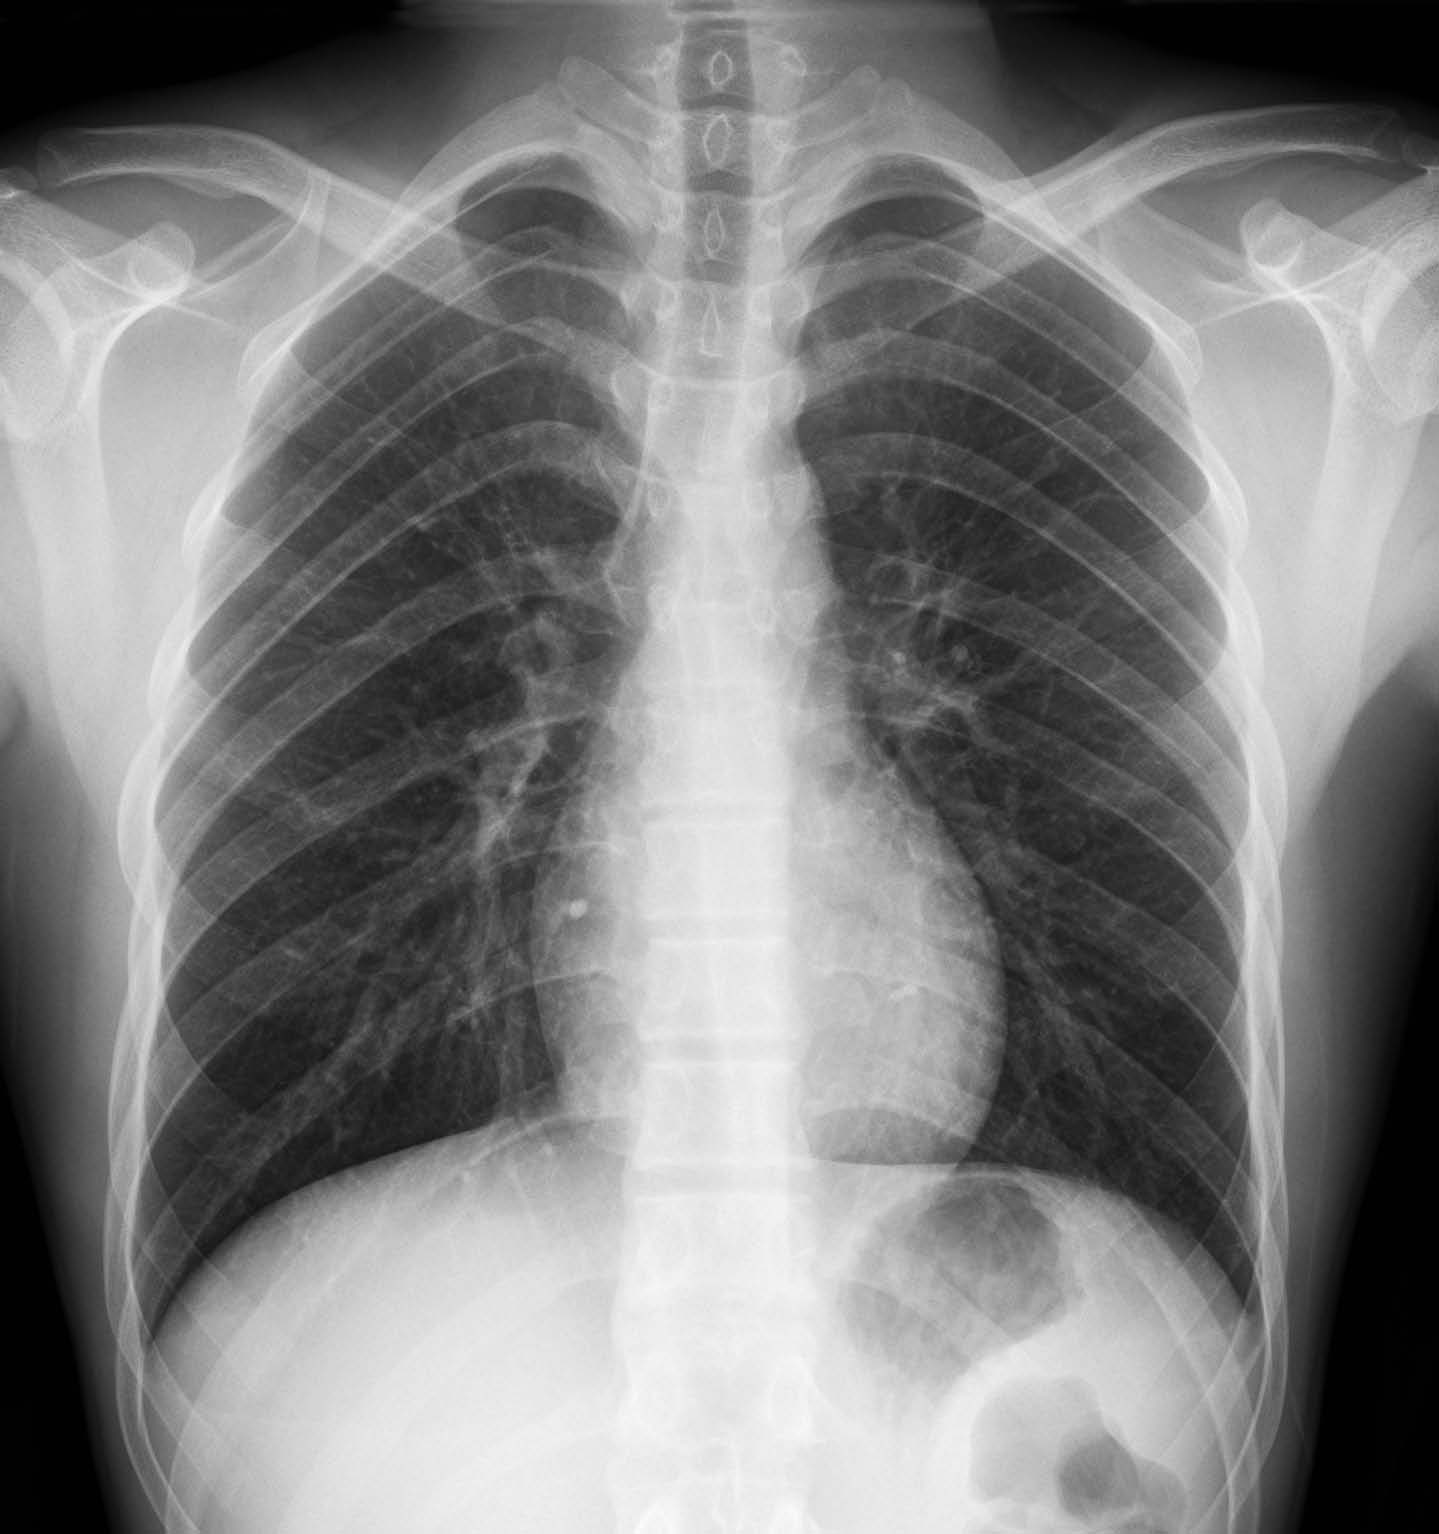
\includegraphics{./images/Image00129.jpg}
 \captionsetup{justification=centering}
 \caption{正常后前位X线胸片}
 \label{fig3-1-1}
  \end{figure} 

\begin{figure}[!htbp]
 \centering
 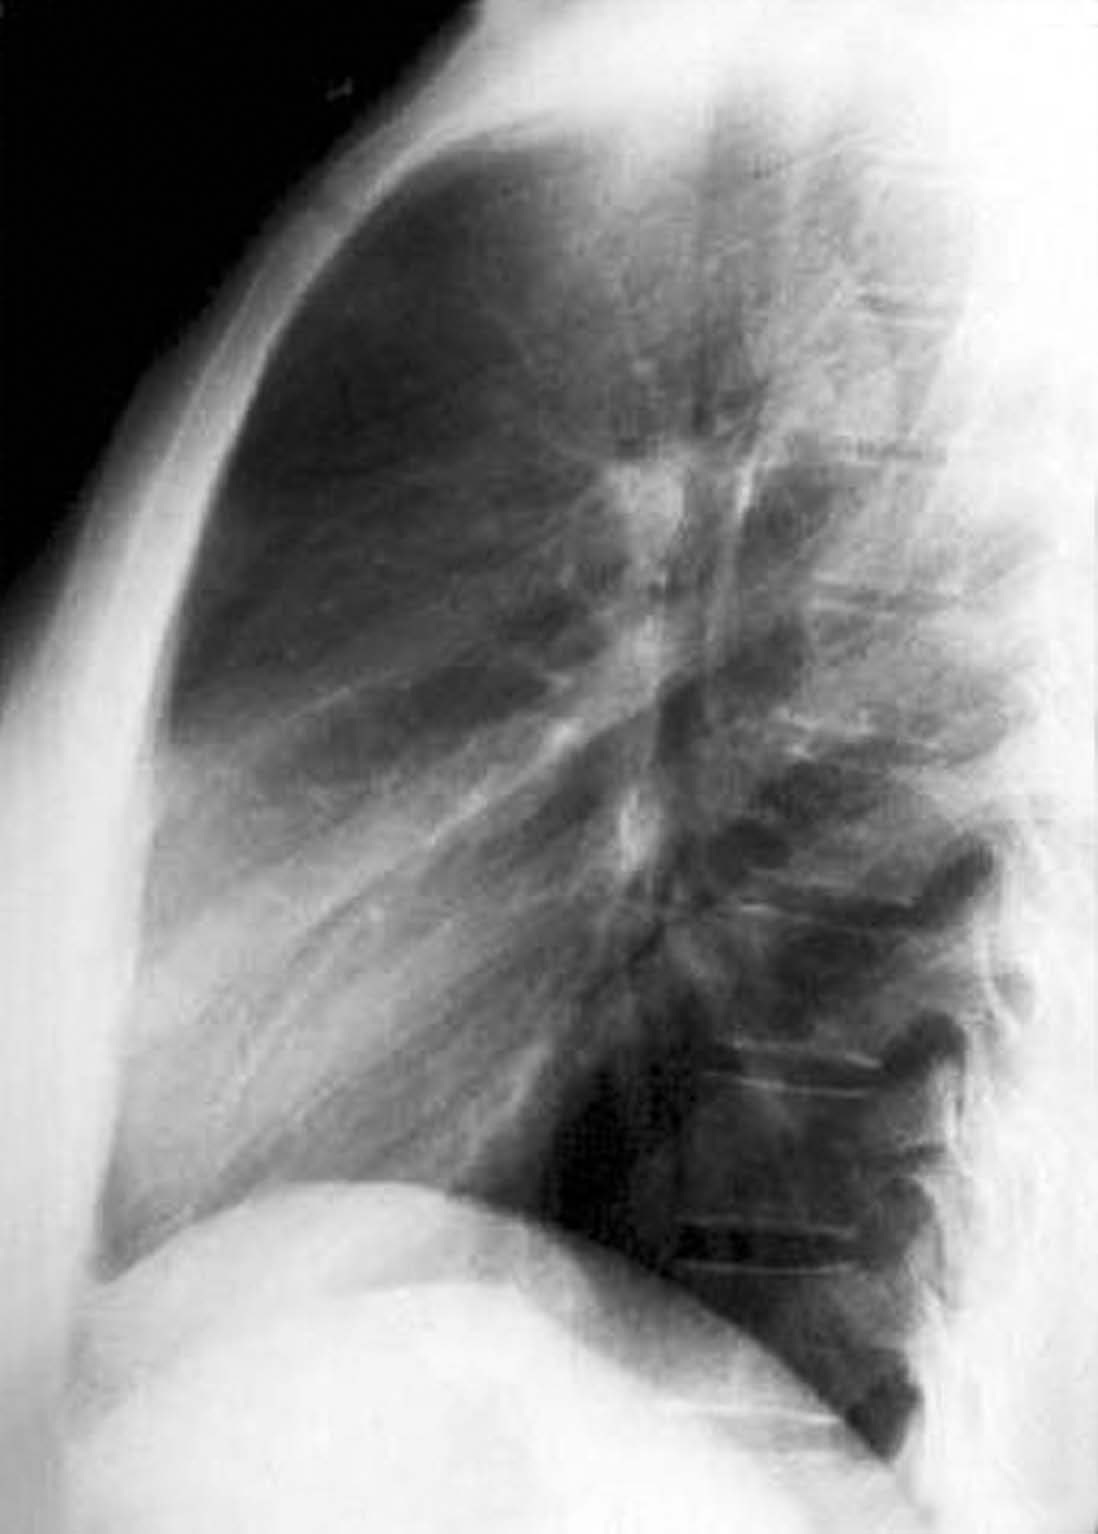
\includegraphics{./images/Image00130.jpg}
 \captionsetup{justification=centering}
 \caption{正常左侧位X线胸片}
 \label{fig3-1-2}
  \end{figure} 

一、胸廓

胸廓由骨骼及软组织构成,骨骼是决定胸廓形状的主要条件。胸廓软组织及骨骼在X线胸片上形成的正常组织影像,有时会误认为病变,应当知道这一点。

(一)软组织

1.胸锁乳突肌 胸锁乳突肌位于胸锁关节至乳突间,在两肺尖内侧形成外缘锐利、均匀致密、呈带状的影像。除可掩盖部分肺尖病变外,多无特殊意义。当头颈部摆位不正时,两侧胸锁乳突肌的阴影可不对称,勿误为肺尖病变。

2.锁骨上皮肤皱褶锁 骨上皮肤皱褶也称锁骨上伴随影,是锁骨上皮肤及皮下组织在锁骨上缘形成平行的3~5mm宽的条状软组织阴影,其内侧端与胸锁乳突肌呈圆角相交,外侧端则逐渐消失。该阴影较肺野密度高,而较锁骨密度低。当锁骨上淋巴结增大或有软组织肿块时,该影消失。反之,当该影显示不清者,应提示临床予以检查。

3.胸大肌 胸大肌的发育程度差别较大,男性体力劳动者往往很显著。胸大肌可在两侧中肺野的中外带形成扇形均匀致密影,其外下缘多锐利且可延伸至肺野以外,借此可与肺内炎症相区别。胸大肌影两侧可以对称,也可不甚对称,甚或可胸肌缺失(Poland综合征)。当两侧胸大肌发育不对称、一侧肿胀或缺失时,密度较高的一侧容易误认为肺内炎症,密度较低的一侧则易误认为肺气肿。乳腺癌根治术后,患侧密度明显减低,锁骨下区的胸大肌残端可形成一带状密度增高影,易将胸大肌残端误认为肺结核。也可将患侧误认为肺内炎症。

4.女性乳房及乳头 女性乳房随年龄变化其形状变化较大,基本上分三种类型。青春发育期者,乳房多小而坚实,于中肺野呈一片状密度稍高的阴影,边缘模糊不清;若两侧对称,识别无困难;若两侧不甚对称或身体稍有偏斜,则易将一侧显示清楚者误认为肺内炎症。中年妇女,特别是哺乳者,乳房脂肪增多呈丰满的半球状;于中、下肺野呈片状密度增高影,愈往上其密度愈浅淡,愈往下密度愈高,于膈肌附近常可见一弧形凸面向下的锐利边缘;丰满的乳房常可掩盖下肺野的病变,当掩盖肋膈角时,易误认为胸膜炎或掩盖胸膜炎症;识别困难时,透视检查有助于鉴别。老年妇女特别是瘦弱者,乳房小而低垂,乳房及胸大肌外缘与侧胸壁之间常示一纵行梭形的密度减低区,易误认为局限性气胸。当两侧乳房发育不对称或投照时体位欠正时,两侧阴影亦可不一致。一侧乳房单纯切除术后,患侧肺野密度减低,不要误认为肺内病变。

女性乳头可以成影或不成影,可在两下肺野相当于第5前肋间处形成小圆形致密影,年龄较大妇女多见,有时亦见于老年男性,勿误为肺内结节状病变。通常两侧对称,多呈直径约1cm大小密度增高的结节。但亦有仅见单侧者,可疑时可通过透视下转动患者即可明确,或采取乳头标记后照片加以确定。

\begin{figure}
  \centering
\subfloat[双侧正常女性乳头阴影(箭头)]{
\begin{minipage}[b]{0.7\textwidth}
\centering
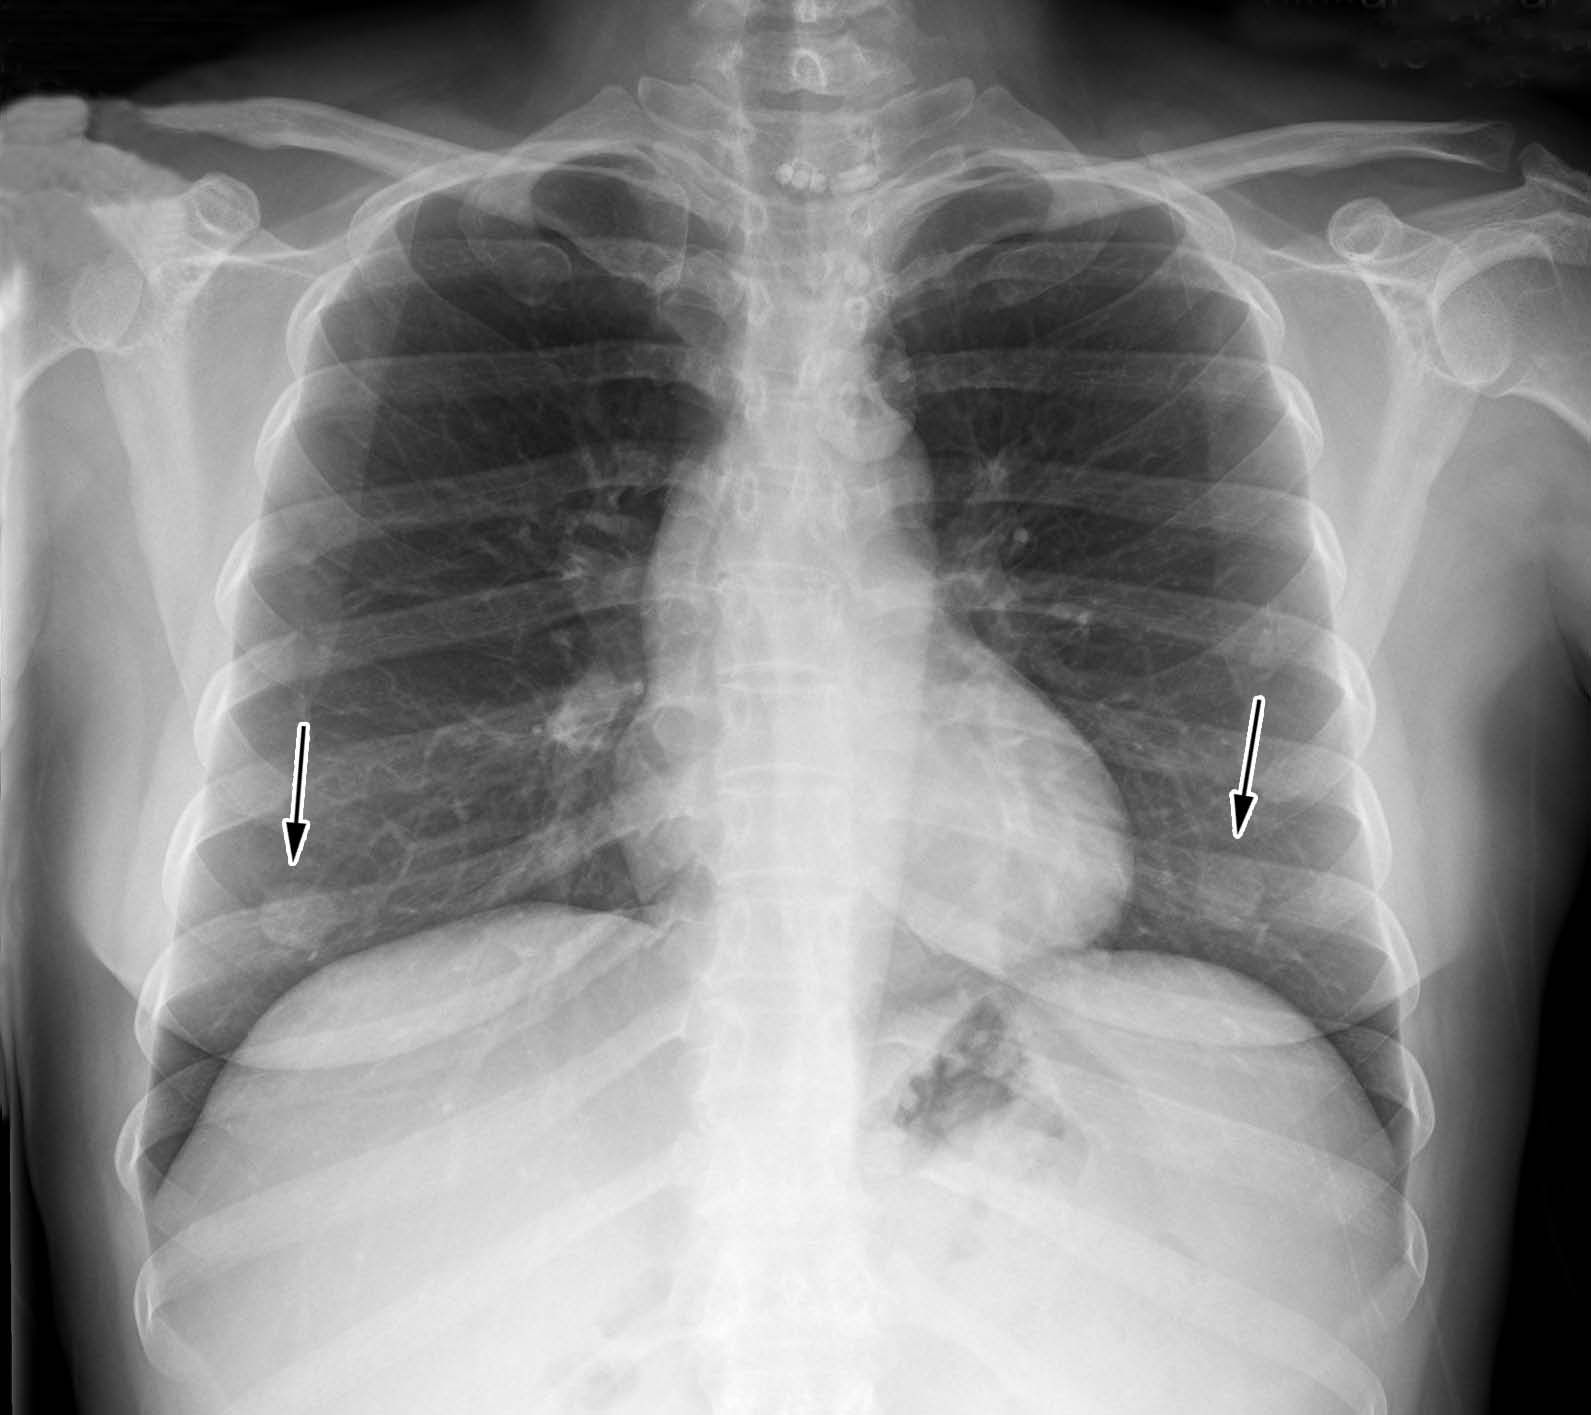
\includegraphics{./images/Image00131.jpg}
\end{minipage}}\\
\subfloat[双侧正常男性乳头阴影(箭头)]{
\begin{minipage}[b]{0.7\textwidth}
\centering
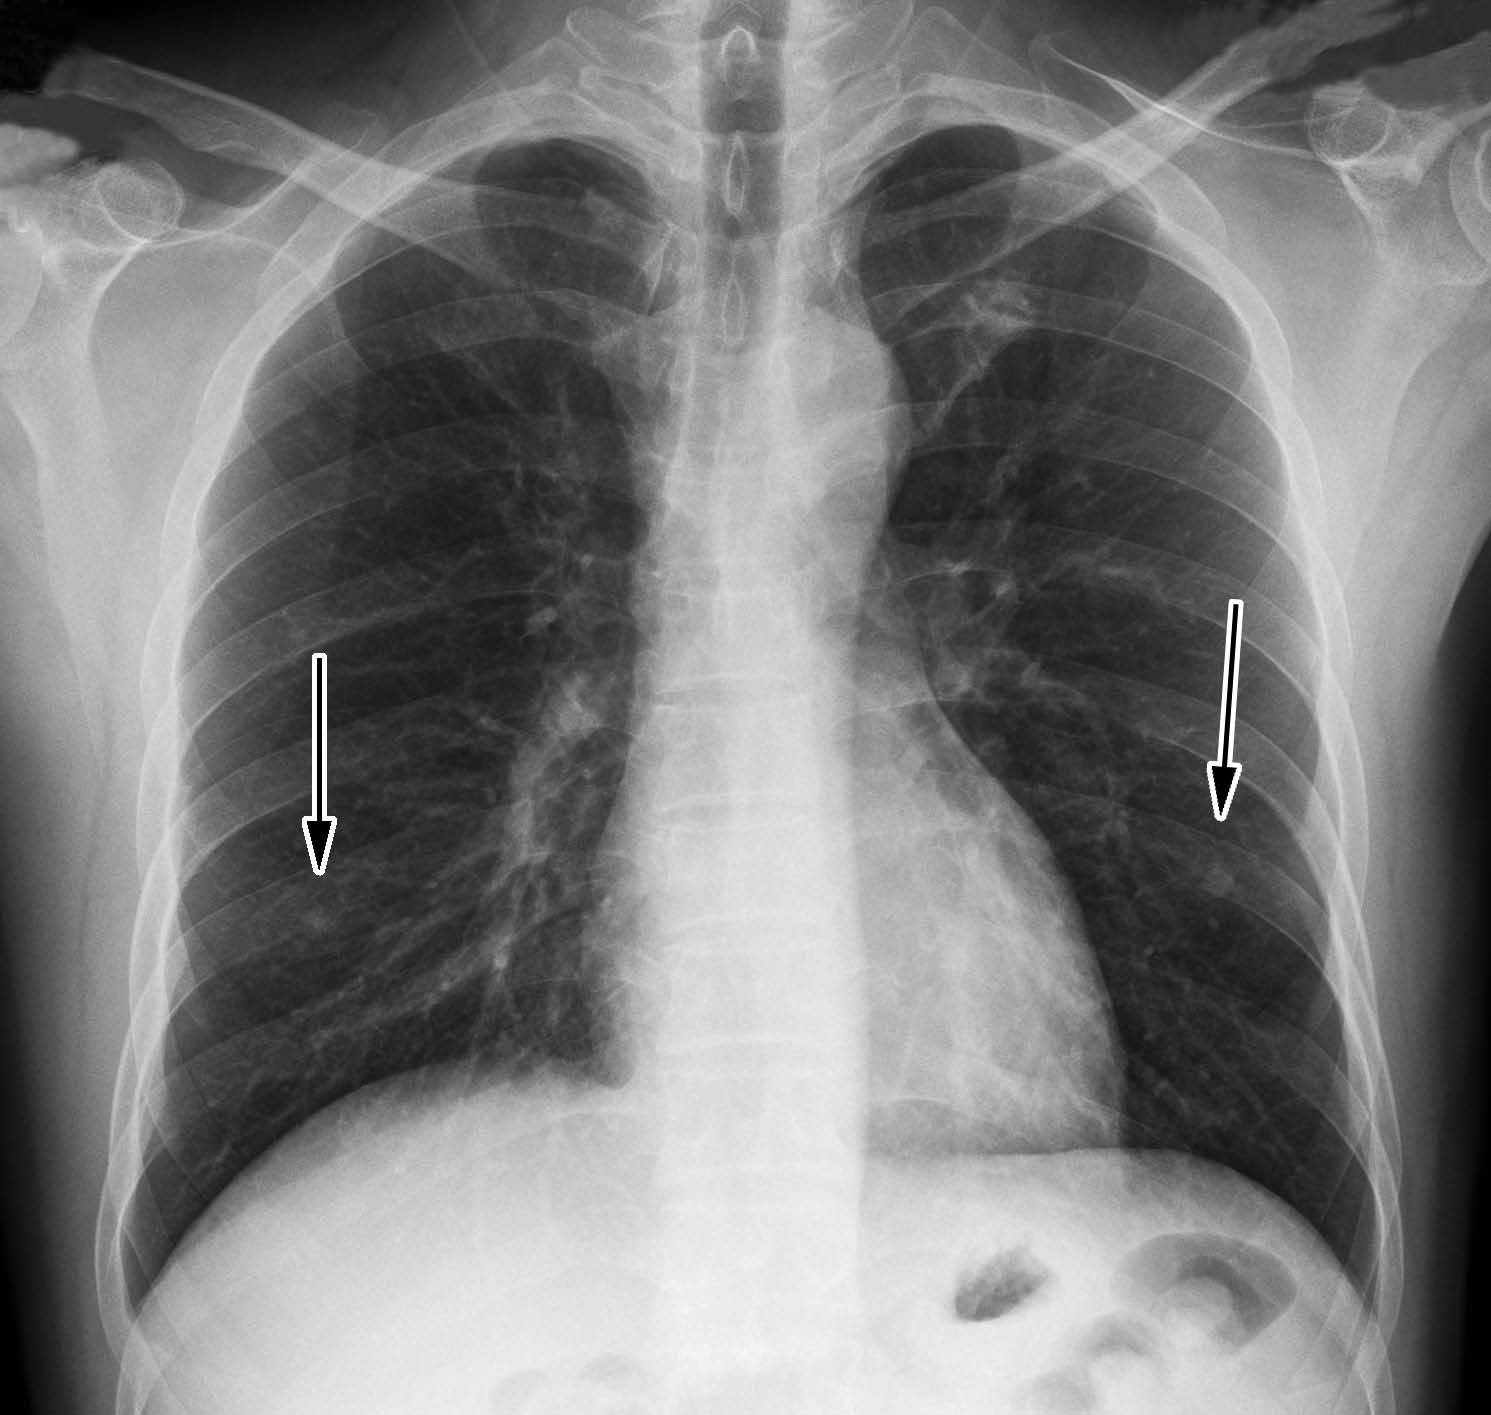
\includegraphics{./images/Image00132.jpg}
\end{minipage}}\\
\caption{}
\label{fig3-1-3}
\end{figure}

(二)骨骼

1.肋骨 肋骨起于胸椎两侧,左右对称,共12对。X线胸片上多能见到10对,第11、12肋骨不易显示。肋骨后段呈水平向外走行,前段自外上向内下倾斜走行形成肋弓。肋骨后端以肋骨小头及肋骨结节与胸椎及胸椎横突相连。肋骨前端借助软骨与胸骨相连。第11、12肋骨无肋软骨,也不与胸骨相连呈游离状称为浮肋。一般后10肋与前5肋骨在同一水平面上。相邻肋骨间的间隙称为肋间隙,两侧应等宽。由肋骨小头至腋中线的一段肋骨为肋骨后段,俗称后肋;由腋中线至肋骨前端的为肋骨前段,俗称前肋。两者区别如下:前肋宽而密度较低,后肋窄而密度较高;前肋自上外方向下内方走行,后肋自上内方向下外方走行,前肋只占据一侧胸腔的外、中部分,后肋则贯穿一侧胸腔;前肋间隙较宽,后肋间隙较窄;前肋的下缘多光滑整齐,后肋的下缘多呈花边状。

肋软骨多不成影,年龄较大时肋软骨呈条带状钙化,可在X线胸片上显示。第1肋软骨最先钙化,多在25~30岁出现,随着年龄增长,其他肋软骨自下而上逐根钙化,表现为条状或不规则斑片状致密影病变。若年龄较小而出现明显钙化时,应警惕有无钙、磷代谢性疾病存在。

肋骨的先天变异较常见,如颈肋、叉状肋、铲状肋、环状肋及肋骨联合等,不要误认为肺内病变。此外尚可见肋骨发育不良或肋骨缺如等。

2.肩胛骨 标准胸片上,肩胛骨的全部或绝大部分应不重叠于肺野内,有时肩胛骨的内缘可与肺野外带重叠,不要误认为胸膜增厚。若两肩向前旋转不足(或于仰卧位投照时),肩胛骨则可重叠于肺野的外上方,呈一梭形成片状的密度增高影,不要误认为胸膜的包裹性积液及肺内炎症。仔细观察,其边缘可延伸至肺野以外。侧位上,肩胛骨投影于气管后方,呈两条纵行的带状密度增高影,相互重叠密度更高。有时肩胛骨下角呈圆形密度增高影,勿误认为肺内球形病变。发育期的肩胛骨,其下角的二次骨化中心影不要误认为骨折。肩胛骨的先天性变异较少见。有时肩胛骨位置较高,称为翼状肩胛。

3.锁骨 锁骨为一横置的略呈S状的弯形骨,两侧对称。其内侧端与胸骨柄形成胸锁关节,外侧端与肩峰形成肩锁关节。X线上呈一横置的带状密度增高影,边缘光滑整齐。有时中心X线位置较低,特别在仰卧位投照时,锁骨可呈外侧端高内侧端低的曲线状,不要误认为骨折。有些患者于锁骨内侧端的下缘见一半圆形凹陷区,边缘可以规则或不规则,称为菱形窝,系菱形韧带(胸锁韧带)的附着所致,勿误认为骨质破坏。锁骨可有发育异常,如发育短小等。锁骨也可掩盖部分肺尖病变,但用前弓位检查有助于显示肺尖病变。

4.胸骨 胸骨位于胸前壁正中,是一块上宽下窄、前凸、后凹的扁骨,形似短剑,分为柄、体、剑突三部分。胸骨柄上缘中部微凹,叫颈静脉切迹,其两侧有锁骨切迹,与锁骨相关;柄侧缘接第1肋软骨;胸骨柄两侧外上角有时可突出于纵隔影之外,不要误认为纵隔病变。胸骨柄下缘与胸骨体连接处微向前突,称胸骨角(又叫Louis角),从体表可以触及;因其两侧恰与第2肋软骨相关,所以是确定肋骨序数的重要标志;胸骨角部位又相当于左、右主支气管分叉处,主动脉弓下缘水平、心房上缘、上下纵隔交界部,与背部第4、5胸椎相对应。胸骨体扁而长,两侧有第2~7肋软骨相连接的切迹。剑突形状多变,位居左右肋弓之间,有人终生保持软骨形式。

5.胸椎 正位上胸椎与纵隔影相重叠。照片条件适当时,透过纵隔影可以较清楚地显示胸椎及椎间隙。胸椎横突,特别是肺门部位,可突出于纵隔影之外,呈密度增高的结节状影,不要误认为淋巴结增大。横突与肋骨结节构成肋横突关节。投照角度合适时,肋横突关节可表现为一线状密度减低影。借其边缘有骨皮质的致密线影可与肋骨骨折相区别。

侧位上,特别是体胖的患者上部2~3个椎体及椎间隙多显示不清,其余胸椎椎体及其附件均可清晰显示。上部胸椎常轻微后凸,为正常之生理曲度。

胸椎侧弯为最常见的畸形。正位上示纵隔一侧性增宽,不要误认为纵隔肿瘤。尚可见胸椎发育异常、脊膜膨出及胸椎结核等,不要误认为纵隔肿瘤。

二、纵隔

纵隔是两侧闭合的胸膜腔之间的区域。前为胸骨,后为胸椎,上为胸腔入口,下为膈肌。纵隔由心脏、大血管、气管、支气管、食管、胸腺、淋巴组织、神经及脂肪等器官、组织构成。除气管及支气管可以辨认外,其他组织器官间无明显对比。正位上,呈一宽带状密度增高影,其边缘为心脏大血管的外缘。

为确定纵隔肿块的来源及其性质和叙述的方便,常将纵隔人为地分区。目前,常用的为九分区法:在侧位上将纵隔分为前、中、后及上、中、下九区。以气管前壁向下、沿升主动脉前缘及心脏前缘画一曲线,此线前方至胸骨的倒三角形之狭长区域为前纵隔。以食管后壁为界画线,该线后为后纵隔。两条线之间的区域为中纵隔。以第4胸椎下缘为点与胸骨角连接成线,其线上为上纵隔。以肺门下方,相当于第8胸椎下缘画一横线,该线上方为中纵隔,下方为下纵隔。该法较为实用,特别是前、中、后纵隔的分区对确定纵隔肿瘤的来源有帮助。

纵隔的长度和宽度受生理因素的影响。吸气状态、无力体形及立位时,纵隔影长而窄;呼气状态、矮胖体形及仰卧位时,其影短而宽。另外,小儿的胸腺常使纵隔向一侧或两侧增宽,勿误认为纵隔肿瘤。

\begin{figure}[!htbp]
 \centering
 
\includegraphics{./images/Image00133.jpg}
 \captionsetup{justification=centering}
 \caption{纵隔分区线图}
 \label{fig3-1-4}
  \end{figure} 

\begin{figure}[!htbp]
 \centering
 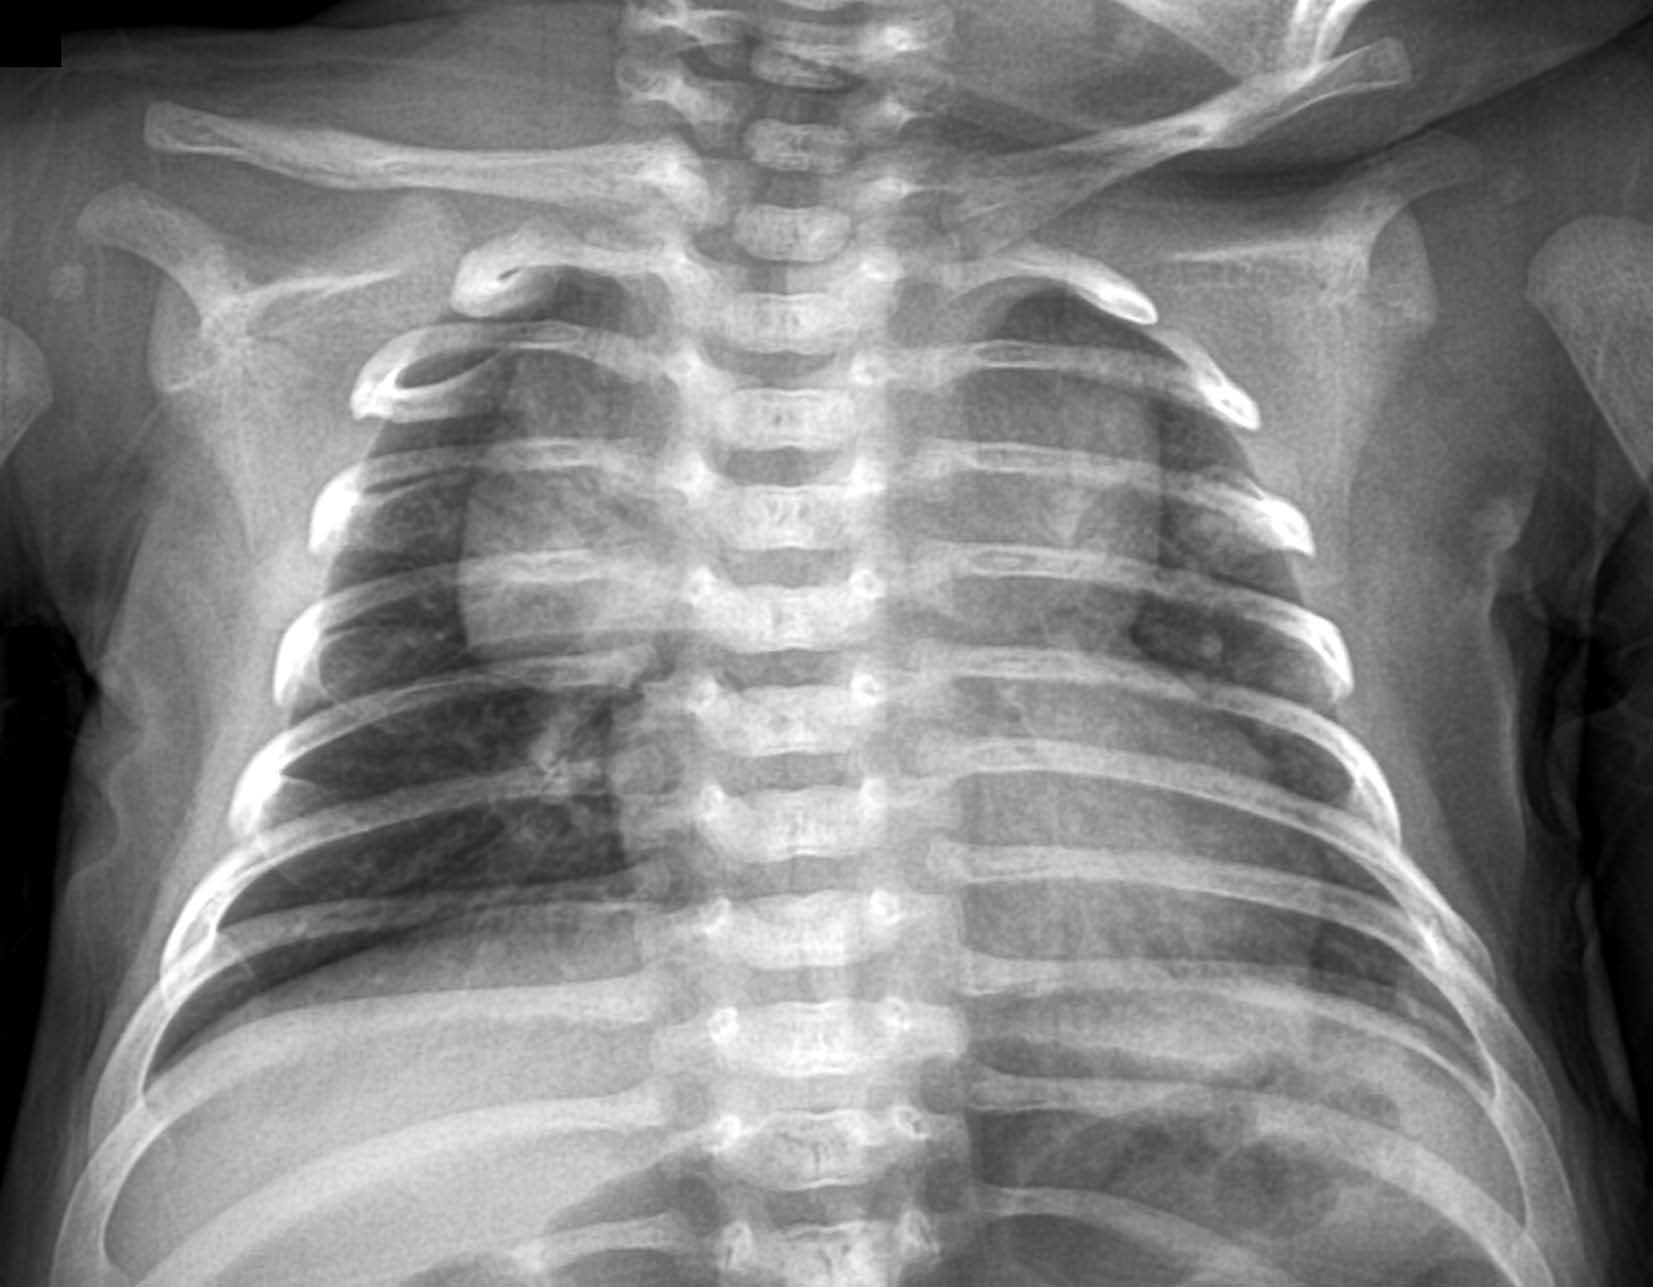
\includegraphics{./images/Image00134.jpg}
 \captionsetup{justification=centering}
 \caption{儿童胸腺呈帆影状}
 \label{fig3-1-5}
  \end{figure} 

三、膈

膈肌为介于胸、腹腔之间的薄的肌腱膜。分左、右两叶,呈凸面向上的圆顶状。中央部分与心脏相连接。膈肌与侧胸壁形成的锐角称肋膈角。膈肌与心脏边缘形成的锐角称心膈角。但在左侧,特别是体胖者,其密度常较高、角度可以变钝,为心包脂肪垫所致,不要误认为病变。侧位上,膈肌呈前部高、后部低的凸面向上的曲线状,与前、后胸壁形成肋膈角,立位时,后肋膈角位置最低,是少量胸腔积液的汇集区域。前肋膈角由于心包脂肪垫的影响可不甚锐利及清晰,不要误认为胸膜病变。

两侧膈肌的位置常不等高,右侧较左侧高1~2cm,右侧膈肌常位于第6前肋与第10后肋水平。吸气时,膈肌下降;呼气时,膈肌上升。两侧膈肌动度相等或近似,两侧的活动度差不超过1cm且运动方向一致。一般认为,平静呼吸时膈肌活动度1~3cm;深呼吸时3~6cm。膈肌受生理因素影响,位置可有变化。吸气状态、无力体形及立位时,膈肌位置低;而呼气状态、体胖、卧位或妊娠后期,则膈肌位置高。

有时,膈肌的内1/3呈向上的局限性隆凸,边缘光滑整齐,为局限性膈膨出。右侧较左侧多见,年老者多见,无病理意义,属正常变异;应与肝脏的局限性隆凸相区别,区别困难时,行CT等影像检查有帮助。有时深呼气时,膈肌为3~4个浅弧形向上隆凸的影像,呈波浪状,称为波浪膈,无病理意义,不要误认为胸膜粘连。

四、胸膜

胸膜菲薄,分包裹肺与叶的脏层胸膜和与胸壁、纵隔及横膈相贴的壁层胸膜,两层胸膜之间为潜在的胸膜腔,内有少量液体,起滑润作用。正常时胸膜在X线上不显影,但在胸膜返折处且X线与胸膜走行方向平行时,胸膜可显示为线状致密影。肺叶之间的胸膜称叶间胸膜,其间的裂隙称为叶间裂,有水平裂和斜裂之分;水平裂为右肺上叶与中叶之间的叶间裂;斜裂为右上、中叶与下叶间的右侧叶间裂及左上叶与下叶间的左侧叶间裂。常规胸部正位片多可见水平裂胸膜,表现为从腋部第6肋骨水平向内止于肺门外1cm处的水平线状致密影。侧位片上,斜裂胸膜表现为自后上(第4、5胸椎水平)斜向前下方的线状致密阴影,在前肋膈角后2~3cm处与膈肌相连;水平裂起自斜裂中点,向前水平走行达前胸壁。

肺叶间裂的变异常见的有奇叶、奇裂,系肺的发育过程中,奇静脉被包入发育中的右肺叶内,由奇静脉两侧的四层胸膜折叠形成,表现为自右肺尖部向奇静脉方向走行的弧形线状致密影(即奇裂),以小圆点状的奇静脉为终止点,其内侧肺组织即奇叶。

五、气管、支气管

气管起自环状软骨下缘,经颈部进入胸腔。在胸椎5~6平面分为左、右主支气管。左、右主支气管(一级)分别进入左、右肺,其分支角称为隆突角为60°~80°。吸气时该角度变小,呼气时则变大,相差10°~15°。右侧主支气管近似于气管的延续,与气管延长线呈20°~30°角;宽度较宽而长度较短,约2.5cm长;右侧主支气管分为三支,分别进入上、中、下三个肺叶,称为肺叶支气管(二级);右侧主支气管发出上叶支气管后,直至中叶开口的一段支气管为中间支气管。左侧主支气管与气管的延长线呈40°~50°角;较细,但较长,约5cm长;左侧主支气管分为二支,分别进入上、下肺叶。肺叶支气管再分支为肺段支气管(三级),以后逐次分支为肺亚段支气管、肺小叶支气管、末梢细支气管、呼吸细支气管等。除呼吸细支气管具有呼吸功能外,其他支气管均为气体的通道。

\begin{figure}[!htbp]
 \centering
 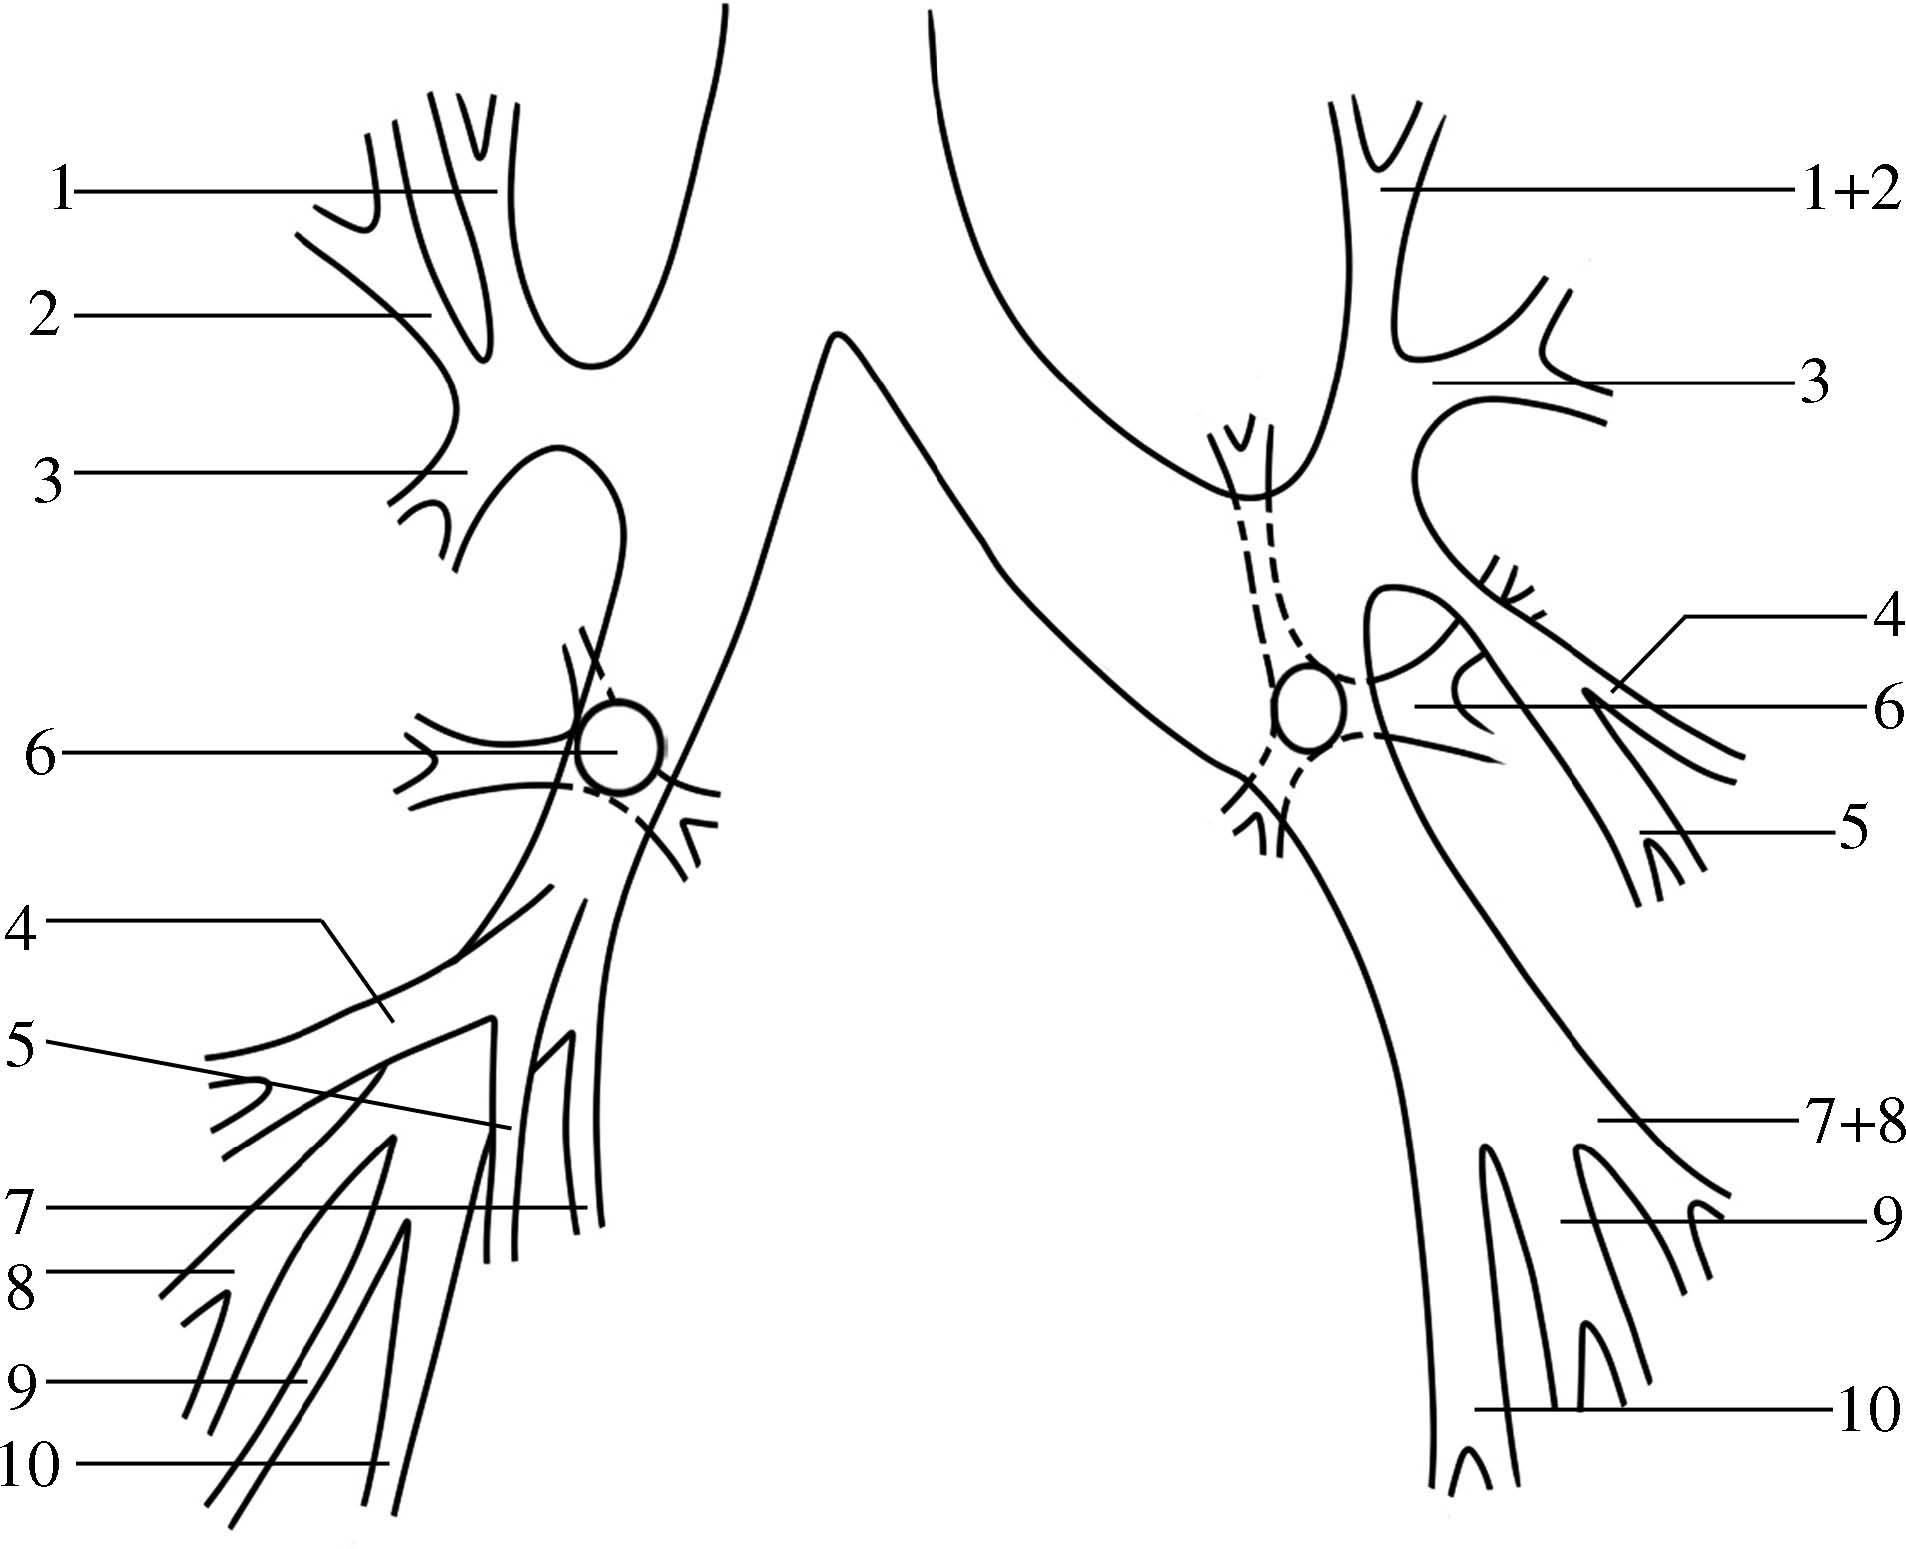
\includegraphics{./images/Image00135.jpg}
 \captionsetup{justification=centering}
 \caption{支气管分支线图\\{\small 右侧:1.尖支2.后支3.前支4.外支5.内支6.背支7.内基底支8.前基底支9.外基底支10.后基底支\\ 左侧:1+2.尖后支3.前支4.上支5.下支6.背支7+8.前内基底支9.外基底支10.后基底支}}
 \label{fig3-1-6}
  \end{figure} 


以往,常规X线上最常显示的是气管,目前的数字化摄影也能显示支气管,但也只限于肺叶及部分肺段支气管。其先天性变异主要为分支异常,胸片难以显示,需CT三维成像或支气管造影证实。

六、肺

(一)肺野

充满气体的两肺在胸片上表现为均匀一致较为透明的区域称肺野。两侧肺野透明度基本相同,其透明度与肺内所含气体量成正比。为叙述方便,通常将第1肋圈内的部分称为肺尖;接近膈肌的部分称为肺底;以第2与第4前肋下缘分别画一条横线,将肺野分成三部分为上、中、下三个肺野;以胸廓形状将一侧肺野纵行分成三等份,由内向外为内、中、外三带。

\begin{figure}[!htbp]
 \centering
 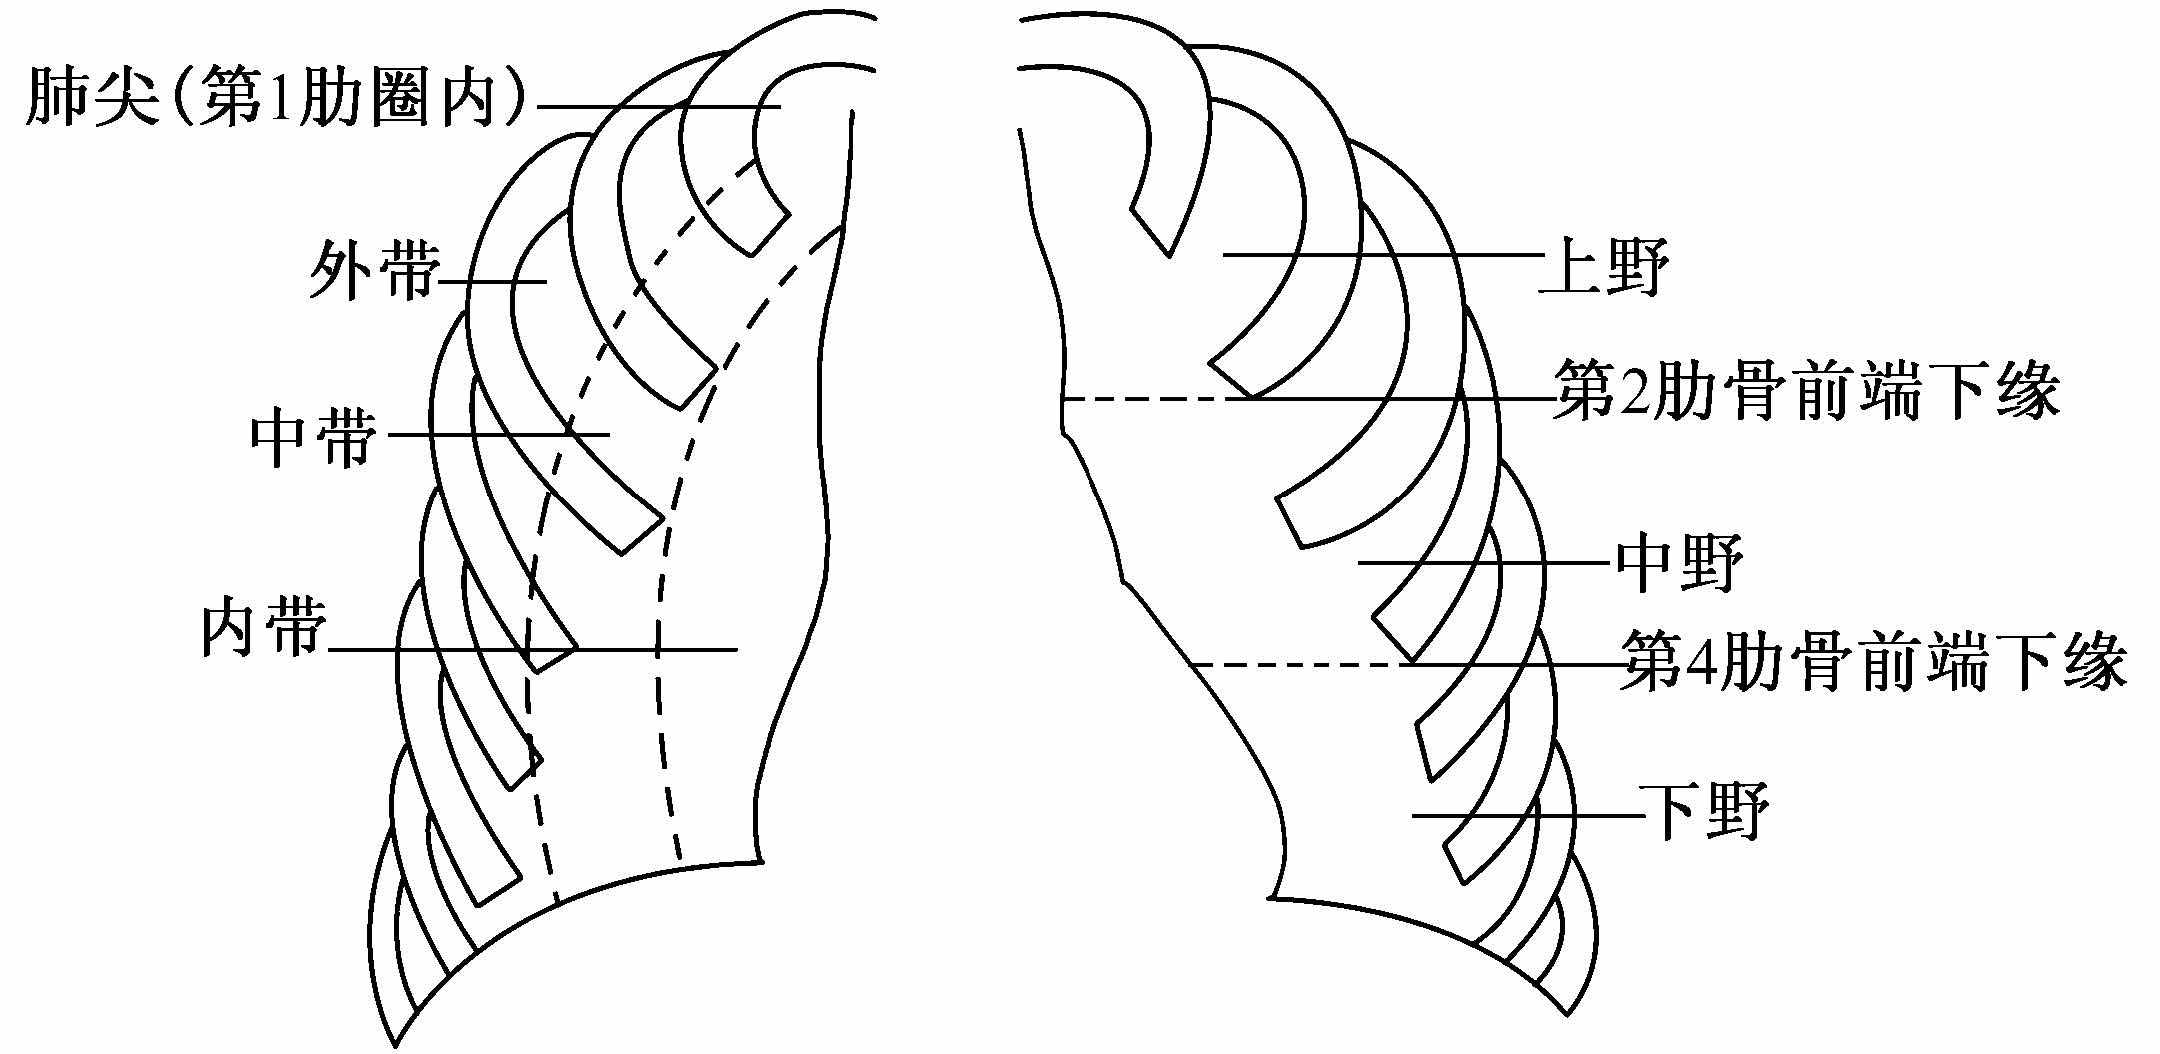
\includegraphics{./images/Image00136.jpg}
 \captionsetup{justification=centering}
 \caption{正常肺野划分线图}
 \label{fig3-1-7}
  \end{figure} 

(二)肺门

胸片上肺门影是肺动脉、静脉、支气管及淋巴组织的复合影,其中肺动脉和肺静脉的大分支为主要成分;后前位胸片上,肺门位于两肺野内带第2至第4前肋间处,左肺门较右侧高1~2cm,两侧肺门可分上、下两部。上、下部相交形成一钝夹角,称肺门角,而相交点称肺门点,右侧显示较清楚,呈横写的V形。右下肺动脉内侧有含气的中间支气管衬托而轮廓清晰,正常成人其横径不超过15mm。左下肺动脉由于心脏影的遮盖不能见其全貌。侧位胸片上两侧肺门大部重叠,右肺门略偏前,肺门表现似一尾巴拖长的“逗号”,其前缘为上肺静脉干,后上缘为左肺动脉弓,拖长的逗号尾巴由两下肺动脉干构成。

两侧肺门区常可见到2~3mm大小、周围密度高、中间透亮的环状影,系支气管的轴位投影。与其伴行的为大小近似密度高的点状影、边缘清楚,为血管的轴位投影。

由于肺门大小的正常差异较大,除右下肺动脉有一测量值外,余者几无正常标准,因此判断肺门是否增大或缩小,需慎重,并注意随访复查,观其变化。此外,尚需注意观察右肺门角的情况,若右肺门角呈反弧状,常为肿块或肿大的淋巴结所致。肺门的密度及其锐利程度亦应重视。

(三)肺纹理

在充满气体的肺野,可见自肺门向外呈放射分布的树枝状影,称为肺纹理。肺纹理由肺动脉、肺静脉组成,其中主要是肺动脉分支,支气管、淋巴管及少量间质组织也参与肺纹理的形成。在正位胸片上,肺纹理自肺门向肺野中、外带延伸,逐渐变细,至肺野外围几乎不能辨认。下肺野肺纹理比上肺野多而粗,右下肺野肺纹理比左下肺野多而粗。应该指出肺纹理正常粗细和多少并无明确标准,但变化明显时则不难确定。肺纹理是否显得松散,特别是聚拢,有时更有临床意义。

(四)肺叶、肺段和肺小叶

1.肺叶 是被脏层胸膜分隔的解剖单位,由叶间胸膜分隔而成,右肺分为上、中、下三个肺叶,左肺分为上、下两个肺叶。肺叶与肺野的概念不同,肺叶前后重叠。每个肺叶由2~5个肺段组成,每个肺段有单独的段支气管。胸片上,借显影的叶间胸膜可分辨肺叶,多不能完整地显示肺叶的界限,但结合正侧位胸片常可推断各肺叶的大致位置,从而确定病变的部位。右肺上叶位于右肺前上部,上缘达肺尖,下缘以横裂与中叶分隔,后缘以斜裂与下叶为界;右肺中叶位于右肺前下部,上缘以横裂与上叶为界,下缘以斜裂与下叶分隔,自横裂最外端向内、向下斜行至右膈内侧部,内界直达右心缘,呈三角形;右肺下叶位于右肺后下部,以斜裂与上叶及中叶分界。左肺上叶相当于右肺上叶和中叶所占据的范围;左肺下叶相当于右肺下叶所占据的范围。正位胸片上,上叶下部与下叶上部重叠,中叶与下叶下部重叠。侧位胸片上,上叶位于前上部,中叶位于前下部,下叶位于后下部,彼此不重叠。

副叶是由副裂深入肺叶内形成,属于肺分叶的先天变异。奇叶为常见的变异,因奇静脉位置异常,奇静脉与周围的胸膜反折形成奇副裂,分隔右肺上叶内侧部分成为奇叶。奇副裂呈细线状影,自右肺尖部向内、下走行至肺门上方,终端呈一倒置的逗点状,是奇静脉断面的垂直投影。

2.肺段 肺段组成肺叶,常呈圆锥形,尖端指向肺门,底部朝向肺的外围,肺段间没有明确边界。各肺段的名称与其相应的支气管一致。正常时,X线片不能显示肺段的界限,只有在病理情况下,某个肺段受累时才能看到肺段的轮廓。右肺上叶由尖段、后段及前段所组成;中叶由内侧段及外侧段组成;下叶由背段、内基底段、后基底段、外基底段及前基底段组成。左肺上叶分为上部和舌叶两部分,上部由前段和尖后段所组成;舌叶由上舌段和下舌段组成;下叶由背段、后基底段、外基底段及前内基底段组成。

3.肺小叶 每一肺段由许多肺小叶组成,肺小叶既是解剖单位又是功能单位,直径为1~3cm,小叶之间有小叶间隔。每支小叶支气管分出3~5支末梢细支气管,每支末梢细支气管所支配的范围称为腺泡,为肺部病理改变的基本单位,其直径约6mm。末梢细支气管继续分出呼吸细支气管,以后再分肺泡管、肺泡囊,最后为肺泡。肺泡壁上有小孔,称为肺泡孔,空气可经肺泡孔相互沟通。呼吸细支气管、肺泡管、肺泡囊、肺泡为肺的气体交换部分。正常胸片上不能显示其轮廓,单个肺小叶实变可表现为直径1~3cm的片状影。当腺泡范围内发生实变时,胸片上可表现为类圆形结节状致密影,称腺泡结节样病变。

4.肺实质与肺间质 肺组织由肺实质和肺间质组成。肺实质包括肺泡、肺泡囊、肺泡管及1~3级呼吸性细支气管,主要功能为储存气体和气体交换。肺间质包括支气管、血管、淋巴管及其周围的疏松结缔组织等,它无气体交换功能,只起支持作用。X线上不能将两者截然分开。即或有炎症时,也是以其中一种炎症为主,两者亦难截然分开。

七、胸部X线诊断的原则

(一)系统周密的观察

要想做出正确的诊断,必须从系统周密的观察开始。观察的要求和内容包括以下几方面。

1.X线片的技术条件 阅读分析X线片时,首先应注意照片的质量,是否符合诊断的要求。一张良好的照片,必须达到:位置正确,黑白对比鲜明,细微结构清晰可见,照片清洁不带污迹及其他伪影,标记(左、右及片号等)鲜明无误。

2.按一定程序观察X线片 为了不至于遗漏重要X线征象,应按一定顺序,全面而系统地进行观察。如以胸片为例,应按胸廓、肺、纵隔、横膈及胸膜等逐步观察。在分析肺部的X线表现时,可从肺尖到肺底,从肺门到肺周依次进行观察。否则很易被引人注目的部分所吸引,忽略观察其他部分,而往往这些部分正是更重要而必须阅读的部分。

3.对病变观察的要点

(1)病变的部位和分布:某些病变好发于人体的一定部位,它的分布可表现出一定规律。后纵隔肿瘤多为神经源性肿瘤,而中纵隔的肿瘤则多为淋巴类肿瘤等。

(2)病变的数目:病变的数目常与其性质有关。肺内转移瘤常为多发,而原发性周围性肺癌多为单发。

(3)病变的形状:肺内斑片状阴影多为炎症;而球形阴影多为肿瘤,有时亦可为结核球或炎性假瘤。

(4)病变的大小:在肺内弥漫性病变中,急性粟粒性结核,其斑点状阴影直径为1~2mm,矽肺结节一般为2~4mm;而转移瘤的斑点,因转移时间不一,往往大小不一。

(5)病变的边缘:肺内良性肿瘤边缘光滑锐利,恶性肿瘤边缘呈分叶状,并见细小毛刺;肺内炎症往往边缘模糊不清。

(6)病变的密度:病变的密度可以较周围组织增高或减低。浸润型肺结核初期病灶的密度较为浅淡,当硬结钙化时密度增高。又如2cm以下周围性肺癌,病灶往往密度不均匀,可见颗粒征、空泡征,而3cm以上病灶通常密度增加且均匀一致。

(7)器官本身的功能变化:左心功能不全时可出现肺瘀血,甚至肺水肿;慢性支气管炎伴肺气肿患者,透视下呼吸改变时,横膈移动甚小,肺野透亮度改变甚微,反映患者换气功能下降。

(8)病变周围的组织结构:观察病变时,其周围情况也应有所了解,才能使诊断正确全面。如中央型肺癌,早期可致肺外围出现阻塞性肺气肿,而后可引起阻塞性炎症,甚至出现肺不张,局部肋间隙变窄,同侧膈肌升高,更有甚者出现局部肋骨破坏。又如结核球,其周围往往可见斑点条索状影,即所谓卫星灶。

4.掌握临床情况对患者的临床情况,除病历中或检查申请单上记载外,根据诊断需要,有时可亲自做进一步询问和必要的体格检查。也可与临床医师共同研究,以便掌握更可靠和全面的临床资料,这对完成正确的X线诊断是非常重要的。

(二)客观的逻辑分析判断

当我们通过对X线影像的观察取得了丰富的材料后,产生了许多印象,必须经过科学地分析和研究,才能得出准确的结论。在进行综合分析时,如何使X线表现紧密与临床资料结合起来,这是非常重要的。以下问题值得注意。

1.性别 有些疾病的发生,与性别有一定关系,如风湿性心脏病多发生于30岁以上女性。

2.年龄 根据受检者的年龄对疾病进行分析。如儿童肺内肿块,多为良性:而老年则多为恶性。冠状动脉粥样硬化性心脏病多于40岁以上发病,而原发性心肌病发病年龄偏轻。如原发性肺结核多见于儿童及青少年;支气管肺炎多见于儿童及体弱年老者。

3.体形 人的体形对心脏方面影响较明显。如瘦长者心脏多呈垂位心,而矮胖者心影多呈横位。因此,对瘦长人来说,如出现横位心时,往往提示心脏增大。

4.职业史和接触史 受检者的职业与接触史为诊断职业病和寄生虫病的重要依据,如在诊断尘肺或放射损伤等,则均应具有特殊的职业史和接触史;在诊断肺部血吸虫病时,必须询问是否有疫水接触史。

5.生活史 在诊断地方病或区域性疾病时,应详细了解受检者的生长和居住过的地区,这对确定某些疾病的性质是有决定作用的。如包虫病多发生于西北牧区,而华东地区则有血吸虫病。

6.过去史 病史对决定病变的急性与慢性有很大帮助。如位于肺底部斑片状模糊阴影,如系发病突然且伴有发热、咳嗽、胸痛者,可诊断为急性肺炎;而对病程较久,又有长期咳嗽、咳痰与咯血者,则应考虑为支气管扩张并感染的可能;如在一个局部反复出现炎症,年龄偏大,应想到阻塞性肺炎的可能。

7.体征 心脏病的早期或心脏的X线征象改变不典型时,心脏听诊更为必要,对肺瘀血、心影呈梨形的患者,胸骨左缘第2至第3肋间闻及较柔和的收缩期杂音,多为房间隔缺损;胸骨左缘第3至第4肋间闻及粗糙响亮的收缩期杂音,可叩及震颤,多为室间隔缺损;胸骨左缘第2肋间闻及滚筒样连续性杂音,则多为动脉导管未闭;听到心包摩擦音或心音遥远者,应想到心包炎。

8.重要的检查结果 临床检验结果,对分析病变性质和确定X线诊断也是非常重要的。如在痰中发现结核杆菌时,上肺野出现斑片状阴影,应首先考虑为肺结核。

9.治疗经过 对某些X线影像一时难以确定其性质时,可通过诊断性治疗,观察病灶的变化,最终给予判断。如在肺部发现片状阴影,而临床症状轻微,经过抗感染治疗后阴影消失,则可诊断为肺炎而不是结核。

应该指出,X线诊断是有价值的,但也有一定的限制。传统X线检查只能分辨四种密度,如只能诊断胸腔积液,而无法区别是脓胸、血胸或胸水;有些疾病临床表现已经出现,而X线可暂时表现为阴性,如大叶性肺炎等。

(三)以疾病的病理变化过程来推演出胸部病变的影像变化

肺部病变的影像是肺内病变病理变化过程中的某个时间点在X线影像上的反映。某一疾病在病理变化过程中不同的时间点上,其所反映的X线影像是不同的,如大叶性肺炎,在不同的病理期,其X线影像各不相同,即所谓同病异影;不同的疾病在病理变化过程中,某个时间点的X线影像可有相同的交叉点,如亚急性肺结核与尘肺,其肺内均有增殖性肺结节,在X线影像上表现相仿,难以区分,即所谓异病同影。所以,作为影像诊断医师,应熟知各疾病的病理变化过程,病变的X线影像及不同的临床表现是疾病病理变化过程中不同阶段的反映。疾病的病理变化过程是一个动态的过程,不同的病理时间点其影像表现不同,在实际工作中,切忌以专业教科书中所示疾病的典型影像表现来用静止的观点解释X线征象,要用动态的观点来看待问题。疾病的X线征象均有其病理变化基础,要用疾病的病理变化来解释X线影像,脱离疾病的病理变化知识,是学不好X线影像诊断的。

总之,X线诊断结果基本上有三种情况:①肯定性诊断,即确诊。②否定性诊断,即经过X线检查,排除了某些疾病,此种判断应慎重,因有时X线表现比临床与体征有滞后现象,必需跟踪观察。③可能性诊断,即经过X线检查,发现了某些X线征象,但一时难以明确性质,可列出几种可能性,当然可能性最大者应放在首位。

\section{气管和支气管疾病}

\subsection{先天性支气管闭锁}

\begin{figure}[!htbp]
 \centering
 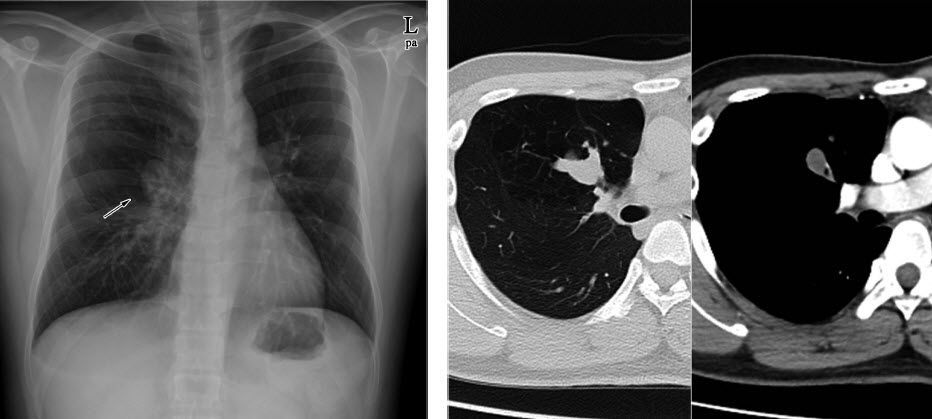
\includegraphics{./images/Image00137.jpg}
 \captionsetup{justification=centering}
 \caption{胸部X线正位和增强CT}
 \label{fig3-2-1}
  \end{figure} 

\textbf{【病史摘要】}
 男性,28岁。10余年前X线胸片发现右肺结节。平常自觉无明显不适,偶有轻微活动后气喘。

\textbf{【X线表现】}
 双侧胸廓对称。气管居中。右肺门处见类圆形结节影(箭头),无明显分叶,境界清晰,密度均匀,瘤内未见明显钙化,邻近肺野见局部透亮区,右下肺纹理增粗紊乱。左肺野未见明显异常。心脏大小属正常。双侧肋膈角锐利。胸部增强CT可见无强化的右肺上叶前段分支状粘液栓塞及所属肺组织气体潴留形成的气肿区。

\textbf{【X线诊断】}  右肺上叶支气管粘液栓可能,伴周围气肿。

\textbf{【评  述】}  支气管闭锁(Bronchial
atresia)是一种罕见的因近段支气管或亚段支气管局部闭塞引起的先天性发育异常,由Falor和Kyriakies于1949年首先报道,属于先天性支气管畸形的范畴,常与这一类的其他畸形,如叶内型肺隔离症、先天性支气管囊肿、先天性肺气道畸形、心包缺损、肺静脉异位引流等并存。本病可发生于任何年龄,但相当一部分患者临床上并无症状,所以该病的诊断通常在20~40岁时做出,多以偶然发现的孤立性肺结节而就诊。部分患者临床上有咳嗽、呼吸困难、反复呼吸道感染、喘息乃至咯血等症状,肺功能显示阻塞性通气障碍,往往年龄越小,症状越重。本病特征性的影像学表现是某一肺段或肺叶支气管内粘液栓塞,其近端的支气管腔闭锁、远端的肺组织气肿,唯有此三个征象同时显示时方可诊断本病。X线平片上最常见的表现是肺门周围结节状或管状密度增高影,闭锁远端的肺组织在新生儿期因支气管闭塞,肺液清除延迟而形成肺段形态的密度增高影,肺液清除后由于侧枝通气的存在而气体潴留,透亮度增加,肺纹理减少,可伴或不伴非特异性的炎性浸润。以左肺上叶尖后段最好发,其次是右肺上叶和下叶,右肺中叶最少见。通常,病变只累及单一的肺段,但多肺段受累的病例也时有报道。胸部CT表现与X线平片类似,能更好地显示支气管闭锁的各种征象,增强CT能通过有无强化区分闭锁远端支气管的粘液栓塞和血管畸形。动态CT呼气相扫描能更清晰的显示闭锁支气管远端肺组织的气体潴留情况。

本病常需与支气管肿瘤、炎症性病变、支气管异物、良性支气管狭窄等阻塞支气管而形成粘液栓的病变相鉴别。在成人,引起支气管粘液栓塞最常见的疾病是支气管肺癌,以大气道多见,也可见于支气管腺瘤和结肠腺癌支气管内转移等。肿瘤性病变除粘液栓塞外还可以看到肿块影,可伴远端肺组织的不张。炎症性疾病中以过敏性支气管肺曲菌病最多见,但其常累及多个肺叶,粘液栓塞为一过性改变,也不伴远端肺组织的气肿,且多见于段及段以远的支气管。良性支气管狭窄常仅表现为段或亚段支气管粘液栓形成,而无周围肺实质内过度气体潴留形成的气肿区。动静脉畸形、肺静脉异位引流等血管畸形在X线平片上也可和粘液栓塞的影像混淆,增强CT检查能有效的将之区分开来。

\subsection{先天性支气管囊肿}

\begin{figure}[!htbp]
 \centering
 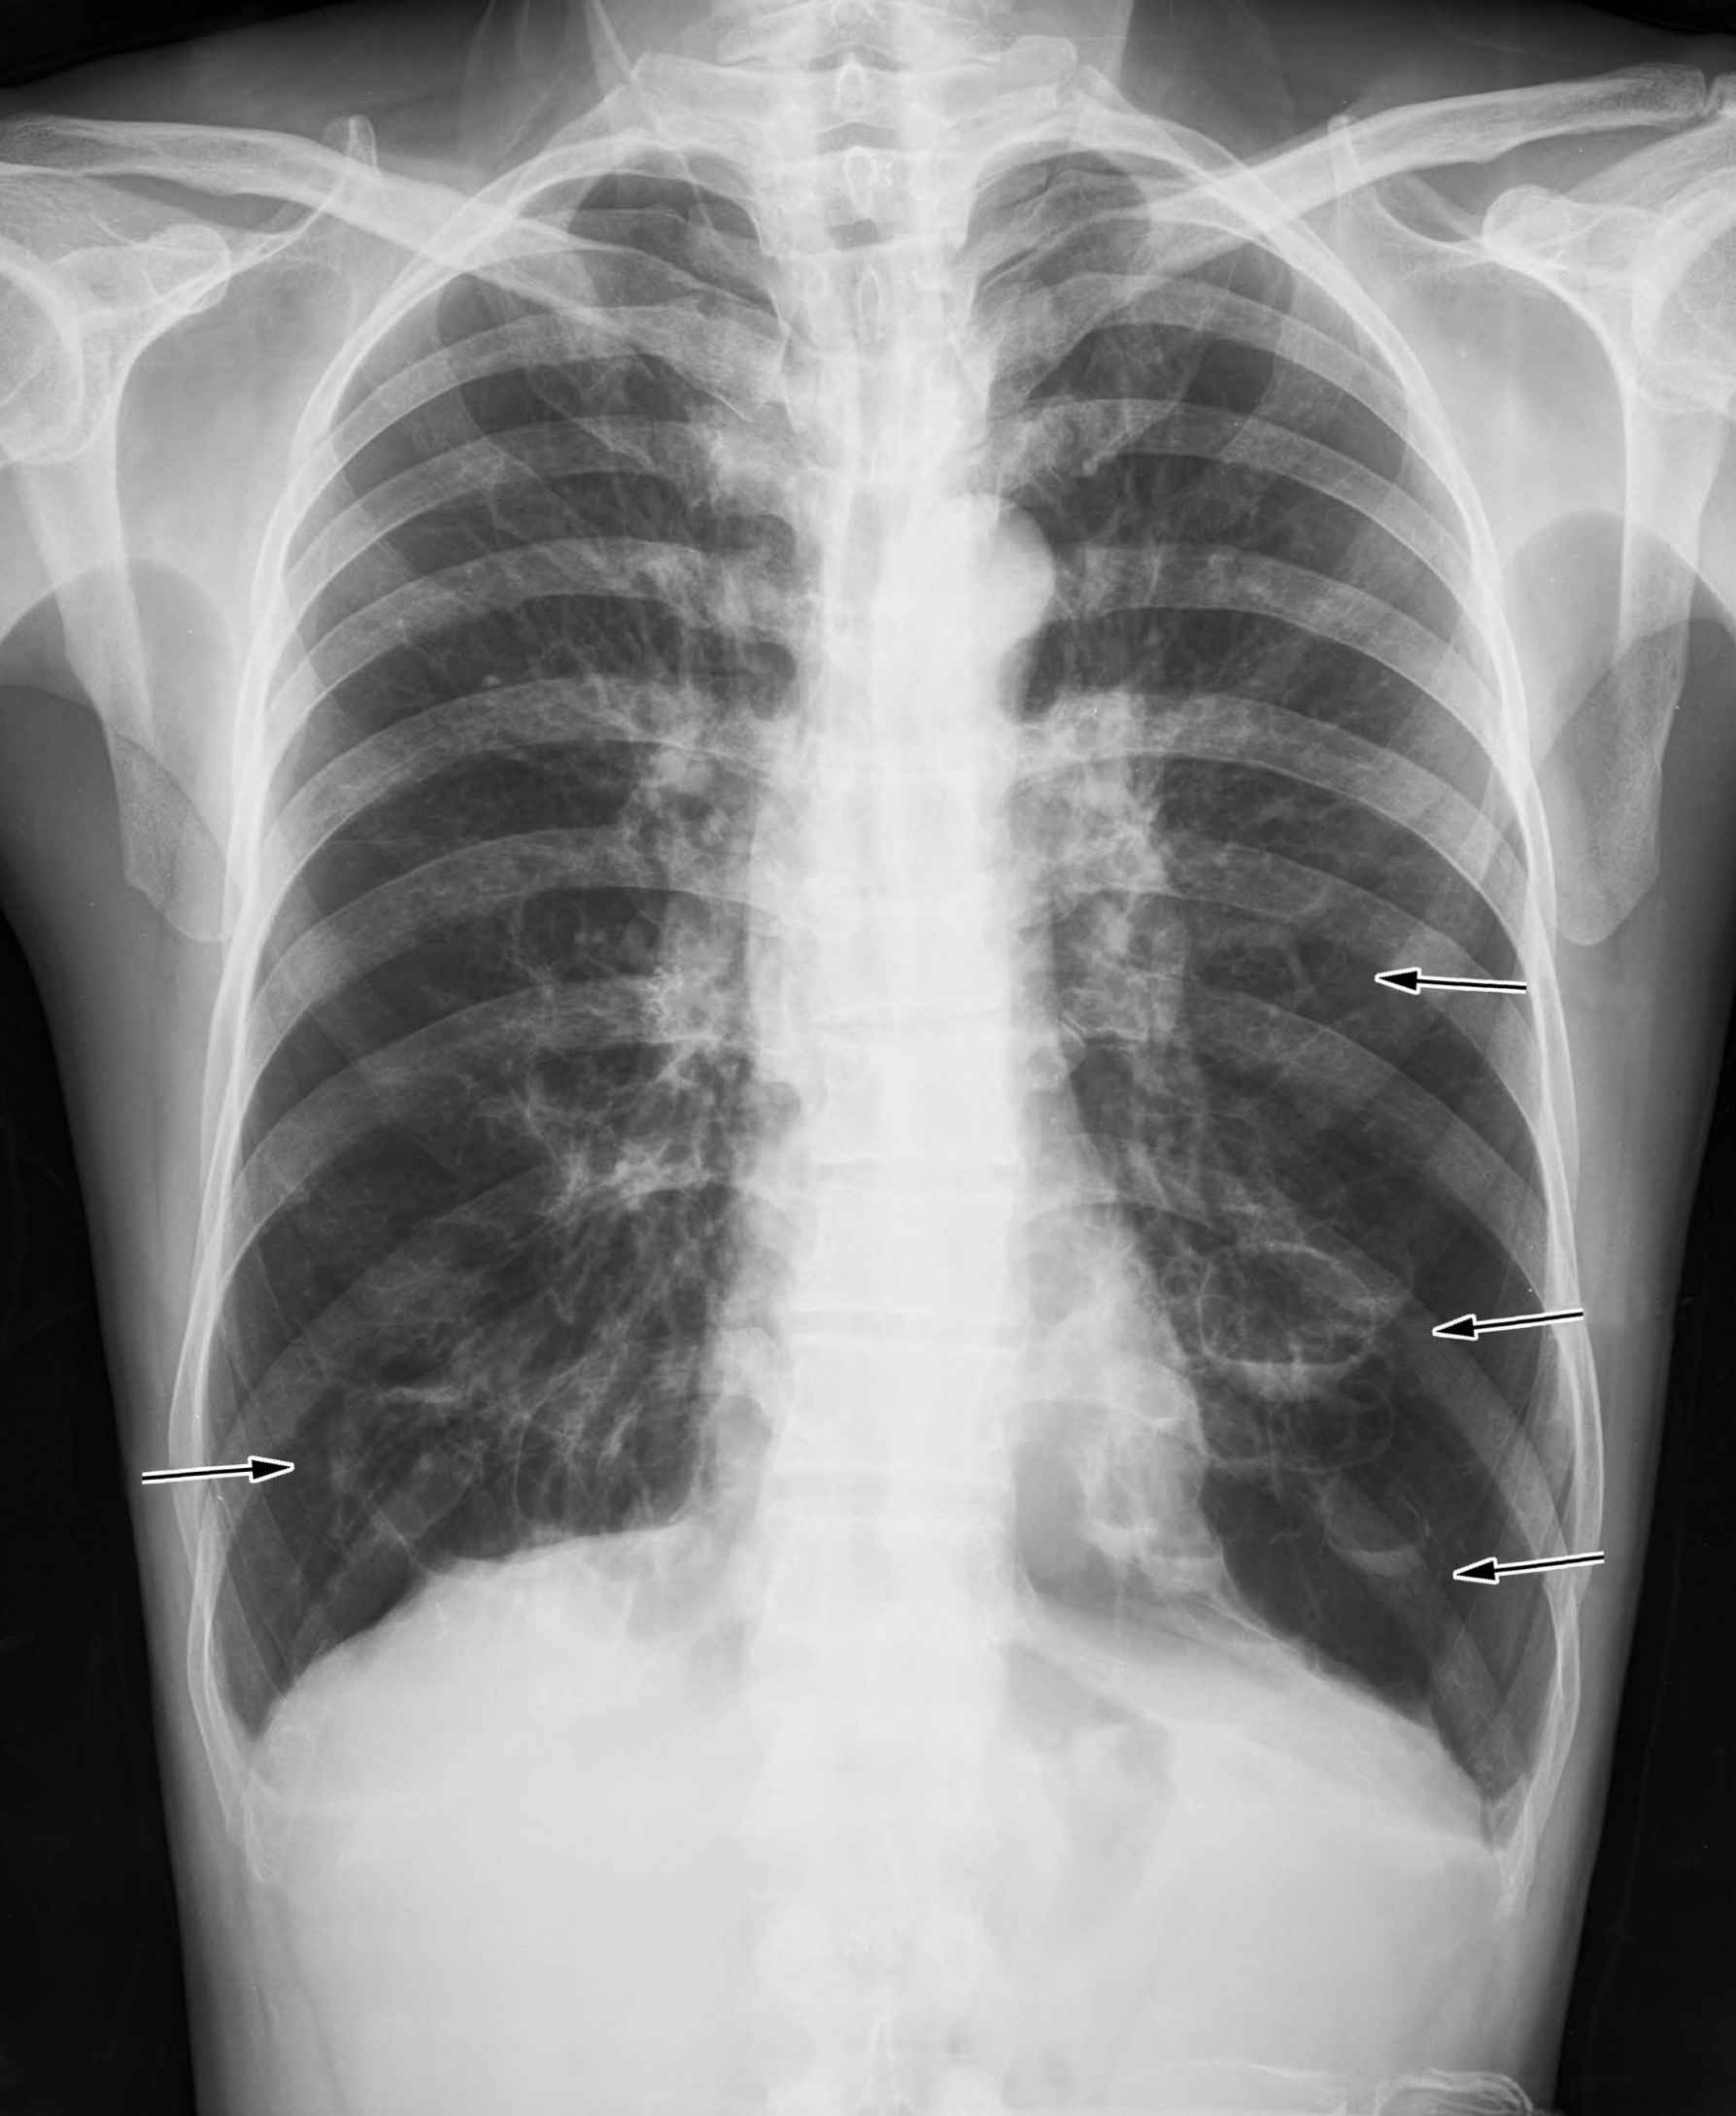
\includegraphics{./images/Image00138.jpg}
 \captionsetup{justification=centering}
 \caption{先天性支气管囊肿}
 \label{fig3-2-2}
  \end{figure} 

\textbf{【病史摘要】}
 男性,22岁。反复间断性咳嗽、咳痰10多年,近期加重。痰量时多时少,痰量多时常为脓痰。自诉患有“先天性支气管囊肿”。

\textbf{【X线表现】}
 双侧中下肺野见多枚卵圆形囊状透光区(箭头),壁较薄,多枚可见短小气液面,外壁尚光整,周围肺野尚清晰。两膈光整,肋膈角锐利。心影形态大小属正常范围。

\textbf{【X线诊断】}  两肺先天性支气管囊肿。

\textbf{【评  述】}
 先天性支气管囊肿是一种先天性疾病,与肺芽始基发育障碍有关,在胚胎发育时不能使原先为索状组织的支气管演变成中空的管状结构,远端支气管腔内的分泌物不能排出,可积聚膨胀,形成含液囊肿。根据发育障碍出现的早晚和部位,而决定囊肿为单发或多发。如不发育的索状部分已分支则可形成多发囊肿,尚未分支则形成孤立囊肿。当囊肿和周围支气管相通可成含气囊肿或液气囊肿。囊肿可位于纵隔、肺门或肺内,当肺胚芽尚在大气管附近异常发育时(即异常发育较早时),囊肿位于纵隔或肺门,称为支气管囊肿;而异常发育出现较晚者,异常胚芽易于停留在肺内,囊肿多位于肺内,称为肺囊肿。囊肿的囊壁一般薄而均匀,内层为上皮层,有支气管壁结构,可与后天性囊肿区别。囊内可为澄清液或血液。临床常见症状为咳嗽、咳痰、咯血、胸痛,感染时可发热、咳脓痰,囊肿小者可无症状。

含液支气管囊肿X线表现常呈圆形、卵圆形,或分叶状,边缘光滑锐利,周围肺组织清晰,密度均匀一致,出血者可钙化,有时囊壁可呈弧形钙化,呼吸气相囊肿大小形态可改变,邻近胸膜无改变;支气管含气囊肿和液气囊肿其囊内常存在液平,囊内有时有线样间隔,此时囊肿外形常呈分叶状,周围肺组织无卫星病灶,感染后囊壁增厚,可与急性肺脓肿相似,但抗感染治疗后可恢复囊肿原貌;反复感染者,囊壁纤维化,其表现与慢性肺脓肿不易区别;多发性支气管肺囊肿常可位于肺的一叶、一侧或双侧肺,以一侧者多见,可为多数薄壁环形透光区,如为无数大小不等的薄壁环形透光区相互重叠,占据整侧肺,状为蜂窝者,称为蜂窝肺或囊性肺,一般为气囊肿,但少数囊内可有较小的液平面,囊壁薄,边缘锐利,感染后囊壁可增厚而模糊,常有胸膜增厚。

先天性肺囊肿合并感染时,囊腔内可出现液平面,囊肿可因周围的炎性浸润或肺不张而加厚。此时需与肺脓肿鉴别。肺脓肿周围的炎性浸润比感染性肺囊肿厚,腔内液体一般较多,脓肿壁也较厚。急性肺脓肿治疗及时者完全吸收,先天性肺囊肿在感染吸收后囊壁不会消失。当囊肿与周围肺组织有粘连,使其形态成为不规则,特别在贴近胸膜处更明显,可成为密度浓密边缘清楚的阴影。累及胸膜时可致其增厚。临床上,先天性肺囊肿伴感染症状比较缓慢,无典型大量脓臭痰。有时尚需与包虫囊肿鉴别,尤其合并感染时更易混淆,根据患者的生活史及地区性,有助于鉴别。肺霉菌病所形成的空洞,如曲菌球,其特点为空洞内有致密圆形的游离球状体,在站立位及卧位比较可见其移动,痰中可找到大量霉菌。与孤立性液气囊肿鉴别不难。

先天性肺囊肿最难与囊状支气管扩张相鉴别。支气管扩张常为继发性病变,有慢性纤维增生性病变的后继病变,其病变严重程度与纤维增生成比例增加,因此支气管扩张患者局部肺纹理常增多、增粗且紊乱,囊壁相对较厚且不甚光整;而肺囊肿一般为先天性病变,虽常伴感染,但其囊肿壁薄而均匀,囊内张力一般较大,病变周围出现肺纹理增多紊乱的程度不如囊状支气管扩张。另外,囊状支气管扩张常有特征性的卷发样改变、印戒征、轨道征等征象,可与肺囊肿相鉴别。

\subsection{急性支气管炎}

\begin{figure}[!htbp]
 \centering
 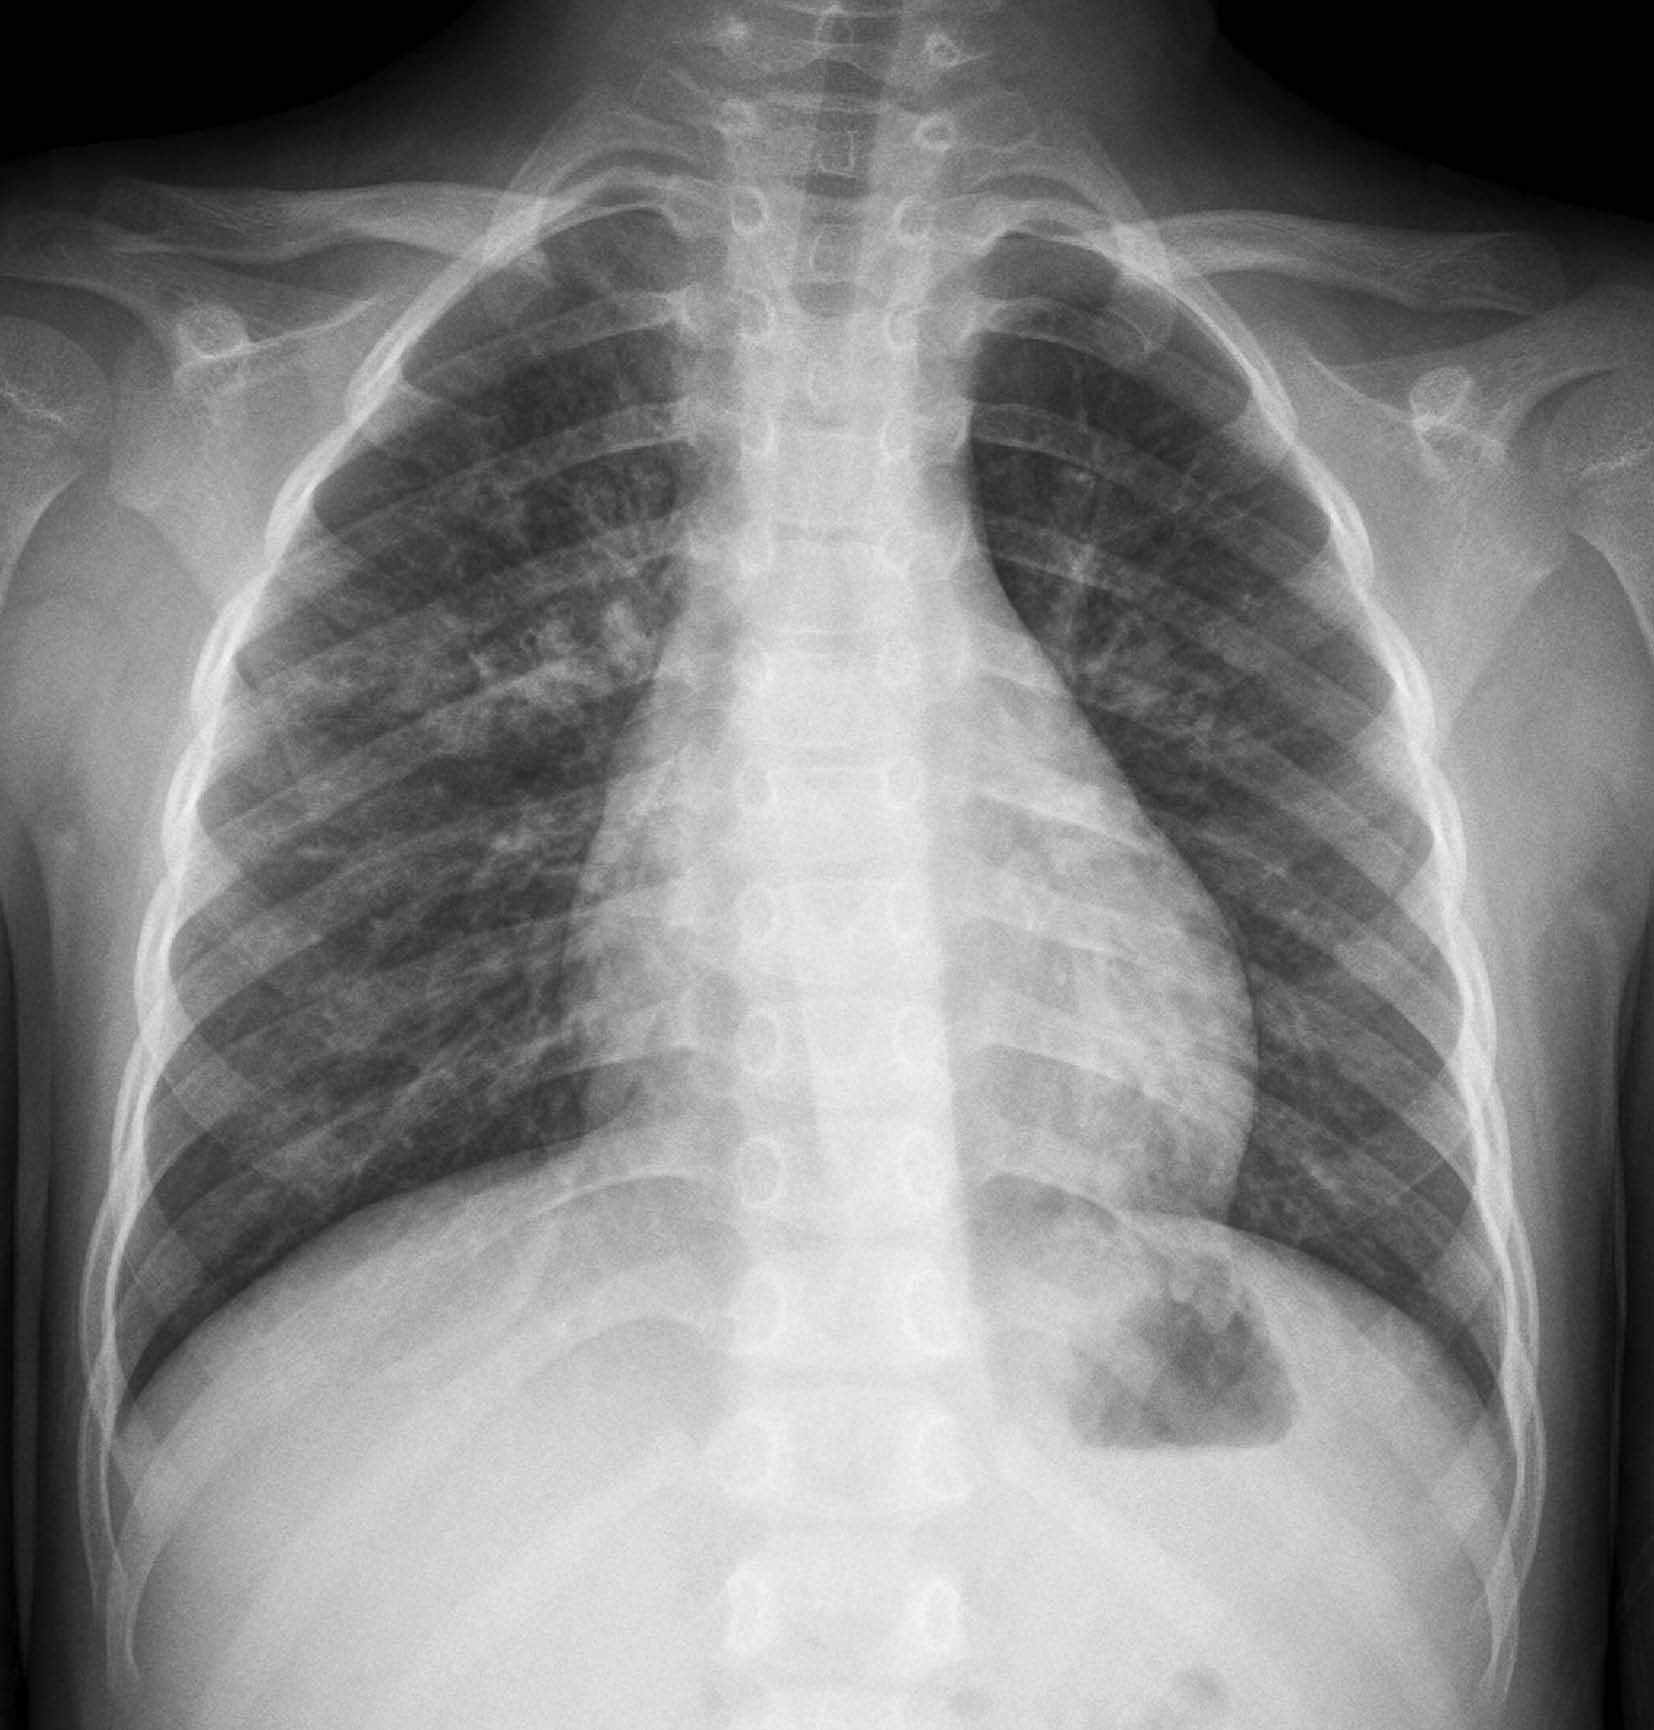
\includegraphics{./images/Image00139.jpg}
 \captionsetup{justification=centering}
 \caption{急性支气管炎}
 \label{fig3-2-3}
  \end{figure} 

\textbf{【病史摘要】}  女性,6岁。鼻塞流涕、咳嗽、咳粘痰2天,发热1天。

\textbf{【X线表现】}
 两肺纹理增多、增粗,以右侧明显,右肺野纹理模糊。两膈光整,肋膈角锐利;心影形态大小属正常范围。

\textbf{【X线诊断】}  X表现并结合临床符合急性支气管炎。

\textbf{【评  述】}
 急性支气管炎是病毒或细菌等病原体感染所致的支气管粘膜炎症。是婴幼儿时期的常见病、多发病,往往继发于上呼吸道感染之后,也常为肺炎的早期表现。本病多同时累及气管、支气管,故正确命名应为急性气管支气管炎。临床以咳嗽伴(或不伴)有支气管分泌物增多为特征,一般起病前有上呼吸道感染的症状,鼻塞、喷嚏、声音嘶哑、全身不适,部分患者有畏寒、发热、全身肌肉酸痛、咳嗽、咳痰、痰量逐渐增多,痰为粘液样或粘液脓性痰。

粘膜充血是急性支气管炎的早期病理改变,接着出现脱屑、水肿、粘膜下层白细胞浸润和粘稠或粘液脓性分泌物产生,支气管纤毛、巨噬细胞和淋巴管的防御功能障碍。细菌得以侵犯正常时无菌的支气管,继而细胞碎片以及粘液脓性分泌物积聚。咳嗽对于排除支气管分泌物是必需的。支气管壁水肿,分泌物潴留以及某些患者的支气管平滑肌痉挛,可致气道阻塞。

急性支气管炎的X线胸片或胸部透视一般显示正常或仅有肺纹理增多、增粗及模糊征象,无明确诊断意义。因肺纹理的粗细、多少等缺少绝对评价标准,故判断肺纹理的改变,必须慎重,确实明显增多、增粗,才可描述,此时患者临床上有急性支气管炎症状,如喉痒、咳嗽、咳白色粘痰或少许黄色粘痰,重症可合并发热,方可诊断为急性支气管炎。

许多情况下,摄X线胸片的目的不是诊断支气管炎而是有无并发肺部炎症,或由粘痰所引起的气道阻塞改变,如局部肺气肿或肺不张等。

\subsection{慢性支气管炎}

\begin{figure}[!htbp]
 \centering
 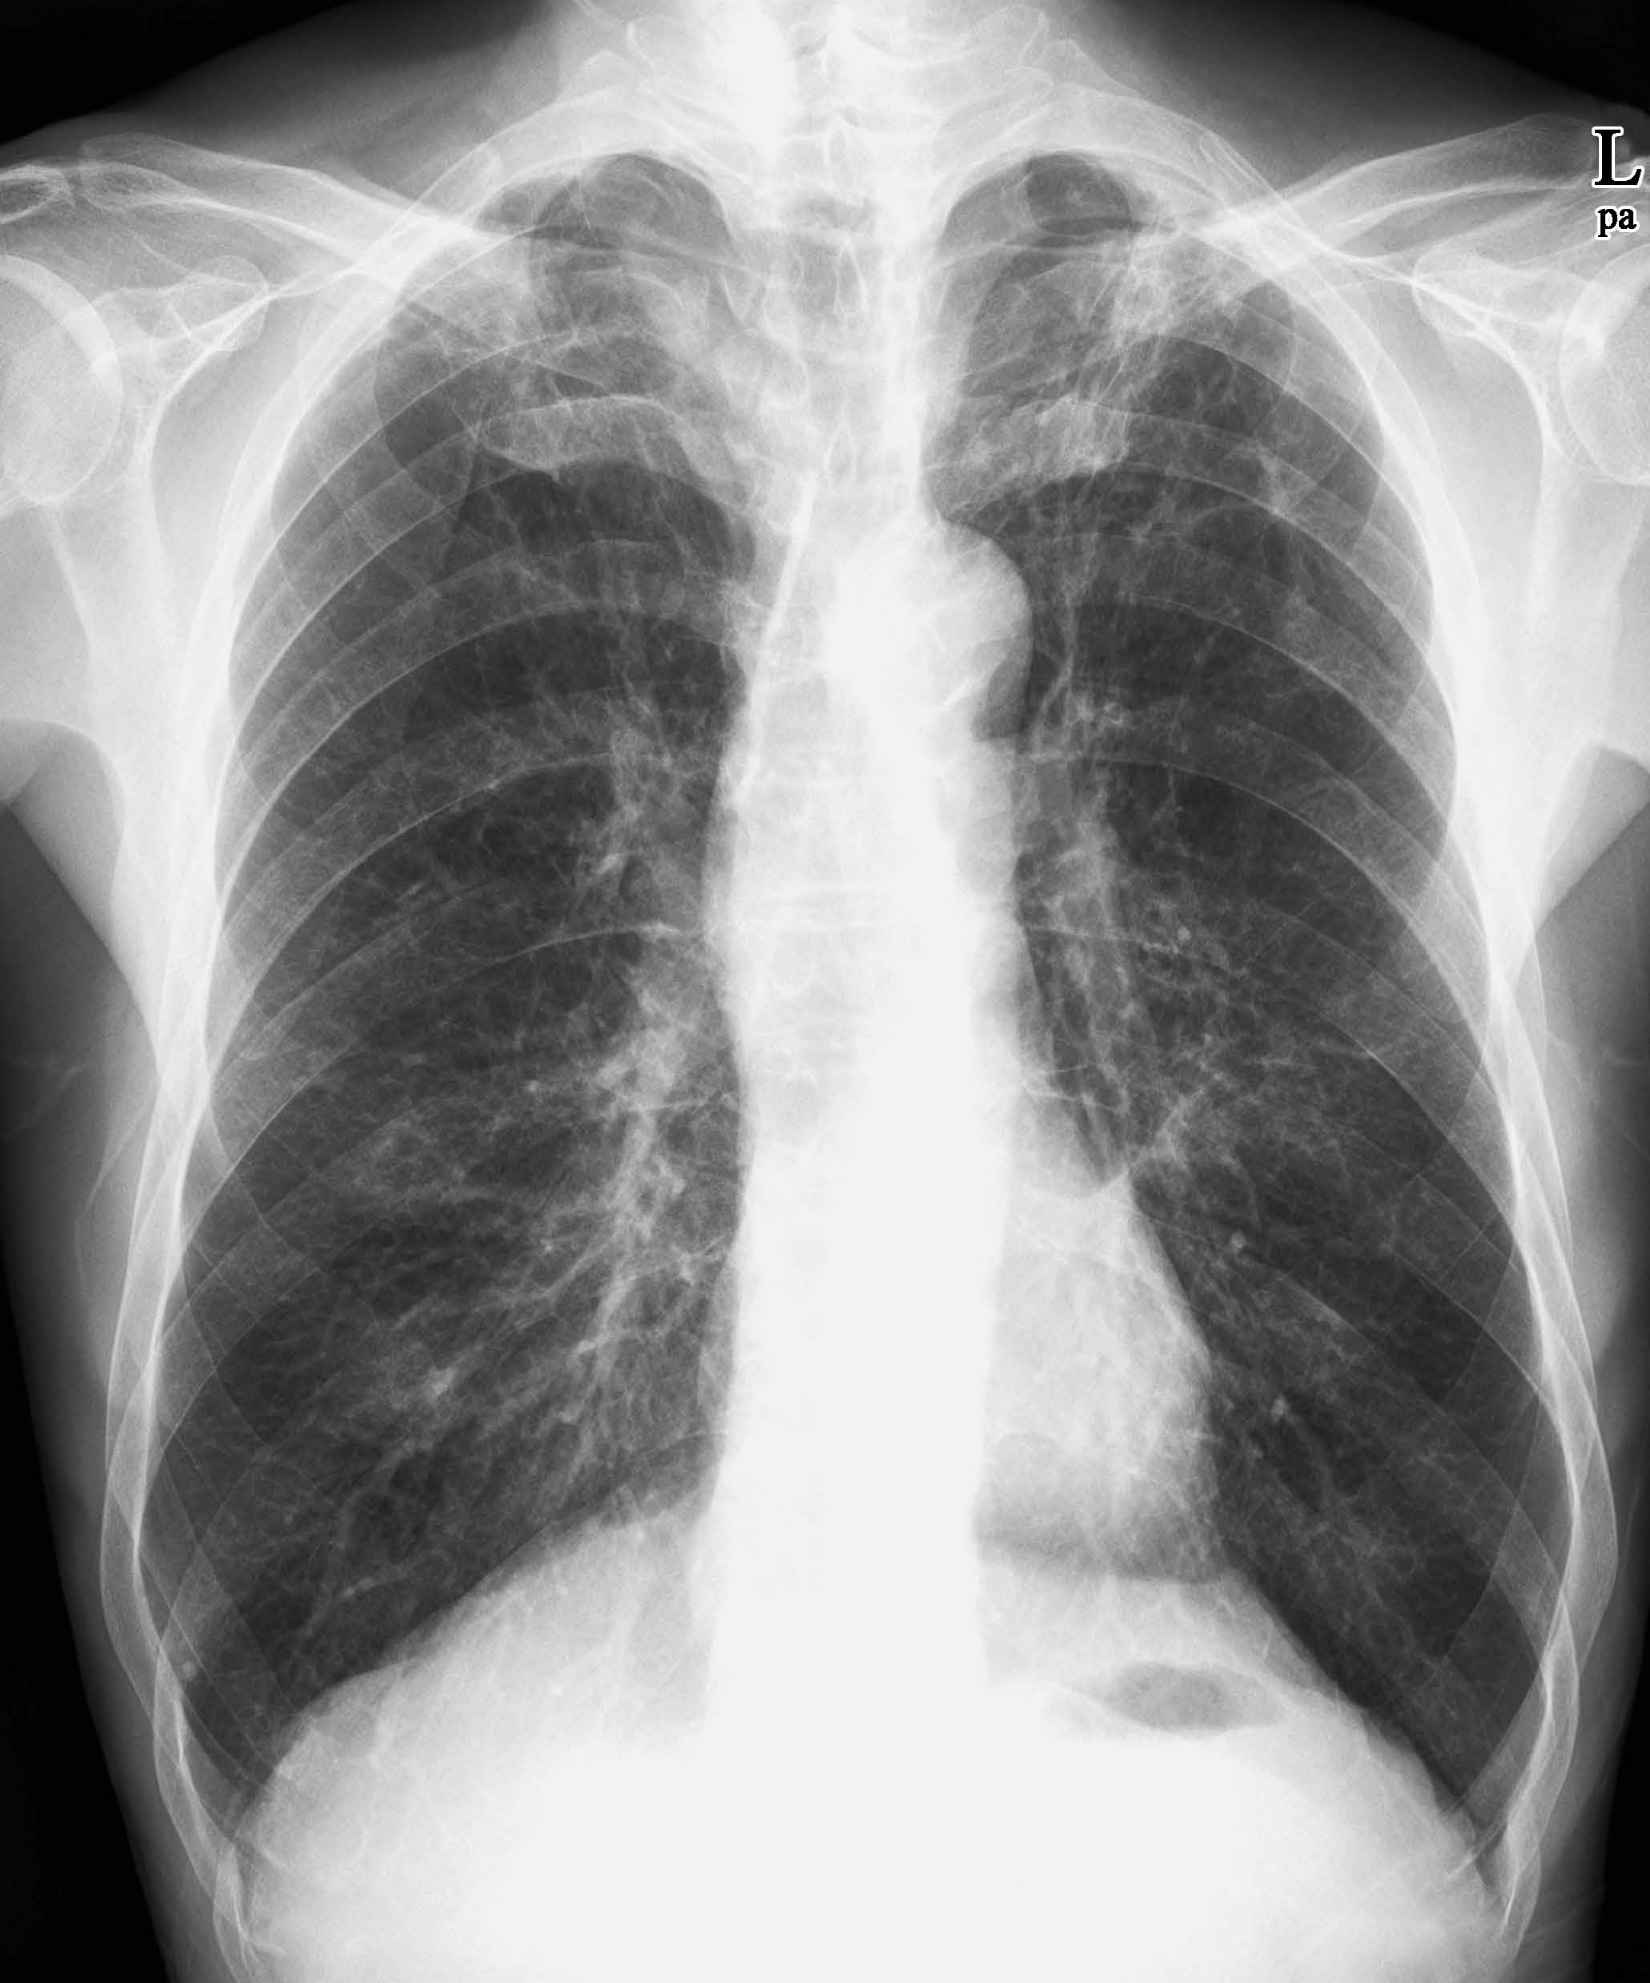
\includegraphics{./images/Image00140.jpg}
 \captionsetup{justification=centering}
 \caption{两肺慢性支气管炎伴肺气肿}
 \label{fig3-2-4}
  \end{figure} 

\textbf{【病史摘要】}
 男性,67岁。反复咳嗽、咳痰伴有时气喘10多年,加重3天。

\textbf{【X线表现】}
 肋骨轻度平举,胸廓略成桶状。肺门影明显增宽,肺纹理增多紊乱,肺野透光度增强。两膈位置降低,心影呈滴状。

\textbf{【X线诊断】}  两肺慢性支气管炎伴肺气肿。

\textbf{【评  述】}
 慢性支气管炎是指气管、支气管、粘膜及周围组织的慢性非特异性炎症。随着病程的迁延和发展,大多数患者可并发慢性阻塞性肺气肿、肺大疱形成,肺间质纤维化,甚至可导致肺源性心脏病。临床上以咳嗽、咳痰、气喘为主要症状。可闻及哮鸣音。后期出现气短,待发生肺源性心脏病时,则气急加重,甚至有发绀及颈静脉怒张等征象。

X线平片表现:两肺纹理普遍增粗、增多,呈粗细不均、排列不齐、交错紊乱的索条影,有时伴有支气管扩张的改变。在右下肺心缘旁有时可见轨道征,在支气管走行部位可见到互相平行的线状阴影,为增厚的支气管壁,其间的透光带为支气管腔。气管胸段冠状径较小,矢状径增宽,形如刀鞘状,称刀鞘状气管,发生机制是因用力咳嗽及呼吸,使气管内压力增加,在气管壁炎症的基础上而引起刀鞘状变形。老年性慢性支气管炎的患者,常伴有弥漫性肺气肿,胸廓桶状,两肺透亮度增高,横膈面低平,呼吸运动幅度降低,心影狭长,甚至出现肺大疱,肺血量减少使肺纹理显著稀少而纤细。肺心病亦是常见的并发症,表现为肺门影明显增宽而外围血管相对变细,肺动脉段突出或基线延长,右心室肥厚扩大。

慢性支气管炎的临床诊断标准:慢性进行性咳嗽、咳痰,每年至少3个月,连续两年以上。并除外全身性或肺部其他疾病。冬季发病较多,易发生急性呼吸道感染。

慢性支气管炎是常见的老年呼吸系统疾病,常伴发感染,并发肺大疱、肺气肿。X线检查简便快捷,同时可监测病程发展,及时发现并发症。

\subsection{支气管扩张(一)}

\begin{figure}[!htbp]
 \centering
 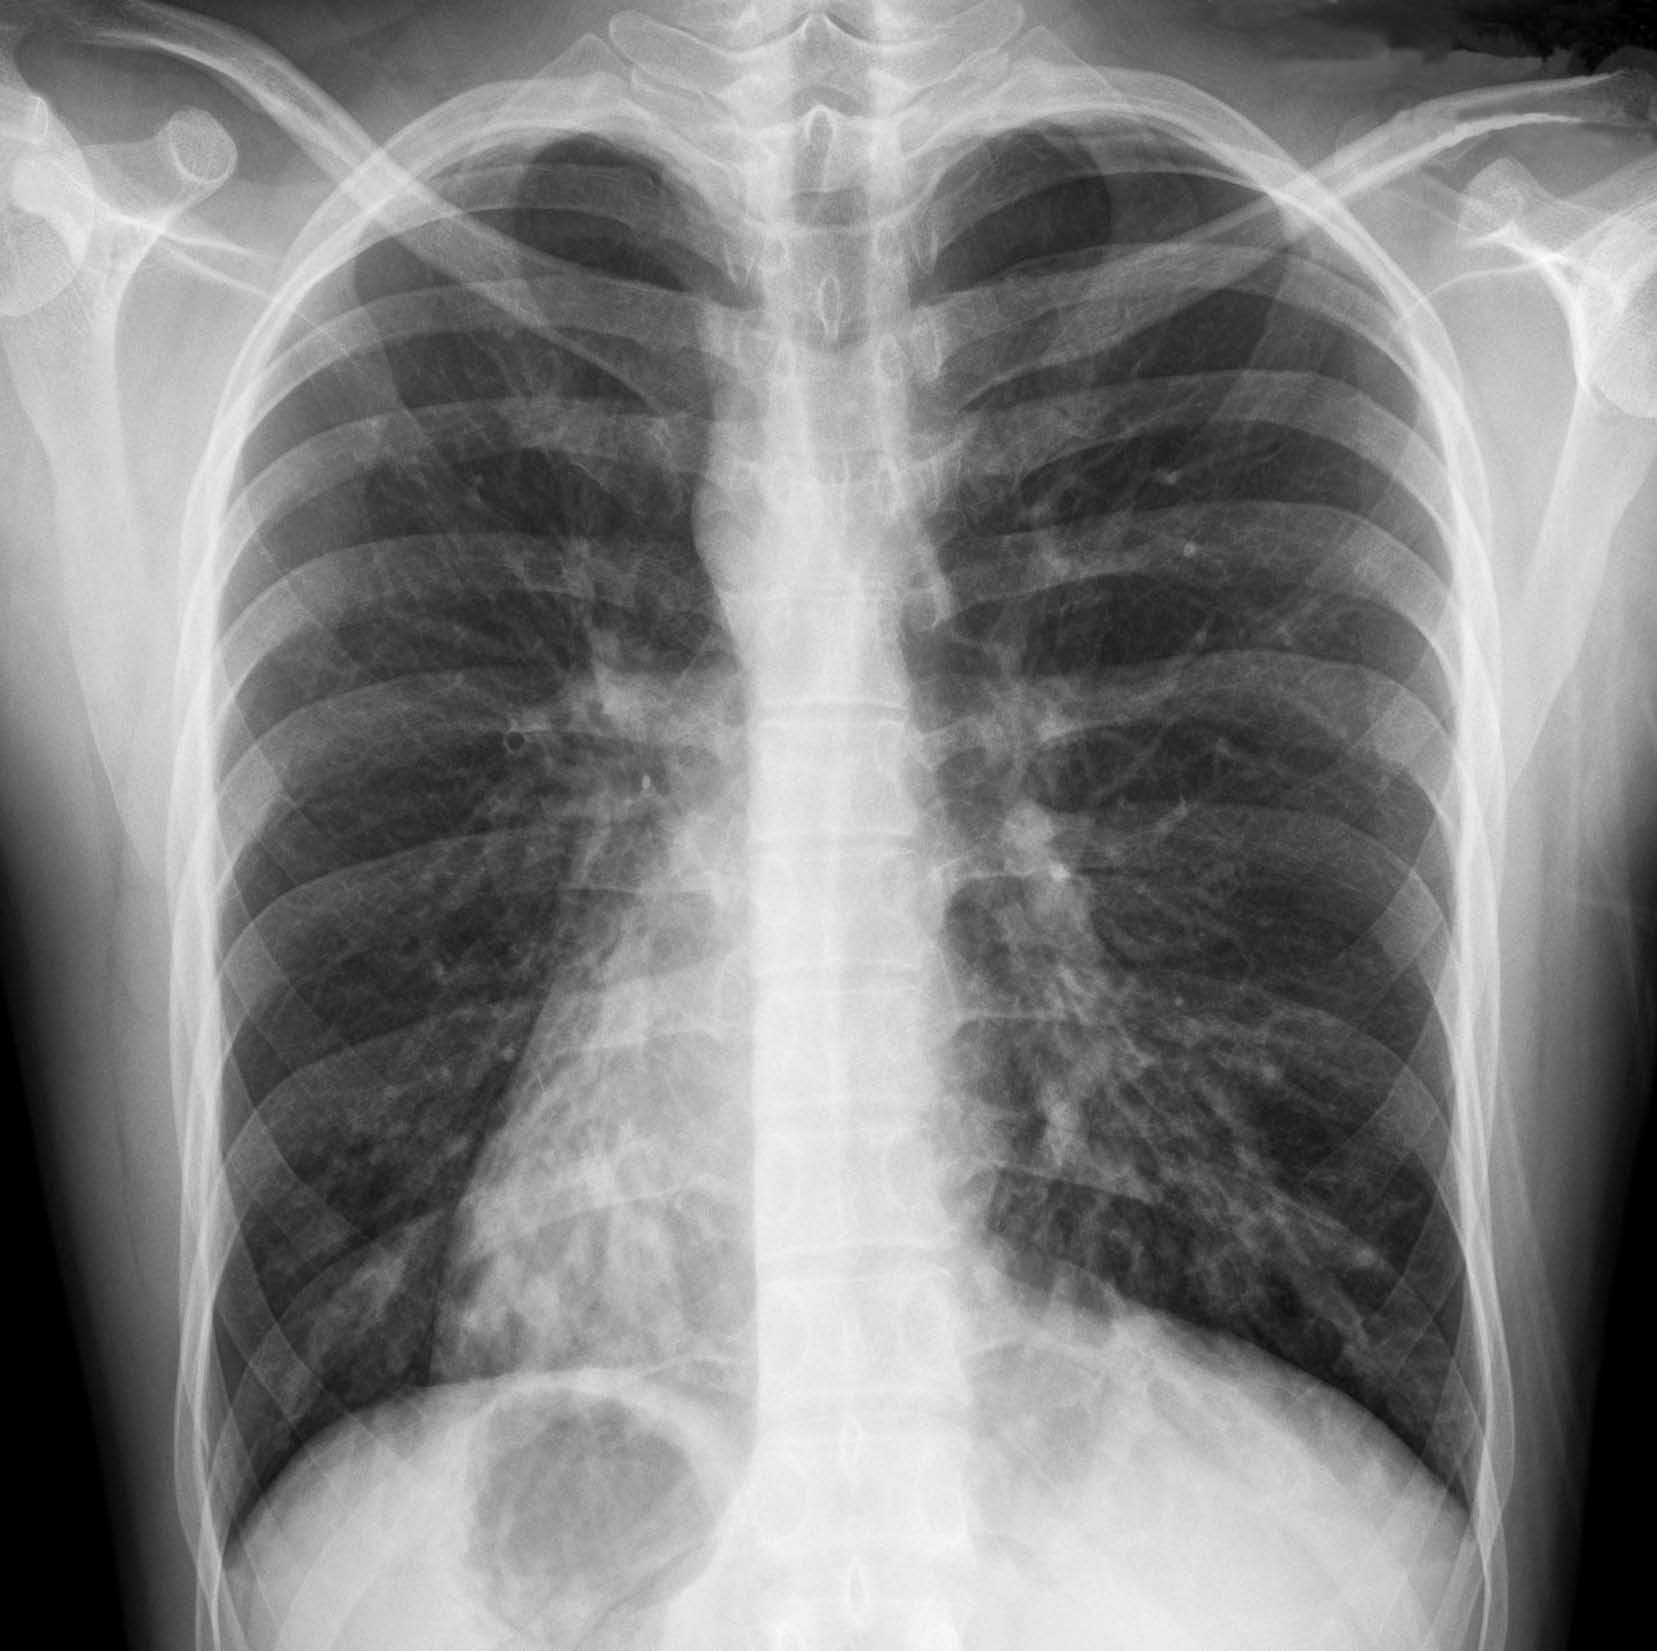
\includegraphics{./images/Image00141.jpg}
 \captionsetup{justification=centering}
 \caption{两下肺支气管柱状扩张}
 \label{fig3-2-5}
  \end{figure} 

\textbf{【病史摘要】}  男性,23岁。咳嗽、咳痰、咯血1周。

\textbf{【X线表现】}
 两肺纹理增多、增粗、紊乱,两下肺见柱状扩张支气管影,以左侧明显,远端扩张,呈杵状及双轨状影,周围纹理边缘模糊。左膈高于右膈,心尖及心影大部位于中线右侧,心影形态大小无明显异常,胃泡位于右侧膈下,此例患者有全内脏反位先天变异。

\textbf{【X线诊断】}  左下肺柱状支气管扩张。全内脏反位。

\textbf{【评  述】}
 支气管扩张分为先天性或后天性两种,前者少见,有些病例伴内脏反位;后者较常见,男女发病无明显差异,好发于儿童及青壮年。临床上以慢性咳嗽、咯大量脓痰和反复咯血为三大主要症状,感染时可发热,少数患者仅有咯血。

后天性支气管扩张的主要发病机制是:慢性感染引起支气管壁组织的破坏;支气管内分泌物淤积与长期剧烈咳嗽,引起支气管内压增高;肺不张及肺纤维化对支气管壁产生的外在性牵拉。这三个因素互为因果,促成并加剧支气管扩张。先天性支气管扩张病理改变为管壁平滑肌、腺体和软骨减少或缺如,同时有支气管上皮脱落,支气管壁内炎性细胞浸润,管壁肿胀和周围纤维组织增生。支气管扩张一般发生在3~6级分支,根据形态可分为:柱状型、曲张型、囊状型支气管扩张。三种类型可同时混合存在或以其中一种形态为主出现。支气管扩张可两肺同时存在,两肺呈广泛者较少见,尤以右肺下叶、左肺下叶和左肺舌叶多见。

胸部X线平片肺部常可无异常发现(有10%左右),有时仅有肺纹增多、粗乱,出现双轨阴影时与慢性支气管炎相似,如见管径明显增粗的双轨影或杵状阴影,邻近可有肺气肿及胸膜增厚,对诊断有很大帮助;当支气管扩张肺部有继发感染时表现为肺实质炎,呈现为肺的某一个局部见多数小斑片状密度增高影,边缘模糊,且在同一个区域反复出现;有时可伴有肺不张,这些征象可提示支气管扩张可能,但缺少特征性。但当在粗乱的肺纹理中见到杵状、管状透光影,或囊状、蜂窝状阴影,有时呈卷发状阴影时,此为支气管扩张较为特征的表现。

当中青年患者有咯血或反复肺部感染的病史,X线平片见两下肺片状阴影不易吸收,肺纹理明显增粗,特别是有多发环状阴影时提示本病的可能性。有时需与多发性肺囊肿鉴别,前者壁稍厚,且不规则,局部肺纹理增粗、紊乱;后者壁较薄,稍光滑。CT检查可提供更多鉴别诊断信息。

\subsection{支气管扩张(二)}

\begin{figure}
  \centering
\subfloat[X线正位胸片]{
\begin{minipage}[b]{0.7\textwidth}
\centering
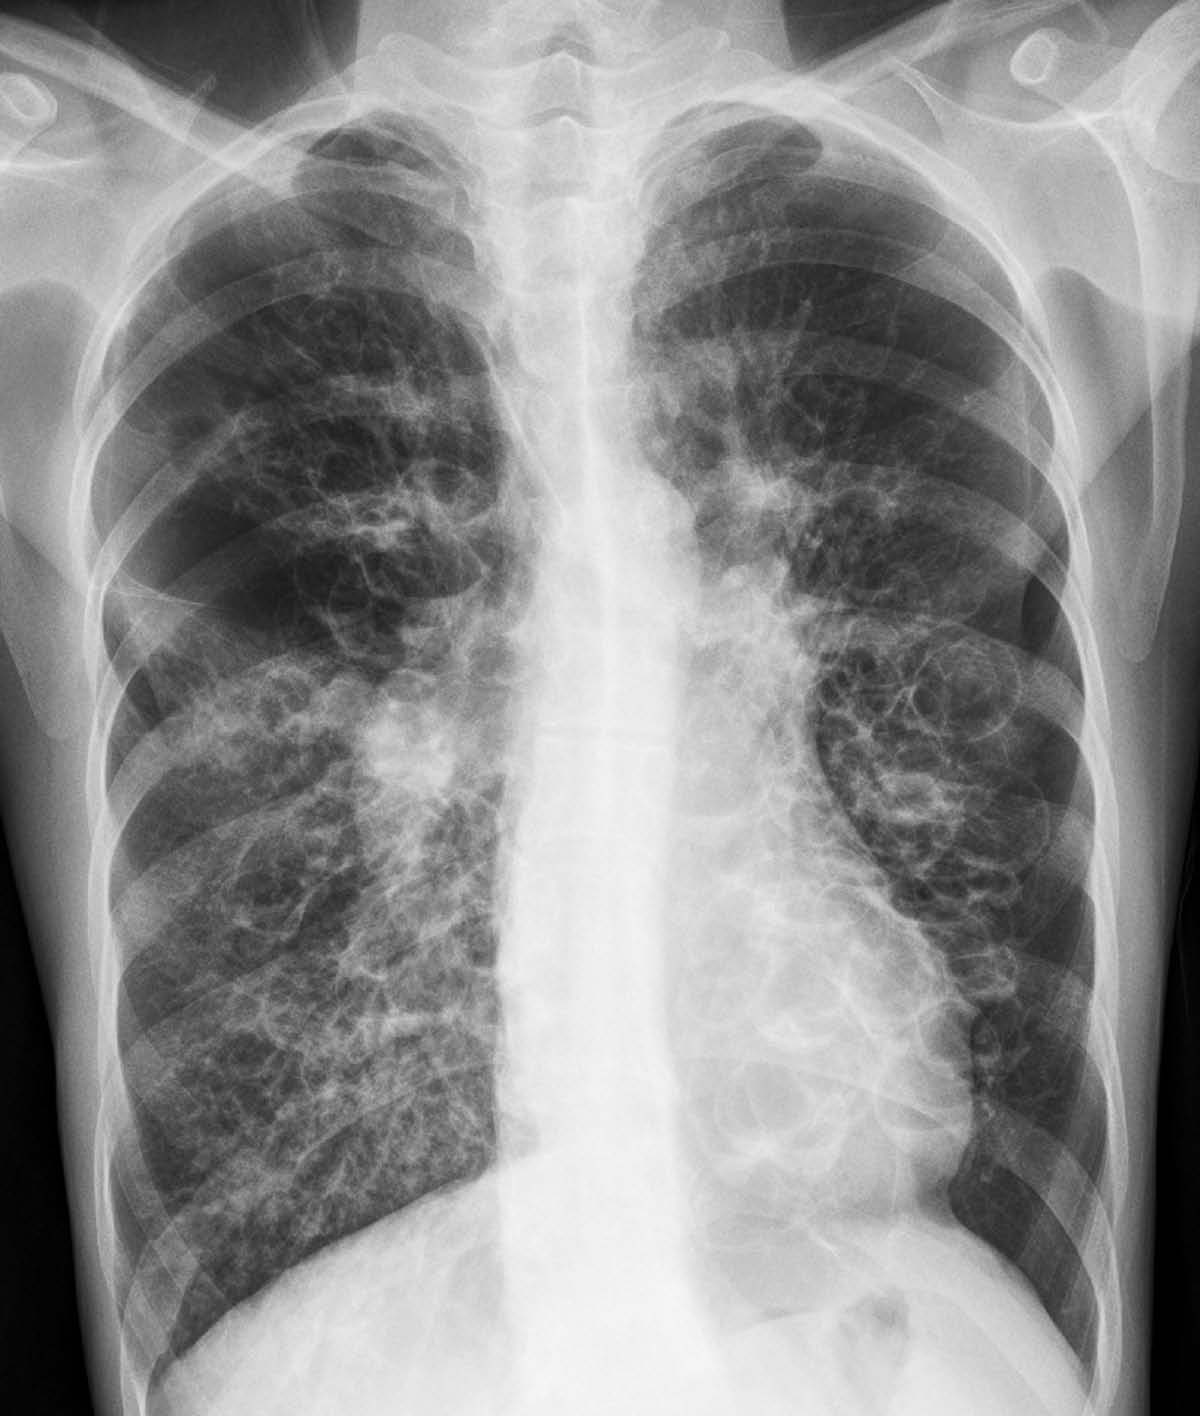
\includegraphics{./images/Image00142.jpg}
\end{minipage}}\\
\subfloat[(CT肺窗)两肺支气管囊状扩张]{
\begin{minipage}[b]{0.7\textwidth}
\centering
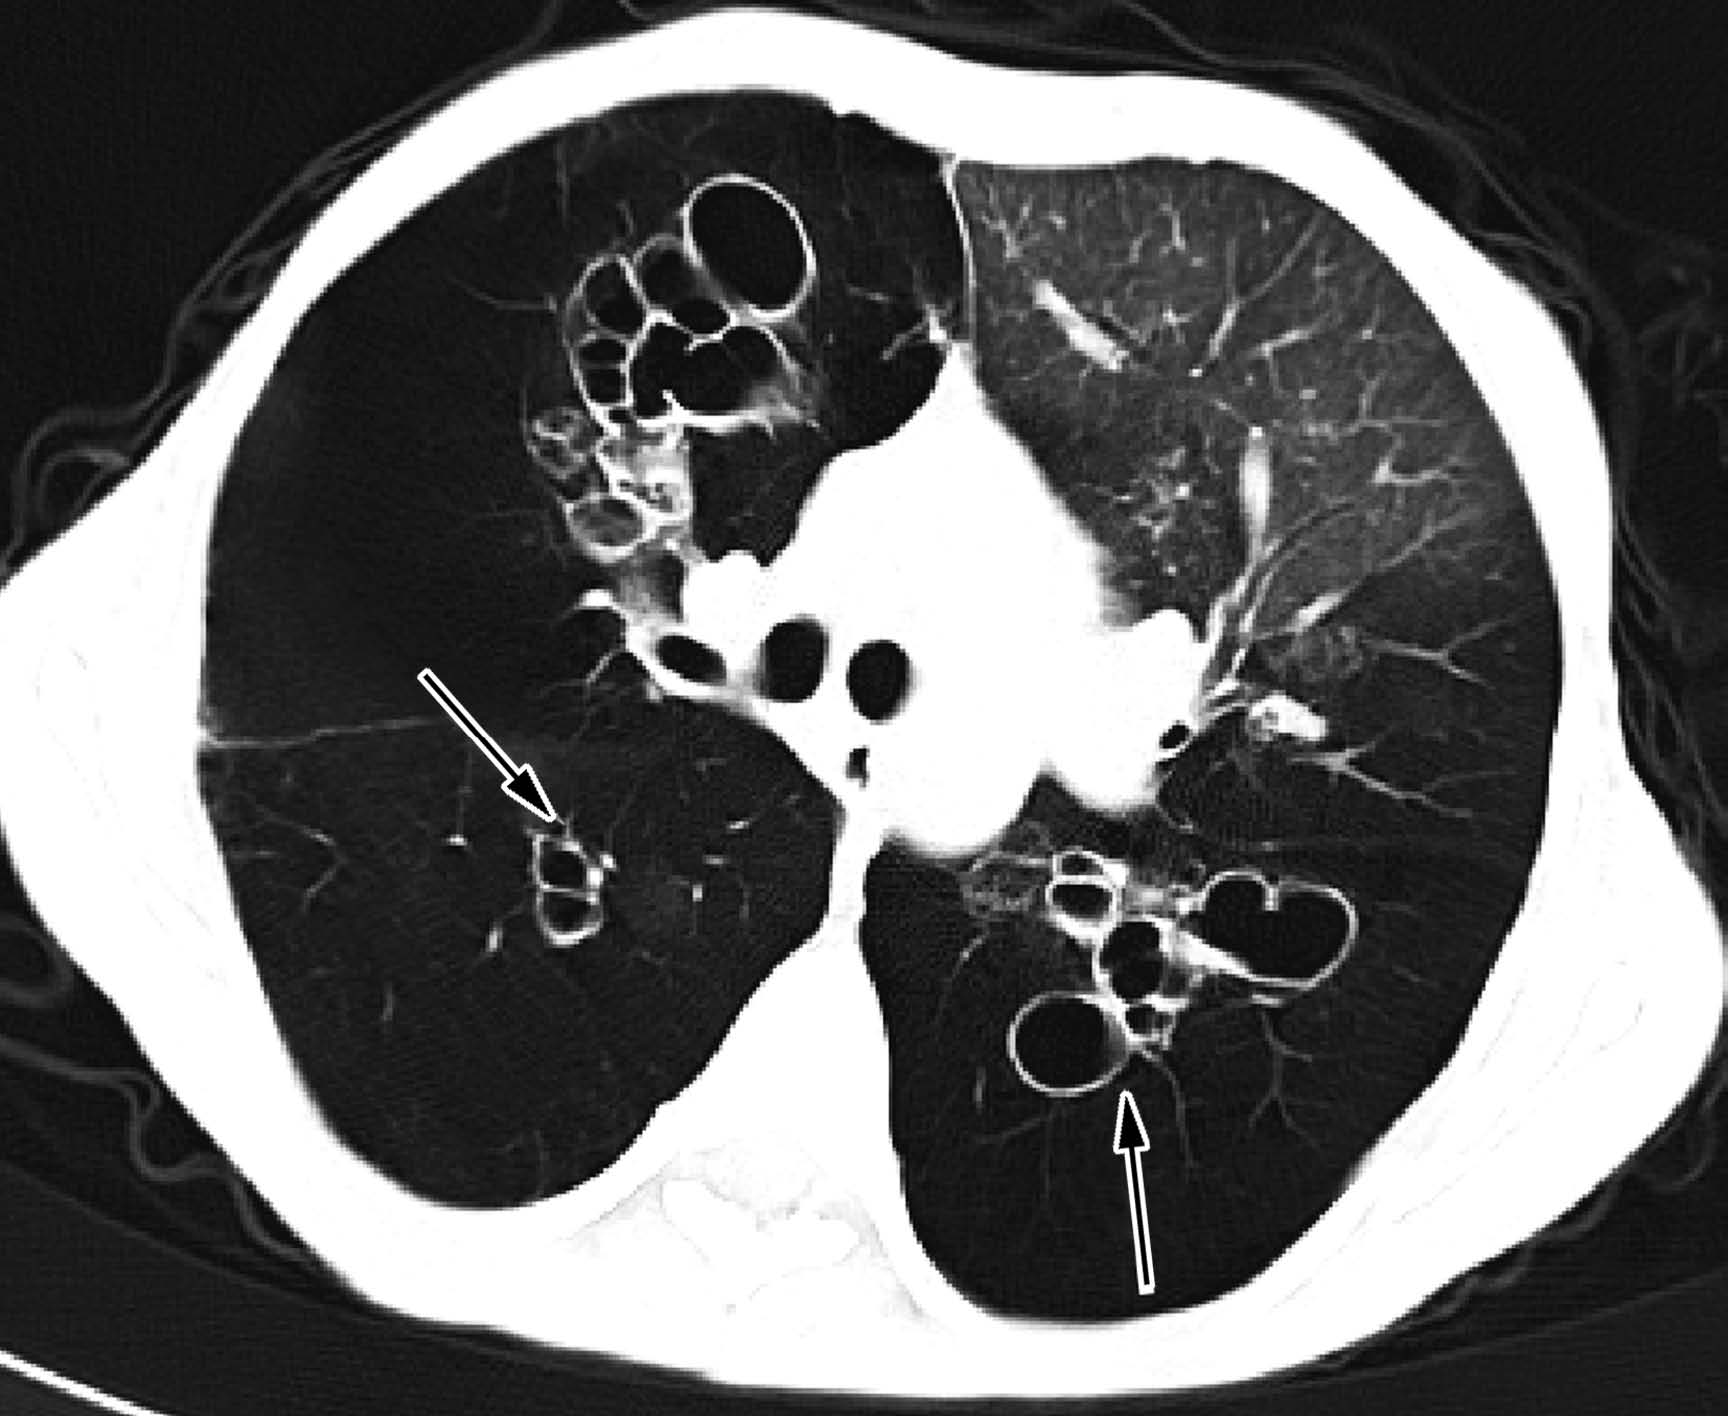
\includegraphics{./images/Image00143.jpg}
\end{minipage}}\\
\caption{}
\label{fig3-2-6}
\end{figure}

\textbf{【病史摘要】}
 女性,41岁。反复咳嗽、咳大量黄脓痰30年,气喘10年,加重5天。

\textbf{【X线表现】}
 两肺纹理稀疏紊乱,部分肺野透亮度增高,肺野增大;双侧肺野内、中带见多发囊状、蜂窝状阴影,局部呈卷发状改变,囊壁薄而均匀,外缘尚清,部分囊状影中见短小液平。右下肺动脉影明显增宽,肺动脉段突出,心影不大,心尖上翘,心轴向左后旋。同一患者CT肺窗显示支气管囊状扩张影,呈葡萄串状,可见戒指征(箭头)。

\textbf{【X线诊断】}  两肺支气管囊状扩张;两肺肺气肿;肺动脉高压。

\textbf{【评  述】}
 对于支气管扩张的影像诊断,目前常规X线检查仅作为初选,确定支气管扩张的存在、类型和范围以往主要依靠支气管碘油造影,但患者需忍受较大的痛苦,现已渐渐淘汰。目前主要依靠高分辨力CT,其主要CT表现为:正常时支气管管径相当于或略小于其伴随肺动脉管径,当支气管管径大于其伴随肺动脉管径时,应怀疑支气管扩张的存在。柱状型支气管扩张时,当支气管水平走行而与CT层面平行时可表现为轨道征;当支气管和CT层面呈垂直走行时可表现为管壁圆形透亮影,呈戒指征。囊状型支气管扩张时,支气管远端呈囊状膨大,成簇的囊状扩张可形成葡萄串状阴影,合并感染时囊内可出现液平及囊壁增厚。曲张型支气管扩张可表现支气管径呈粗细不均的囊柱状改变,壁不规则,可呈念珠状。当扩张的支气管腔内充满粘液栓时,表现为柱状或结节状高密度阴影,类似指状征改变。

\section{肺先天性疾病}

\subsection{肺隔离症}

\begin{figure}
  \centering
\subfloat[X线正位胸片]{
\begin{minipage}[b]{0.7\textwidth}
\centering
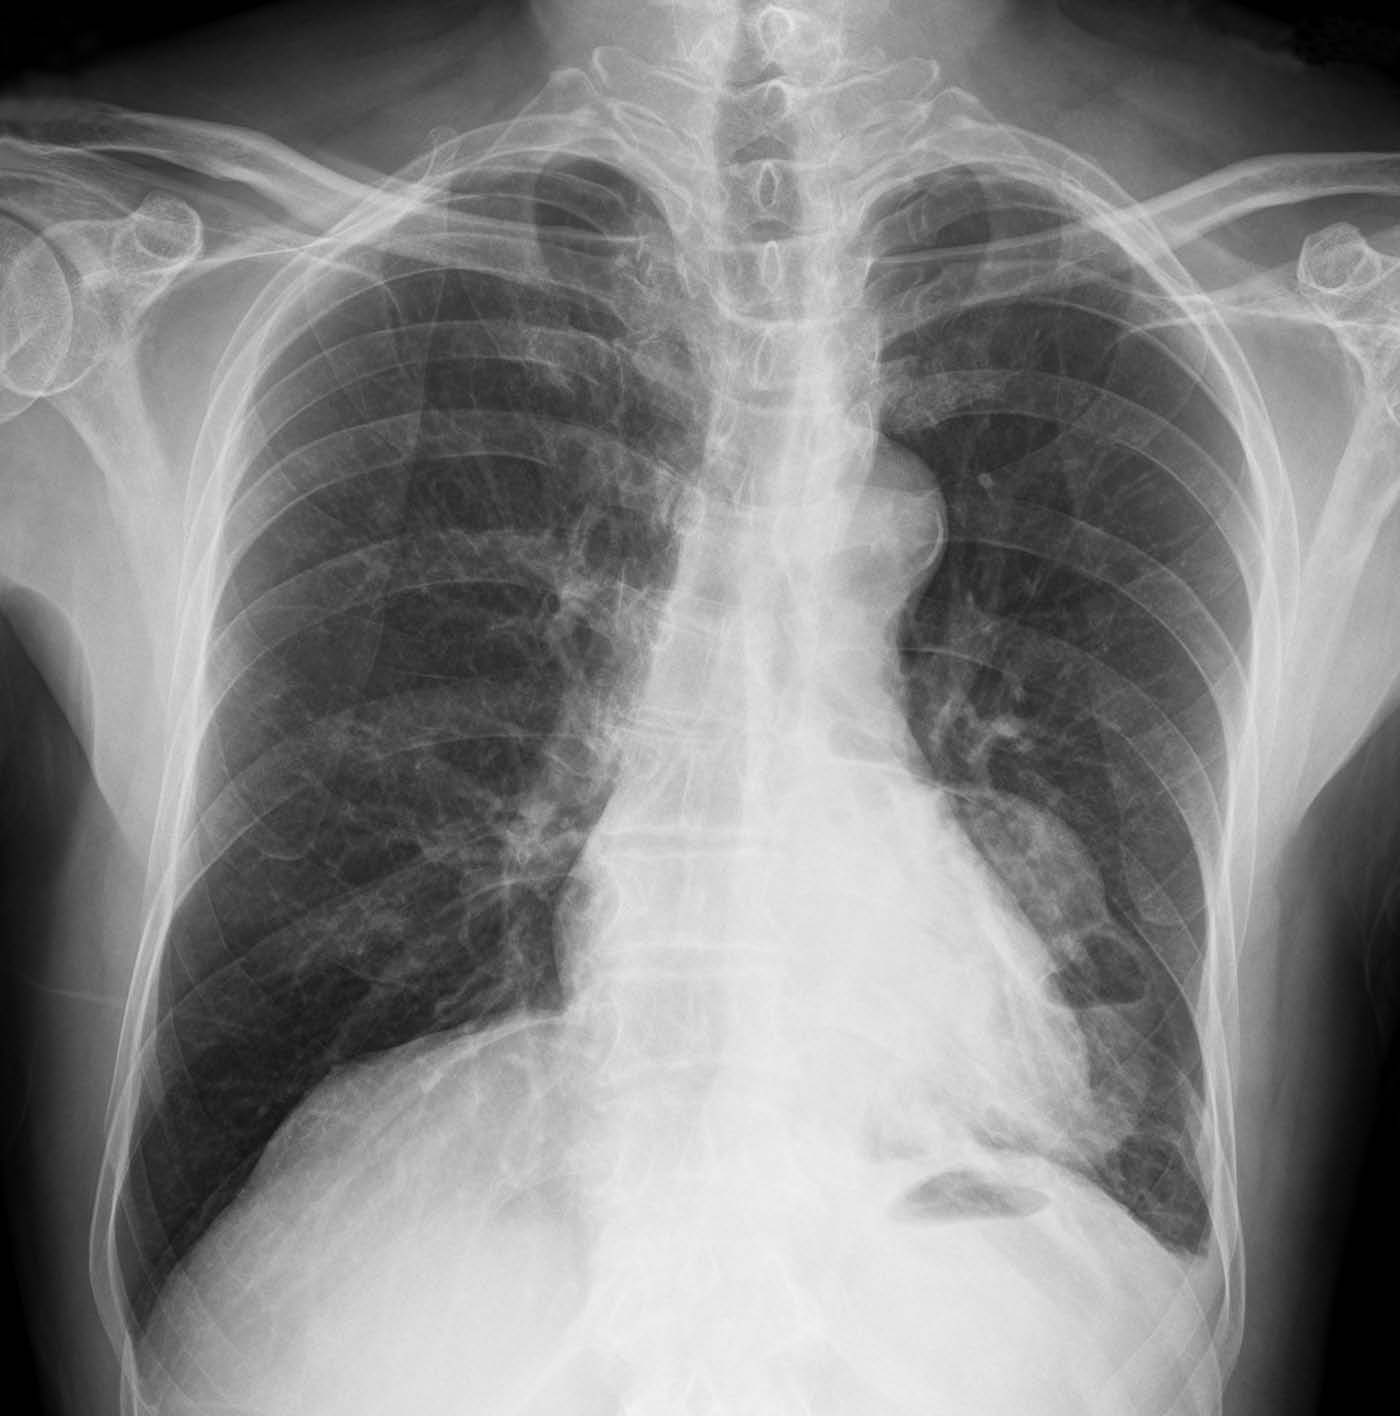
\includegraphics{./images/Image00144.jpg}
\end{minipage}}\\
\subfloat[胸部主动脉CT血管造影薄层最大密度投影冠状位]{
\begin{minipage}[b]{0.7\textwidth}
\centering
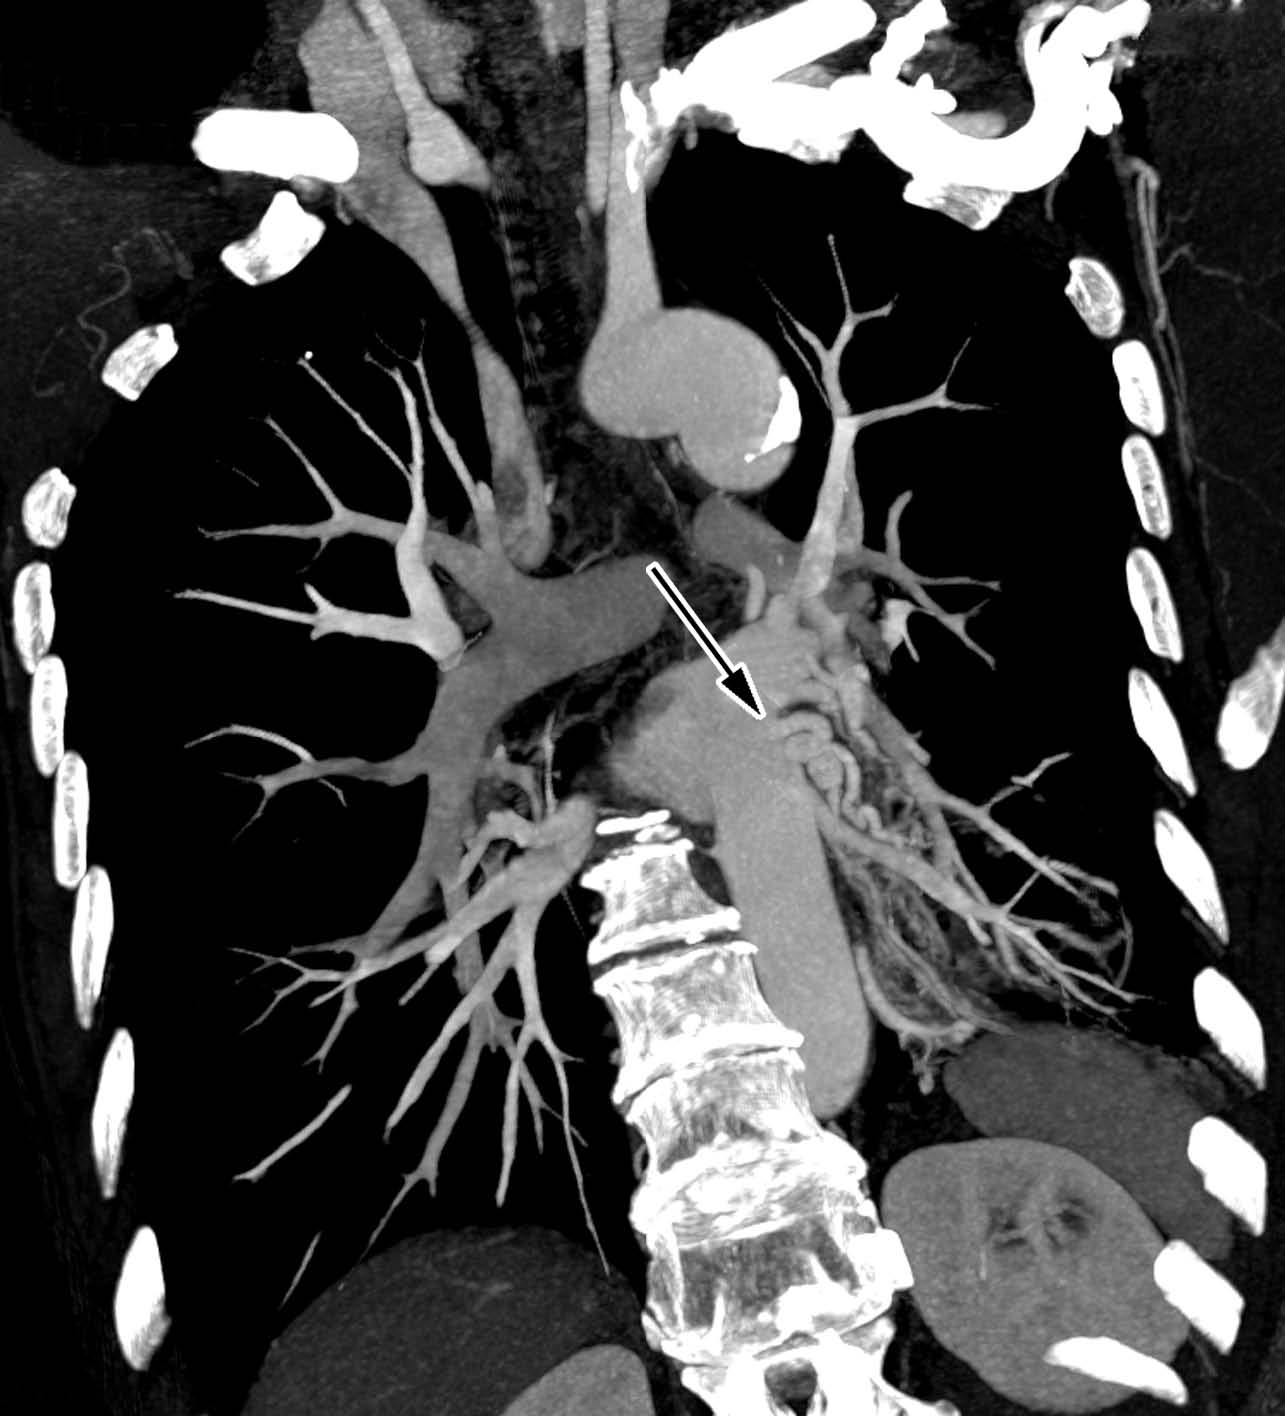
\includegraphics{./images/Image00145.jpg}
\end{minipage}}\\
\caption{}
\label{fig3-3-1}
\end{figure}

\textbf{【病史摘要】}  男性,69岁。咯血2天,以往体健。

\textbf{【X线表现】}
 X线正位胸片示左肺下叶脊柱旁见分叶状软组织影,边界光整,部分与心影重叠,内见半圆形气液面。同一患者胸部主动脉CT血管造影见病灶由降主动脉分支血管供血。

\textbf{【X线诊断】}  左肺下叶占位,肺隔离症可能。

\textbf{【评  述】}
 肺段隔离症是少见的先天畸形,为发生于胚胎前肠异常胚芽的肺组织团块,系指体循环动脉分支供应一部分发育不全、无呼吸功能而与正常肺组织相隔离的肺组织。肺段隔离症可发生于脏层胸膜内(叶内型,约占75%)和具有独自的胸膜(叶外型,约占25%)。大多数肺段隔离症发生于下胸部,但有5%~10%的肺外型肺段隔离症发生于膈下。膈下肺段隔离症发生于胸腹膜腔封闭前,肺组织遗留在腹腔。本病的供血动脉来自体动脉的异常分支,多数分支于主动脉,显示病灶供血动脉对诊断具有决定作用。一般无临床症状,但如隔离的肺段与支气管相通而发生继发感染时,则有发热、咳嗽、咳痰、咯血等症状。

X线表现为楔形或椭圆形致密影,边缘光滑、清楚,密度均匀。多位于左下叶后段脊柱旁沟,少数为右下叶后段,上叶少见;当病变与支气管相通时,可表现为含有气液平的囊肿形态。反复感染后阴影边缘模糊,周围支气管扩张;血管造影(采用主动脉造影)可显示有异常血管从主动脉发出进入病灶,供血动脉可为一支或多支,可见引流静脉。当发现肺内病灶供血来源于体动脉时,可确立诊断。

应与肺炎、肿瘤等鉴别,对年轻患者,X线发现左下叶后段实性或囊性病灶,无明显临床症状或反复发生感染,应考虑本病的存在。当X线胸片发现两下肺中线旁囊实性病灶时应怀疑本病的可能,进一步CT检查对诊断本病有极大帮助。高度怀疑本病时,应及时行胸部CTA或MRA检查,如能显示病变的供应血管来自胸或腹主动脉的异常分支,并能清楚显示这些分支起源的部位、数目和大小,则可确立诊断。肺叶内型回流到肺静脉,肺叶外型回流到体静脉系统,这是两型在X线上的唯一可靠区别。

\subsection{肺动静脉瘘}

\begin{figure}
  \centering
\subfloat[X线正位胸片]{
\begin{minipage}[b]{0.7\textwidth}
\centering
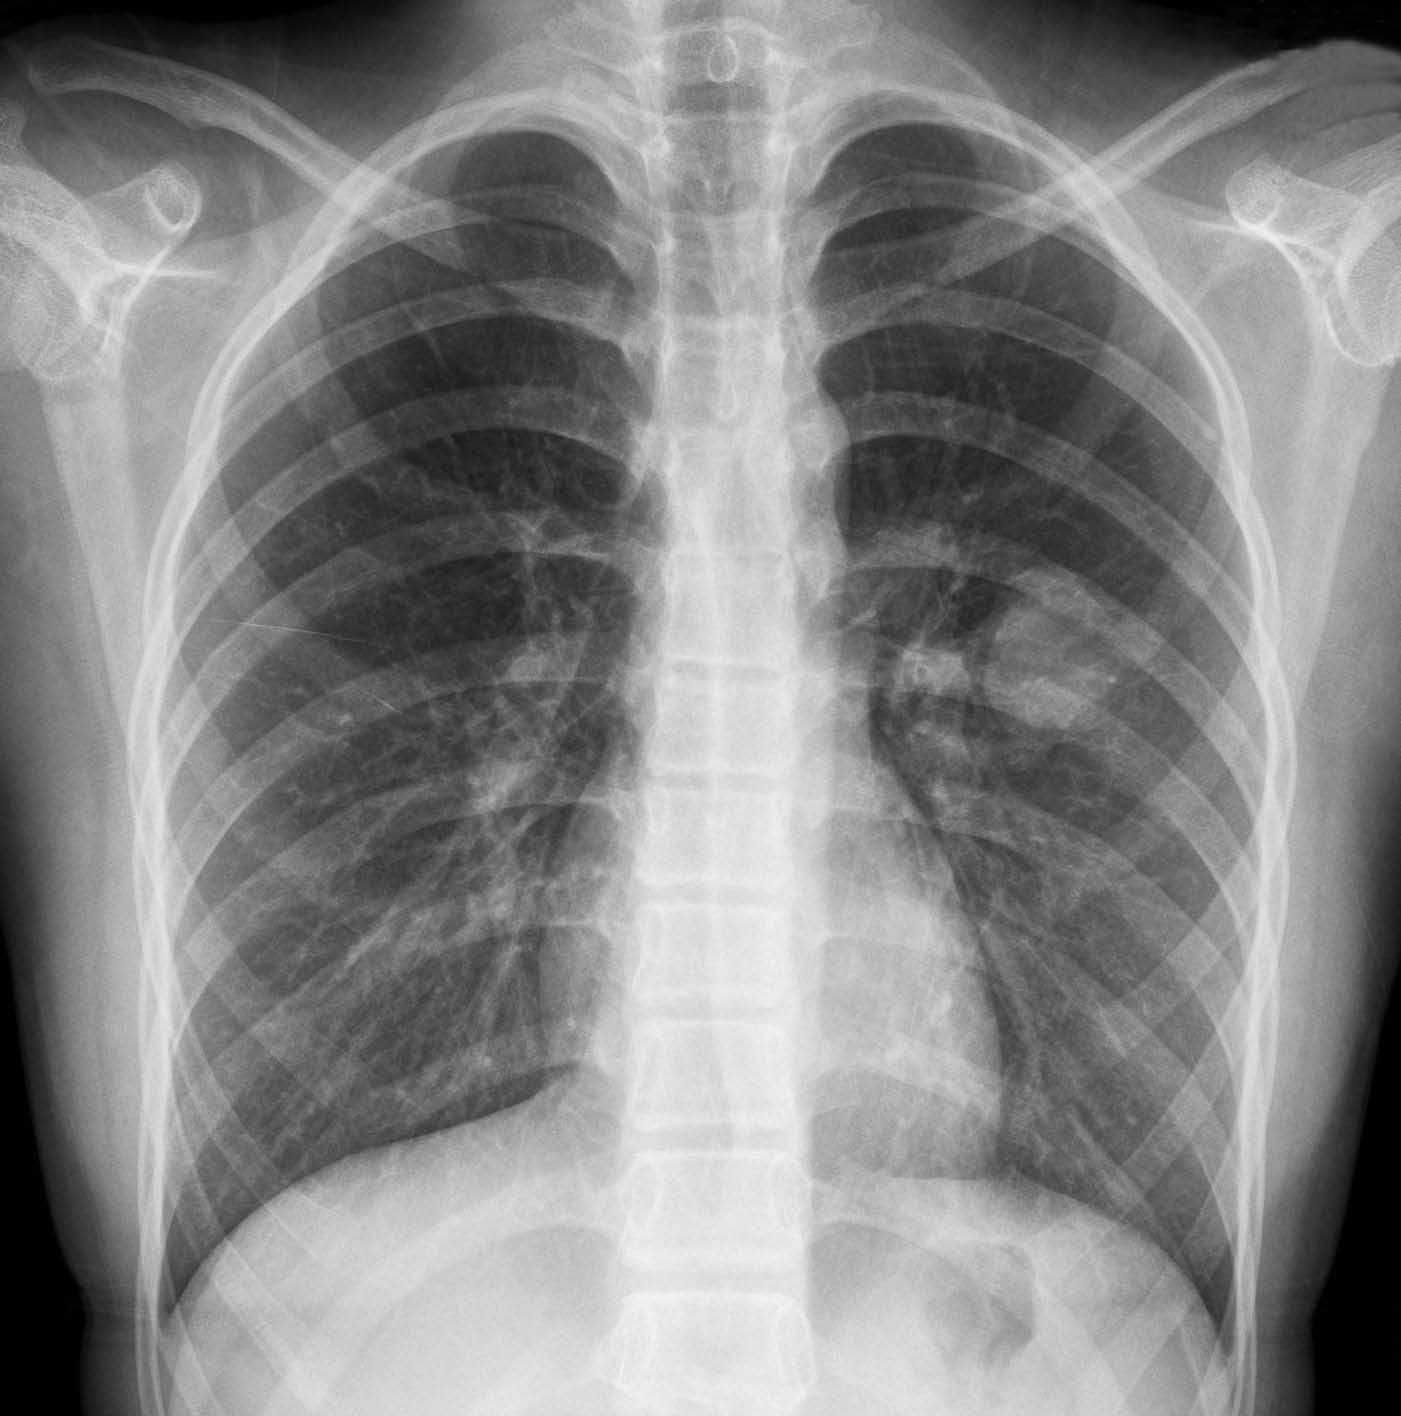
\includegraphics{./images/Image00146.jpg}
\end{minipage}}\\
\subfloat[胸部CT血管造影容积再现成像]{
\begin{minipage}[b]{0.7\textwidth}
\centering
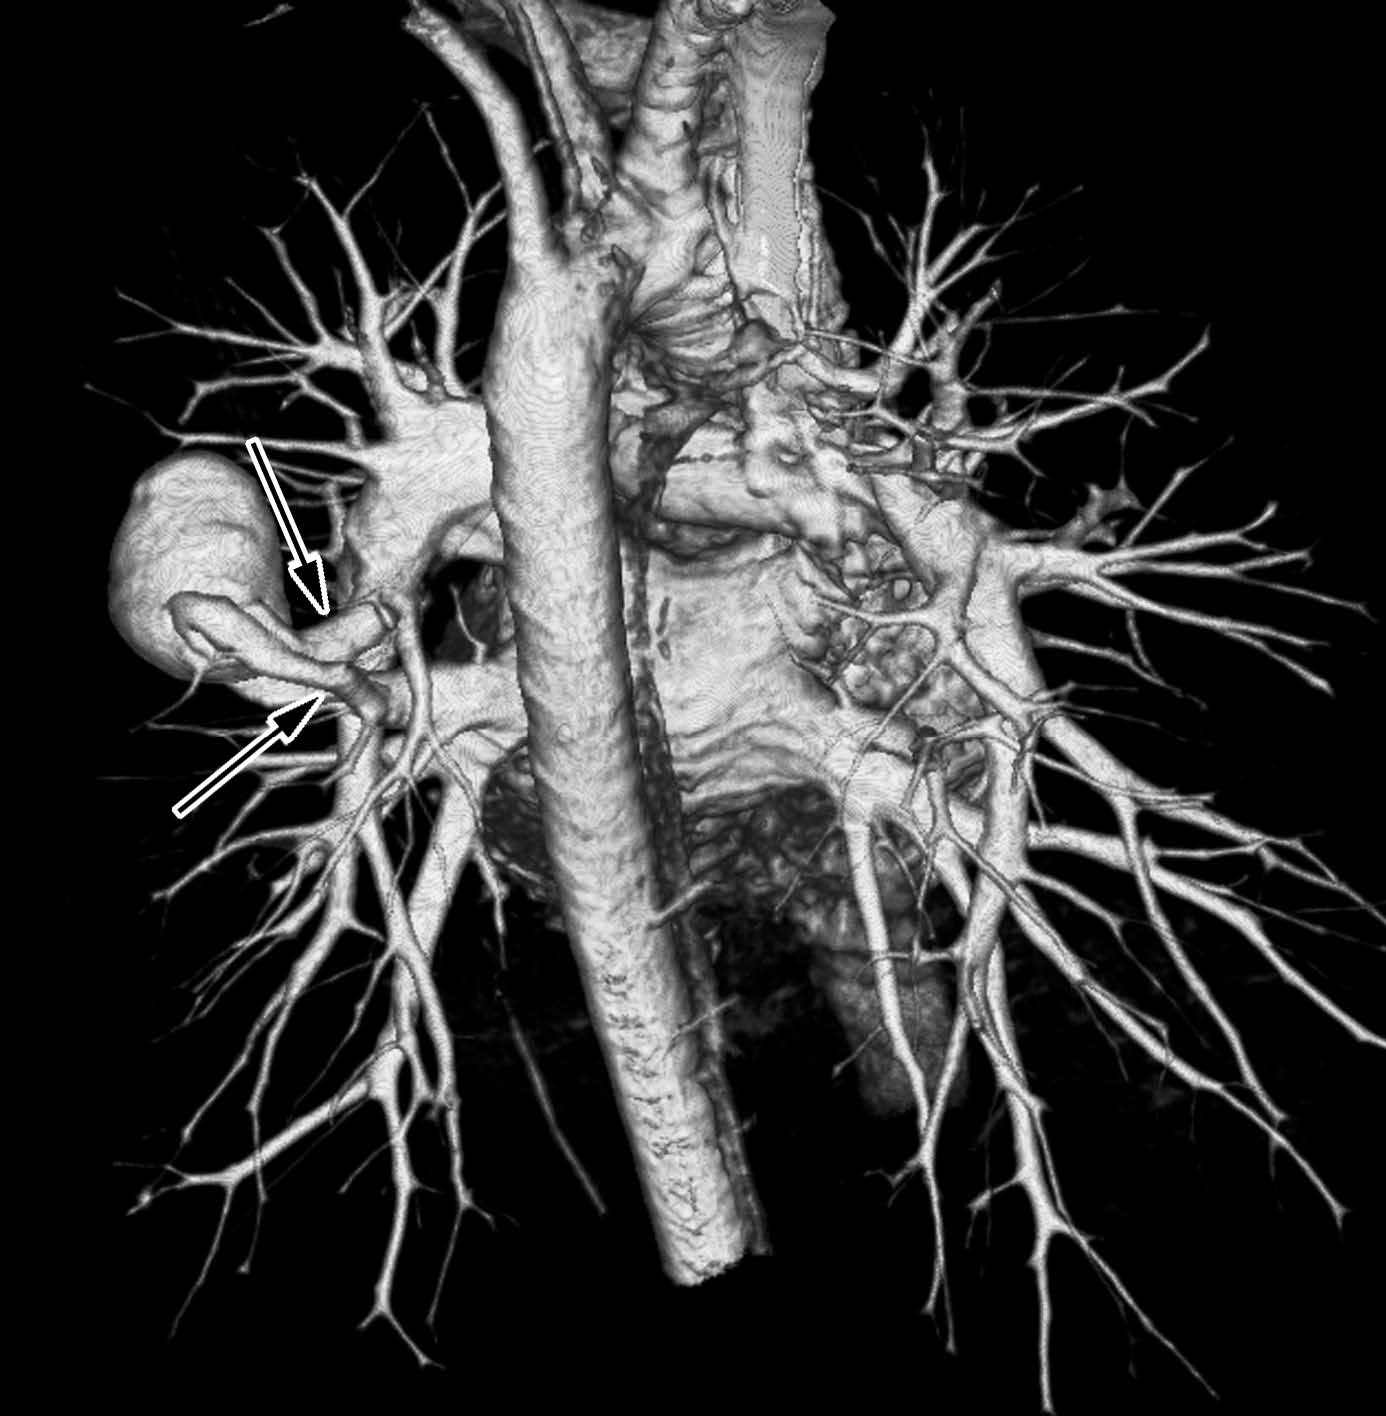
\includegraphics{./images/Image00147.jpg}
\end{minipage}}\\
\caption{}
\label{fig3-3-2}
\end{figure}

\textbf{【病史摘要】}  女性,12岁。体检发现左中肺野占位1天。

\textbf{【X线表现】}
 X线胸片示左中肺野软组织密度肿块影,边缘光整,呈土豆块状,近肺门侧见柔软条状影从左肺门走行入病灶内,纵隔、横膈影正常。同一患者胸部CT血管造影示左肺病灶呈血管瘤样强化,并见来自于左肺动脉的引入动脉和归属于左下肺静脉的引流静脉(箭头)。

\textbf{【X线诊断】}
 左肺中野良性占位,考虑肺动静脉瘘可能,建议进一步检查。

\textbf{【评  述】}
 肺动静脉瘘为先天性肺血管畸形,少数为肺创伤所致。血管扩大迂曲或形成海绵状血管瘤,肺动脉血液不经过肺泡直接流入肺静脉,肺动脉与静脉直接相通形成短路。病变血管壁肌层发育不良,缺乏弹力纤维,又因肺动脉压力促使病变血管进行性扩张,常形成肺动、静脉瘤,表现为局部血管扭曲、扩张及血管瘤形成。

本病多见于青年,分流量小者可无症状,仅在肺部X线检查时发现。分流量大者可出现活动后呼吸急促、发绀、杵状指(趾)、红细胞增多、皮肤粘膜可有出血点、斑或紫癜,局部可听到收缩期或双期杂音,但多在儿童期出现,偶见于新生儿。咯血是由于毛细血管扩张性病变位于支气管粘膜的病损或肺动静脉瘘的破裂而引起。

X线平片心影大小正常,但分流量大的肺动静脉瘘则有心脏扩大。约50%病例在胸片上显示单个或多个肿块状、球状、结节状、斑点状阴影,边缘光滑锐利,钙化少见,但常凹凸不平或呈分叶状,大小不一,位于1个或多个肺野。常可见一支或数支粗大扭曲的血管阴影,从肿块引向肺门,此点最具有诊断价值。肋骨侵蚀可因肋间动脉扩大所致,但不常见。透视时可见肿块有搏动,以停止呼吸时最清楚,有时可见肿块密度随搏动而改变,如患者做Valsalva动作,引起胸内压增高时,则见动静脉瘤缩小。

当X线平片不能明确诊断,需做鉴别诊断时,CT增强检查或CT血管造影(CTA)检查有助于该病的诊断。本例患者进一步做了胸部CTA检查,见左肺病灶呈血管样强化,并见来自于左肺动脉的引入动脉和归属于左下肺静脉的引流静脉(箭头),明确了诊断。

\section{肺部炎症}

\subsection{大叶性肺炎}

\begin{figure}
  \centering
\subfloat[正位X线胸片]{
\begin{minipage}[b]{0.7\textwidth}
\centering
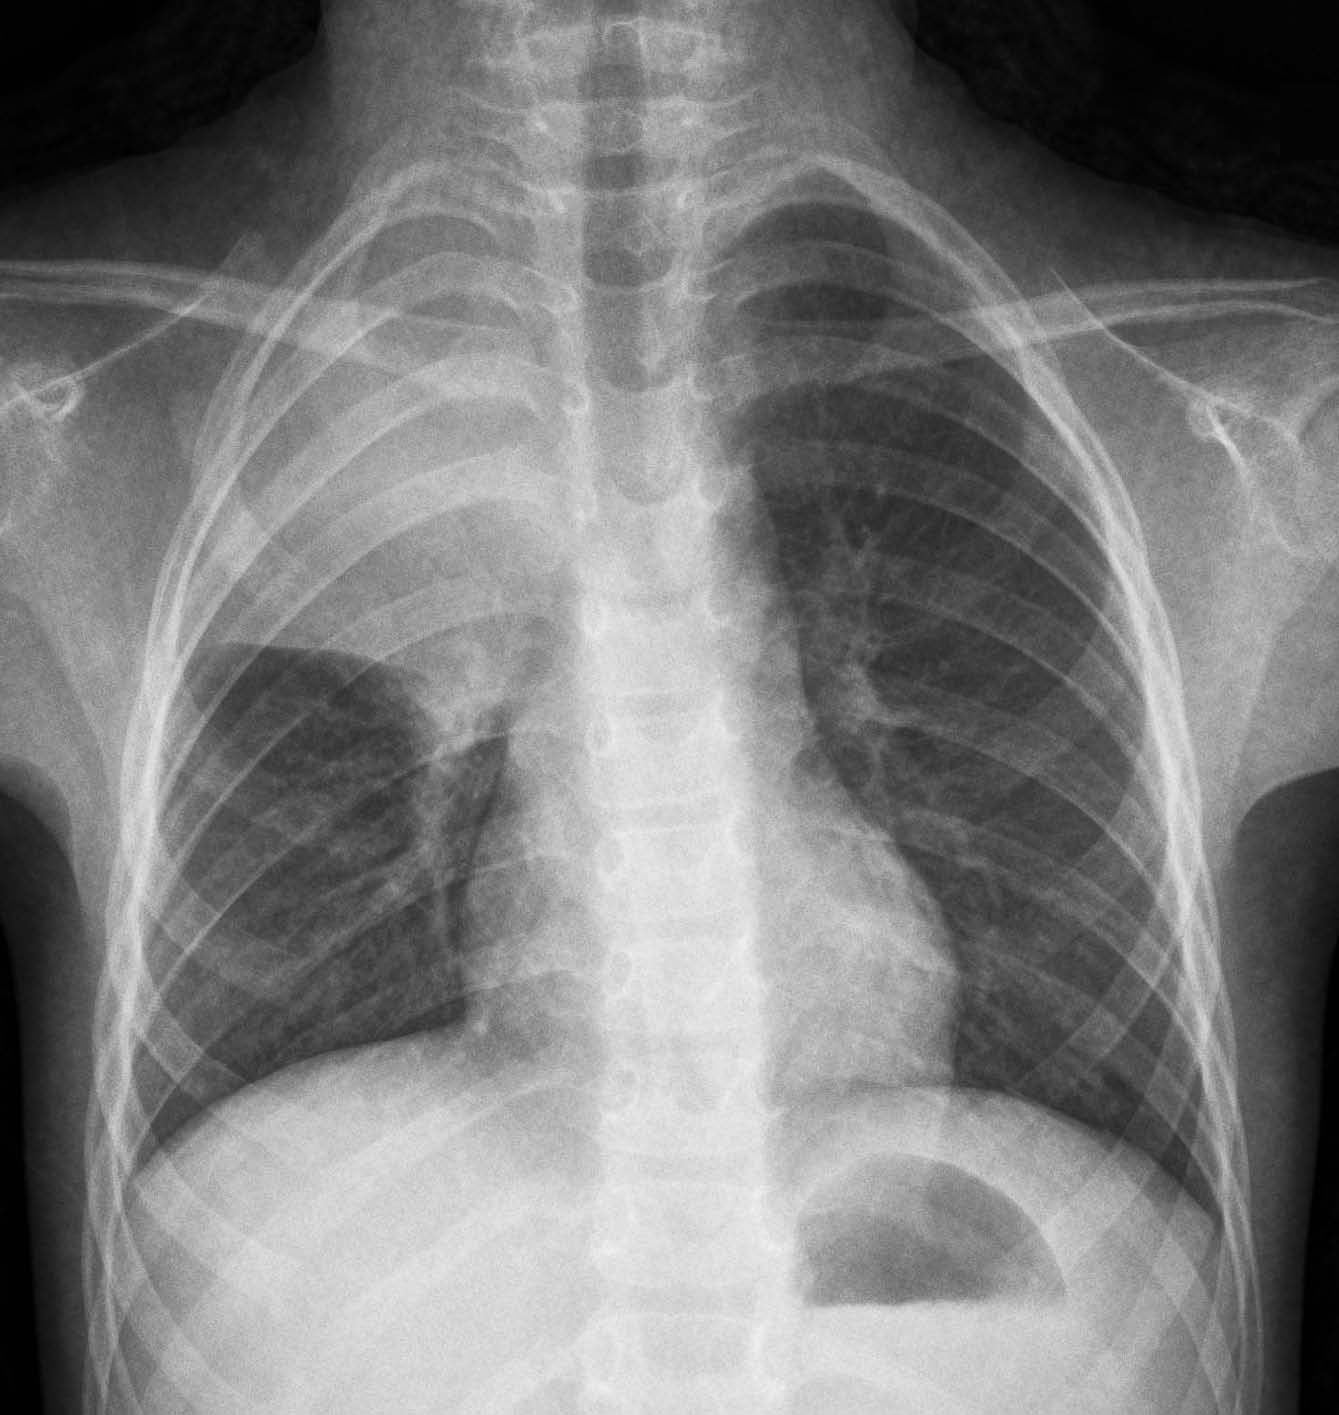
\includegraphics{./images/Image00148.jpg}
\end{minipage}}\\
\subfloat[右侧位X线胸片]{
\begin{minipage}[b]{0.7\textwidth}
\centering
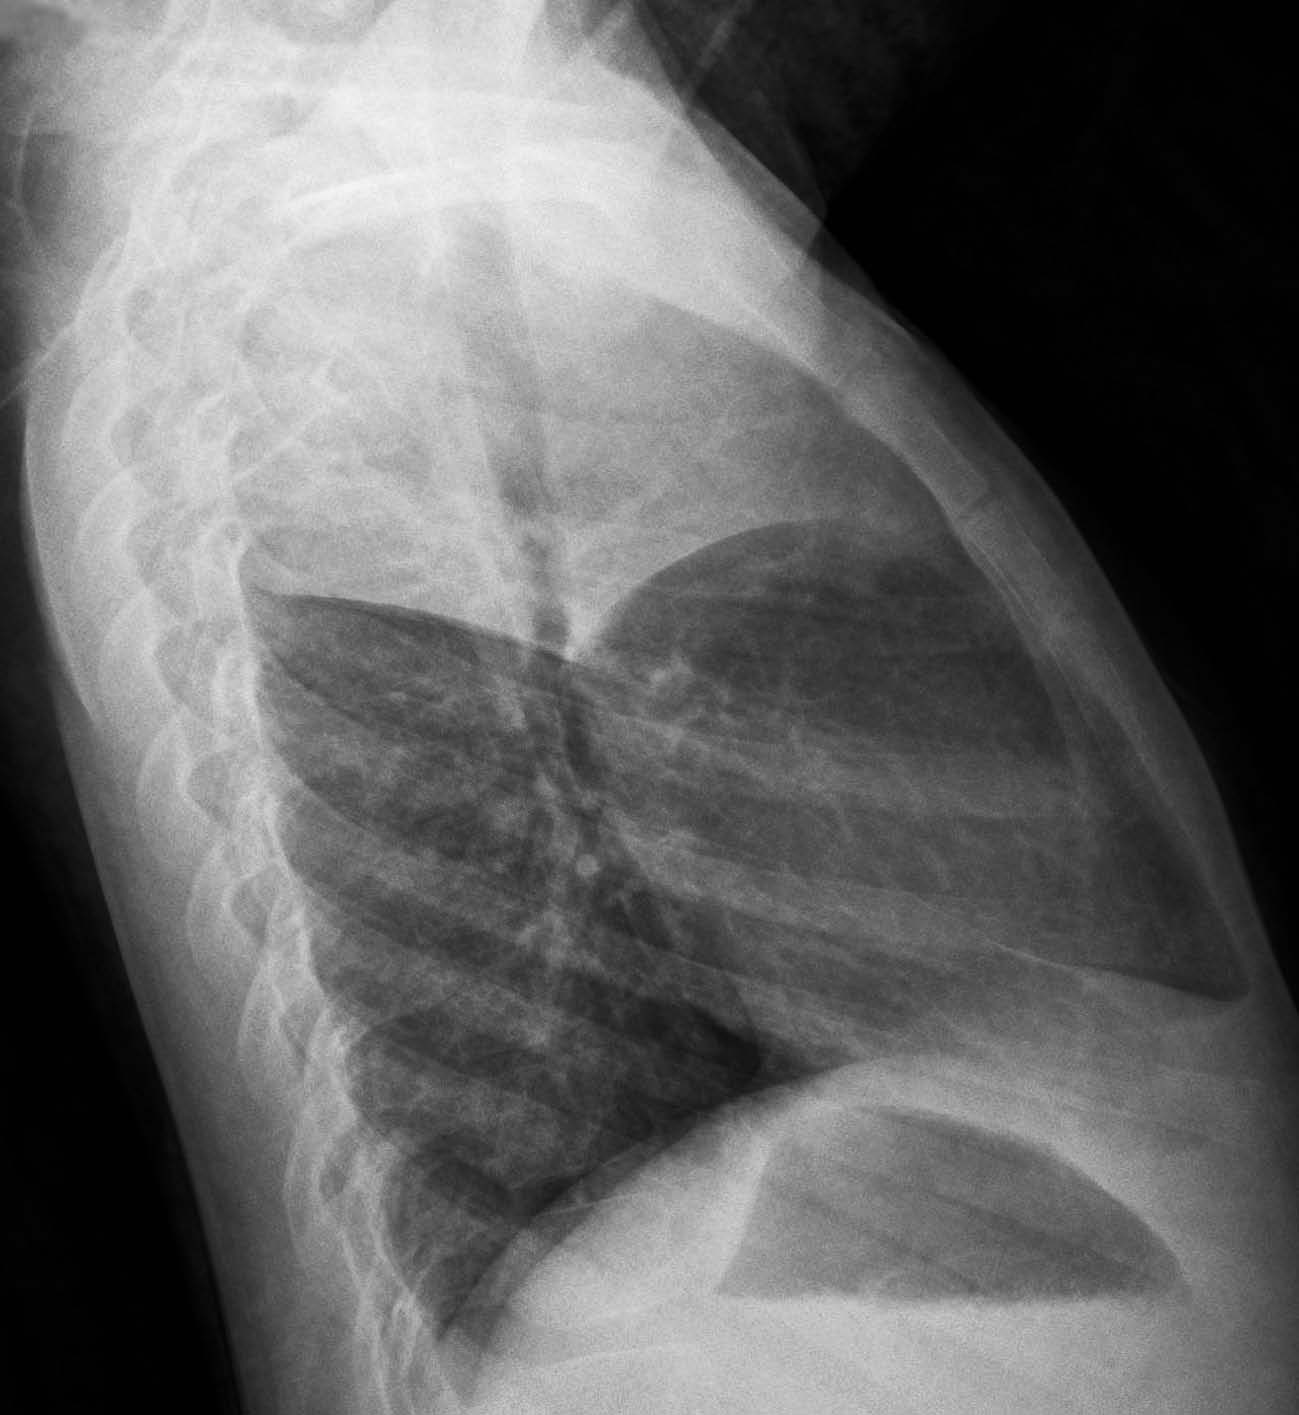
\includegraphics{./images/Image00149.jpg}
\end{minipage}}\\
\caption{}
\label{fig3-4-1}
\end{figure}

\textbf{【病史摘要】}
 男性,11岁。咳嗽、咳粘痰3天,寒战、发热1天。体格检查:面色潮红,呼吸急促,咽红,体温40.3℃;右上肺可闻及管状呼吸音。实验检查:白细胞计数13×10\textsuperscript{9}
/L,中性粒细胞比例增高。

\textbf{【X线表现】}
 X线正侧位胸片示右肺上叶呈大片致密实变影,右上肺体积未见明显缩小,心脏纵隔、气管未见移位,二膈位置正常。

\textbf{【X线诊断】}  右肺上叶大叶性肺炎。

\textbf{【评  述】}
 大叶性肺炎系肺炎链球菌或肺炎双球菌引起的急性实质性肺炎,由于有时病变呈大叶分布,习惯上称之为大叶性肺炎。由于本病扩散的特点是带细菌的渗出液通过肺泡孔从肺泡到肺泡,腺泡到腺泡,故实际上相当多的病例并不呈大叶或肺段分布。

典型的病理变化分为四期,即充血期、红色肝样变期、灰色肝样变期及消散期。早期为充血期,病变部位毛细血管充血扩张,肺泡内仍有空气但可有少量浆液性渗出。此后肺泡内充满粘稠的渗出液,其中有纤维素和许多红细胞,使肺组织切面呈红色,为红色肝样变期。随病变发展,肺泡内红细胞减少,代之以大量白细胞,肺组织切面呈灰色,为灰色肝样变期。经及时治疗,1周后开始转入消散期,肺泡内纤维蛋白渗出物溶解、吸收,肺泡重新充气。多数患者发病前有受凉、过度劳累或上呼吸道感染。起病急,寒战、高热、胸痛、咳较粘稠或为典型铁锈色痰。下叶肺炎可刺激膈胸膜,疼痛放射至腹部。血白细胞计数及中性粒细胞明显增高。

大叶性肺炎充血期的X线表现有时可无阳性发现,或仅肺纹理增多,透明度略低。至实变期(包括红色肝样变期及灰色肝样变期)表现为密度均匀的致密影,炎症累及肺段表现为片状或三角形致密影;累及整个肺叶,呈以叶间裂为界的大片致密阴影,有时致密阴影内,可见透亮支气管影,即支气管充气征。消散期时实变区密度逐渐减低,由于病变的消散不均,表现为大小不等、分布不规则的斑片状阴影。炎症最终可完全吸收,或只留少量索条状阴影,偶可机化演变为机化性肺炎。

急性大叶性肺炎有典型临床表现,结合胸部X线片即可确诊。当X线表现不典型时应与阻塞性肺炎、大叶性干酪肺炎等相鉴别。阻塞性肺炎肺叶体积明显缩小,邻近组织结构向病变区移位。大叶性干酪肺炎的患者情况一般较衰竭,痰结核菌阳性,实变区密度不均匀,常可见蜂窝样空洞,病变肺叶体积一般有缩小,其他肺野有播散病灶,短期复查病变不吸收。

\subsection{支气管肺炎}

\begin{figure}[!htbp]
 \centering
 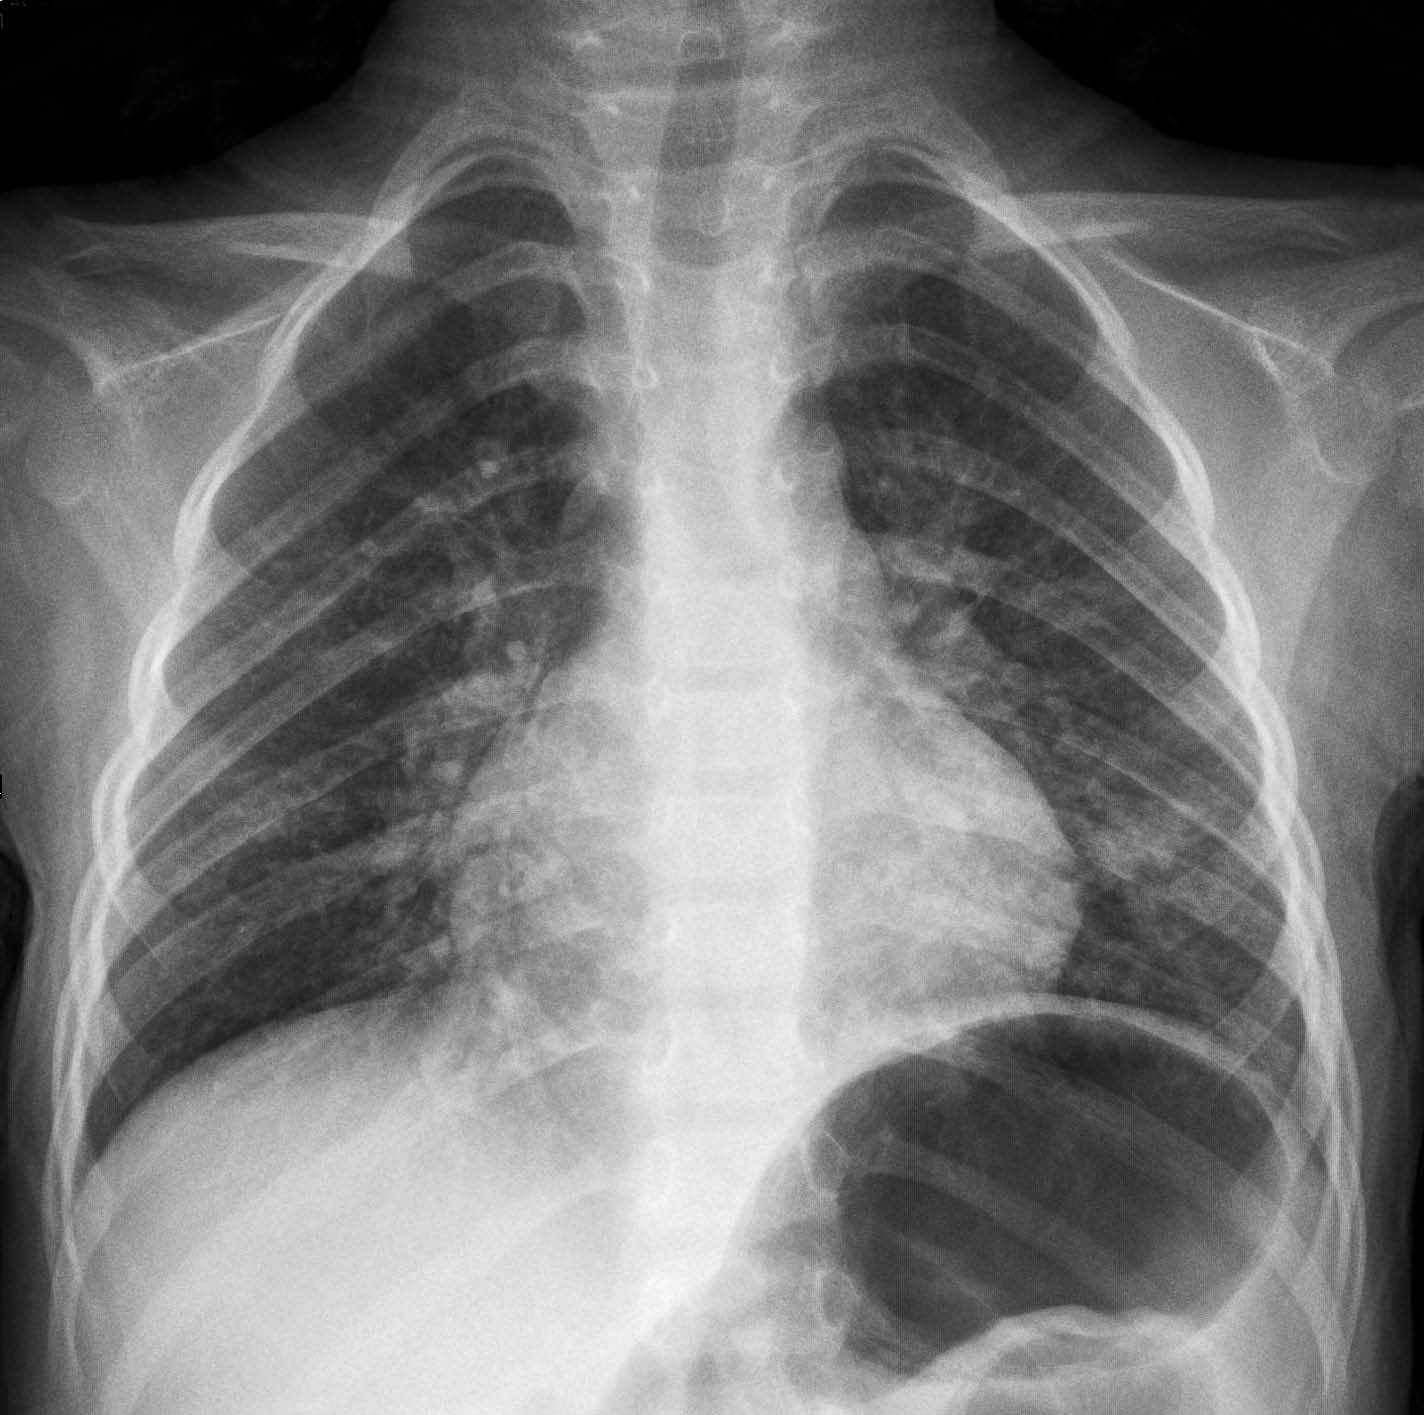
\includegraphics{./images/Image00150.jpg}
 \captionsetup{justification=centering}
 \caption{正位X线胸片示支气管肺炎}
 \label{fig3-4-2}
  \end{figure} 

\textbf{【病史摘要】}
 女性,7岁。咳嗽、咳少量粘痰1周,发热2天,体温38.7℃。体格检查:两肺可闻及湿啰音。

\textbf{【X线表现】}
 两肺纹理增多,纹理边缘模糊不清,沿肺纹理见散在斑点、斑片状模糊影。胃腔积气致左膈升高。

\textbf{【X线诊断】}  两肺支气管肺炎。

\textbf{【评  述】}
 支气管肺炎,亦称小叶性肺炎;多见于婴幼儿、青少年和老年及极度衰弱的患者,或为手术后并发症。可由细菌或病毒引起,按病理形态的改变分为一般支气管肺炎和间质性支气管肺炎两类,前者多由细菌所致,后者则以病毒为主,临床常笼统地诊断为支气管肺炎。病理变化为支气管周围的肺实质炎症,以小叶支气管为中心经过终末细支气管累及肺泡,在支气管和肺泡内产生炎性渗出物。病变范围是小叶性的,呈散在性两侧分布,但可融合成大片。由于细支气管炎性充血、水肿,易致细支气管不同程度的阻塞,可出现小叶性肺气肿或肺不张。

支气管肺炎多发生于冬春季节及气候骤变时,临床表现发病急骤,有高热寒战、咳嗽、咳泡沫粘液脓性痰,常有胸痛,呼吸困难。因支气管肺炎多为其他疾病的并发症,其临床症状常被原发疾病所掩盖,但发热、咳嗽和咳痰仍是最常见的症状。支气管粘膜受炎症及渗出物的刺激引起咳嗽,痰液往往为粘液脓性或脓性。因病变常呈小灶性分布,故肺实变体征不明显,由于病变部位细支气管和肺泡腔内含有渗出物,听诊可闻及湿啰音。

X线表现为肺纹理增多、增粗、模糊。沿肺纹理分布有小斑片状肺实质浸润阴影,密度不均,以两肺下野、心膈角区及中内带较多。小斑片病灶可部分融合在一起成为大片状浸润影,甚至可类似节段或大叶肺炎的形态。若病变中出现较多的小圆形病灶时,就应考虑可能有化脓性感染存在。有时可出现肺间质性肺炎X线征象,常见两肺中内带纹理增多、模糊或出现条状阴影,甚至聚集而成网状;这些间质的改变与两肺下野的肺过度充气而呈现明亮的肺气肿区域形成鲜明的对比;流感病毒性肺炎、麻疹病毒性肺炎、百日咳杆菌肺炎所引起的肺间质炎性的反应都可有这些X线征象。

支气管肺炎有明显的临床症状,典型病例通常X线胸片即可诊断,一般不需CT检查。对迁延或反复发作者,CT检查旨在了解有无并发支气管扩张或与其他疾病相鉴别。

\subsection{肺炎性假瘤}

\begin{figure}[!htbp]
 \centering
 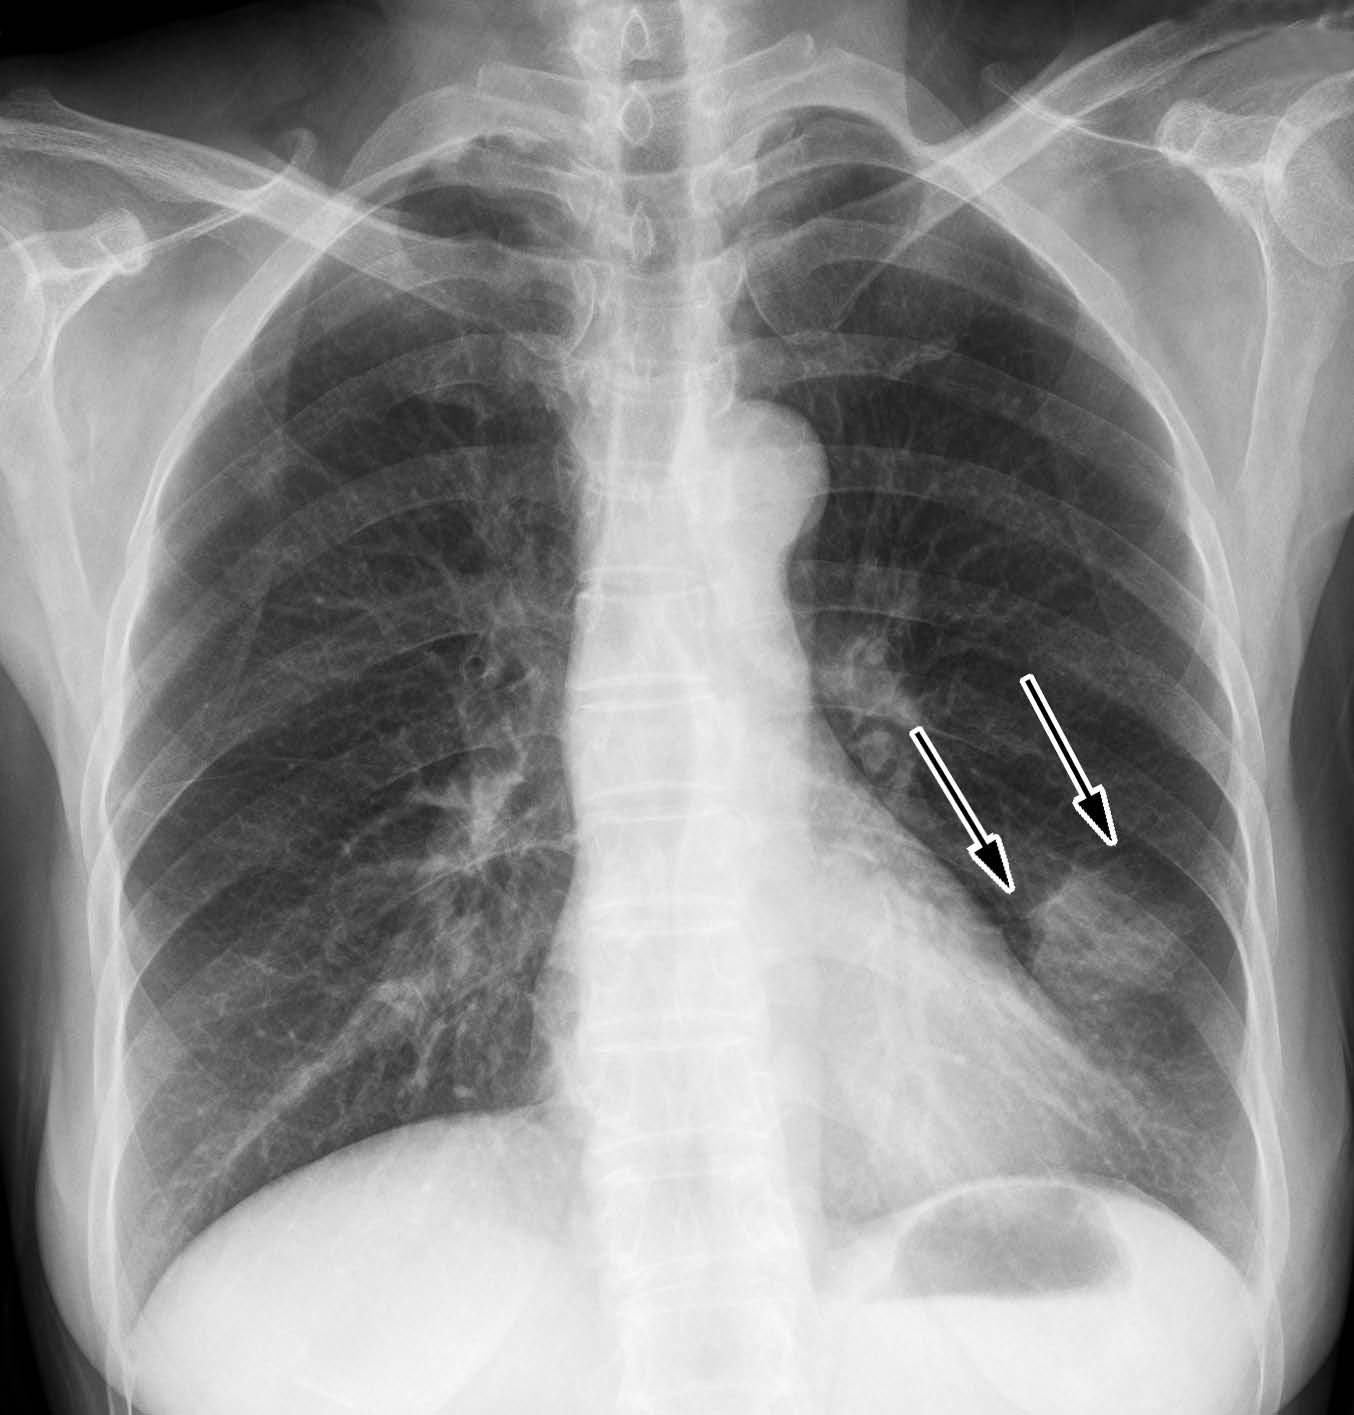
\includegraphics{./images/Image00151.jpg}
 \captionsetup{justification=centering}
 \caption{正位X线胸片示左下肺占位}
 \label{fig3-4-3}
  \end{figure} 

\textbf{【病史摘要】}
 女性,67岁。咳嗽伴左下胸痛10天,有时有血痰。体格检查:两肺呼吸音粗。

\textbf{【X线表现】}
 左下肺见略呈分叶状软组织肿块影,边缘清晰,病灶上缘见尖角样影(箭头)。

\textbf{【X线诊断】}
 左肺下叶占位,肺炎性假瘤可能,周围型肺癌待排除,建议进一步检查。

\textbf{【评  述】}
 肺炎性假瘤是肺内良性肿块,是由肺内慢性炎症产生的肉芽肿、机化、纤维结缔组织增生及相关的继发病变形成的肿块,并非真正肿瘤。病理学特征是组织学的多形性,主要为成纤维细胞、各种炎症细胞、组织细胞及血管等多种成分组成的肉芽肿,根据组织成分的不同可分为组织细胞瘤型、硬化性血管瘤型、浆细胞肉芽肿型、假性淋巴瘤型的肺泡上皮增生型。病原及发病机制尚不清楚。

肺炎性假瘤一般位于肺实质内,其大体形态为肺实质内的球形肿块,压迫周围肺组织形成假包膜,累及支气管的仅占少数。绝大多数单发,呈圆形或椭圆形结节,一般无完整的包膜,但肿块较局限、边界清楚,有些还有较厚而缺少细胞的胶原纤维结缔组织与肺实质分开。少数肺炎性假瘤可以发生癌变。

肺炎性假瘤患者多数年龄在50岁以下,女性略多于男性。约1/3的患者没有临床症状,仅偶然在X线检查时发现,2/3的患者有慢性支气管炎、肺炎、肺化脓症的病史,以及相应的临床症状,如咳嗽、咳痰、低热,部分患者还有胸痛、血痰,甚至咯血,但咯血量一般较少。

肺炎性假瘤X线表现可发生在两肺的任何部位,但多位于下叶背段和内后基底段。球形瘤体由于有较完整的假性包膜,因此轮廓清楚,边缘光滑,周围肺野清晰,直径多在1~4cm,密度比较均匀。团块状的瘤体由于假包膜不完整,一般边界不清,边缘模糊,部分病灶密度浓淡不匀,如多次并发急性炎症可造成病灶阴影扩大,在其周围恰似炎性浸润的片状影。因此,肺炎性假瘤边缘清楚与否取决于肿块周围的病理变化,边界面清楚者,瘤体周围一般有假性包膜;若病灶处于急性阶段时,假瘤周围显示炎性,渗出在瘤体周围多呈模糊影亦无假包膜形成。少数可出现空洞、囊性化或钙化。有学者认为病灶周围出现桃尖征、尖角征、长毛刺、与胸膜紧贴或有粘连带等X线征象对本病的诊断具有一定的意义,本例患者胸部X线显示病灶上缘见尖角征(箭头),经手术病理证实为肺炎性假瘤。

肺炎性假瘤在诊断上很难与肺癌、肺结核球、错构瘤等相鉴别,给临床治疗带来很大的困难。其中最重要的是与肺癌相鉴别,这直接关系到治疗的方法及手术切除的范围;从病史上看,炎性假瘤患者年龄一般较轻,多无长期吸烟史,全身情况多无明显变化,可有一过性发热史,无持续的痰中带血,无肺外症状;从影像学上看,炎性假瘤一般位于肺的周边,呈孤立肿块影,也可呈多发病灶,大小不等,肿块密度多均匀,可有钙化、空洞,但这种情况少见,大部分炎性假瘤周围可见斑点状或条带状影,炎性假瘤瘤体增长缓慢或长期无增长,在痰的检查、支气管镜活检中查不到癌细胞;而肺癌的肿块多呈分叶状,边缘毛糙不光滑,密度不均匀,坏死区密度更低,这可能与肿瘤组织生长较活跃有关,可伴胸腔积液,肺门及纵隔淋巴结转移较多;肺炎性假瘤可出现边缘不整、毛刺甚至分叶,而肺癌也可出现钙化、空洞等征象,常规影像检查难以将二者区别,有人主张通过抗炎动态观察,如病变缩小甚至消失,则可认为是肺炎性假瘤;但是,肺炎性假瘤的形成是一个较长的慢性过程,一旦形成,抗感染治疗极少能起作用,除非假瘤未完全形成。因此,当二者鉴别困难时,进一步的检查是必需的,胸部CT(平扫+增强)、经胸壁肿块穿刺活检或经纤维支气管镜活检对鉴别诊断是有帮助的。

结核球易发生在肺的上叶尖后段或下叶背段,密度均匀,可有钙化,病灶周围常有卫星灶;错构瘤为肺内边界光整、瘤内有典型爆米花样钙化。可与肺炎性假瘤区别。

\subsection{急性肺脓肿}

\begin{figure}[!htbp]
 \centering
 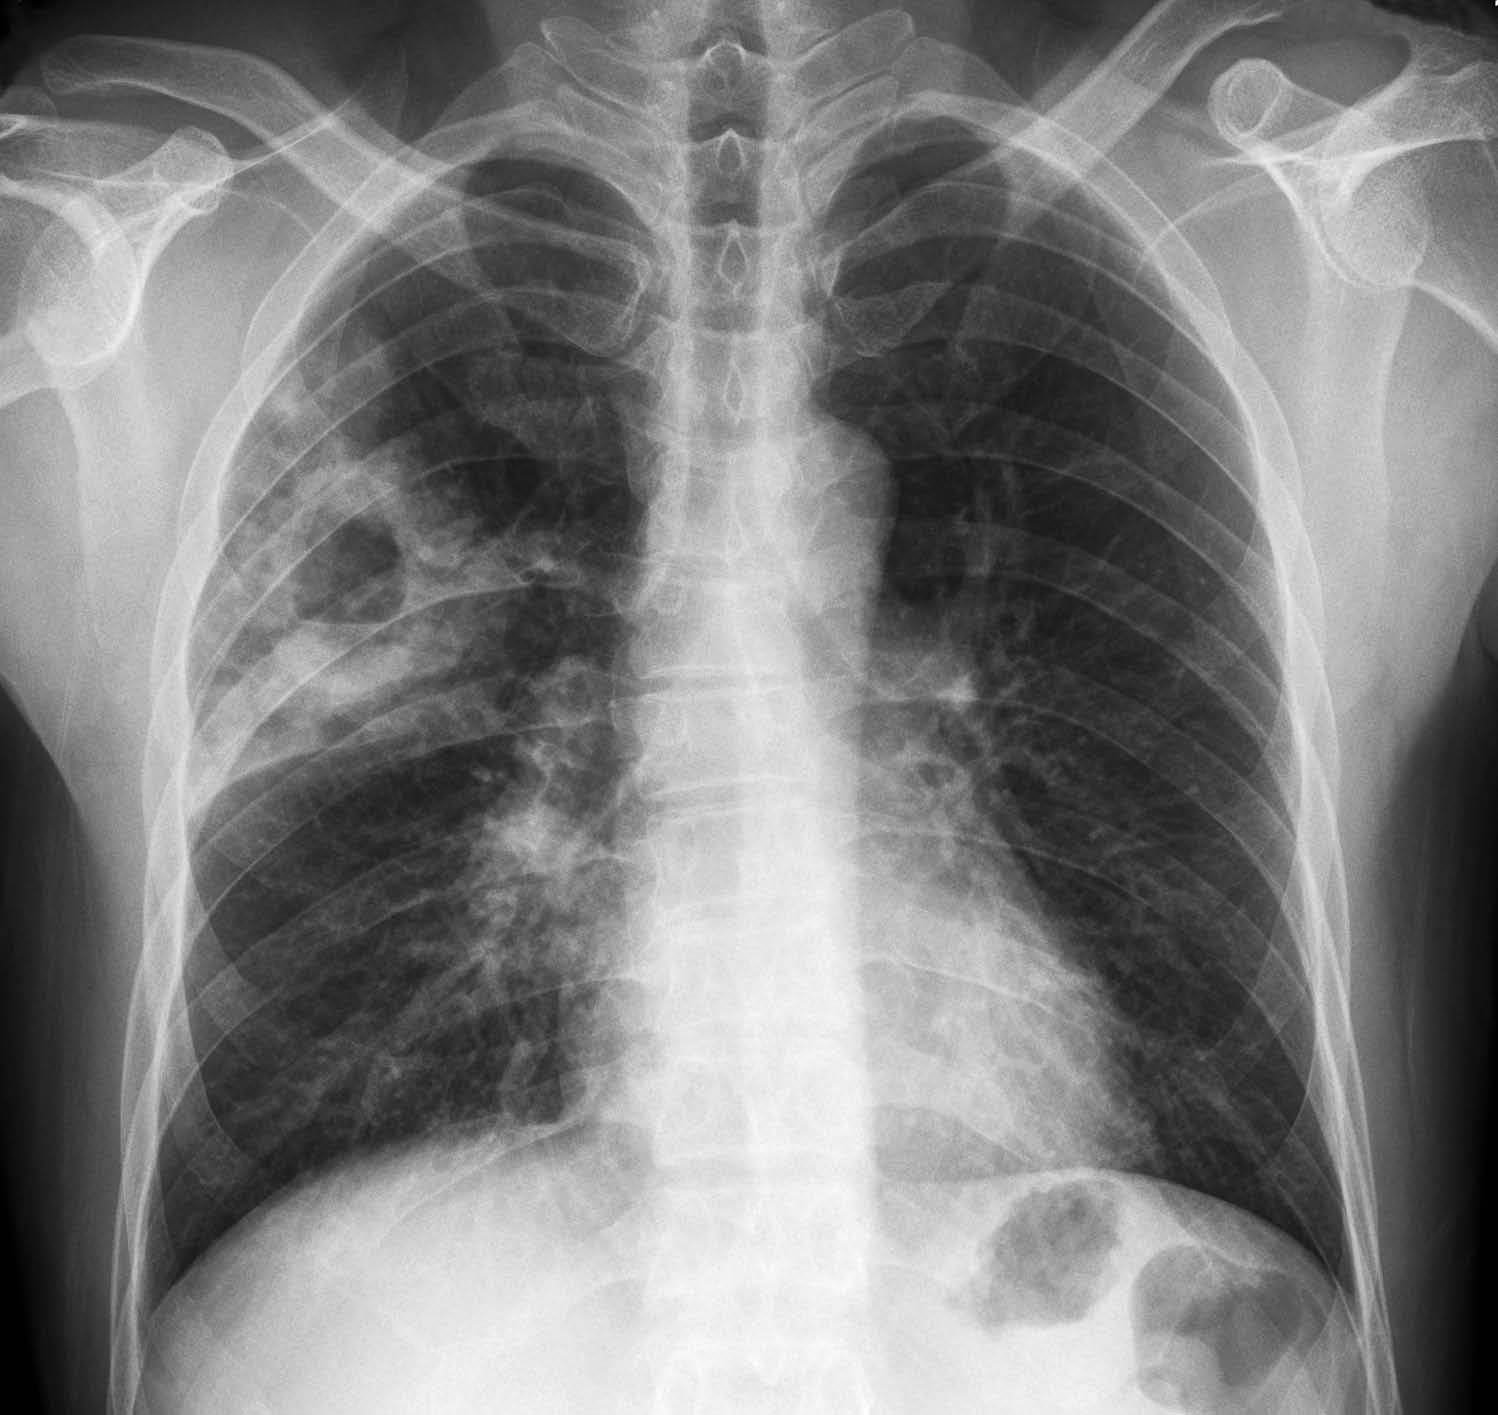
\includegraphics{./images/Image00152.jpg}
 \captionsetup{justification=centering}
 \caption{正位X线胸片示右上肺肺脓肿}
 \label{fig3-4-4}
  \end{figure} 

\textbf{【病史摘要】}
 男性,37岁。咳嗽、咳痰伴发热5天。体格检查:体温38.4℃,呼吸急促。肺部听诊右上肺呼吸音低,局部可闻及湿啰音,叩诊呈浊音。实验室检查:白细胞计数12.5×10\textsuperscript{9}
/L,中性粒细胞73%。

\textbf{【X线表现】}
 右上肺大片状边缘模糊影,下缘为水平裂所限而相对光整,水平裂位置正常;病灶内见厚壁空洞影,空洞内壁光整,内见气液面;心脏大小、左肺正常。

\textbf{【X线诊断】}  右上肺脓肿。

\textbf{【评  述】}
 急性肺脓肿主要是球菌和厌氧菌等引起的肺实质化脓性炎症、坏死和液化,常为一个肺段或亚肺段的急性炎症坏死,开始为实体性,但迅速液化并与支气管沟通,排出脓液形成X线可见的空洞。早期有高热、寒战、咳嗽、胸痛、白细胞计数增高等急性炎症症状,脓腔与支气管沟通后,咯出大量脓臭痰,随后体温下降,症状减轻。

X线早期表现为大片炎性实变阴影,边缘模糊,密度均匀增高,在加深曝光或体层片上有时可见一个或数个小的密度减低区;排脓以后,主要表现为一个厚壁空洞,空洞外缘有较广泛的炎性浸润而模糊不清,空洞内缘毛糙不整,呈虫蚀状;但也可光整,洞内常有宽大的液平面;病变常靠近肺边缘,相邻的胸膜增厚或伴有胸腔积液;有时病变可穿过叶间裂,蔓延到邻近肺叶;若引流不畅可形成张力空洞,洞形变圆,鼓胀,洞壁变薄;空洞周围及其他肺野一般没有播散病灶;一般看不到引流支气管,抗菌治疗后,空洞周围炎症可迅速吸收,空洞缩小以至消失,也可残留少量纤维病灶。

需与肺结核空洞、癌性空洞合并感染相鉴别,前者常无明显急性炎症症状;多数空洞壁较薄,内外缘较清楚;空洞内一般无液体,或仅有浅小的液平面;空洞周围多有小结节或斑点状卫星病灶,其他肺野可有播散病灶;空洞与肺门之间常可见轨道样引流支气管;短期治疗观察无变化,可与急性肺脓肿相鉴别。癌性空洞合并感染时,空洞内可有积液,空洞周围可有炎性浸润,临床有急性感染症状,故易误为肺脓肿;但常可见部分边缘比较清楚,并显示出分叶、毛刺等癌肿征象;空洞壁厚薄不均,洞内缘凹凸不平,有结节状凸出;有时可见支气管呈漏斗状或鼠尾样狭窄;肺门及纵隔有时可见肿大的淋巴结;短期抗感染治疗后,炎症消退可显示出癌性空洞原貌。X线影像结合临床病史、相关实验室检查常可确立诊断,进一步CT检查可提供更多的影像信息。

\section{肺结核}

\subsection{原发性肺结核}

\begin{figure}[!htbp]
 \centering
 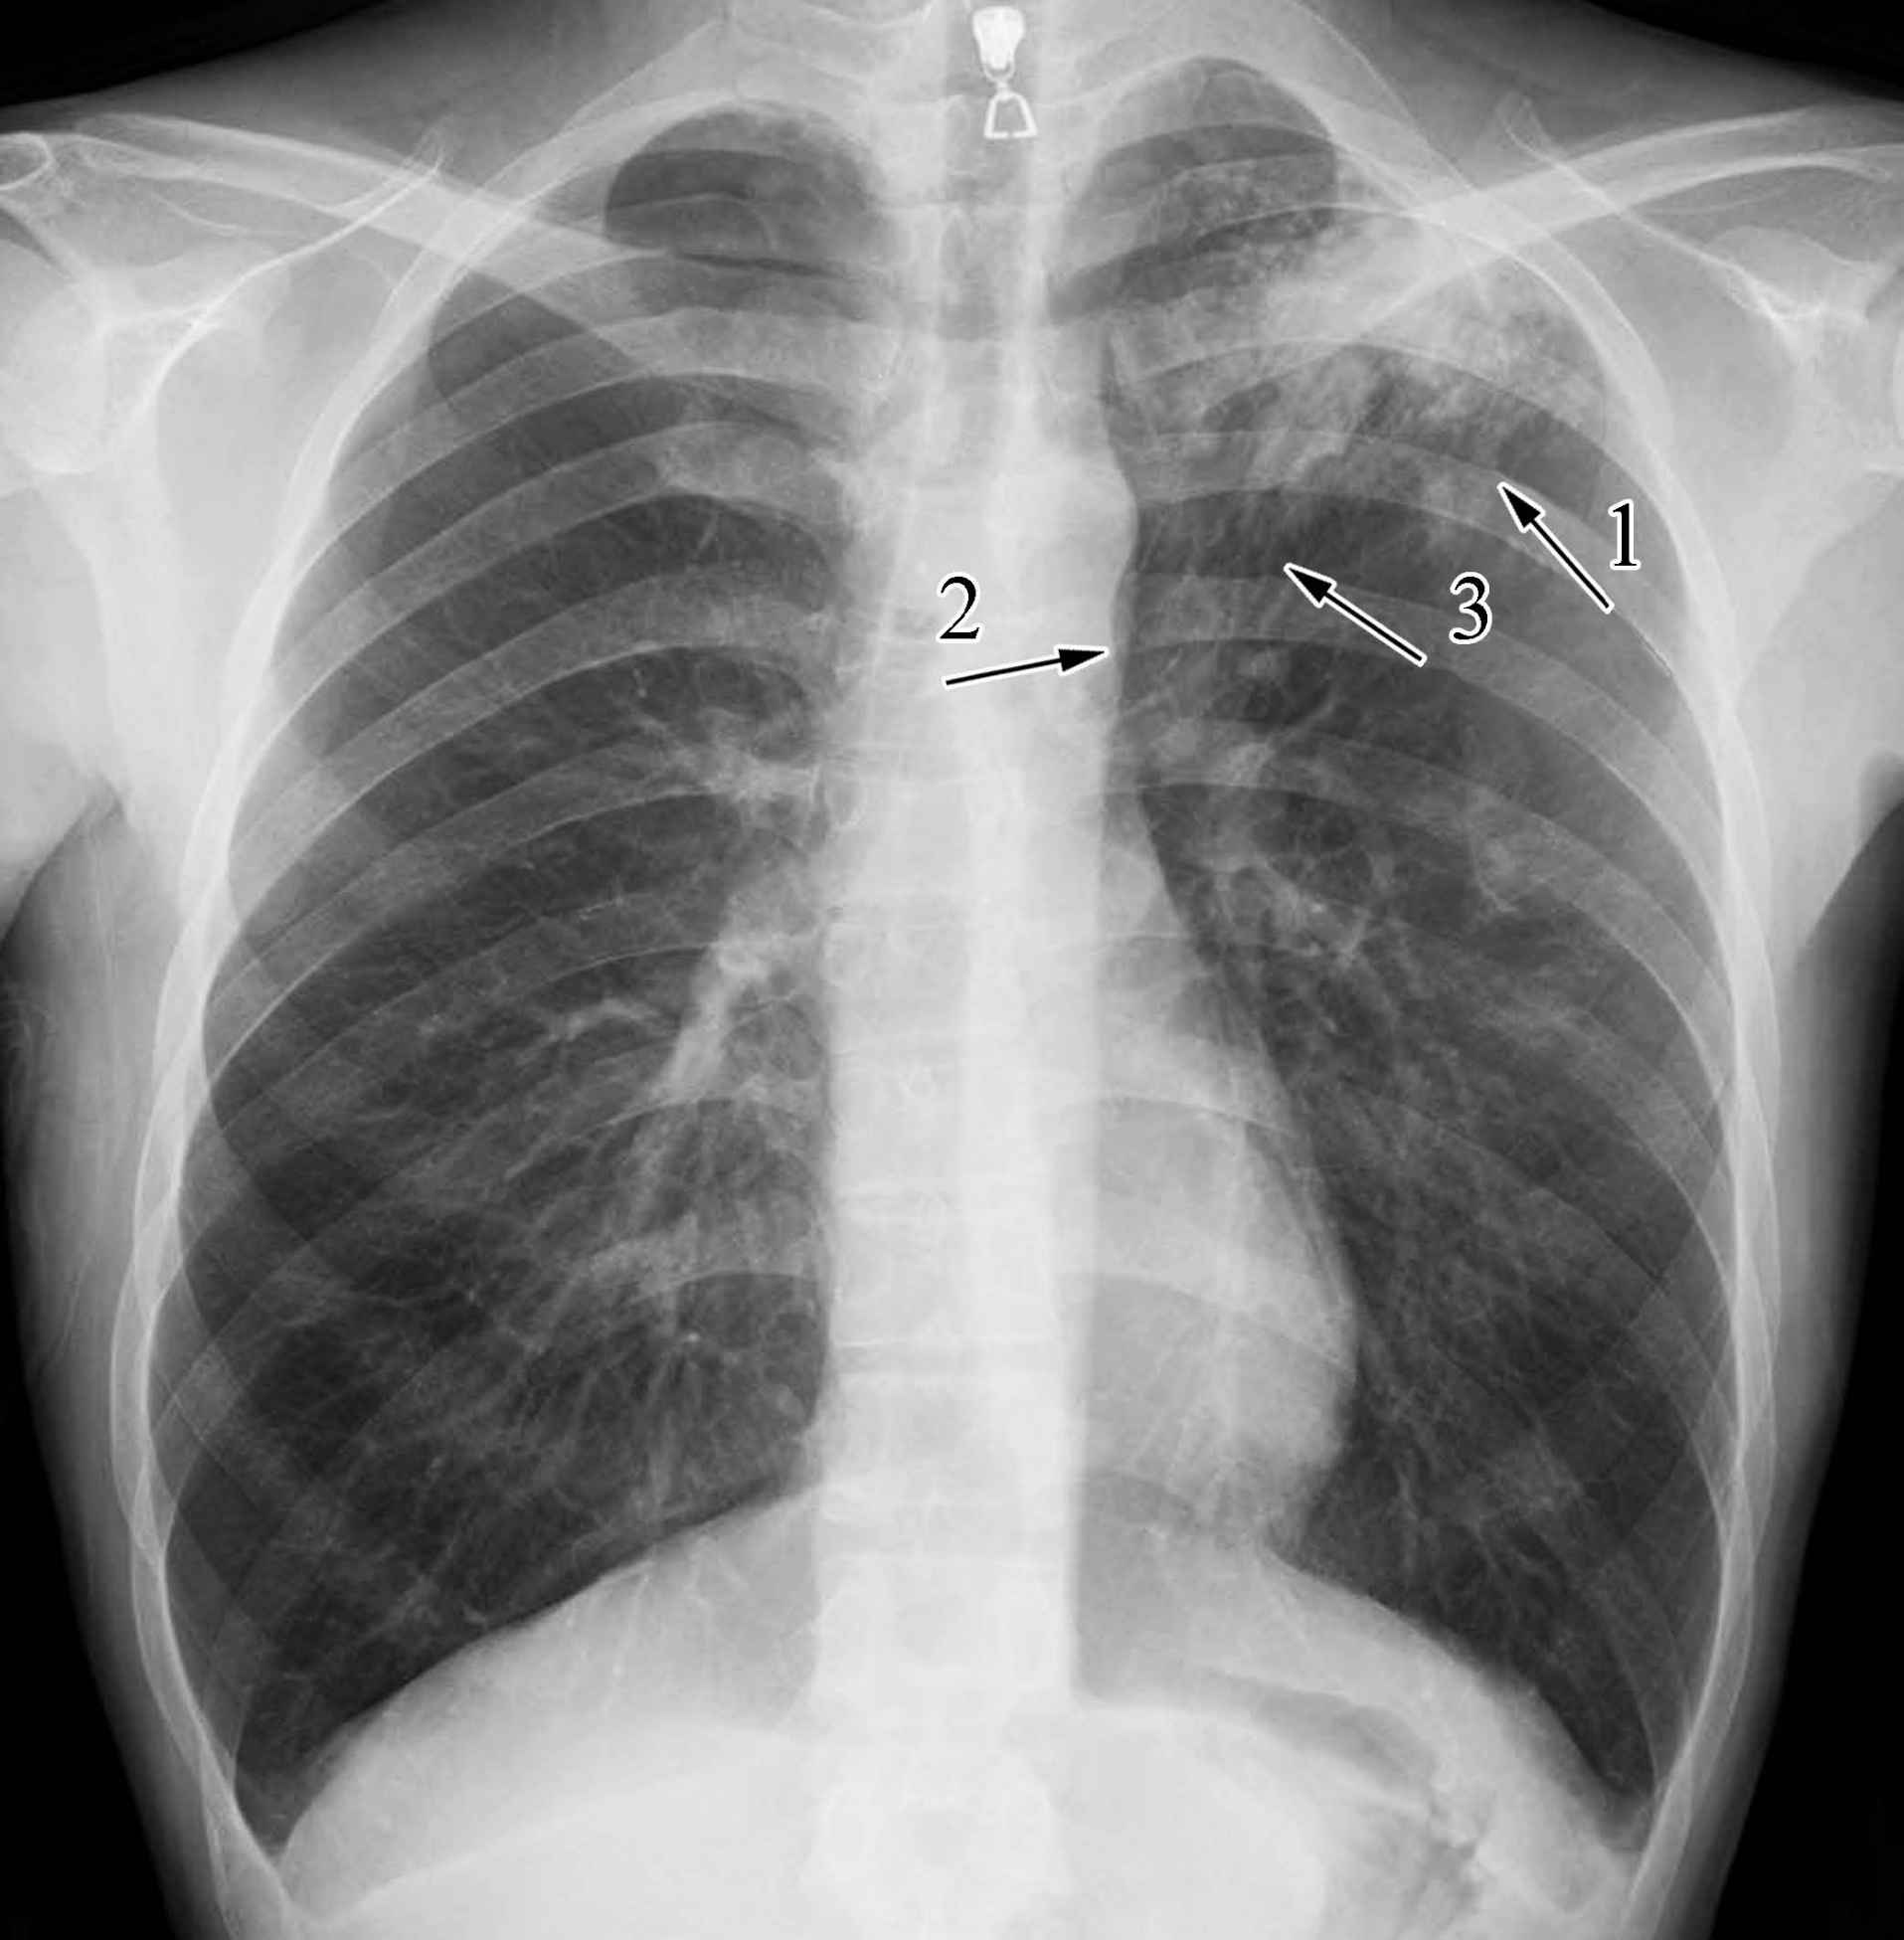
\includegraphics{./images/Image00153.jpg}
 \captionsetup{justification=centering}
 \caption{正位X线胸片示原发性肺结核}
 \label{fig3-5-1}
  \end{figure} 

\textbf{【病史摘要】}
 男性,17岁。咳嗽、咳少量白粘痰20多天,时有低热,多次验血白细胞计数稍偏高,发病初始曾抗感染治疗1周,效果不佳。

\textbf{【X线表现】}
 两肺纹理增加,左上肺见片絮状模糊影(箭头1),左肺门上部呈结节状增大(箭头2),左上肺病灶与左肺门间示多条条索状影(箭头3)。心影正常大小。

\textbf{【X线诊断】}  左上肺原发性肺结核。

\textbf{【评  述】}
 原发性肺结核(Ⅰ型)又名原发综合征,多见于儿童及青少年、少数为成人。临床上以低热、咳嗽、盗汗和消瘦为主要症状。胸片的典型表现有三个X线征象:肺内胸膜下斑片状模糊影为表现的原发浸润灶(多数位于右上肺)、肺门纵隔边缘向肺野呈球状突出为表现的肺门纵隔淋巴结肿大和在二者中间,以不规则粗索条状影相连为表现的淋巴管炎。三个X线征象同时在胸片上显示可表现为具有特征性的哑铃状影。增大的淋巴结有时可压迫支气管,引起相应肺叶的不张。原发病灶经治疗后易于吸收,少数原发病灶可以干酪样变,形成空洞。但淋巴结炎常伴不同程度的干酪样坏死,愈合较慢,愈合后可残留钙化。当原发病灶吸收后,原发性肺结核则表现为胸内或纵隔内淋巴结结核,淋巴结内部干酪灶可破溃至血管和支气管产生血行或支气管播散。

影像上本病常需与节段性肺炎、胸内结节病、淋巴瘤等相鉴别,非结核性肺炎通常肺门淋巴结不肿大或轻度肿大,结合病史和实验室检查可加以鉴别;胸内结节病及淋巴瘤引起的肺门淋巴结肿大常为双侧性,常伴支气管旁淋巴结肿大,而肺门淋巴结结核通常为单侧性,较少伴有支气管旁淋巴结肿大。再者,结节病和淋巴瘤往往有多个淋巴结肿大融合成土豆块状或团块状,边缘呈分叶状改变。CT及MRI能清晰地显示上述三个征象,优于胸片,特别是对诊断肺门及纵隔各组淋巴结有无肿大、有无外侵均可较好地显示。但这种典型的三者综合征象并不多见,一般以原发病灶及其周围炎和淋巴结炎表现最为突出,而淋巴管炎往往不易显示。此外,根据临床症状、结核接触史、结核菌素试验、白细胞计数及X线定期随诊复查才能鉴别。

\subsection{继发性肺结核}

\begin{figure}[!htbp]
 \centering
 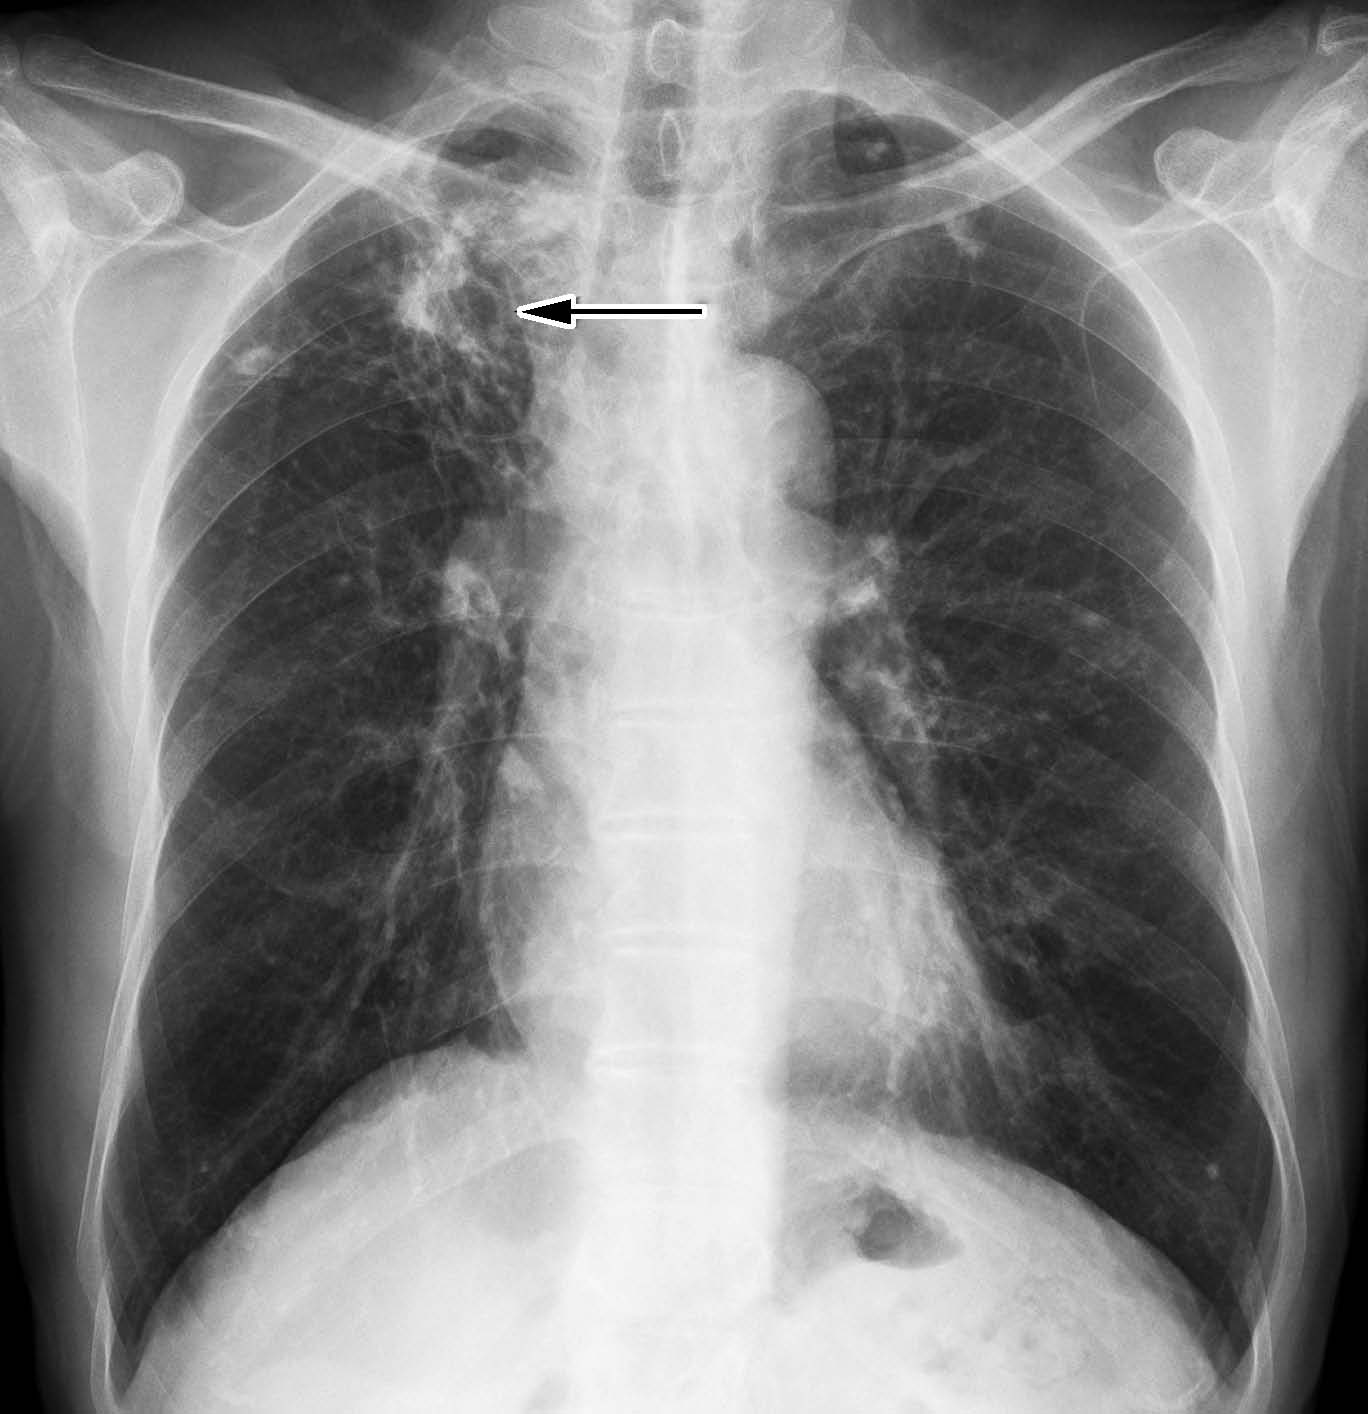
\includegraphics{./images/Image00154.jpg}
 \captionsetup{justification=centering}
 \caption{正位X线胸片示两上肺继发性肺结核}
 \label{fig3-5-2}
  \end{figure} 

\textbf{【病史摘要】}
 男性,49岁。咳嗽、咳粘痰3年伴盗汗、疲乏消瘦,有咯血3~4小口史2次,时有低热。

\textbf{【X线表现】}
 两肺纹理增多,右上肺见片状、条索状、结节状影,密度较高,片状影内见内壁光整空洞影(箭头),两肺见散在斑点及小斑块状高密度影。心影、横膈正常。

\textbf{【X线诊断】}  右肺上叶继发性肺结核。

\textbf{【评  述】}
 肺结核的基本病理变化是渗出、增殖和变质。渗出性为主的病变表现为浆液性或纤维素肺泡炎,该变化发生在病变早期,或机体免疫力低下,或菌量少却毒力强,或变态反应较强的情况下。若菌量少、毒力较低,或人体抵抗力较强,对结核杆菌产生一定免疫力时,病变则以增殖为主的结核性结节肉芽肿为特征。增殖性病变周围也可出现渗出性病变,两者常混合存在。当人体抵抗力增强或经正规抗结核药物治疗,细菌可逐渐被控制、消灭,病变可吸收、纤维化、纤维包裹或钙化。变质为主的病变多由渗出性或增生性病变发展而来,常常以菌量大、毒力强、机体抵抗力低、变态反应增高或未适当治疗时发生。细菌增殖,病灶可扩大、溶解、液化和空洞形成,并可经血行发生肺内及全身性播散,也可经支气管发生肺内播散。在上述这些病理变化过程中,不同阶段所见的X线征象不同。

肺结核的临床分类,目前以中华结核病学会于1998年制定的新的中国结核病分类为标准,共分为五类。①原发性肺结核(代号:Ⅰ型):原发性肺结核为原发结核感染所致的临床病症,包括原发综合征和胸内淋巴结结核。②血行播散型肺结核(代号:Ⅱ型):包括急性血行播散型肺结核(急性粟粒性肺结核)及亚急性、慢性血行播散型肺结核。③继发性肺结核(代号:Ⅲ型):继发性肺结核是肺结核中的一个主要类型,包括浸润型肺结核、空洞型肺结核、纤维空洞型肺结核、结核球和干酪性肺炎。④结核性胸膜炎(代号:Ⅳ型):临床上已排除其他原因引起的胸膜炎。包括结核性干性胸膜炎、结核性渗出性胸膜炎、结核性脓胸。⑤其他肺外结核(代号:Ⅴ型):其他肺外结核按部位及脏器命名,如骨关节结核、结核性脑膜炎、肾结核、肠结核等。

继发性肺结核(Ⅲ型)的临床表现不一,可无明显症状,或有低热、盗汗、疲乏、消瘦、食欲缺乏、咳嗽、咯血、胸痛和气促等。肺结核的诊断需以临床症状、影像学表现和痰菌数量为依据进行综合诊断。

继发性肺结核为成年结核中最常见的类型,病灶见于两肺锁骨上、下区是较为典型表现,肺结核的各种基本病变如渗出性病变、增殖性病灶、干酪性病灶、空洞、纤维性病灶,甚至钙化灶及结核球形成等多种不同性质的病变都可出现。就同一个患者来讲,X线表现多种多样,有时可以一种为主或多种征象混合并存。以本例患者X线表现上就可看出,右上肺病灶主要为增殖、空洞病变和纤维、钙化灶。说明Ⅲ型肺结核的X线表现可多种多样,可以一种为主或多种征象混合并存。

浸润型肺结核,渗出为主的需与肺炎特别是肺炎支原体肺炎鉴别;大片的干酪性肺炎需与肺脓肿鉴别;结核空洞主要与癌性空洞鉴别,有时亦会与肺大疱混淆;至于结核球需与周围型肺癌、球形肺炎等相鉴别。

\subsection{继发性肺结核(浸润型肺结核)}

\begin{figure}[!htbp]
 \centering
 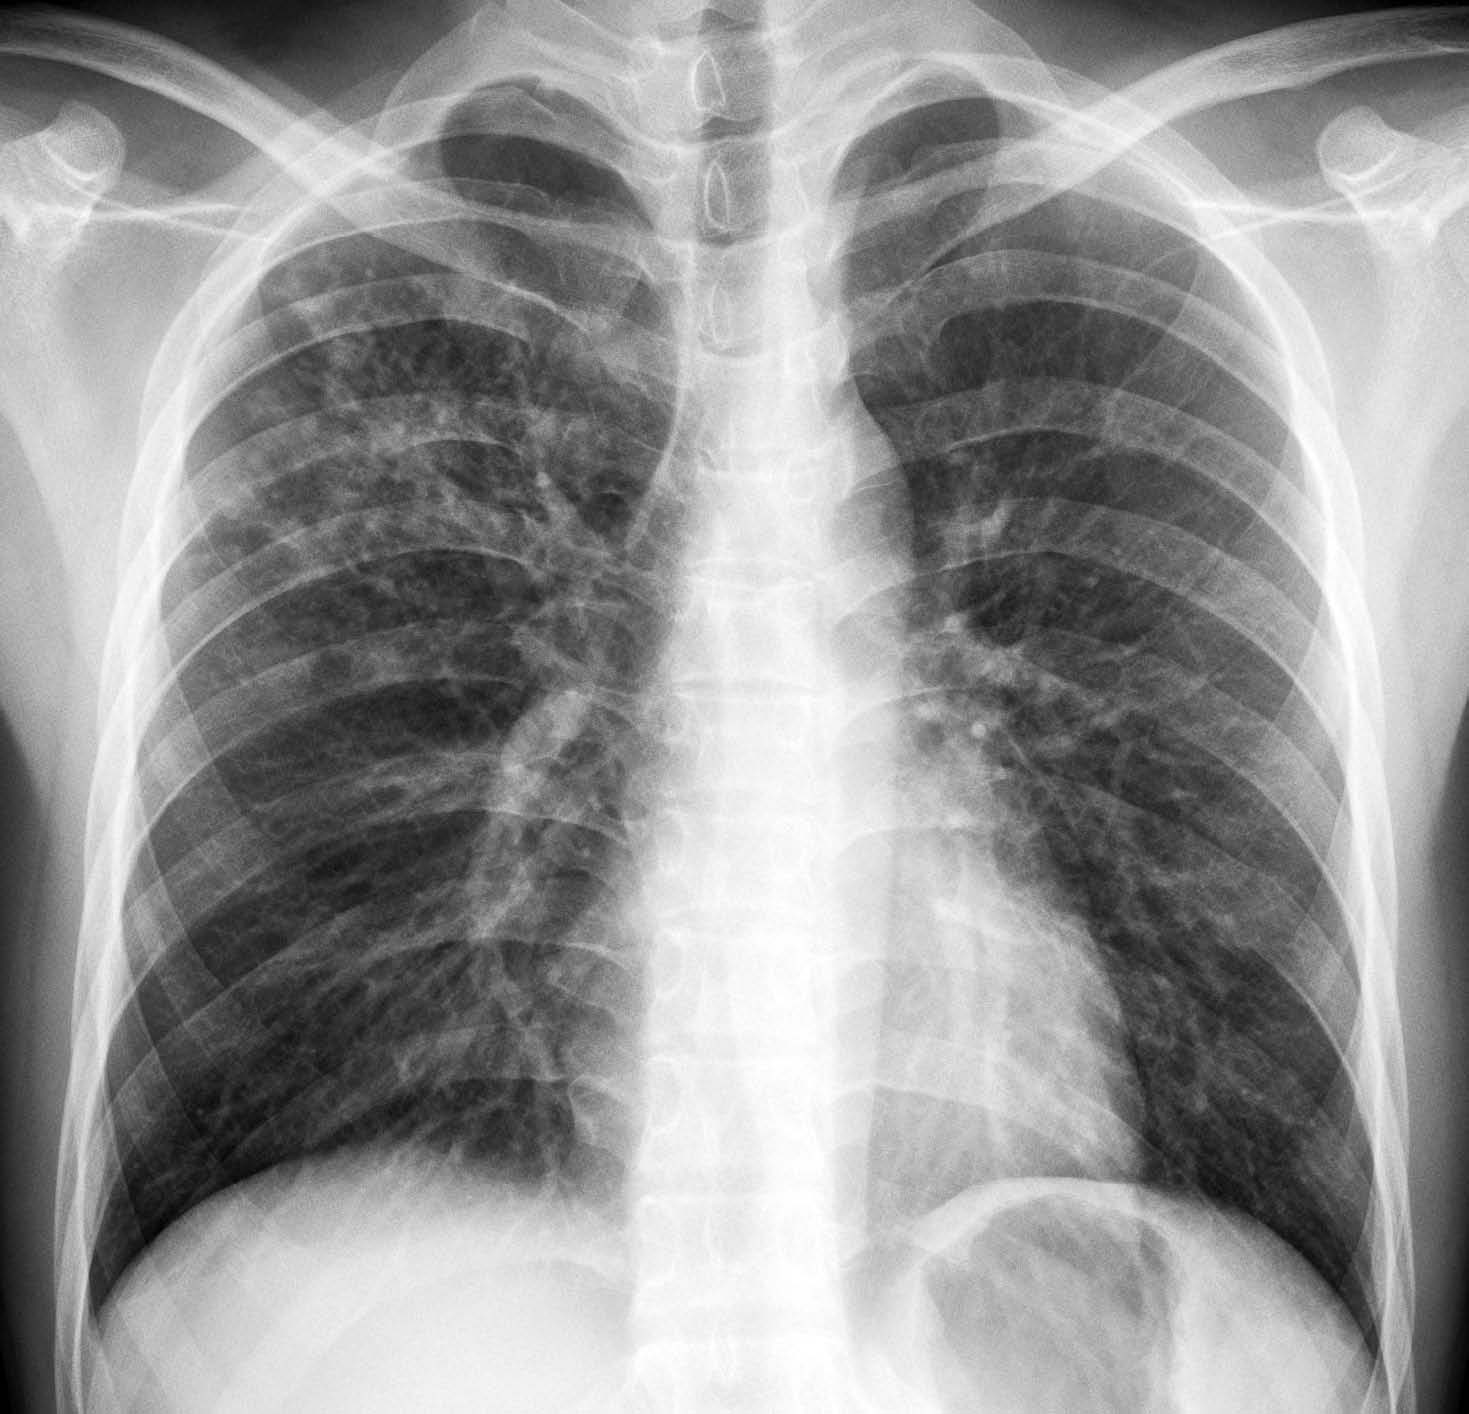
\includegraphics{./images/Image00155.jpg}
 \captionsetup{justification=centering}
 \caption{正位X线胸片示右上肺浸润性肺结核}
 \label{fig3-5-3}
  \end{figure} 

\textbf{【病史摘要】}
 男性,26岁。咳嗽、咳痰1个月余,痰不多,为白色粘痰,偶有低热,夜间有盗汗,无胸痛。体格检查:一般情况可,心肺听诊无异常发现。

\textbf{【X线表现】}
 两肺纹理增加,右上肺见斑点状、小斑片状影聚集,阴影边缘模糊,两肺门影正常。心影、横膈正常。

\textbf{【X线诊断】}  右上肺Ⅲ型结核(浸润型肺结核)。

\textbf{【评  述】}
 浸润型肺结核多为已静止的原发病灶的重新活动,或为外源性再感染。由于机体对结核菌已产生特异性免疫力,病变常局限于肺的一部,多在肺上叶尖段、后段及下叶背段。

X线表现多种多样,可以一种为主或多种征象混合并存,主要可见以下8种征象:①局限性斑片阴影:见于两肺上叶尖段、后段和下叶背段,右侧多于左侧。②大叶性干酪性肺炎:为一个肺段或肺叶呈大片致密性实变,密度中心较高,边缘模糊。③增殖性病变:呈斑点状阴影,边缘较清晰,排列成梅花瓣或树芽状阴影,为结核病的典型表现。④结核球:圆形、椭圆形阴影,大小0.5~4cm不等,常见2~3cm,边缘清晰,轮廓光滑,偶有分叶,密度较高,内部常见斑点、层状或环状钙化。结核球周围常见散在的纤维增殖性病灶,称卫星灶。⑤结核性空洞:圆形或椭圆形病灶内见透亮区。空洞壁薄,内壁一般较规则,有时可呈厚壁不规则空洞。常见一条或数条粗大条状阴影与空洞相连,表示引流大气管与空洞相通。⑥支气管播散病变:结核空洞干酪样物质经引流支气管排出,引起同侧或对侧的支气管播散。表现为沿支气管分布的斑片状阴影,呈腺泡排列,或相互融合成小叶阴影。⑦硬结钙化:增殖性病灶好转后可有钙盐沉着,病灶呈边缘锐利的高密度影,完全钙化者,呈骨样密度的斑片状或小块状阴影。致密阴影长期无变化,表现结核病痊愈。钙化也可产生在支气管壁或胸膜以及淋巴结内。⑧小叶间隔增厚:表现为索条及网状阴影。本例患者以局限性渗出性病灶为主。

浸润型肺结核患者体质情况一般较弱,痰结核菌常呈阳性,肺内阴影实变区密度不均匀,常可见小空洞,病变肺叶体积一般有缩小,其他肺野有播散病灶,短期复查病变不吸收,这些特征有助于与细菌性肺炎相鉴别。机化性肺炎的病变形态极不规则,病变边缘常有多数粗大的长毛刺向肺野伸展,并常可见部分边缘模糊不清,周围肺野没有播散病灶,所在肺叶常因纤维化而收缩,附近胸膜常有明显的增厚,易与浸润型肺结核区别。

常规X线胸片可以解决肺结核的大部分诊断问题。CT扫描可以发现胸片难以显示的隐蔽性病灶,并可提供结核病灶的内部细节,有助于鉴别诊断。肺结核治疗后的复查,摄胸片简单、经济,应为其随访的主要检查方法。

\subsection{继发性肺结核(慢性纤维空洞型肺结核)}

\begin{figure}[!htbp]
 \centering
 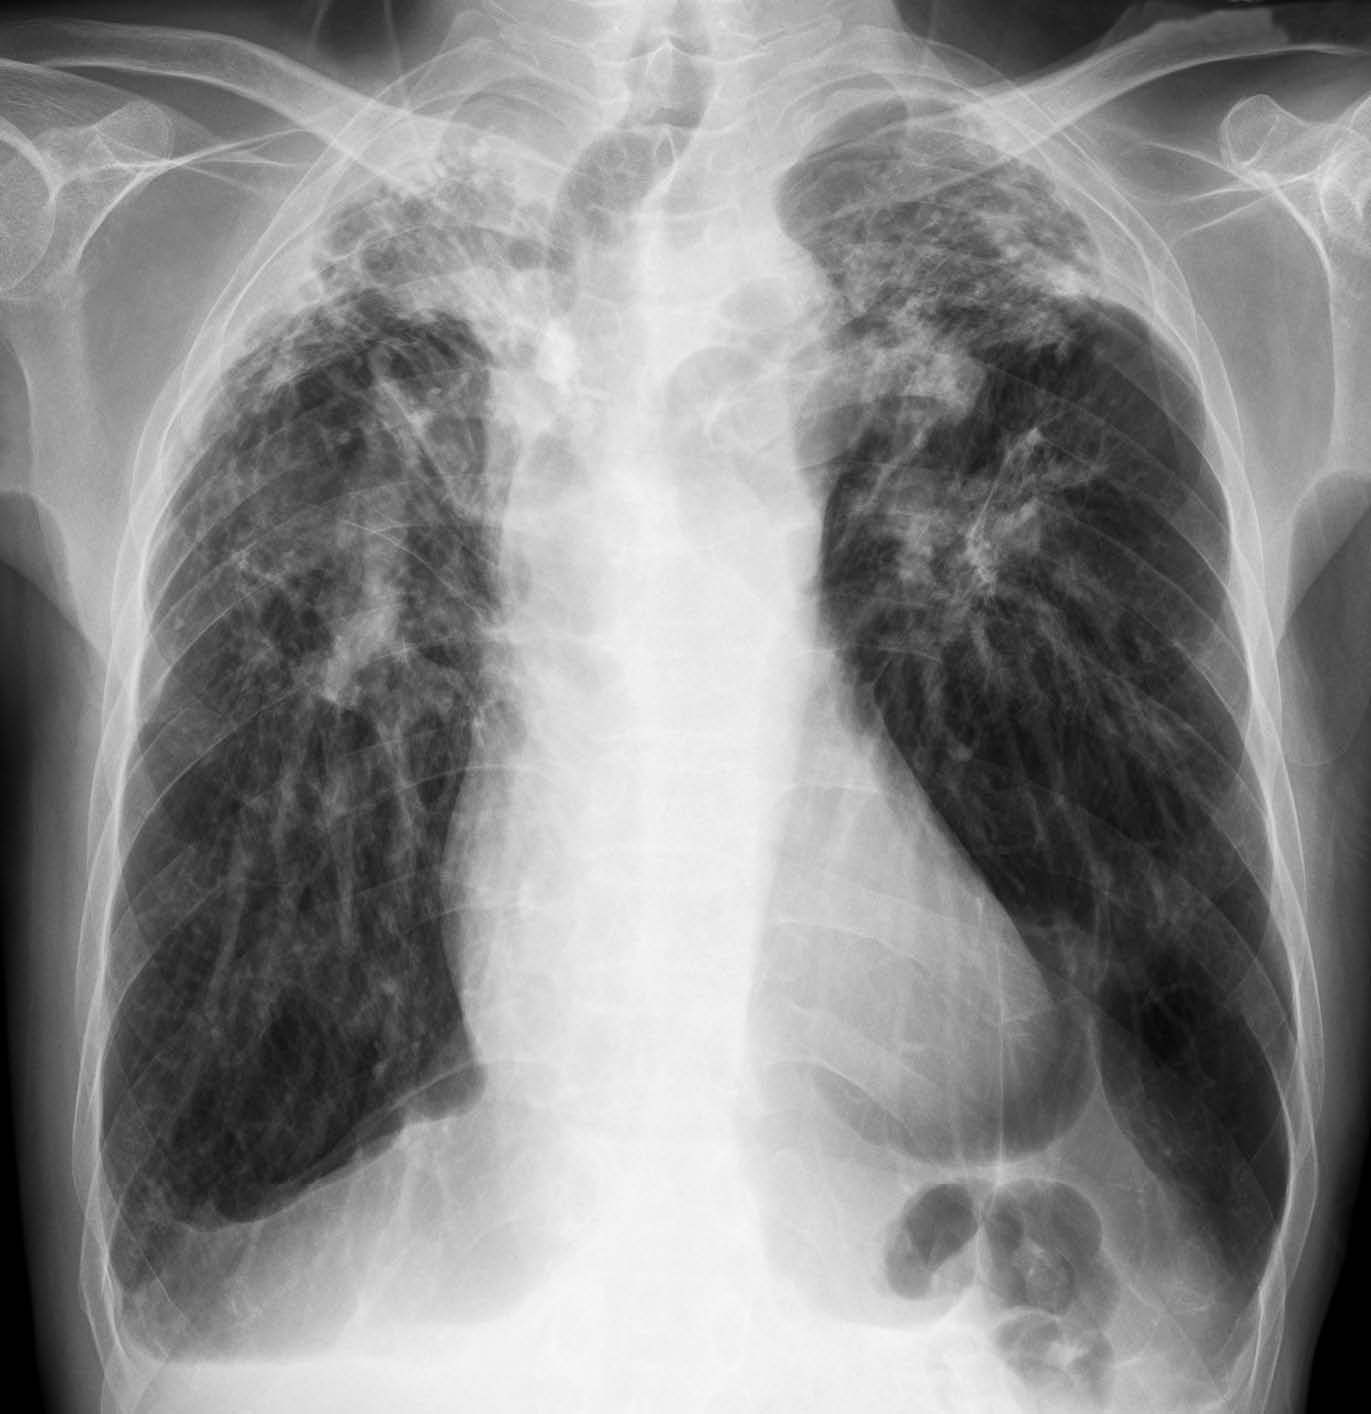
\includegraphics{./images/Image00156.jpg}
 \captionsetup{justification=centering}
 \caption{正位X线胸片示两上肺呈慢性纤维空洞性肺结核}
 \label{fig3-5-4}
  \end{figure} 

\textbf{【病史摘要】}
 男性,58岁。反复咳嗽、咳痰近20年,有多次少量咯血史,时有盗汗、低热,自述有“肺结核”病史。

\textbf{【X线表现】}
 正位X线片示两上肺大片状模糊影,病灶密度高低不均,内见不规则透亮区,病灶下缘有大量纤维索条状影;双肺上叶收缩,两侧上胸部肋间隙变窄,双肺门上抬,肺纹理紊乱,呈垂柳状;右肺中野见小斑点状模糊影;上纵隔、气管牵拉右移,邻近胸膜增厚明显;两上肺病灶内见斑点状钙化影,左上肺病灶内见结节状、边界清、密度较高影;下部胸廓肋间隙增宽,双膈变平下降,呈桶状胸等肺气肿表现;双侧部分胸膜增厚及粘连。心影属正常。

\textbf{【X线诊断】}  继发性肺结核(慢性纤维空洞型肺结核)。

\textbf{【评  述】}
 本病属于继发性肺结核晚期类型,肺组织受结核病灶破坏,形成慢性纤维空洞,肺内有多种不同性质的病变,病程达数年或数十年之久。是由于未经彻底治疗,病变恶化,反复进展演变而来。

结核空洞的主要症状为慢性咳嗽、咳痰、反复咯血和痰结核菌阳性,有急性支气管播散时可有急性中毒症状和呼吸道症状。净化空洞无症状,痰结核菌阴性。

慢性纤维空洞型肺结核是各型肺结核经久不愈、反复恶化的结果,其病变为一个或数个纤维厚壁空洞及周围肺组织大量纤维增生,同时有牵拉性支气管扩张、胸膜增厚、支气管播散、肺气肿等继发改变等。主要X线表现:①单侧或双侧肺上中部不规则透亮区。②空洞壁厚,壁周围有大量纤维粘连,使洞壁固定而坚硬。③多支引流支气管与空洞相通,呈索条轨道状阴影。④空洞周围有大片渗出和干酪病变,也可见不同程度的钙化。⑤双肺上叶收缩,双肺门上抬,肺纹理紊乱,呈垂柳状。⑥双肺中下叶透亮度增加。⑦纵隔变窄,呈滴状心。⑧肋间隙增宽,双膈变平下降,呈桶状胸等肺气肿,甚至肺心病的表现。⑨胸膜增厚及粘连。⑩常见支气管播散性结核病灶。本例患者的X线表现,慢性纤维空洞性肺结核的10种主要X线表现基本都具有。

结核性空洞与癌性空洞常需鉴别,结核性空洞通常空洞壁薄,壁内、外缘较光滑,空洞周围常有不同性质的结核病灶。癌性空洞由肿瘤发生坏死液化后形成,多为厚壁空洞,常为偏心脏,外壁多呈分叶状,可有毛刺,壁内缘多高低不平,有结节状突起,邻近胸膜正常或有胸膜凹陷现象。进一步CT检查有利于观察空洞内部详细情况,以及洞壁强化程度,可做出鉴别诊断。

\subsection{继发性肺结核(空洞型肺结核)}

\begin{figure}[!htbp]
 \centering
 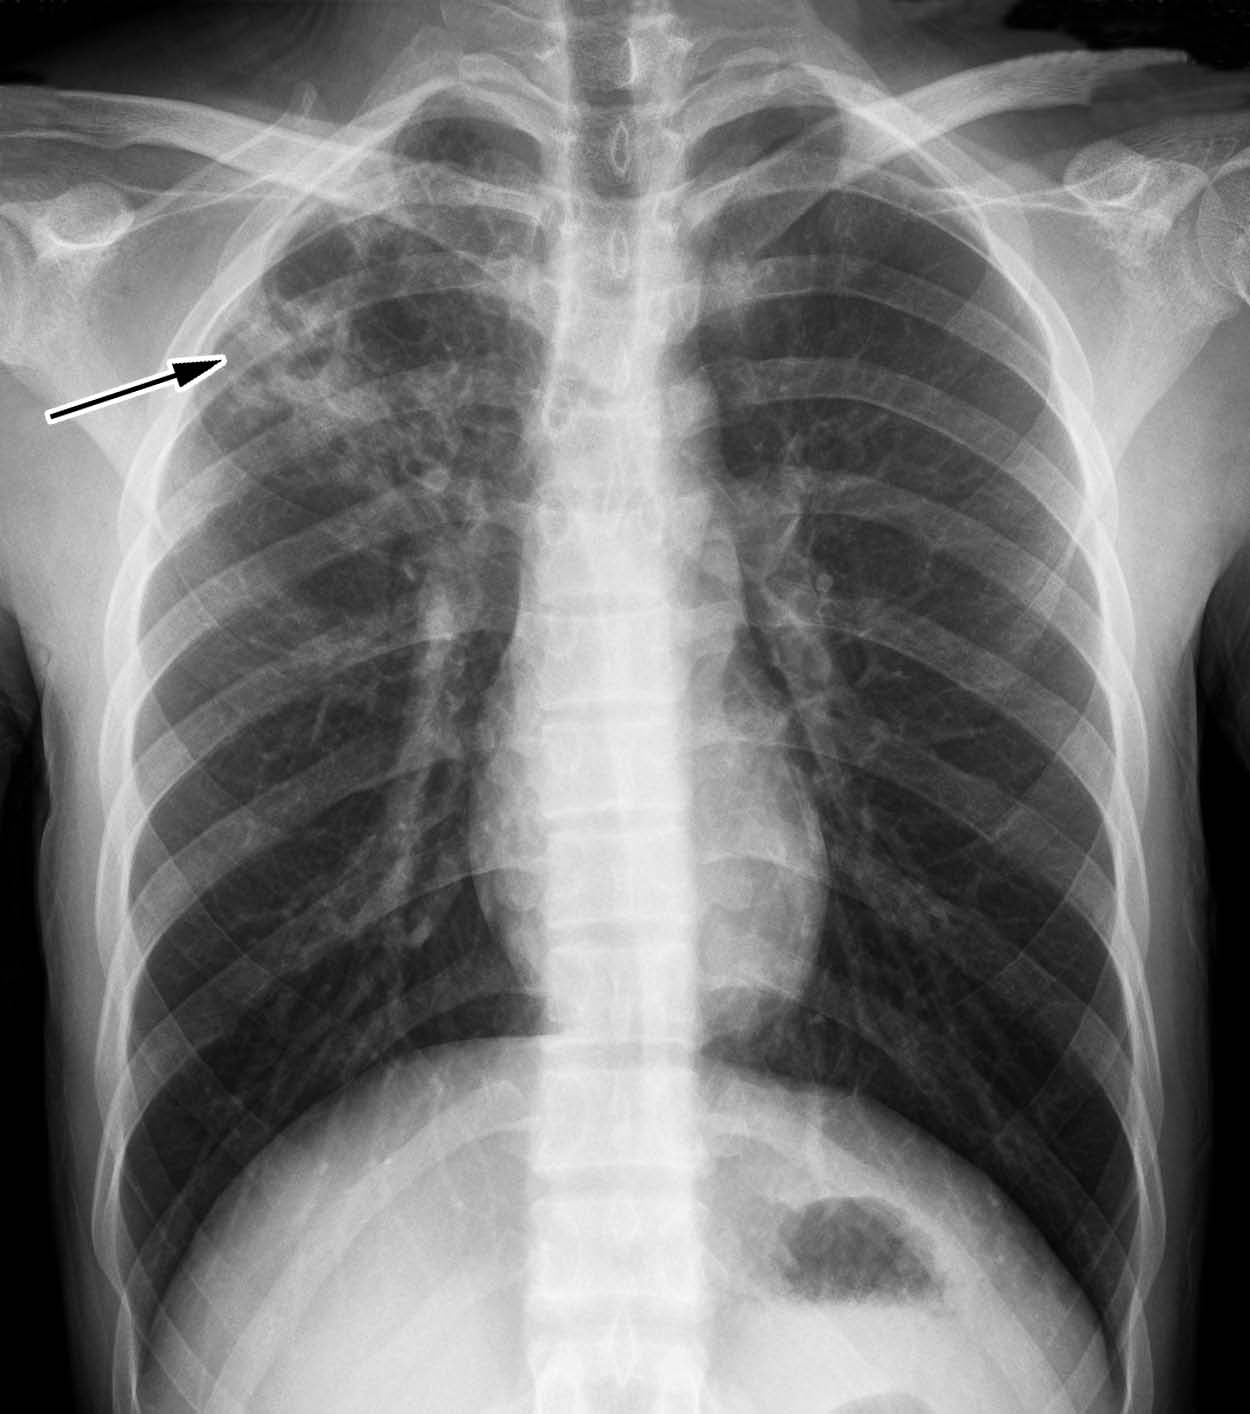
\includegraphics{./images/Image00157.jpg}
 \captionsetup{justification=centering}
 \caption{正位X线胸片示右上肺继发性肺结核(空洞型肺结核)}
 \label{fig3-5-5}
  \end{figure} 

\textbf{【病史摘要】}  男性,24岁。咳嗽、咳痰数天,咯血数口1天。

\textbf{【X线表现】}
 右上肺大片状模糊影,内见洞内壁光整不规则形空洞影,空洞周围有斑片状影及条索状影,两肺门大小正常。心影正常。

\textbf{【X线诊断】}  右上肺继发性肺结核(空洞型肺结核)

\textbf{【评  述】}
 结核空洞为干酪坏死液化排空而成,空洞壁主要由三层病理结构组成,内层为干酪物质,中层为结核性肉芽组织,外层为纤维组织。各种类型的空洞其三层结构多少不一,无壁或虫蚀样空洞主要见于急性干酪性肺炎,空洞壁主要由干酪物质构成。薄壁空洞的洞壁厚度小于3mm,主要由纤维和肉芽组织构成,干酪物质较少;如以纤维组织为主,则为纤维薄壁空洞。干酪厚壁空洞的洞壁主要由干酪物质构成,纤维和肉芽组织较少;纤维厚壁空洞的洞壁在3mm以上,主要为纤维组织构成。张力空洞主要由引流支气管活瓣性阻塞所致,空洞壁以纤维和肉芽组织为主,净化空洞则由支气管粘膜上皮长入空洞内而构成洞壁的内层,外层为纤维组织。结核空洞的主要症状为反复咯血和痰结核菌阳性。

主要X线表现常好发于上叶尖后段和下叶背段,但也可见于两肺的任何部位;空洞内一般无液平,或仅有少量液体;空洞周围有卫星病灶;常可见引流支气管;短期观察可无明显变化。

肺结核的影像学表现复杂繁多,结合病史、影像学表现的特点以及痰液检查结果,一般不难做出诊断。但不同性质的病变与其他非结核病变有相似之处,应注意鉴别。结核性空洞与癌性空洞的鉴别见上节内容。急性肺脓肿空洞壁厚且较均匀;空洞外缘模糊,有较广泛的炎性浸润;空洞内缘毛糙不整或光整;空洞内常有宽厚的液平面;周围无卫星病灶;抗炎治疗后,可在短期内吸收缩小。慢性肺脓肿空洞常呈多房或有分隔;空洞形态不整,有时部分边缘显示不清;空洞常为薄壁,但部分可因炎性浸润而模糊;病变可跨过叶间裂;周围一般无卫星病灶。含气或液气囊肿的空洞形态很规则,一般为圆形;空洞壁甚薄,厚薄一致;空洞内外缘光整;感染时空洞内常有液体;空洞周围无卫星病灶,远处无播散病灶。

\subsection{继发性肺结核(结核球)}

\begin{figure}[!htbp]
 \centering
 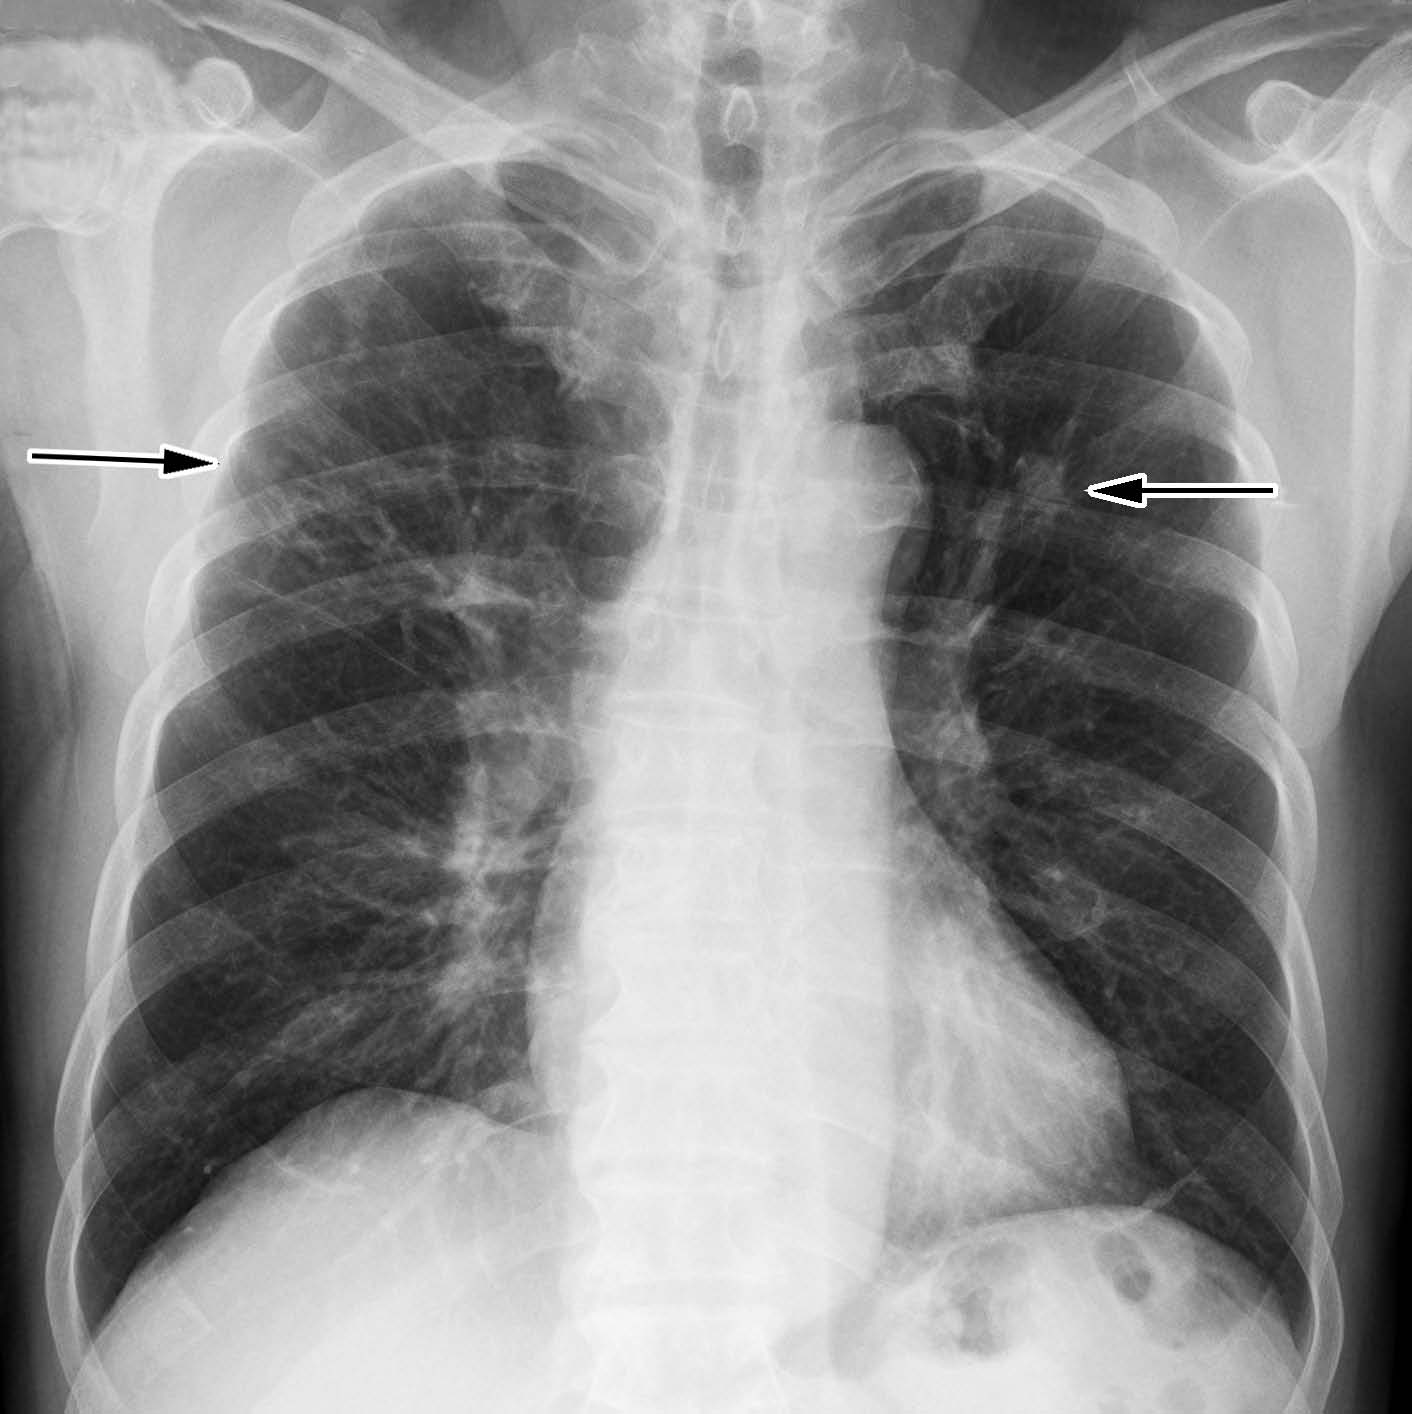
\includegraphics{./images/Image00158.jpg}
 \captionsetup{justification=centering}
 \caption{正位X线胸片示两上肺继发性肺结核,左上肺结核球}
 \label{fig3-5-6}
  \end{figure} 

\textbf{【病史摘要】}
 男性,75岁。间断性咳嗽7~8年,加重3天,咳时少痰,无咯血,无胸痛。体格检查:两肺呼吸音粗,未闻及干湿性啰音。心音正常。

\textbf{【X线表现】}
 两肺纹理增加,右肺上叶见多发条索状影及小片状影;左肺上叶见较高密度结节状影,边缘清晰但欠整齐,周围有柔软条带状影;余肺野未见异常密度影,主动脉影增宽迂曲,心影大小正常。

\textbf{【X线诊断】}
 两上肺继发性肺结核,左上肺结核球形成。主动脉硬化。

\textbf{【评  述】}
 结核球又称结核瘤,是被纤维组织包围的结核性干酪病变,直径大于2cm者称为结核球。结核球最常见为大片渗出干酪性炎症,或多个干酪渗出性小病灶融合,而被纤维组织包围或结核空洞阻塞脓液凝结而成;亦可为结核性肉芽组织部分干酪坏死被包围而成。其内主要为干酪物质,亦可为结核性肉芽组织;常有钙化及液化溶解区,包膜常完整,但亦可不完整。为浸润型肺结核的一种特殊类型,常无明显临床症状。

X线表现为好发于上叶尖后段和下叶背段,亦可发生于任何肺段;孤立球形病灶,圆形或卵圆形,通常轮廓清楚锐利;有时环绕着一层1~2mm宽度的线条包膜阴影,这是良性病变较为可靠的征象;病灶密度较高,有时其内见钙化,呈层状或米花糖样钙化有重要诊断意义;有时有浅分叶外观,病灶内甚至可形成空洞;病灶周围有散在卫星病灶;相邻胸膜常有增厚钙化;在结核球通向肺门的区域有时可见增租的肺纹理和条索影,但一般无淋巴结肿大。结核球是相对稳定的病灶,可长期保持静止状态,但当机体抵抗力降低时,病灶可恶化进展。

结核球与周围性肺癌有鉴别意义,周围性肺癌在X线胸片上常有分叶征、毛刺征及肺门纵隔淋巴结肿大。尚需与肺炎性假瘤相鉴别,肺炎性假瘤无一定好发部位;边缘更为光滑锐利;密度均匀一致,无钙化与空洞;周围无卫星病灶。CT增强检查有助于结核球与肺内其他病灶的鉴别,结核球的强化程度不如肺内恶性肿瘤,常小于20HU,且表现为环形强化,中心干酪样坏死不强化而呈相对低密度,如有肺门纵隔淋巴结肿大,肿大的淋巴结也呈环形强化。痰细胞学检查、免疫学检查、支气管镜检查和CT定位穿刺活检可以确立诊断。

\subsection{继发性肺结核(干酪性肺炎)}

\begin{figure}[!htbp]
 \centering
 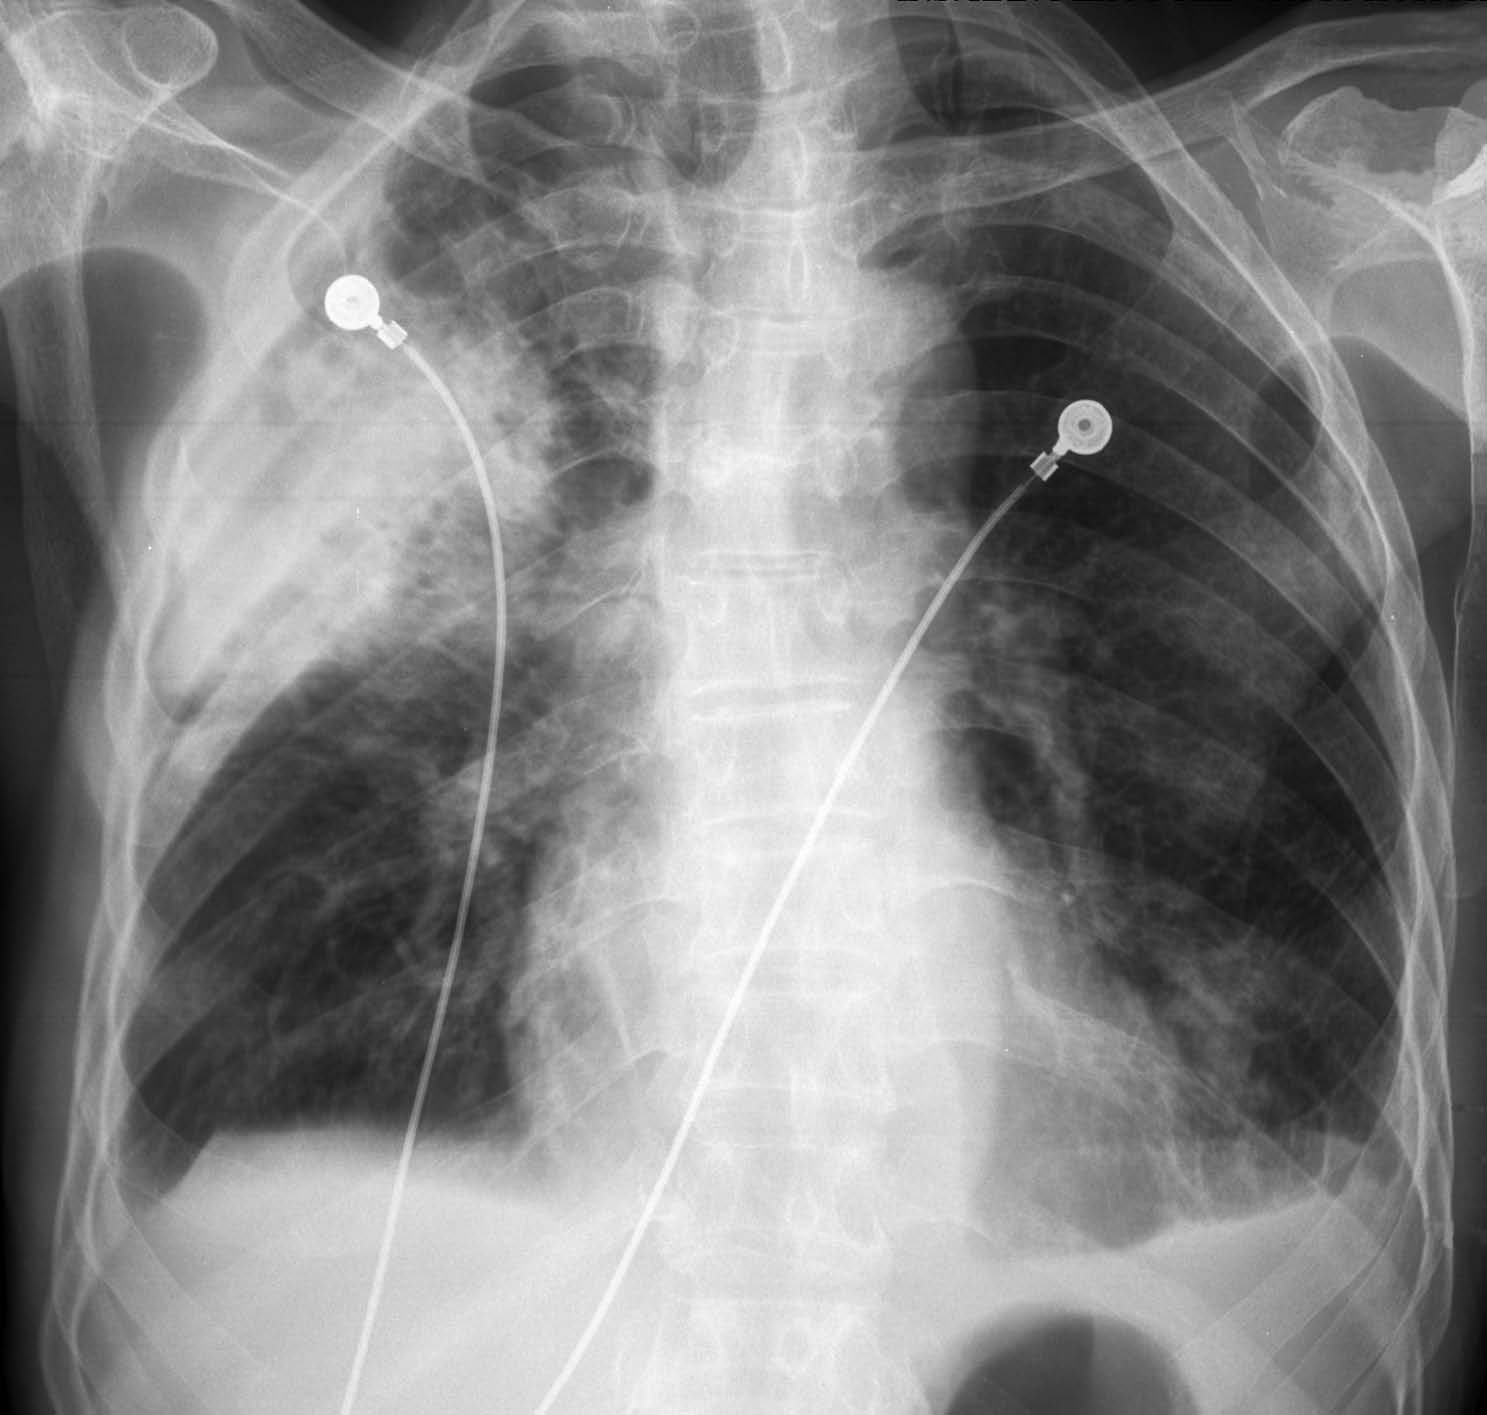
\includegraphics{./images/Image00159.jpg}
 \captionsetup{justification=centering}
 \caption{正位X线胸片示右上肺及左下肺继发性肺结核(干酪性肺炎)}
 \label{fig3-5-7}
  \end{figure} 

\textbf{【病史摘要】}
 男性,76岁。反复咳嗽、咳少量粘痰10年,胸闷气喘20多天,咯血4天,每天1~2次,每次2~3口,色鲜红,自觉发热,否认有结核病史。体格检查:一般情况可,贫血貌。两肺呼吸音粗,左下肺闻及湿性啰音;心脏听诊正常,心界不大。

\textbf{【X线表现】}
 两肺纹理增多紊乱,右上肺见大片状高密度影,病灶边缘模糊,内见多枚大小不等的无壁空洞影,呈虫蚀样;左下肺见片状淡密度模糊影。余肺野透亮度增加,两侧横膈低平,两侧肋膈角变钝。心影正常。

\textbf{【X线诊断】}
 右上肺及左下肺继发性肺结核(干酪性肺炎);两肺肺气肿改变;双侧下胸膜粘连,双侧少量胸腔积液。

\textbf{【评  述】}
 干酪坏死是结核病特有的病理变化,大量结核菌进入和(或)机体抵抗力降低时,发展成为大叶性干酪肺炎,整个大叶或肺段呈急性结核性渗出和干酪坏死,其中有大小不等的无壁空洞。干酪物质经支气管播散引起小叶性干酪肺炎,形成多数小叶发生渗出和干酪坏死。肺组织的大块干酪坏死而无明显纤维包膜,形成不规则的团块性干酪坏死,干酪病灶被纤维组织包围或为空洞阻塞脓凝时,其直径小于2cm者,为纤维干酪病灶,大于2cm者则称结核球。

干酪性肺炎的临床症状极为严重,有高热、盗汗、虚脱等严重的结核中毒症状和咳嗽、咳脓痰并咳出干酪样物质,痰内可查到大量结核杆菌,团块样干酪坏死和纤维干酪病灶可无明显临床症状。

X线表现因其累及肺实质范围的不同而分为大叶性干酪肺炎和小叶性干酪肺炎。前者为整个肺叶或肺段实变;早期密度可均匀,但很快坏死溶解形成多数不规则的虫蚀样空洞;肺叶体积常因肺组织广泛破坏而缩小;其他肺野可有支气管播散病灶;短期复查无明显变化。后者为散在的肺小叶实变;肺内常有大叶性干酪肺炎和(或)一个或几个空洞存在;病灶沿支气管呈肺段分布,呈支气管肺炎形状,但并不局限于某一个肺段,可广泛分布于一侧或两侧,以下肺多见;病灶中常有大小不一的不规则空洞;病变发展迅速,但吸收较慢。

干酪性肺炎患者体质一般较弱,痰结核菌阳性,实变区密度不均匀,常可见蜂窝样空洞,病变肺叶体积一般有缩小,其他肺野有播散病灶,短期复查病变不吸收,这些特征可与肺炎球菌肺炎相鉴别。有时尚需与机化性肺炎相鉴别,后者病变形态常极不规则;病灶边缘常有多数粗大的长毛刺向肺野伸展,并常可见部分边缘模糊不清;周围肺野没有播散病灶;所在肺叶常因纤维化而收缩,附近胸膜常有明显的增厚。

\subsection{急性粟粒性肺结核}

\begin{figure}[!htbp]
 \centering
 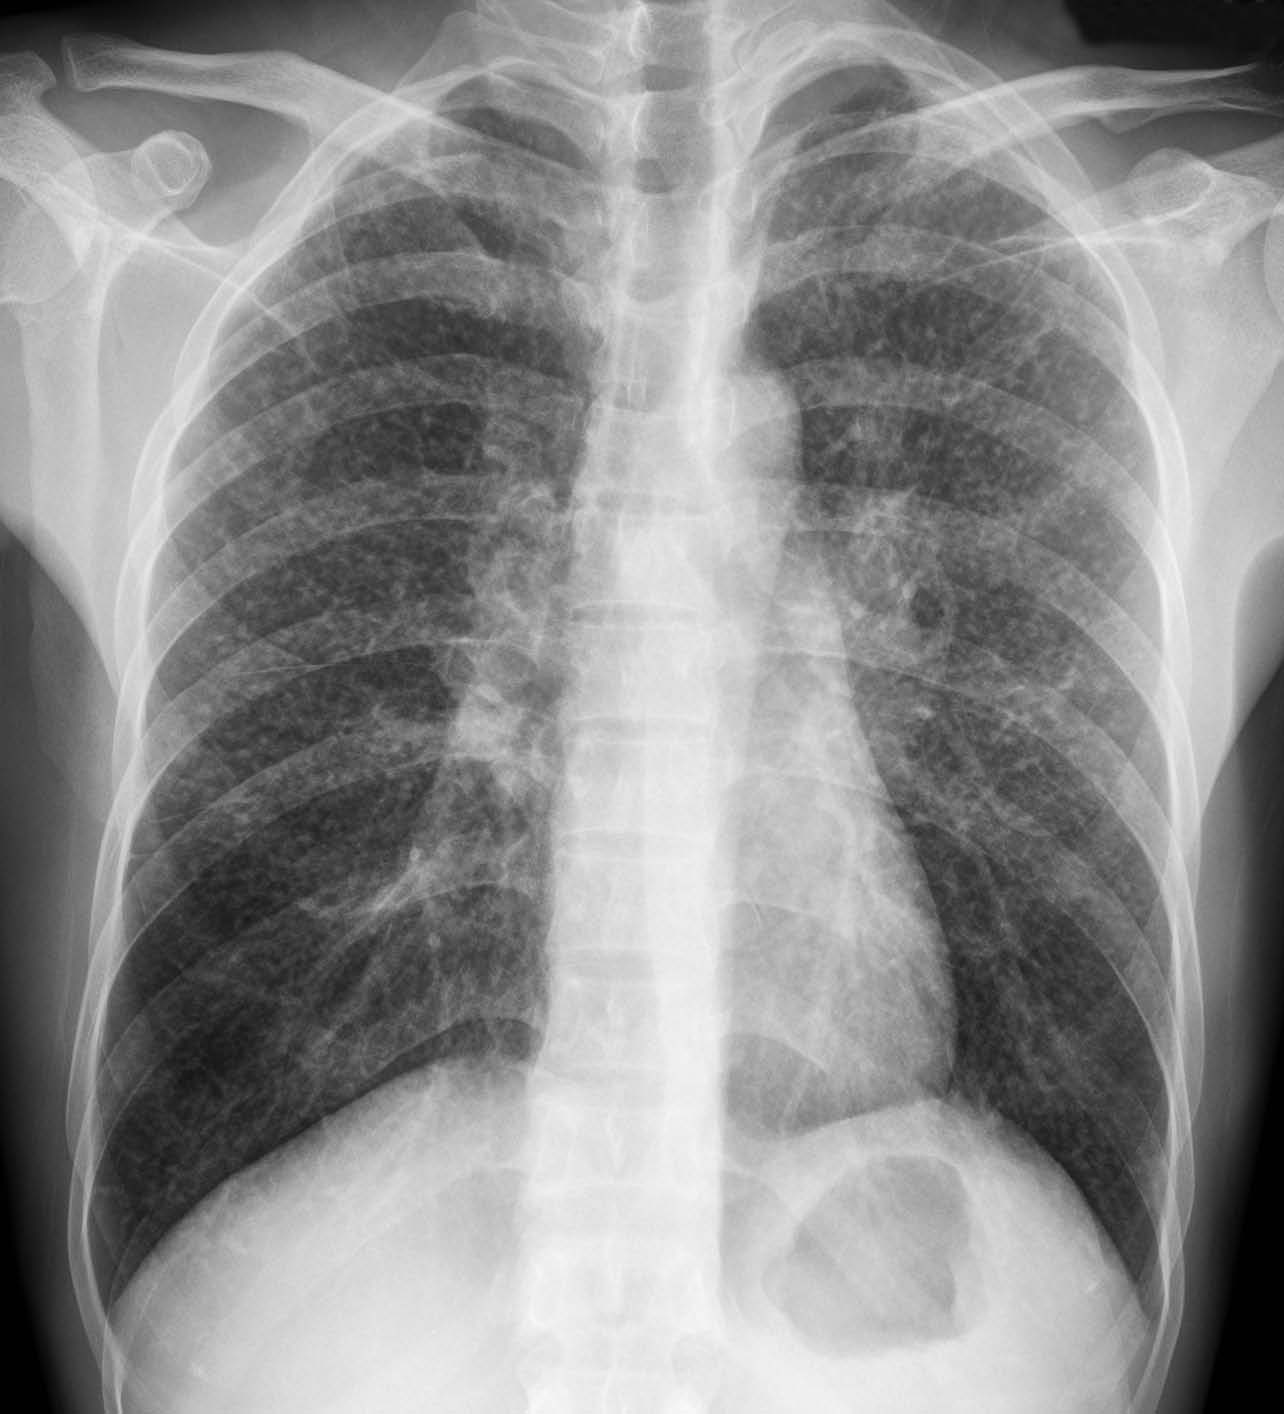
\includegraphics{./images/Image00160.jpg}
 \captionsetup{justification=centering}
 \caption{急性粟粒性肺结核}
 \label{fig3-5-8}
  \end{figure} 

\textbf{【病史摘要】}
 男性,40岁。咳嗽、咳痰1个月余,发热4天,痰涂片抗酸染色(+++)。

\textbf{【X线表现】}
 双肺野自肺尖至肺底见弥漫性粟粒状致密影,边界欠清晰,诸小结节大小、密度、分布均匀。双侧肺门似轻度增大。心脏形态大小未见明显异常。双侧肋膈角稍钝。

\textbf{【X线诊断】}
 急性粟粒性肺结核可能性大,伴双侧肺门淋巴结可疑增大及双侧胸腔少量积液。

\textbf{【评  述】}
 本病是由于大量结核杆菌一次侵入血循环所引起,以原发性肺结核较为多见。急性粟粒性肺结核患者往往发病急剧,结核中毒症状较明显。本例患者是在原发性肺结核引起血行播散后,症状突然加剧。双肺见广泛针尖或粟粒状大小致密影,粟粒大小为1~2mm,边缘清晰,呈三个一致:即分布一致、大小一致和密度一致,与支气管走行无关,此乃急性粟粒性肺结核的特征性X线表现。

双肺弥漫性粟粒性阴影可由很多疾病引起。根据病史,包括职业史、生活史等即可排除许多疾病。急性粟粒性肺结核如发生于儿童,临床常有严重的结核中毒症状,结核菌素实验呈强阳性,诊断不难。近年来,随着AIDS的发病率不断增高,成人急性粟粒性肺结核亦不少见。如发生于成人,应与多发结节型弥漫性细支气管肺泡癌、转移瘤等鉴别。多发结节型弥漫性细支气管肺泡癌多伴有肺门纵隔淋巴结肿大及胸腔积液,患者主要表现为呼吸困难,而无重度结核中毒症状,如通过支气管镜检查或痰检找到恶性细胞可明确诊断。肺转移瘤患者一般均有相应恶性肿瘤病史,肺内病变数目相对较少,病灶大小不一,多位于中下肺野,诊断不难。需注意的是,病灶数目很多,分布广泛的微小结节状转移瘤X线表现与急性粟粒性肺结核极为相似。结合临床随访及复查,观察病灶的演变情况可为明确诊断提供依据。此外,有时尚需与细胞和病毒感染、肺泡微结石症、硅沉着病(矽肺)、煤尘肺及肺真菌病(包括隐球菌感染)等鉴别。

\section{肺真菌病}

\subsection{肺真菌病}

\begin{figure}[!htbp]
 \centering
 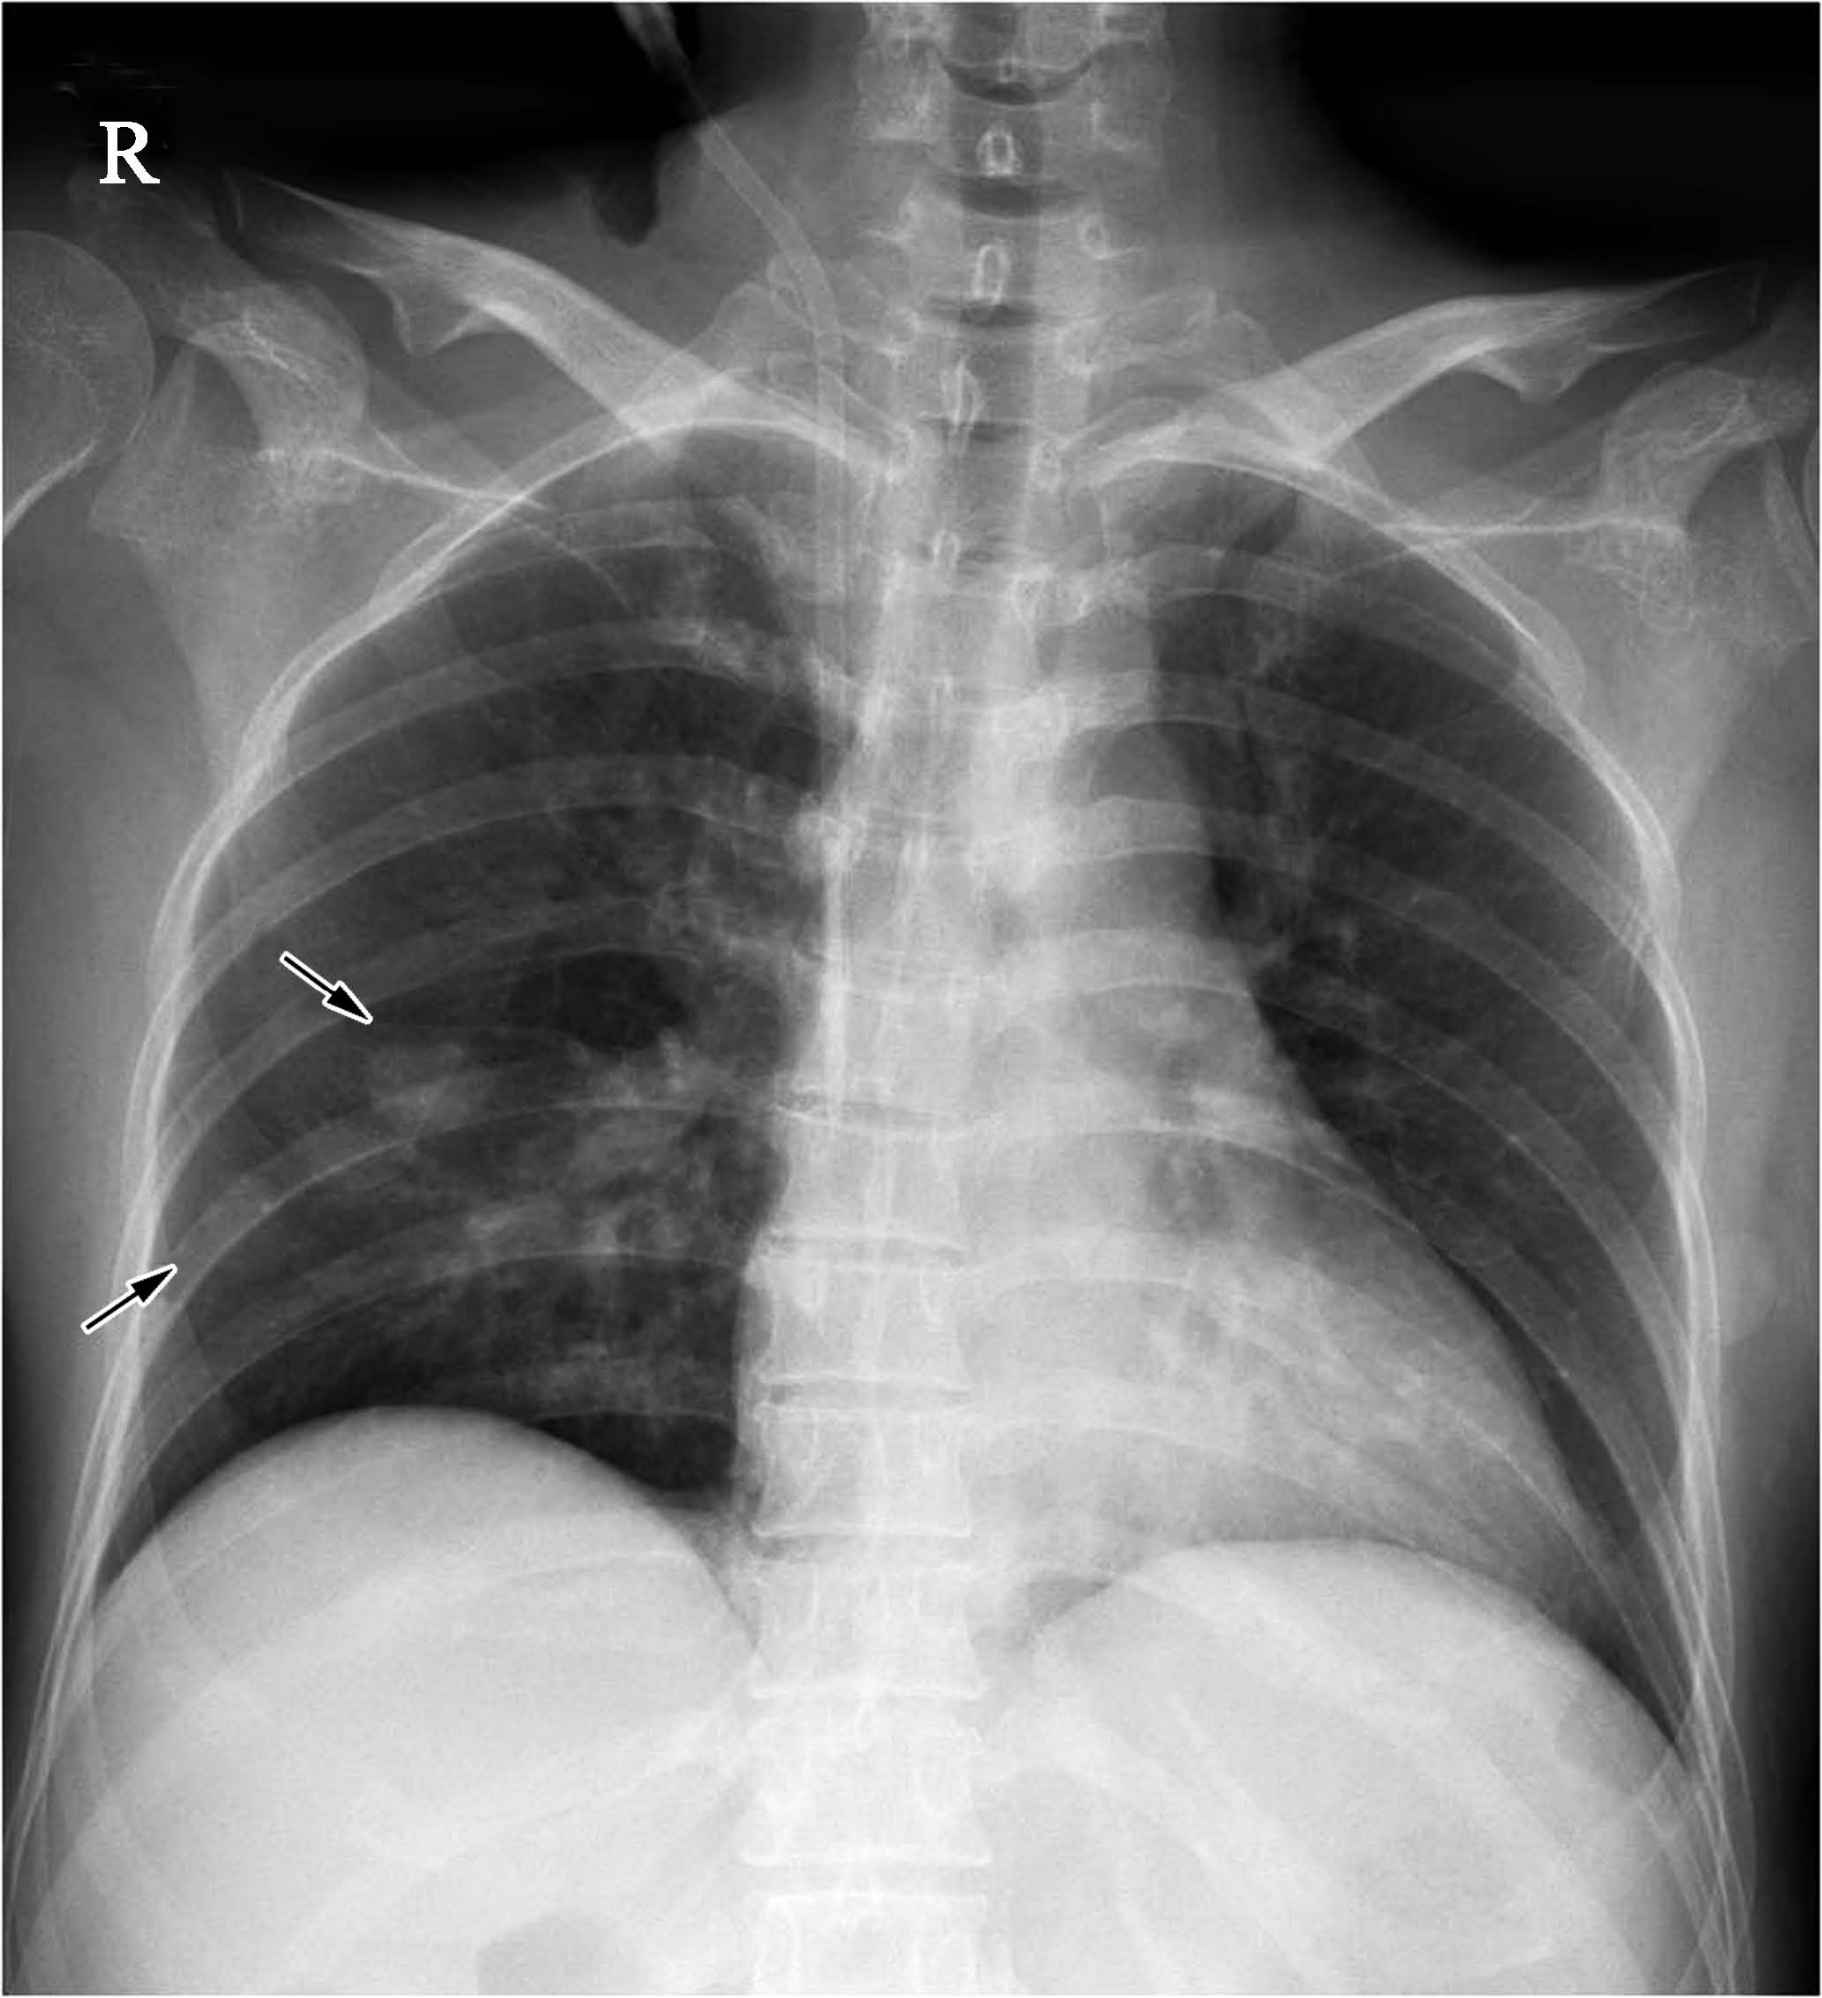
\includegraphics{./images/Image00161.jpg}
 \captionsetup{justification=centering}
 \caption{肺真菌病}
 \label{fig3-6-1}
  \end{figure} 

\textbf{【病史摘要】}  重症肝炎患者,伴咳嗽、胸痛和咯血3天。

\textbf{【X线表现】}
 右肺中下野内见多个类圆形结节影,边界清晰,密度尚均匀,右下肺纹理增粗。余肺野内未见明显异常密度影。心脏大小、形态未见明显异常。双侧肋膈角锐利。

\textbf{【X线诊断】}  右中下肺真菌(曲菌)感染可能大。

\textbf{【评  述】}
 肺真菌病临床并不少见。感染方式可分为两大类:一类为原发性感染,为吸入大量真菌孢子污染物所致;另一类为机遇性感染,患者常有严重感染、恶性肿瘤、血液病等全身疾病基础,自身免疫功能抑制,或长期使用糖皮质激素、化疗药物等使机体免疫功能进一步降低,长期大剂量抗生素应用抑制细菌的生长,故真菌病以继发感染为主。常见致病菌为曲菌、白色念珠菌、隐球菌等,较少见的有毛霉菌等。肺真菌感染多为吸入感染,少数经血行淋巴管路径。肺真菌感染的病理改变主要有过敏反应、炎性渗出、肉芽肿、出血、坏死及脓肿。除曲菌外,大多数肺真菌感染X线表现缺乏特征性。影像常表现为局限或广泛实变影,多发结节或肿块及空洞,机遇性真菌感染病变多弥漫分布。肺真菌病确诊依赖组织学检查。

肺曲霉菌病主要因吸入曲菌孢子而发病。曲菌在呼吸系统主要引起三种不同类型的病变:①曲菌球;②侵袭型;③过敏性支气管肺曲菌病。本病例结合重症肝炎病史,符合侵袭型曲菌病表现。血管侵入型肺曲菌病早期表现为单个或多个结节或肿块样实变。CT检查可见边缘模糊,周围伴磨砂玻璃样密度影(晕征),其病理基础为出血性肺梗死,结节或肿块为坏死肺组织,周围晕环为出血区,晚期进展为厚壁空洞性病变。另一特征性表现为新月征,圆形肺浸润伴有中心坏死和周围新月状或环形空洞,多出现于治疗后的恢复期。其他表现有多发小叶实变影或小叶融合性阴影、以胸膜为基底的多发楔形阴影或空洞。

\section{胸部寄生虫病}

\subsection{肺包虫囊肿}

\begin{figure}[!htbp]
 \centering
 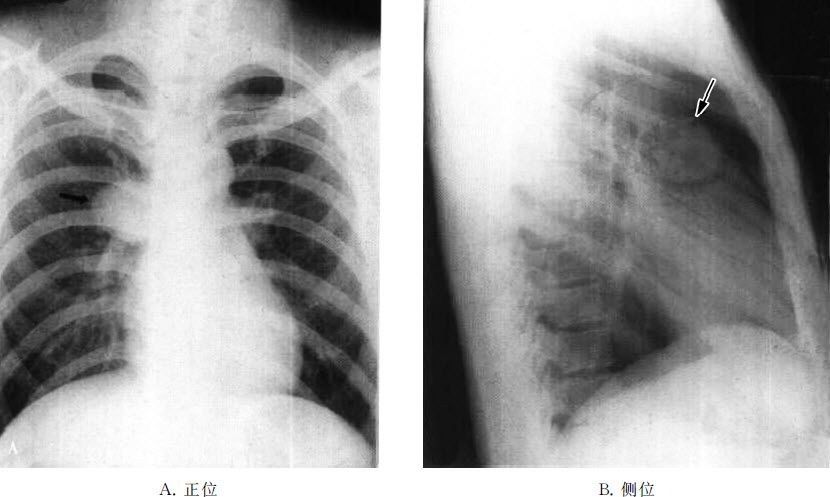
\includegraphics{./images/Image00162.jpg}
 \captionsetup{justification=centering}
 \caption{肺包虫囊肿}
 \label{fig3-7-1}
  \end{figure} 

\textbf{【病史摘要】}
 男性,32岁。疲劳,痰中带血3个月,胸透发现右上肺肿块约4cm。体格检查:无特殊。实验室检查:Casoni皮内试验呈阳性,血液中嗜酸性粒细胞比例升高。

\textbf{【X线表现】}
 气管居中。右肺上叶前段见一圆形块状阴影,约4cm大小,密度均匀,边缘光滑整齐。余肺野清晰,心影形态大小属正常。双侧肋膈角锐利。

\textbf{【X线诊断】}  结合患者生活史及临床表现,考虑右肺包虫囊肿。

\textbf{【评  述】}
 本病例经手术证实为肺包虫囊肿。肺包虫病多见于牧区,是由犬绦虫蚴寄生肺内所致。患者食入被犬绦虫卵污染的食物引起感染。患者一般无症状,感染时可有咳嗽、咳痰、咯血及胸痛。巨大囊肿引起呼吸困难,囊肿破裂可咯出囊壁碎片。囊肿感染可出现肺脓肿症状。X线表现为肺内肿块性病变,密度较淡而均匀一致,形态呈类圆形或卵圆形,边缘光滑。常位于两肺下野,以右肺下野多见。一般单发,有时于肿块顶部或外侧见到新月形空气间隙,又称肺半月征。囊肿若与支气管相通则形成气液平面,其上缘凹凸不平,漂浮许多小子囊,称水上浮萍征。巨大囊肿可压迫周围肺组织,陈旧性包虫囊肿壁可发生钙化。肺包虫病为囊性病变,X线影像为肺内球形病灶,边缘光滑,囊肿破裂后有典型X线影像表现,进一步CT增强检查,病灶无强化。患者有牧区居住和家禽接触史,20%的病例血液嗜酸性粒细胞比例增高。

Casoni皮肤试验和补体结合试验阳性有助于诊断,可为诊断依据。特别在流行区域生活过的患者,肺内发生球形阴影,要想到包虫囊肿的可能。

\section{肺肿瘤}

\subsection{中央型肺癌(一)}

\begin{figure}[!htbp]
 \centering
 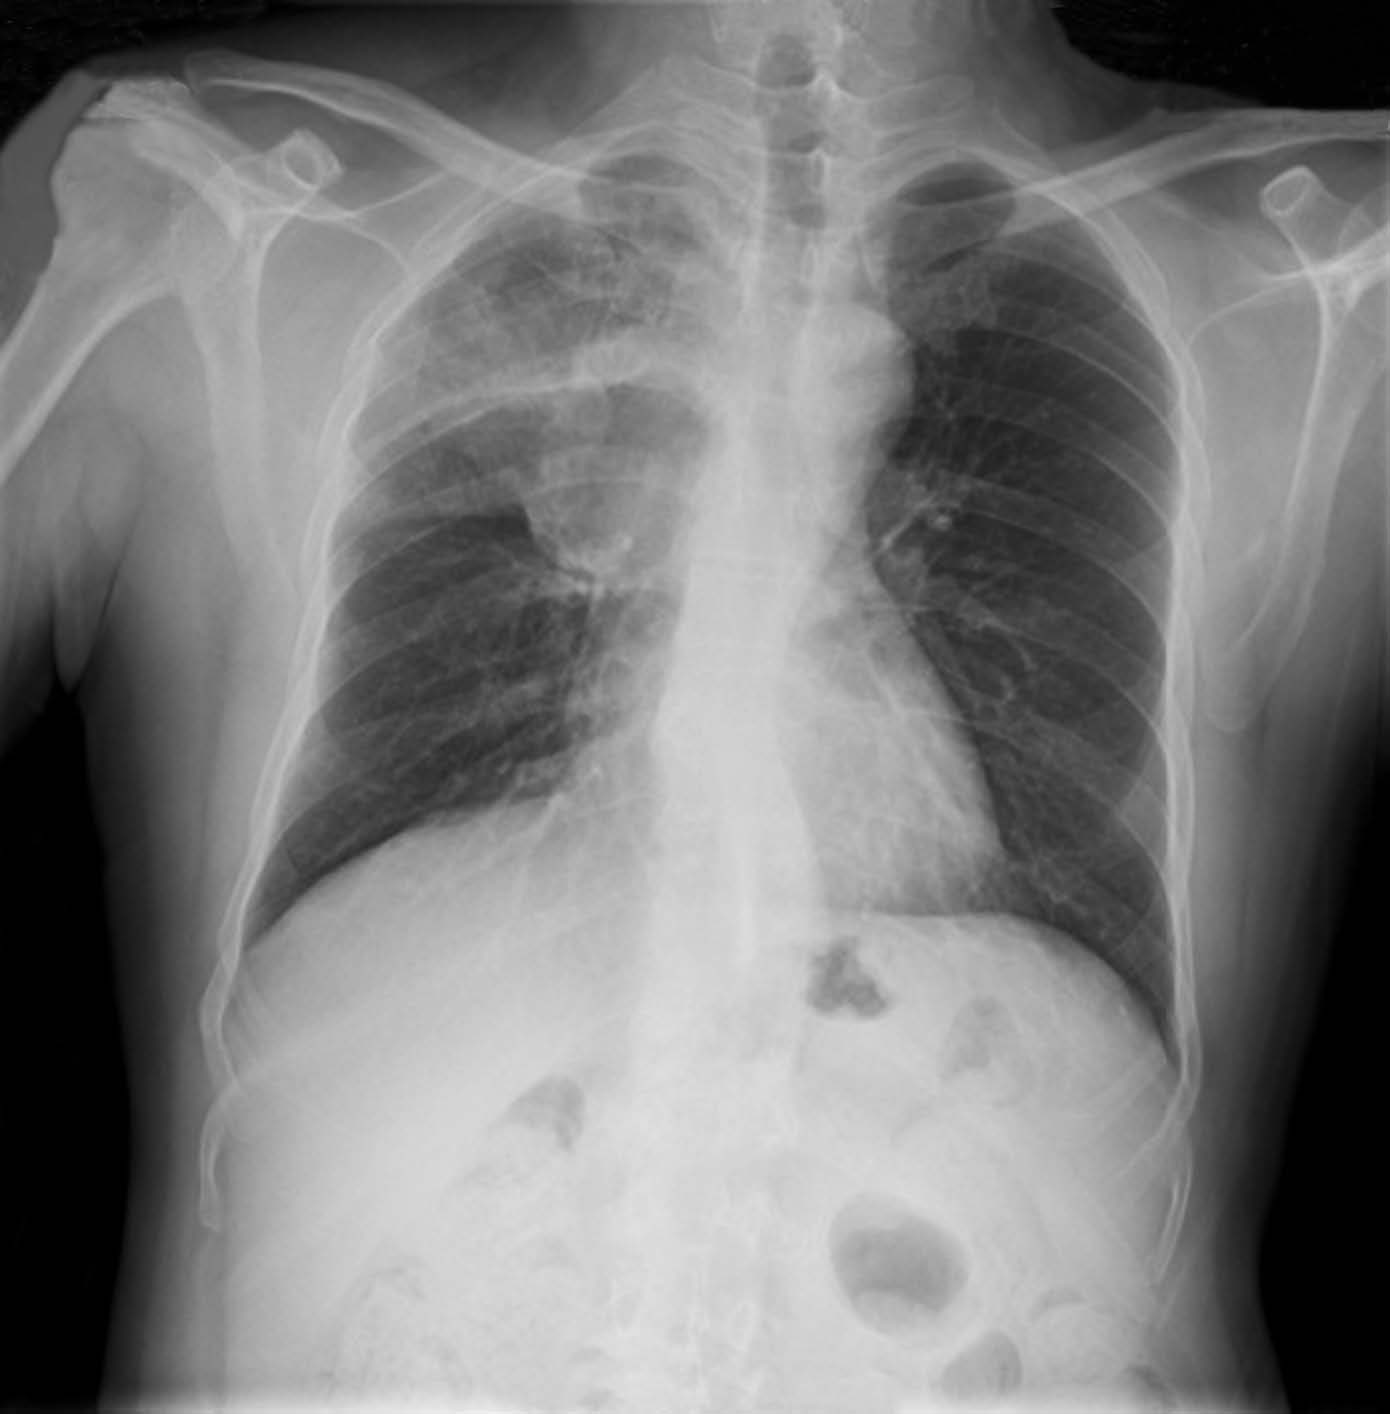
\includegraphics{./images/Image00163.jpg}
 \captionsetup{justification=centering}
 \caption{中央型肺癌(一)}
 \label{fig3-8-1}
  \end{figure} 

\textbf{【病史摘要】}
 男性,56岁。咳嗽、咳痰、胸痛伴咯血半年。体格检查:患者神志清,右上肺呼吸音降低,未闻及干湿啰音,心率75次/分,律齐。

\textbf{【X线表现】}
 气管向右侧移位。右肺上叶见大片状致密影,右侧水平裂上移,右肺门见类圆形肿块,构成横S征。左肺内未见明显异常密度影。心脏大小未见明显异常。右侧膈肌略上抬。双侧肋膈角锐利。

\textbf{【X线诊断】}
 右肺门占位伴右肺上叶不张,右侧中央型肺癌可能性大。

\textbf{【评  述】}
 本病由于早期局限在支气管壁内生长蔓延,X线表现常无异常征象。当癌肿逐步增大形成肿块,向支气管腔内突入或环绕支气管壁生长使支气管腔产生狭窄,可产生阻塞性气肿和阻塞性肺炎。当支气管腔严重狭窄或阻塞时即可发生肺不张。另一方面由于癌肿向支气管壁外发展,侵犯周围肺组织,可在肺门区形成肿块。肺门区肿块是中央型肺癌的直接X线征象。本病例具有右肺门增大、增浓,形成肿块伴右肺上叶不张等征象。增大的右肺门肿块下缘和不张且向上方移位的右肺上叶下缘构成典型的横S征。

在诊断中央型肺癌时,应注意以下几个问题:①正常肺门阴影大小差别很大,应注意两侧肺门大小的对比,更为重要的是仔细观察肺门的血管和支气管结构、密度和形态的改变,来判断有无肿块的存在,对可疑病例进一步行CT检查。②阻塞性肺炎的特点是往往经过抗生素治疗后吸收缓慢,吸收不完全,或在同一部位反复发生炎症,另外阻塞性肺炎往往伴有阻塞性肺不张。③结合临床,患者年龄较大,咳嗽、痰中带血丝,应考虑肺癌。

\subsection{中央型肺癌(二)}

\begin{figure}[!htbp]
 \centering
 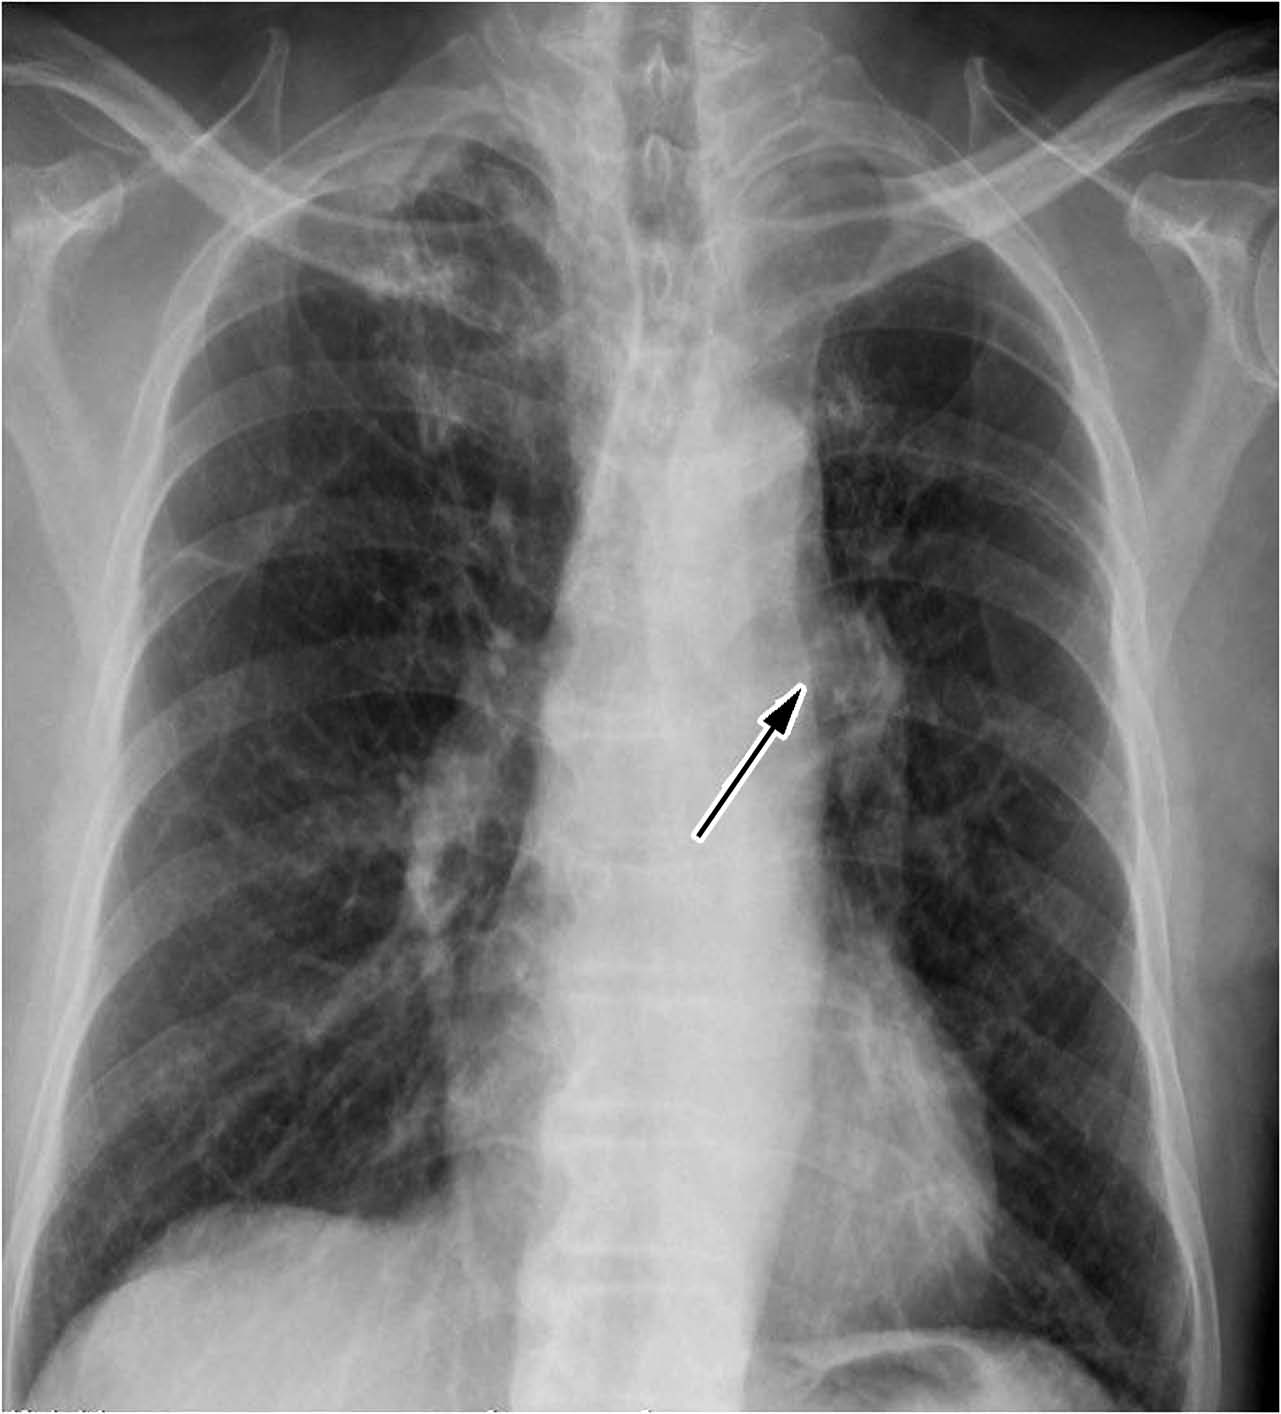
\includegraphics{./images/Image00164.jpg}
 \captionsetup{justification=centering}
 \caption{中央型肺癌(二)}
 \label{fig3-8-2}
  \end{figure} 

\textbf{【病史摘要】}
 男性,78岁。曾有“慢性支气管炎,肺气肿”病史20余年。主诉:痰中带血2周。吸烟史50年,每天20支。体格检查:双肺可见少许干湿啰音。

\textbf{【X线表现】}
 气管略向左侧扭曲。左侧肺门略增大、增浓。双侧肺纹理增多、增粗、紊乱。右肺尖见斑片状高密度致密影。心影形态大小属正常。双侧膈面略降低。

\textbf{【X线诊断】}
 ①左侧肺门增大、增浓-占位可能,建议增强CT检查。②右肺尖陈旧性病灶。③符合双肺慢性支气管炎,肺气肿改变。

\textbf{【评  述】}
 肺门肿块是进展期中央型肺癌的最常见、最直接X线及CT表现。管壁型及管外型均可在肺门部形成肿块阴影,鳞癌病变晚期及小细胞肺癌的肺门部肿块往往由肿瘤和转移性肿大淋巴结融合而成。虽然中央型肺癌在形成肺门肿块时,常伴有三阻征,但有时可仅出现肿块。此时,X线胸片有时需要仔细观察才可发现。胸部增强CT可很好地观察到肺门增大,运用增强后肺门血管和肿块间强化程度的差异和肺门支气管的通畅与否,判断是否存在肺门肿块。

\subsection{中央型肺癌(三)}

\begin{figure}[!htbp]
 \centering
 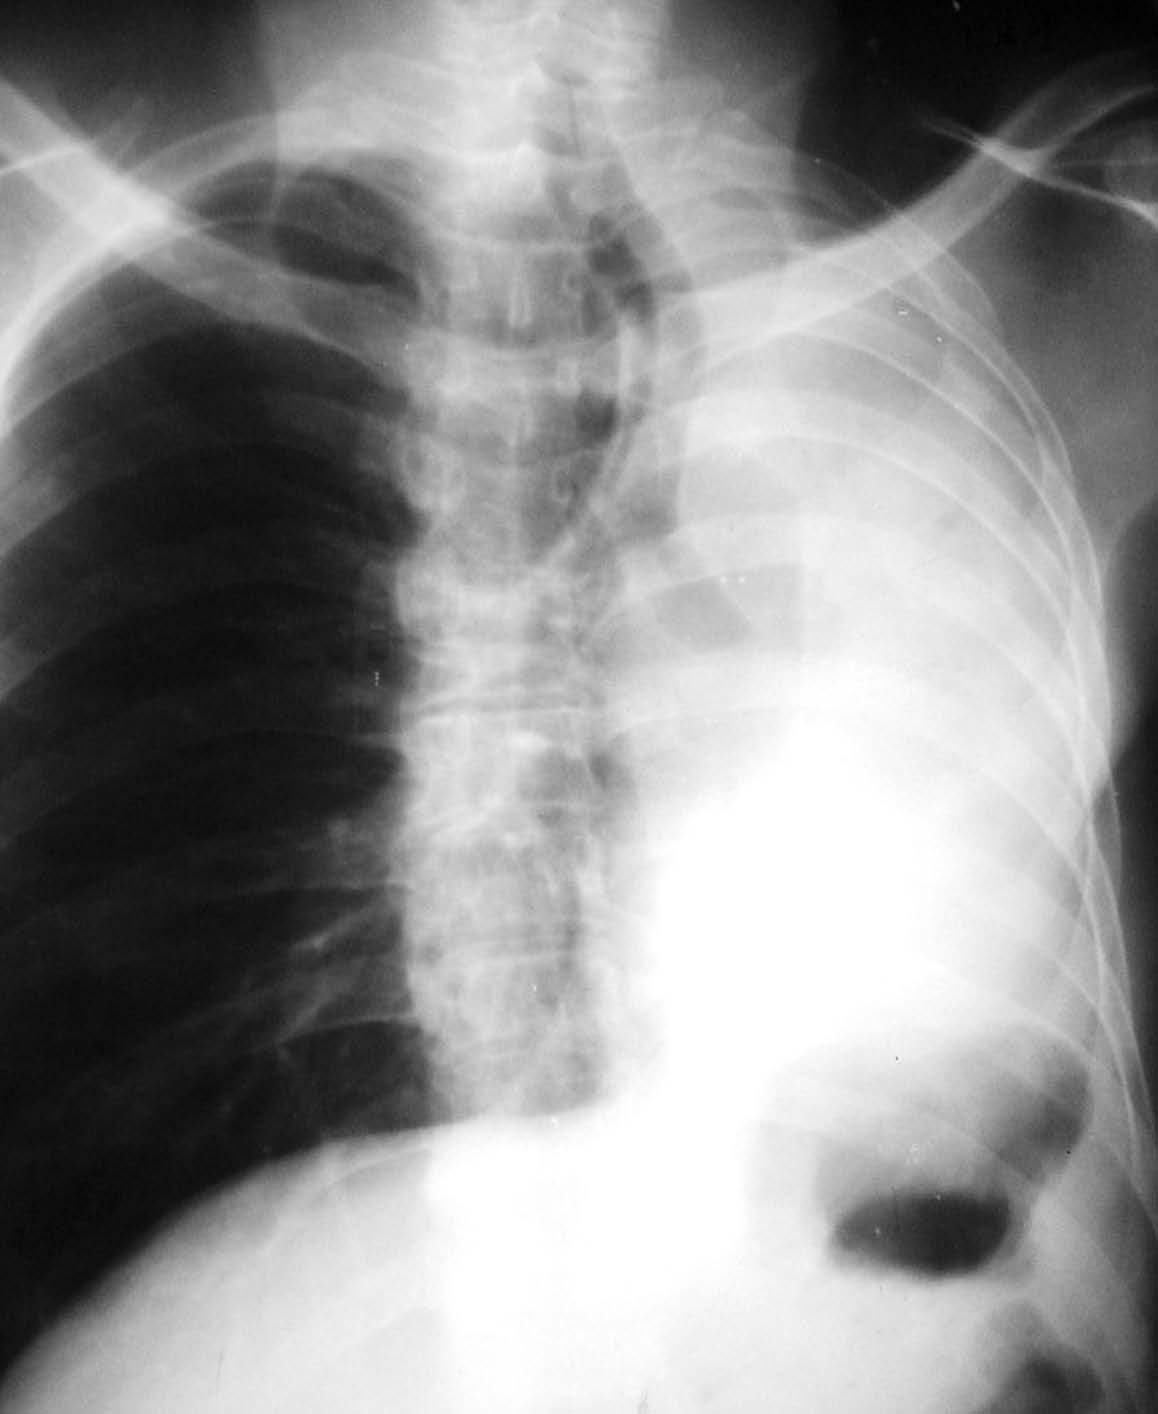
\includegraphics{./images/Image00165.jpg}
 \captionsetup{justification=centering}
 \caption{中央型肺癌(三)}
 \label{fig3-8-3}
  \end{figure} 

\textbf{【病史摘要】}
 男性,72岁。干咳伴痰中带血、胸闷胸痛3个月余。体格检查:左肺呼吸音运动减弱,语颤减低,叩诊实音,听诊左侧呼吸音消失。

\textbf{【X线表现】}
 双侧胸腔不对称,左侧缩小。左侧肋间隙变窄。气管向左侧移位。左侧主支气管截断,左侧胸腔内见大片状密度均匀的致密影。右侧肺野透亮度增高。纵隔心影向左侧移位。右侧膈肌下移,左侧膈面及肋膈角消失。

\textbf{【X线诊断】}
 左侧中央型肺癌可能性大,伴左全肺不张,继发右肺代偿性气肿。

\textbf{【评  述】}
 本病例经纤维支气管镜证实为左主支气管鳞癌。中央型肺癌引起全肺不张时,表现为一侧肺野大片均匀的致密影,常需要与一侧大量胸腔积液相鉴别。全肺不张时,因肺体积萎缩,表现为一侧肋间隙变窄,纵隔向患侧移位,膈肌上移。一侧大量胸腔积液时,因胸腔内替代效应,表现为一侧肋间隙变宽,纵隔向健侧移位,膈肌下降。两者不同的X线表现,可资鉴别。

\subsection{周围型肺癌(一)}

\begin{figure}[!htbp]
 \centering
 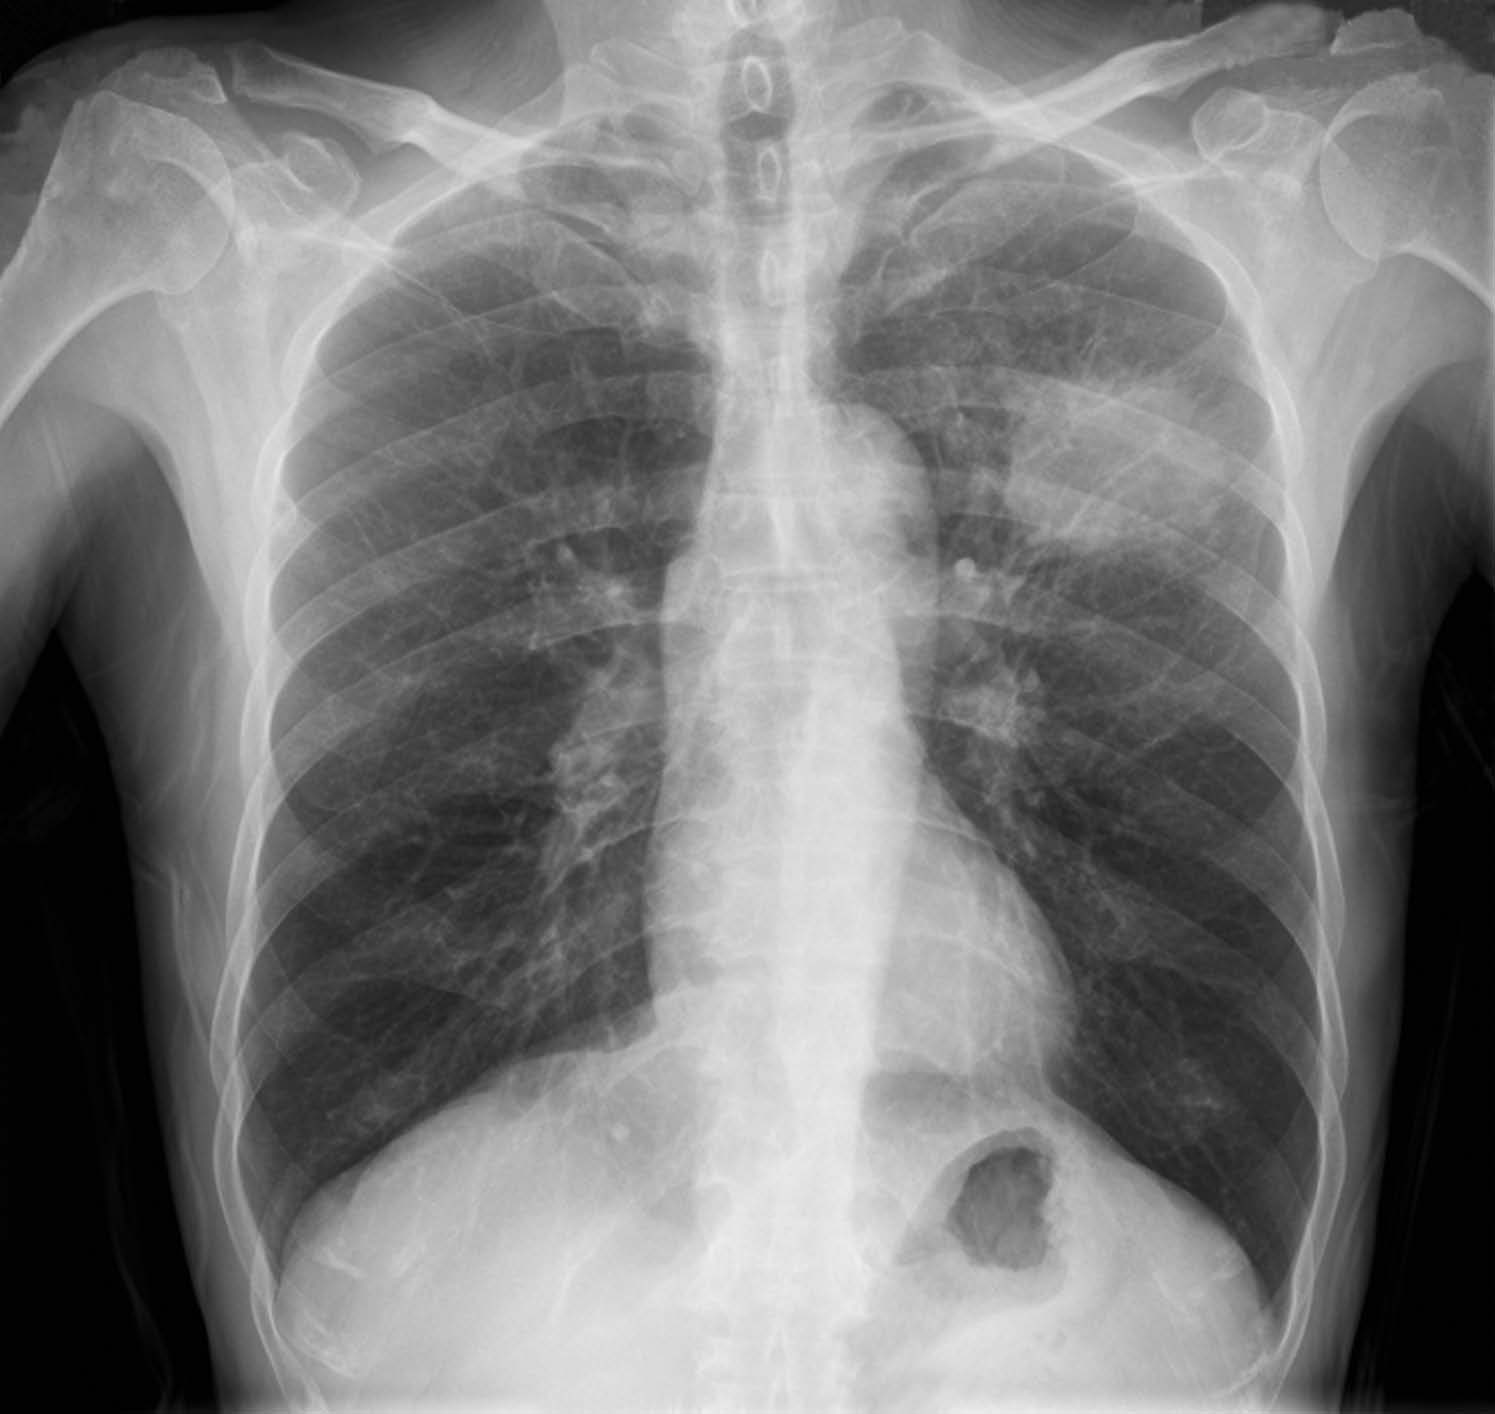
\includegraphics{./images/Image00166.jpg}
 \captionsetup{justification=centering}
 \caption{周围型肺癌(一)}
 \label{fig3-8-4}
  \end{figure} 

\textbf{【病史摘要】}
 男性,65岁。咳嗽、咳痰伴左胸痛3个月余,有时痰中带血丝。体格检查及实验室检查:无特殊改变。

\textbf{【X线表现】}
 气管居中。左肺中上野中带见一类圆形肿块影,直径约4.5cm,无明显分叶,边缘边界欠清晰,远端可见细微毛刺。余肺野内未见明显异常密度影。心脏形态、大小属正常。双侧肋膈角锐利。

\textbf{【X线诊断】}  左肺中上肺野占位,周围型肺癌可能性大。

\textbf{【评  述】}
 本病系指段及段支气管以远的肺癌。发生于段支气管者,由于支气管管腔较小,早期可致管腔狭窄发生肺段炎症或不张。发生于肺段支气管以远的肺癌主要形成局部肿块,肿块轮廓较清楚,常有分叶。周围型肺癌占肺癌的25%~42%。病变随着年龄增长有增多趋势。一般发病情况男多于女。按细胞类型区分鳞癌和未分化癌男性较多,腺癌女性较多。

周围型肺癌的症状与肿瘤的部位、类型、大小、病程阶段、有无并发症或转移等有关,包括咳嗽、咯血或血痰、胸痛、发热、消瘦和恶病质、副癌综合征、肺癌外侵和转移等。一般早期无症状,仅在体检时偶然发现。

周围型肺癌的球形阴影可为圆形、卵圆形或不定形的结节或肿块影。进行性增大,但生长速度绝非均匀一致。往往开始比较慢,但直径一旦达到2~3cm后,生长速度就显著增快,体积倍增时间平均在1~18个月。如果体积倍增时间<7天或>465天是实质性良性结节的表现。周围型肺癌可发生于肺内任何部位。结节/肿块的位置不能作为判断良、恶性的单独指标。

肺内球形阴影如大于3cm者多半为肺癌,如超过5cm而又有其他特殊表现,则肺癌可能性更大。实质性周围型肺癌一般为中等密度,比较均匀,但早期肺癌的密度大多数较淡,表现为纯磨玻璃或混合磨玻璃密度,X线胸片几乎不能检出。肿瘤边缘与肿瘤生长的情况相关。肿瘤生长时有时以膨胀性为主,有时以浸润性为主。前者表现为边缘整齐清楚,后者表现为边缘模糊不清。一般而言,肿块越大,边缘越清晰。边缘模糊不清者,常有细小毛刺状改变,有些平片就可以见到,大多数则需要行CT检查。肿瘤轮廓多有不同程度分叶现象。至于脐凹征、胸膜凹陷征等具有较高定性诊断价值,但往往需要行CT检查。

一般来说,肺癌发生钙化的概率远低于结核球。CT平扫可以发现更多的钙化,但肺癌钙化多为针尖状(弥漫)型或不定型,包埋邻近肉芽肿的钙化多见于癌肿的边缘。至于肺癌形成的空洞将在另一病例中评述。周围型肺癌可有邻近局部肺内转移,呈散在的小结节影。但最常见还是转移到肺门和(或)纵隔淋巴结。癌的淋巴结转移多数具有分叶状轮廓。周围型肺癌还可沿血管支气管束直接向肺门浸润,产生球形阴影与同侧肺门之间的条索状阴影,通常较细而紊乱,称癌性淋巴管炎。此时肺门通常已有肿大的淋巴结出现。

\subsection{周围型肺癌(二)}

\begin{figure}[!htbp]
 \centering
 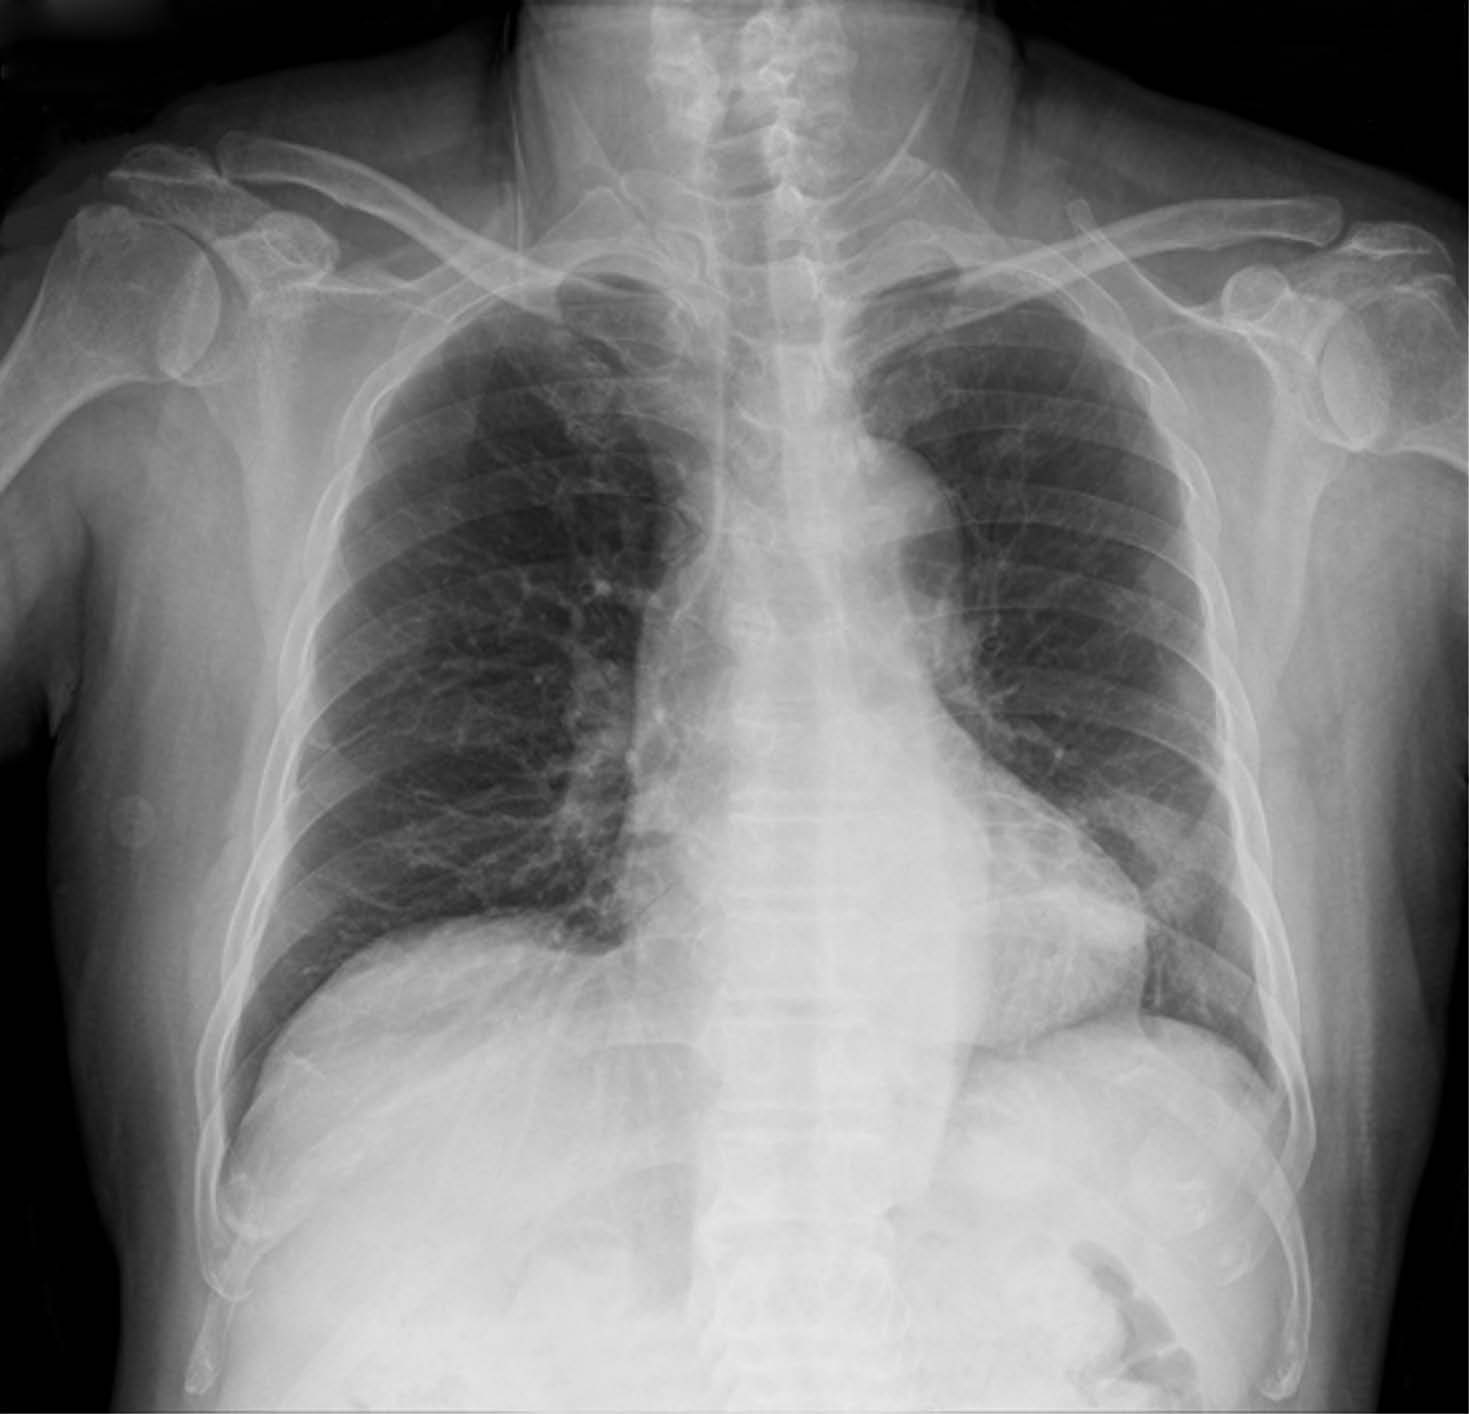
\includegraphics{./images/Image00167.jpg}
 \captionsetup{justification=centering}
 \caption{周围型肺癌(二)}
 \label{fig3-8-5}
  \end{figure} 

\textbf{【病史摘要】}
 男性,59岁。主诉:左侧胸痛2个月,伴咳痰。体格检查:无特殊。

\textbf{【X线表现】}
 气管居中。左肺下野中外带见一空洞性肿块影,直径约3.2cm,肿块轻度分叶,边缘模糊,洞壁厚,位于肿块中央,其内未见液平。余肺野内未见明显异常密度。心影略增大,心尖略向左侧扩大。主动脉轻度迂曲增宽。左侧肋膈角稍钝,右侧锐利。

\textbf{【X线诊断】}
 左肺下野厚壁空洞性占位,周围型肺癌形成空洞可能性大。心脏增大,左侧胸膜增厚。

\textbf{【评  述】}
 空洞为瘤内圆形或类圆形空气样透亮影。超过15%的肺癌可见空洞形成,大多直径>3cm,但也可见于直径仅7mm的小肺癌。有研究统计100例周围型小肺癌内的空洞发生率为4%。按组织类型统计,鳞癌空洞发生的机会较其他类型肺癌高得多,其次是腺癌。癌性空洞典型的X线表现为厚壁或壁厚不均,个别病例壁菲薄,内壁凹凸不平,并可见壁结节;外壁多见分叶及毛刺;多数为中心性,少数为偏心性;大小不一(1~10cm),壁厚不等(0.5~3cm)。当结节的不规则空洞壁厚度>16mm时,恶性可能性大(84%~95%的孤立性肺结节);而良性病变多为薄壁光滑性空洞,当洞壁<4mm时,95%的结节为良性。但是因为良、恶性空洞特征的广泛重叠性,仅仅依靠空洞壁的厚度、光滑与否、有无壁结节有时难以鉴别病变的良、恶性,尤其是≤3cm的小肺癌。更重要的是观察病灶基本形态学特征:结节和(或)肿块的分叶、脐凹、毛刺及典型胸膜凹陷征等恶性可能大,而急性肺脓疡空洞则多见邻近肺组织内炎性渗出性改变,结核性空洞多见卫星灶及肺内其他部分播散灶。

\subsection{肺上沟癌}

\begin{figure}[!htbp]
 \centering
 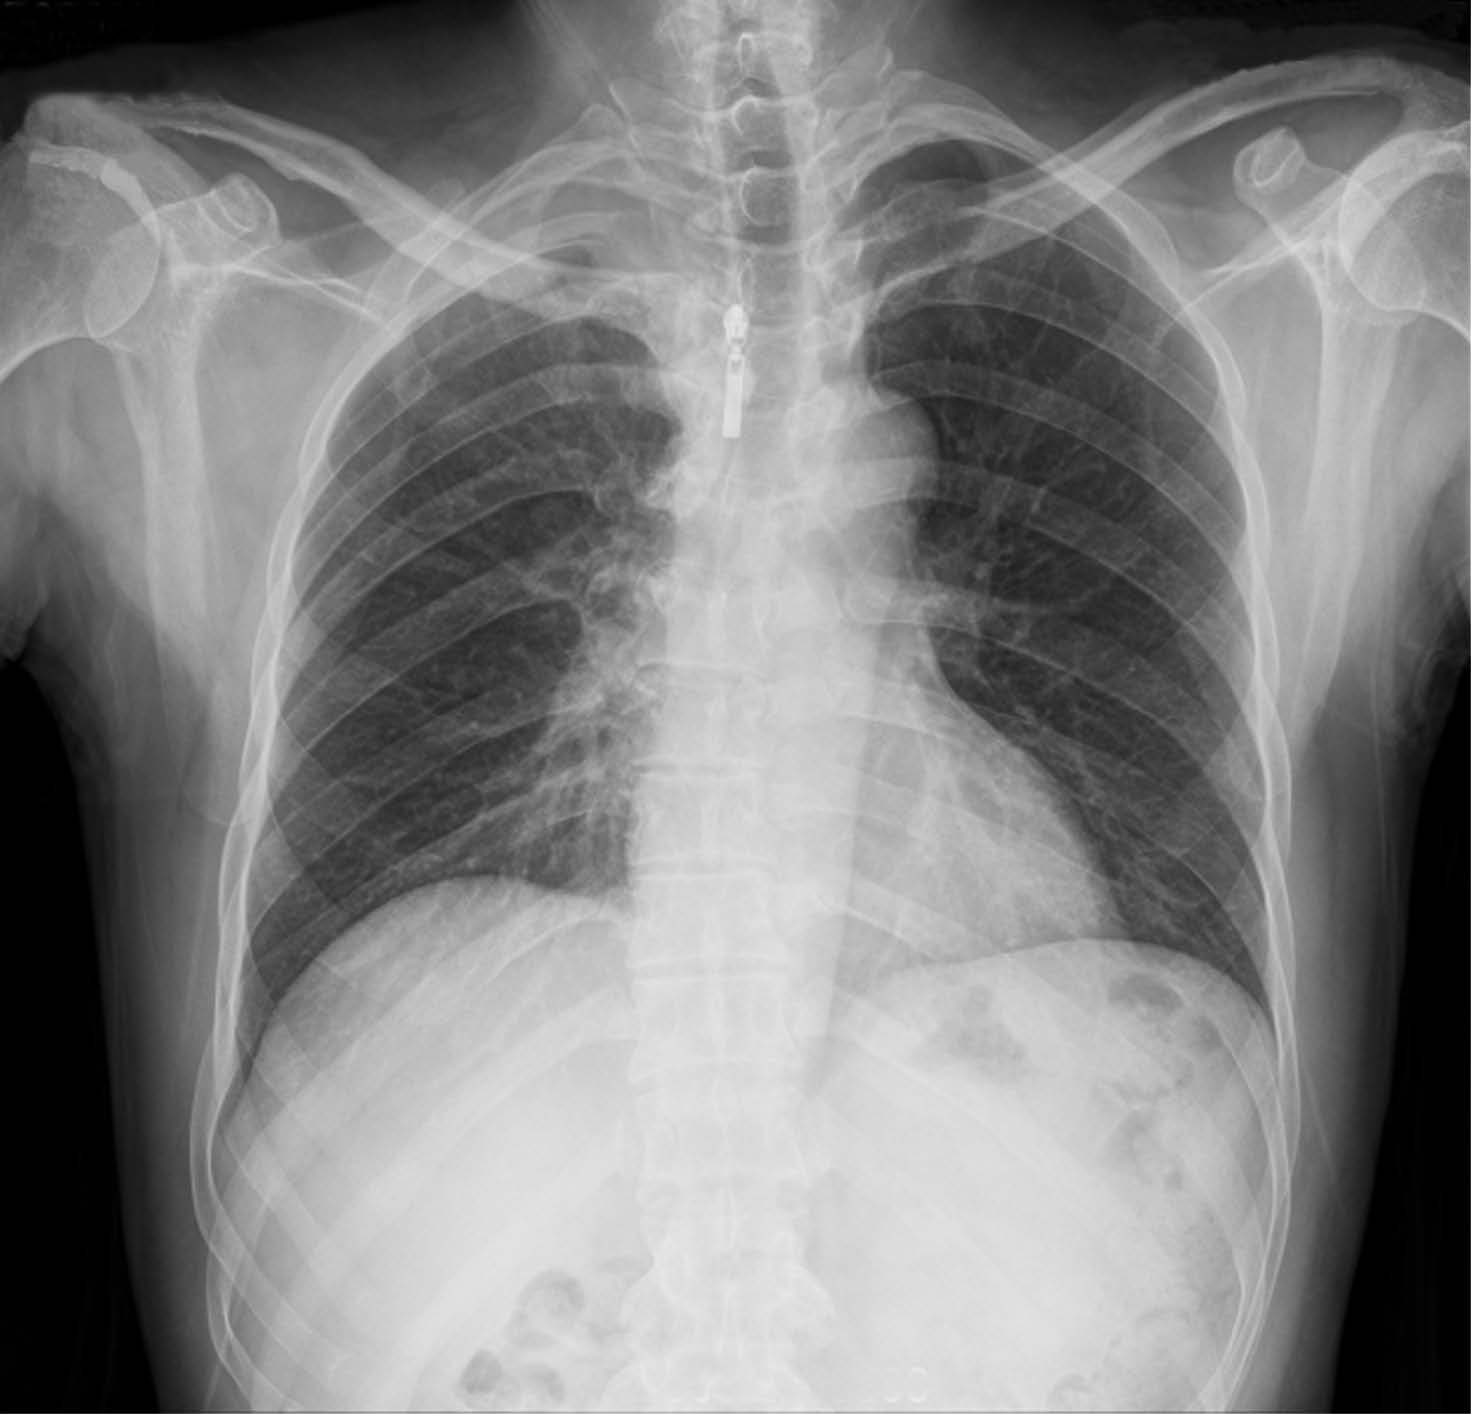
\includegraphics{./images/Image00168.jpg}
 \captionsetup{justification=centering}
 \caption{肺上沟癌}
 \label{fig3-8-6}
  \end{figure} 

\textbf{【病史摘要】}
 男性,51岁。右肩部疼痛,并放射至右侧上肢,不能上举2个月余。余无特殊。

\textbf{【X线表现】}
 双侧胸廓不对称,右侧上部肋间隙变窄,右肺尖见片状均匀性致密影,其内缘及下缘隆起。双侧肺纹理增多、增粗。心脏形态、大小属正常。双侧肋膈角锐利。

\textbf{【X线诊断】}  右侧肺上沟癌可能性大。

\textbf{【评  述】}
 本病少见,仅占全部肺癌的1%,是指发生在肺上沟(指锁骨下动脉通过胸膜对肺上叶尖部的压迹)内的肺上沟癌(肺尖癌),由美国放射学家Pancoast于1924年首先描述。肺上沟癌主要表现为Pancoast综合征,通常侵犯第2或第3肋骨、锁骨下血管、臂丛、星状神经节及邻近的胸椎椎体。Pancoast综合征的特征性表现是疼痛,发生在肩部、胸壁或放射至颈部。Horner综合征因肺上沟癌压迫或侵犯椎体旁交感神经链引起,出现同侧瞳孔缩小,上眼睑下垂,额部少汗等体征。C8、T1神经根受侵犯时,表现为尺神经分布区疼痛、无力或麻痹。肺上沟癌,组织病理学以肺鳞癌最多见,其次是肺腺癌及大细胞癌。影像学检查可见肺尖部软组织密度肿块,并可见肿瘤侵犯胸壁,破坏肋骨、胸椎及颈椎等结构,但以CT、MRI较X线显示清晰。薄层CT冠状位图像重组或冠状位MRI有助于鉴别肺上沟癌并判断肿瘤确切侵犯范围。

\subsection{弥漫型细支气管肺泡癌(一)}

\begin{figure}[!htbp]
 \centering
 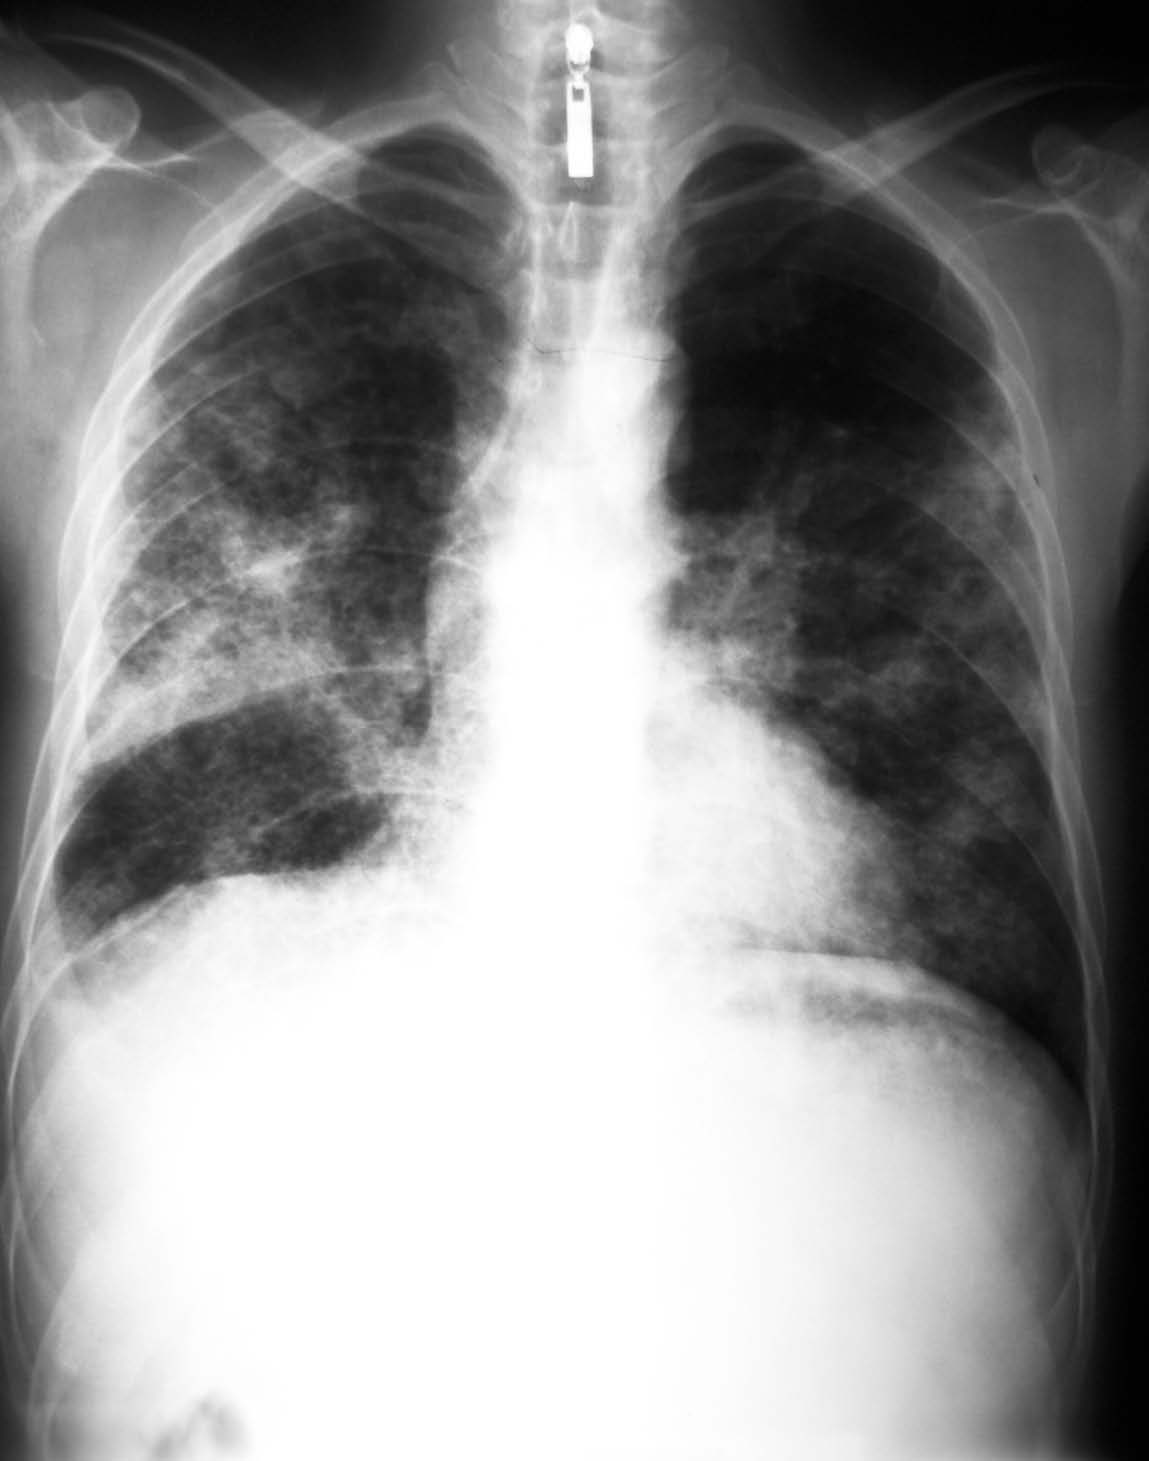
\includegraphics{./images/Image00169.jpg}
 \captionsetup{justification=centering}
 \caption{弥漫型细支气管肺泡癌(一)}
 \label{fig3-8-7}
  \end{figure} 

\textbf{【病史摘要】}
 男性,48岁。咳嗽、咳痰2年,加重伴喘憋3个月入院,体温36.8℃。体格检查:一般情况较差,消瘦,呼吸急促,双肺可闻及哮鸣音,心脏听诊无杂音。患病以来,体重下降5kg。曾行支气管镜及肺泡灌洗,管腔内未见阻塞与狭窄,病理提示:少量纤维柱状上皮,下方有纤维组织增生,少量的小血管及淋巴细胞浸润。

\textbf{【X线表现】}
 气管居中。双侧肺纹理增粗。双肺野内见弥漫性分布、边界不清、密度不均匀的片状及大片状致密阴影及结节阴影。左侧肺门影增大。心脏形态大小属正常。左侧肋膈角锐利,右侧变钝。

\textbf{【X线诊断】}
 结合临床,首先考虑弥漫型细支气管肺泡癌伴左侧肺门淋巴结肿大及右侧胸腔中等量积液。

\textbf{【评  述】}
 本病X线及CT表现为双肺多发结节或弥漫型肺段/肺叶实变。弥漫型细支气管肺泡癌病例占细支气管肺泡癌的50%左右。本病例属于弥漫型肺段/叶实变伴结节。结节和实变均为肿瘤细胞在肺泡表面生长扩散而无肺泡间隔的破坏(伏壁式生长);磨砂玻璃密度影还可反映肺泡腔内大量低密度粘液或肿瘤细胞的肺泡壁伏壁式生长而肺泡腔未完全充填;一个肺段/肺叶实变是肺泡腔内粘液进展至整个肺段/肺叶的结果,也反映了细支气管肺泡癌粘液型的亚型。弥漫型细支气管肺泡癌的患者病程往往发展较快,表现为进行性呼吸困难。临床表现不同,患者症状轻重不同,病程长短不一,可有发热、干咳、咳泡沫痰或血丝痰、胸闷等,预后较差。细支气管肺泡癌X线表现多种多样,可见肺实变影、磨砂玻璃密度影和多发结节影,但多以这两种征象中的某一种为主,三种征象混合存在为特征。高分辨率CT是最佳检查技术。病变在两肺的分布往往不对称,部分病变有融合倾向,形成大片实变(又称肺炎型肺癌)。尽管弥漫型细支气管肺泡癌的影像学表现多样,但当高分辨率CT上出现肺段/肺片实变、小叶中心性结节、磨砂玻璃密度影共存,伴肺门及纵隔淋巴结转移及胸腔积液时,则高度提示弥漫型细支气管肺泡癌。

\subsection{弥漫型细支气管肺泡癌(二)}

\begin{figure}[!htbp]
 \centering
 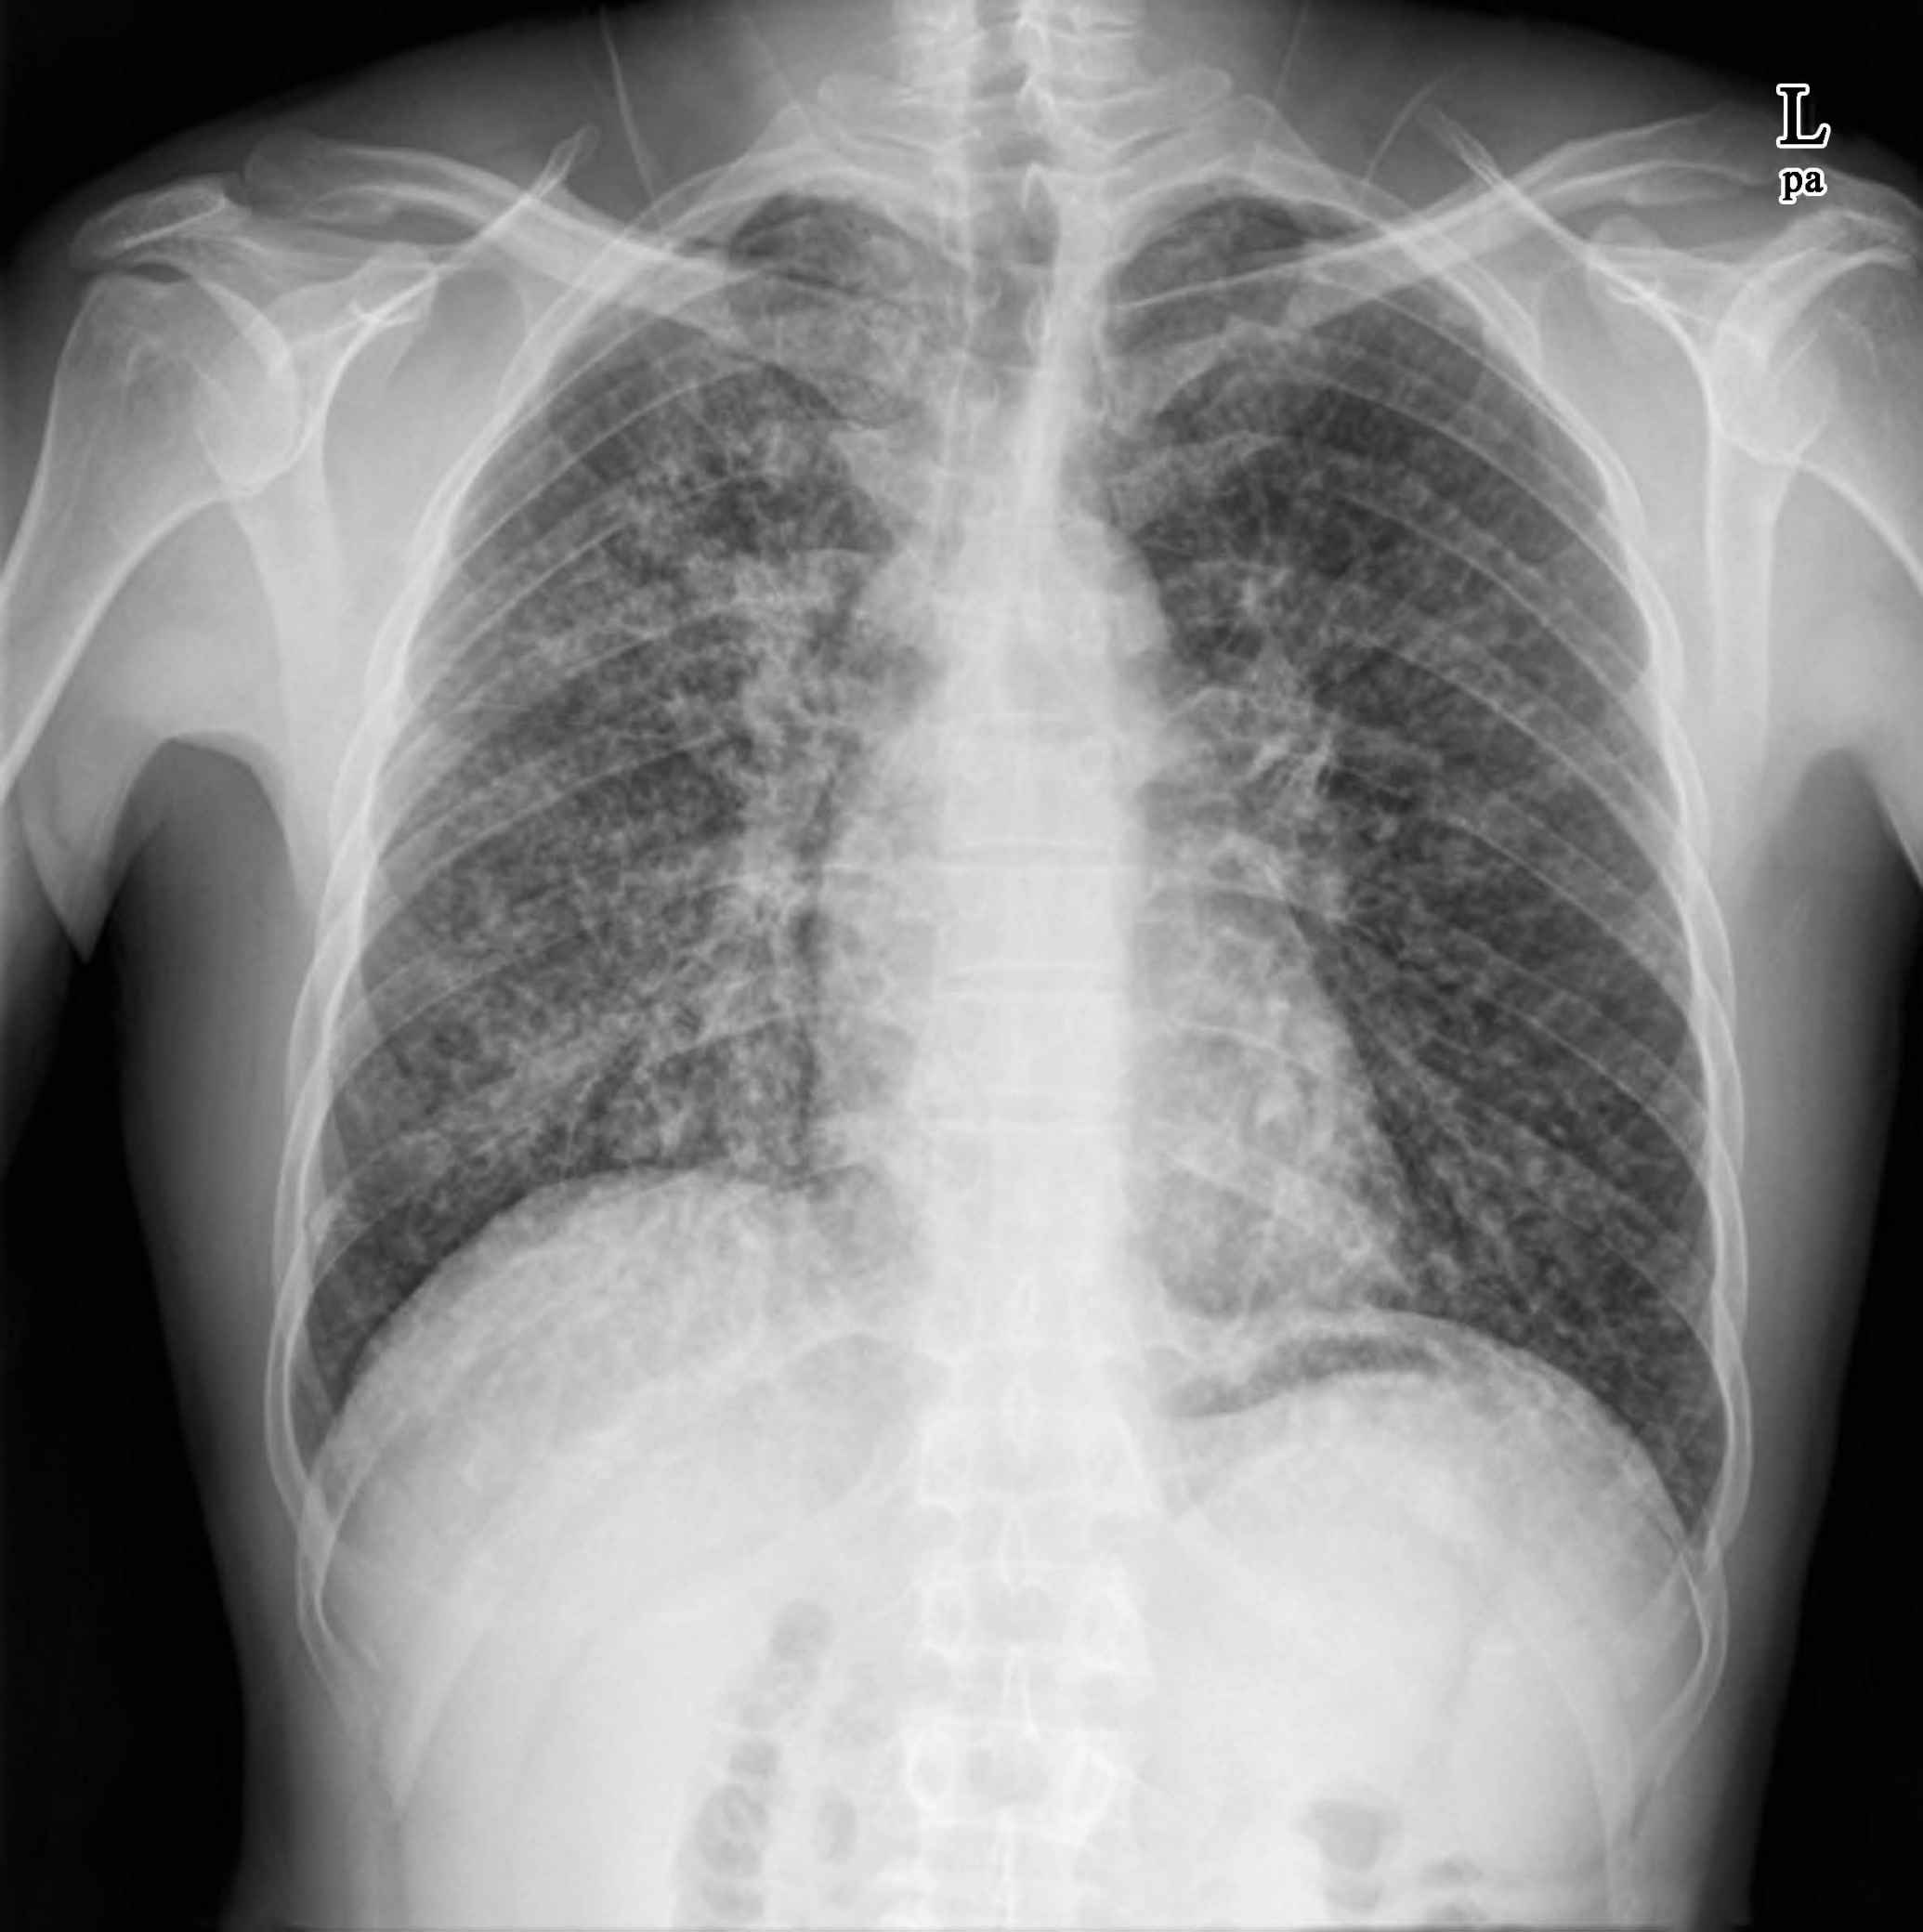
\includegraphics{./images/Image00170.jpg}
 \captionsetup{justification=centering}
 \caption{弥漫型细支气管肺泡癌(二)}
 \label{fig3-8-8}
  \end{figure} 

\textbf{【病史摘要】}
 男性,50岁。干咳、胸闷2个月,低热1周,经治疗后症状无明显改善。

\textbf{【X线表现】}
 气管居中。双肺纹理增多、增粗,伴弥漫型小结节影,小结节分布均匀,大小略不等。双下肺胸膜下见小叶间隔结节状增厚。左侧肺门可疑增大。心脏形态大小正常。双侧肋膈角锐利。

\textbf{【X线诊断】}
 双肺弥漫型结节伴小叶间隔增厚,弥漫型细支气管肺泡癌可能性大,转移性肺癌、粟粒性肺结核待排。

\textbf{【评  述】}
 本例经支气管镜检查,确诊为弥漫型细支气管肺泡癌。细支气管肺泡癌多发结节边界清晰或不清,大小可不一,小者犹如粟粒性肺结核,类似于肺外肿瘤肺转移,结节内可形成空洞,易发生淋巴道转移。多发结节型弥漫型肺泡细胞癌应与其他多发结节性病变如尘肺、结节病、血行播散型肺结核、肺转移瘤、过敏性肺泡炎相鉴别。

\subsection{隐匿型肺癌}

\begin{figure}[!htbp]
 \centering
 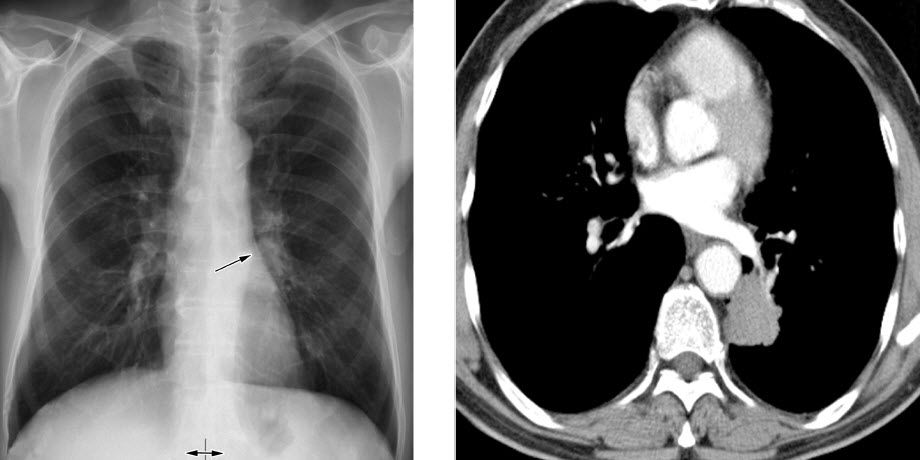
\includegraphics{./images/Image00171.jpg}
 \captionsetup{justification=centering}
 \caption{胸部X线正位和CT增强断层扫描}
 \label{fig3-8-9}
  \end{figure} 

\textbf{【病史摘要】}  男性,72岁。咳嗽,痰血10余天。

\textbf{【X线表现】}
 双侧胸廓对称。双肺纹理增多增粗。右上肺及右肺门处见点状钙化,心脏大小属正常。双侧肋膈角锐利。

\textbf{【X线诊断】}  右肺上叶陈旧性病变伴右肺门钙化淋巴结。

\textbf{【评  述】}
 常规X线和CT是诊断肺癌的重要手段。临床上我们把隐蔽在肺尖、肺门区、支气管内、奇静脉食管窝、脊椎旁、心影后、膈肌后、膈肌上、胸膜缘及胸水遮盖等区域的肺癌统称隐匿型肺癌,常规胸片不易检出、不易确诊,常需要借助CT检查才能得出正确结果。本病例X线正位胸片漏诊左肺门下方结节(箭头),CT增强检查示左肺下叶背段周围型肺癌,病理检查示鳞癌。侧位胸片或高千伏摄影有助于检出隐匿型肺癌。DR/CR摄影可通过调节图像亮度及对比度更清晰显示病灶与周围结构间密度对比,亦有助于诊断。隐匿型肺癌尚需与神经源性肿瘤、胸腺瘤、纵隔胸膜包裹性积液、胸膜肿瘤等鉴别。

\subsection{肺原发淋巴瘤}

\begin{figure}[!htbp]
 \centering
 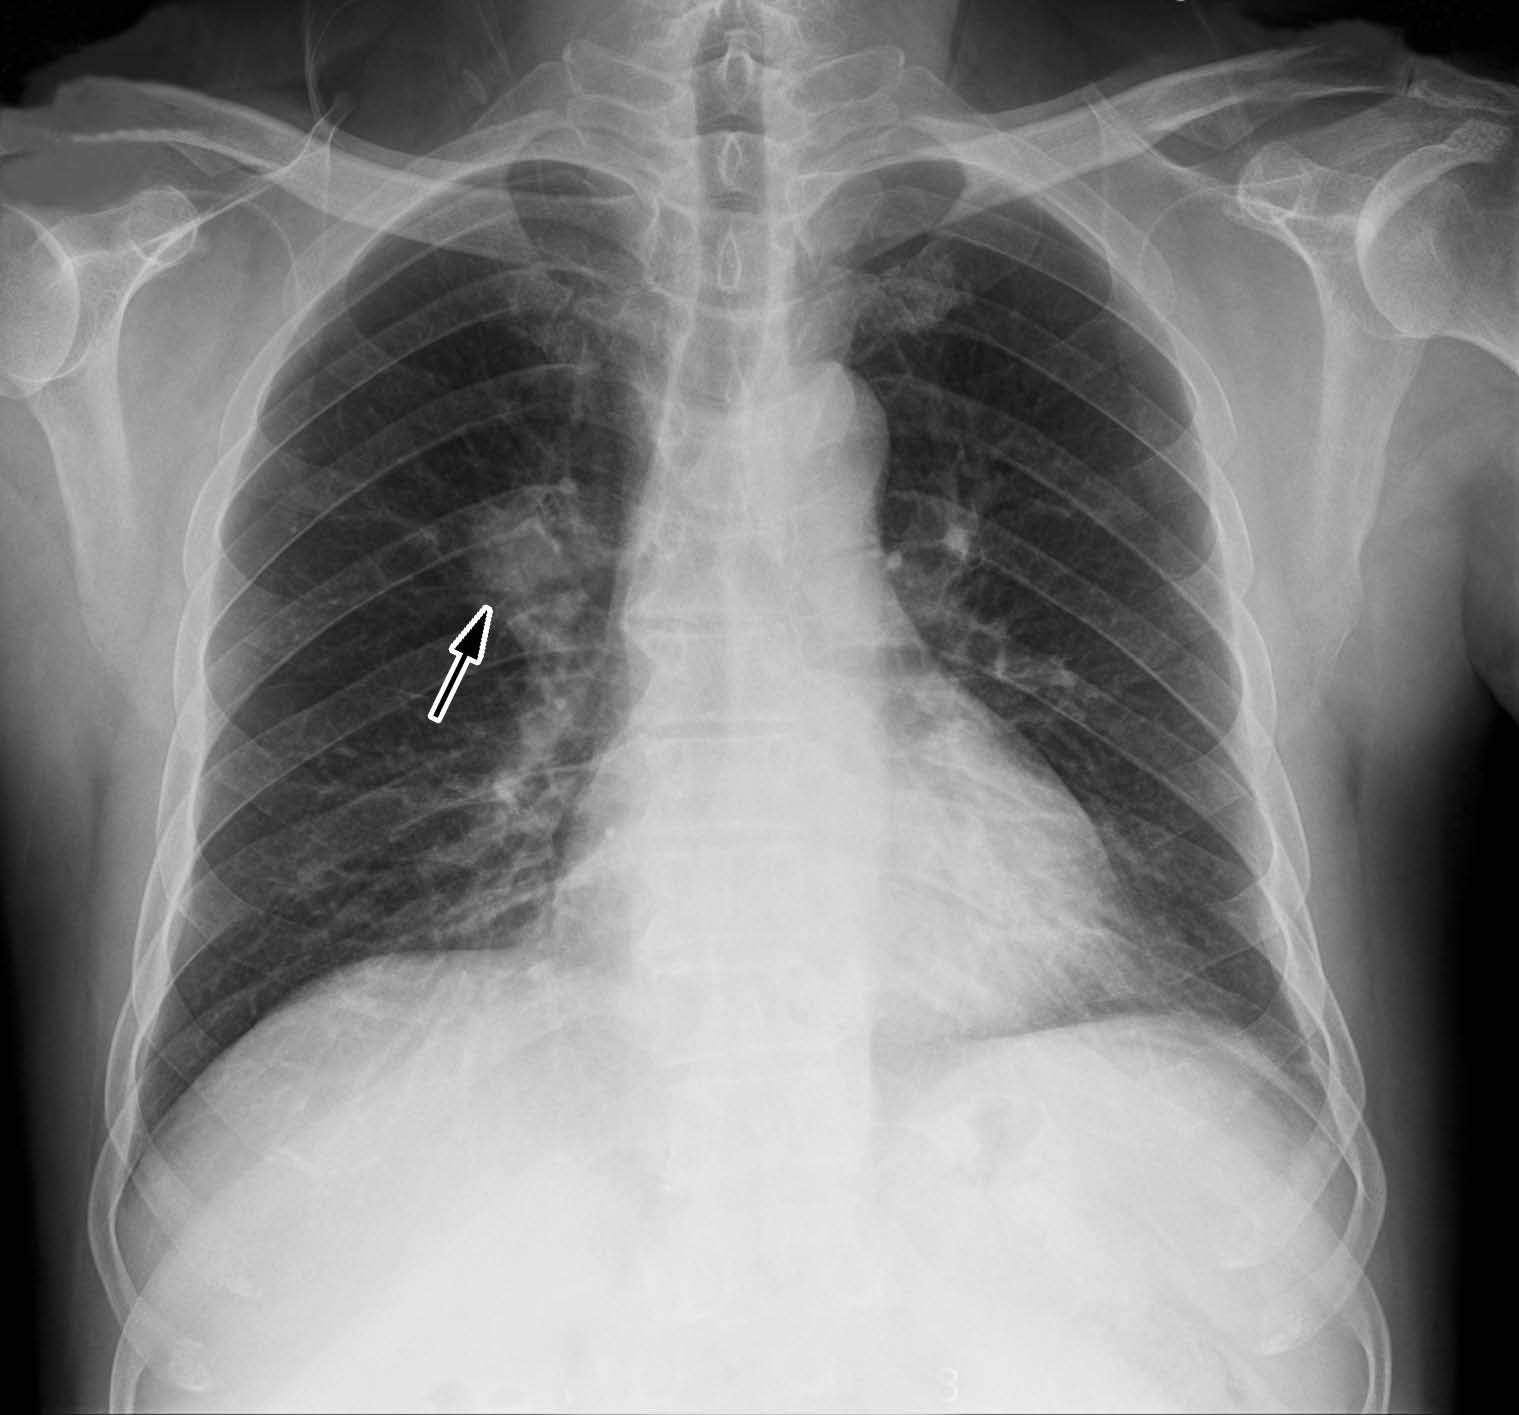
\includegraphics{./images/Image00172.jpg}
 \captionsetup{justification=centering}
 \caption{肺原发淋巴瘤}
 \label{fig3-8-10}
  \end{figure} 

\textbf{【病史摘要】}
 男性,60岁。因干咳2个月而来院就诊。体格检查:无特殊。

\textbf{【X线表现】}
 气管无移位。右肺门见一肿块影,直径约3.5cm,密度均匀,边缘稍模糊。肿块下方见充气支气管征,支气管无明显狭窄或扩张(箭头)。余肺野内未见明显异常密度影。心脏大小、形态属正常。双侧肋膈角锐利。

\textbf{【X线诊断】}  右肺门占位-中央型肺癌可能性大。

\textbf{【评  述】}
 本病例经手术切除后,确认为肺粘膜相关性淋巴瘤。肺原发性淋巴瘤定义为克隆性淋巴样增殖,影响单侧或双侧肺的实质和(或)支气管,且在诊断时及诊断后3个月内未发现肺外累及的证据。肺原发性淋巴瘤非常罕见,仅占结外淋巴瘤的3%~4%,占肺原发性恶性肿瘤的0.5%~1%。肺原发性淋巴瘤包括最常见的非霍杰金淋巴瘤(non-Hodgkin's
lymphoma,NHL)及少见的淋巴瘤样肉芽肿病。B细胞NHL占肺原发性淋巴瘤的58%~87%,90%以上为粘膜相关性非霍杰金淋巴瘤(mucosa-associated
lymphoid tissue
NHL,MALT-NHL)。肺原发性淋巴瘤起源于肺内淋巴组织,其中绝大部分为NHL,58%~87%为低度恶性-B细胞NHL,其中超过90%为MALT-NHL。MALT是一种仅存在于“粘膜屏障”中的淋巴组织。多数学者认为人的支气管粘膜正常情况下与胃粘膜有相似之处,通常不存在MALT,但由于各种抗原的刺激如吸烟、感染及自身免疫性疾病等的影响,使肺支气管粘膜形成获得性MALT,在此基础上可发生获得性MALT-NHL。

近半数的肺原发性淋巴瘤患者在诊断时无症状,大多是因肺部X线或CT检查异常而偶然发现。当出现症状时,无特异性,包括咳嗽、胸痛、轻度呼吸困难,偶尔出现咯血。

肺原发性MALT-NHL常见的影像学表现是双侧或单侧肺内的肿块、肿块样实变、多发结节,少数表现为双肺弥漫型浸润。MALT-NHL以一个或一个以上的肿块或肿块样实变最常见,其次是肺结节;两个以上的肿块、结节或实变见于大多数患者,孤立性病变见于少数患者。也有报道最多见的胸片表现为孤立性局限性病变;其次是两个以上的多发病灶。肺内结节的分布可在支气管血管束周围,也可在胸膜下区域,还可以是随机性分布。最多见的伴随征象是肿块、肿块样实变及结节内的充气支气管征,病灶内的气道约有一半伴有扩张,有些甚至可表现为空洞样。MALT-NHL累及到肺门纵隔淋巴结相对少见。

肺淋巴瘤的影像学表现多样,诊断困难。肺内多发病变,需考虑肺淋巴瘤的可能,病灶内充气支气管征及CT增强后肿块呈中等均匀强化是相对特异性征象,但须与肺炎、肺结核、肺癌及肉芽肿病变相鉴别,明确诊断需要行支气管镜穿刺活检、经皮穿刺活检或手术切除病理检查证实。

\subsection{错构瘤}

\begin{figure}[!htbp]
 \centering
 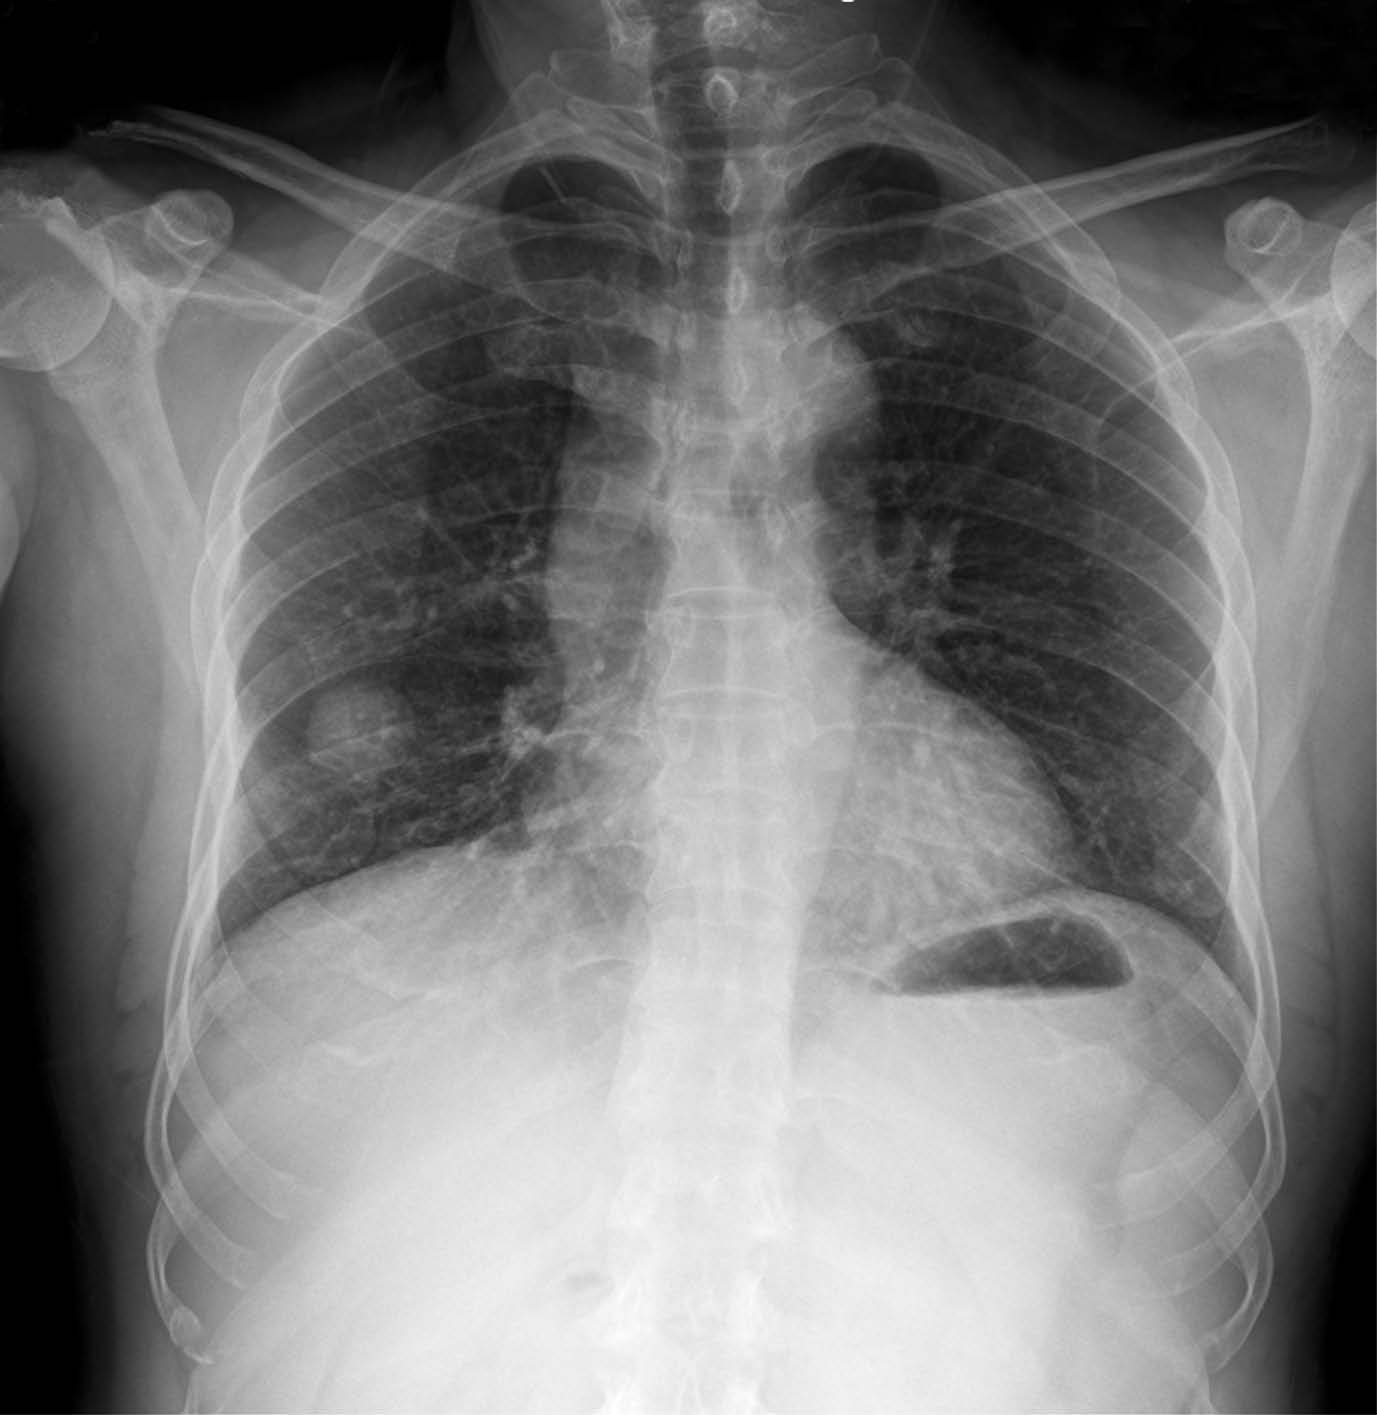
\includegraphics{./images/Image00173.jpg}
 \captionsetup{justification=centering}
 \caption{肺错构瘤}
 \label{fig3-8-11}
  \end{figure} 

\textbf{【病史摘要】}
 男性,54岁。体检时发现右肺下野中带结节影,无任何临床症状。体格检查及实验室检查:无特殊。

\textbf{【X线表现】}
 右肺下野中带见一直径约3cm大小的类圆形结节影,边缘光滑,锐利,无明显分叶及毛刺,病灶内隐约可见散在钙化影。心影大小、形态属正常,主动脉迂曲。双膈光整,肋膈角锐利。

\textbf{【X线诊断】}  右肺下野错构瘤可能性大。

\textbf{【评  述】}
 本病是最常见的肺良性肿瘤,居孤立性肺结节的第三位(5%~8%),仅次于肺癌和肉芽肿性病变。多见于40岁以后,以40~60岁年龄组发病率最高,男性多于女性(2~3∶1)。虽然错构瘤是一种良性肿瘤,但也可缓慢生长。错构瘤起源于小支气管粘膜或粘膜下层的纤维结缔组织内的未分化多项潜能细胞,常位于肺的周边部近胸膜或肺叶间隙处(90%),位于肺门部极少见。肿瘤成分以软骨、粘液瘤样的结缔组织、上皮线样裂为主,还可见脂肪、平滑肌、骨髓、骨或淋巴血管组织。纤维结缔组织可能是错构瘤的原始成分,软骨样组织系由纤维结缔组织转化而来。根据其成分分为软骨型及纤维型,前者较常见,且因含有软骨成分,瘤内可发生钙化,典型钙化方式为爆米花样。脂肪是诊断错构瘤的重要依据,大约有54%的病变内见或多或少的脂肪成分。钙化与错构瘤的大小相关,<2cm的结节检出率约10%,3~4cm大小的肿块检出率约33.3%,大于5cm的病变检出率约75%。错构瘤的X线表现为孤立性圆形或类圆形致密阴影,密度较高,边缘光滑锐利,大小以2.4cm左右占多数。大的错构瘤边缘可见浅分叶状改变。错构瘤可发生于肺任何部位,但绝大多数位于胸膜下区,无卫星灶,也无与肺门相连的条索。

X线诊断错构瘤主要是根据瘤内有钙化。钙化往往不规则地分布于整个球形阴影内,典型者呈特征性爆米花样。除钙化外,错构瘤没有什么其他特点,生长缓慢,长期随访,大小形态变化不大,或略为增大,但不会缩小。

\subsection{肺硬化型血管瘤}

\begin{figure}[!htbp]
 \centering
 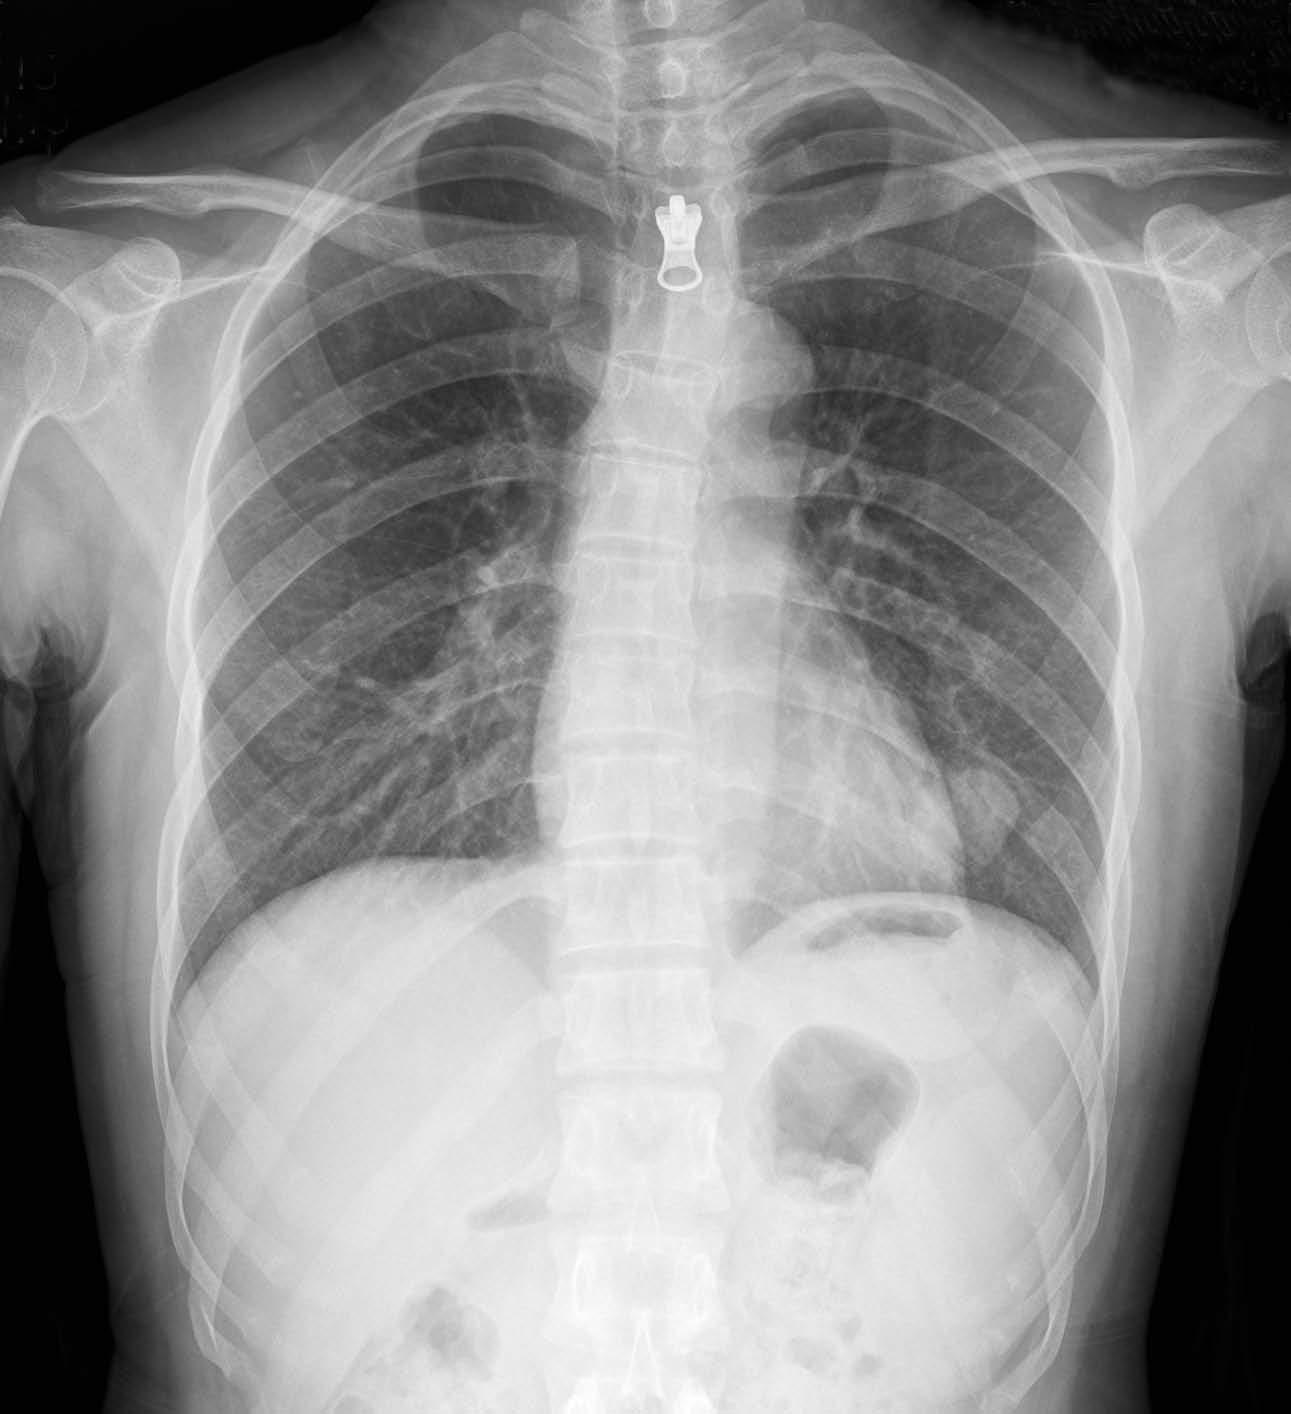
\includegraphics{./images/Image00174.jpg}
 \captionsetup{justification=centering}
 \caption{肺硬化性血管瘤}
 \label{fig3-8-12}
  \end{figure} 

\textbf{【病史摘要】}
 女性,39岁。体检时发现左肺下野占位,无任何症状和体征。

\textbf{【X线表现】}
 左肺下野中带见一类圆形肿块影,直径约4.5cm,边界清晰,轮廓光滑整齐,可见浅分叶,未见明显毛刺,瘤体内部密度均匀,周围未见卫星灶及纤维条索影。心脏大小、形态正常。双侧肋膈角锐利。

\textbf{【X线诊断】}
 左肺下野占位,良性肿瘤可能性大,建议胸部CT(平扫+增强)检查。

\textbf{【评  述】}
 本病例手术切除术后确诊为肺硬化型血管瘤。肺硬化型血管瘤(pulmonary
sclerosing
hemangioma,PSH)是一种少见的肺部良性肿瘤,其来源可能是肺泡Ⅱ型上皮细胞,曾有黄色瘤、纤维黄色瘤、浆细胞肉芽肿、炎性假瘤、肺组织细胞瘤等名称。在WHO(1999)肺肿瘤的新分类中将其正式命名为PSH。PSH的主要病理学特点是纤维组织进行性增生硬化,代替了肺泡结构,毛细血管嵌入,致肺泡内出血,含铁血黄素沉着和泡沫样巨噬细胞反应,最后肺泡壁硬化完全闭塞,形成瘤样结构。肉眼观察肿瘤与周围肺组织界限清楚,多无包膜,质地中等,切面呈灰黄色。PSH主要由2种细胞构成:表面立方细胞和圆形-多角形细胞。光学显微镜下PSH大多数为血管瘤、乳头、实体、硬化4种成分,其中至少3种成分移行混合存在,几乎没有一种成分单独构成的报道,其间可有不同程度的出血及含铁血黄素沉着。因此,也有学者将PSH分为4种组织学亚型:实体型、乳头型、硬化型和血管瘤型。本病好发于中青年女性,以30~50岁多见,瘤体直径多为1~5cm,直径<3cm者占70%,绝大多数表现为肺孤立性结节,4%的患者可多发。患者多无临床症状,几乎均为体检或偶然通过X线胸片或CT发现,有症状者多表现为咳嗽、痰中带血和胸闷。

影像学上,PSH具有常见的肺部良性肿瘤特征,表现为边缘光整、边界清晰的圆形、类圆形肺内结节或肿块,多数位于肺野近肺门的内侧1/2区域内,少数可有轻度分叶,但无毛刺征象。肿瘤内各种组织成分的比例不同决定了CT平扫时的密度差异。将CT平扫病灶内高密度、等密度、低密度区与术后病理对照研究发现,高密度区为瘤体内血凝块充填的海绵状血管瘤区,等密度区为瘤体内的实体部分,低密度区为瘤体内充满黄色液体的囊性区。Sugio等发现PSH囊变的发生率≥20%,与出血有关。PSH出现钙化者占30%~41%,多表现为粗大点片状钙化。相比X线胸片,CT更易检出病灶内的细小钙化灶。

\subsection{肺转移性肿瘤(一)}

\begin{figure}[!htbp]
 \centering
 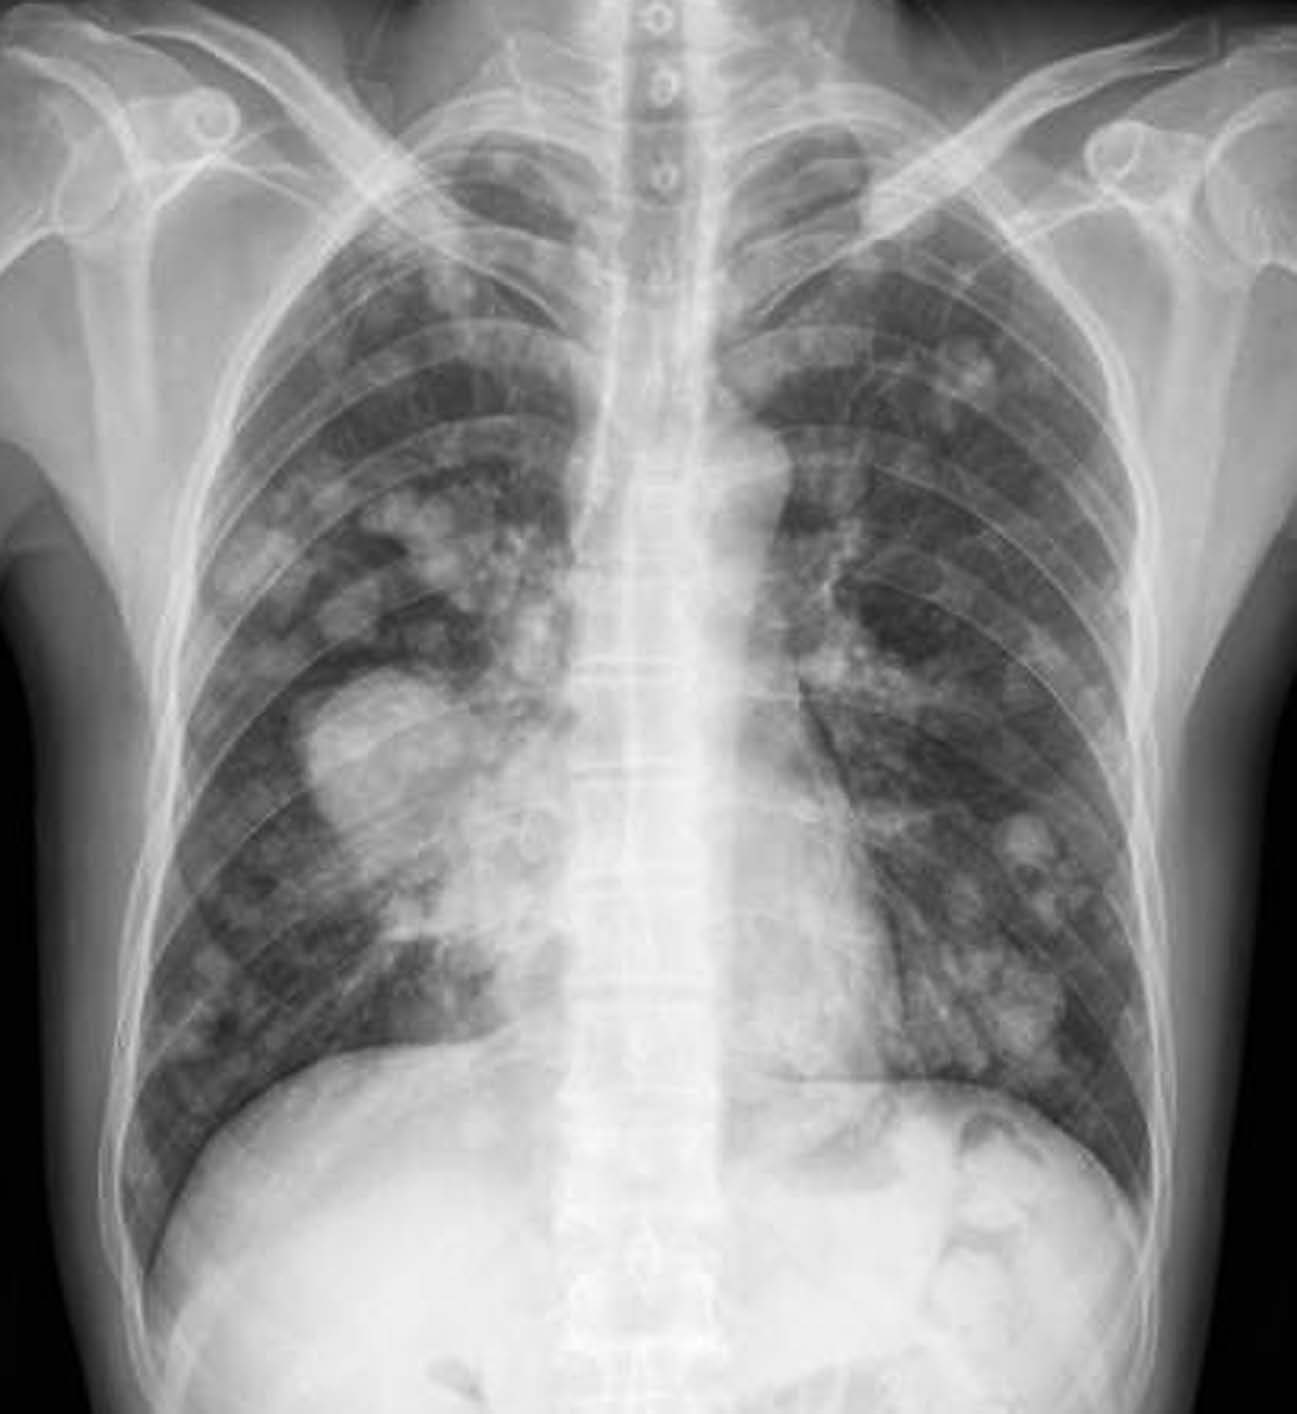
\includegraphics{./images/Image00175.jpg}
 \captionsetup{justification=centering}
 \caption{肺转移瘤(一)}
 \label{fig3-8-13}
  \end{figure} 

\textbf{【病史摘要】}
 男性,56岁。右肺下叶腺癌病史,自觉胸闷、咯血2周入院复查。

\textbf{【X线表现】}
 气管居中。右肺下叶见类圆形肿块影,直径约5cm,边界清晰,无分叶,双肺内见多发大小不等的结节影,似棉花团状,以中下肺野分布为主。双侧肺门见多个钙化淋巴结高密度影。心脏形态大小属正常。双侧肋膈角锐利。

\textbf{【X线诊断】}  右肺下叶周围型肺癌伴双肺多发转移。

\textbf{【评  述】}
 肺部是转移性肿瘤第二发生的部位。其他脏器的恶性肿瘤可以通过血液或淋巴系统转移到肺部。临床症状可分别为原发肿瘤和(或)肺转移所引起。大多数病例有原发肿瘤引起的症状,且原发恶性肿瘤的部位和性质已经证实。本病例曾有肺癌病史。但少数病例可首先发现肺内病变,而原发肿瘤尚不明确。

\subsection{肺转移性肿瘤(二)}

\begin{figure}[!htbp]
 \centering
 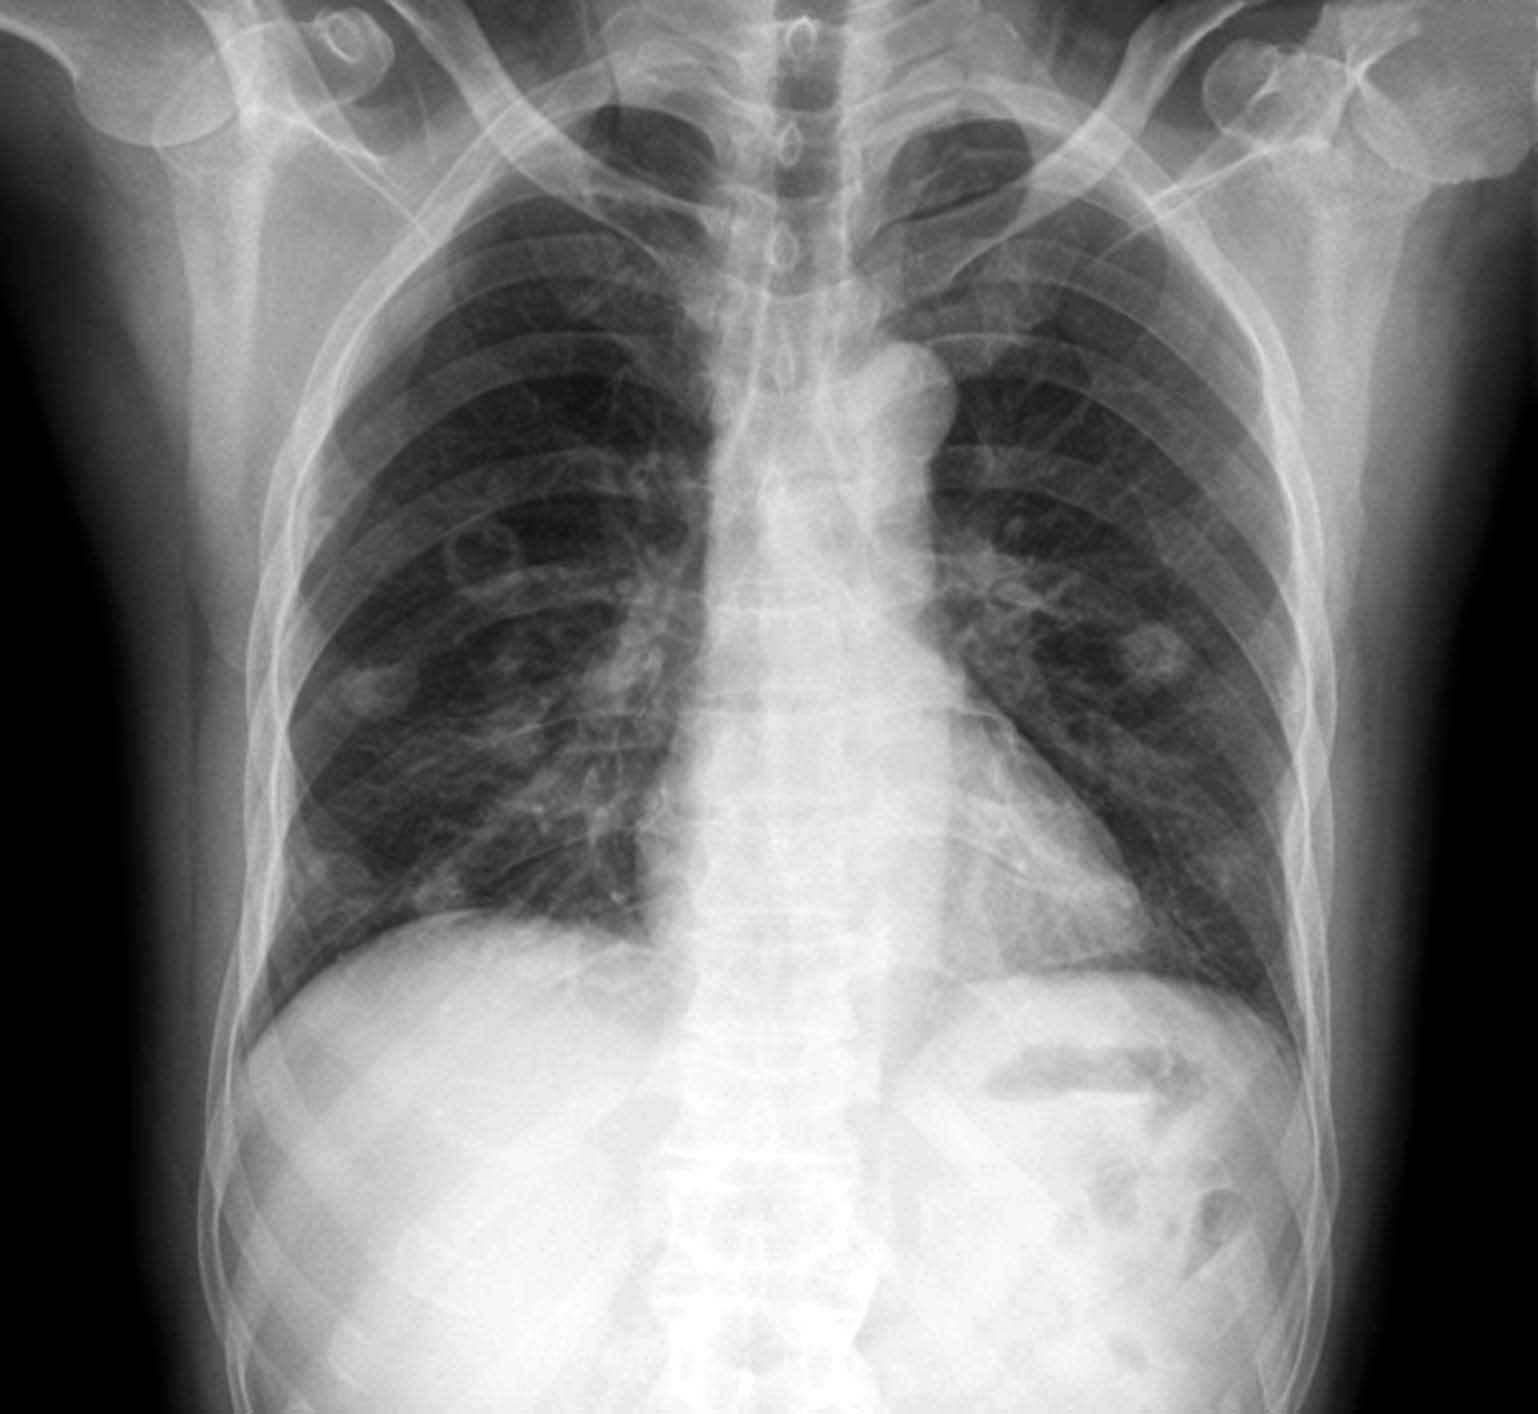
\includegraphics{./images/Image00176.jpg}
 \captionsetup{justification=centering}
 \caption{肺转移瘤(二)}
 \label{fig3-8-14}
  \end{figure} 

\textbf{【病史摘要】}  男性,50岁。直肠癌术后1年,常规复查。

\textbf{【X线表现】}
 气管居中。双肺中下肺野见多个类圆形结节影,边界欠清晰,部分中央见大小不等的圆形透亮影形成。心脏大小形态属正常。双侧肋膈角锐利。

\textbf{【X线诊断】}  直肠癌术后双肺转移伴空洞形成。

\textbf{【评  述】}
 典型肺转移多能明确诊断,但临床常能遇到不典型肺转移,其影像学表现包括:空洞、钙化、单发转移、气胸、气腔模式、支气管内膜转移、肿瘤栓塞、囊性转移等。空洞型肺转移瘤的发生率为4%。X线胸片检查时,以鳞癌发生最多,占空洞型肺转移的69%。但CT检查中,腺癌也常见空洞转移约占9.5%,鳞癌占10%。腺癌和鳞癌发生空洞性转移的概率无显著性差异。淋巴瘤肺转移也可见空洞。空洞形成的原因可能是肿瘤坏死或小支气管的空气活瓣作用。化学治疗可以诱导转移性肺癌形成空洞。

影像学表现为:两肺多发的大小不等、不规则厚壁空洞影,边界清楚,亦可表现多发薄壁空洞;直径1~5cm,常伴有壁结节,越靠近胸膜,空洞越小;大的空洞有多分布于肺中带的倾向,合并气胸并不少见。大多数空洞型肺转移瘤与肺内血行转移结节并存。

\subsection{白血病肺部浸润}

\begin{figure}[!htbp]
 \centering
 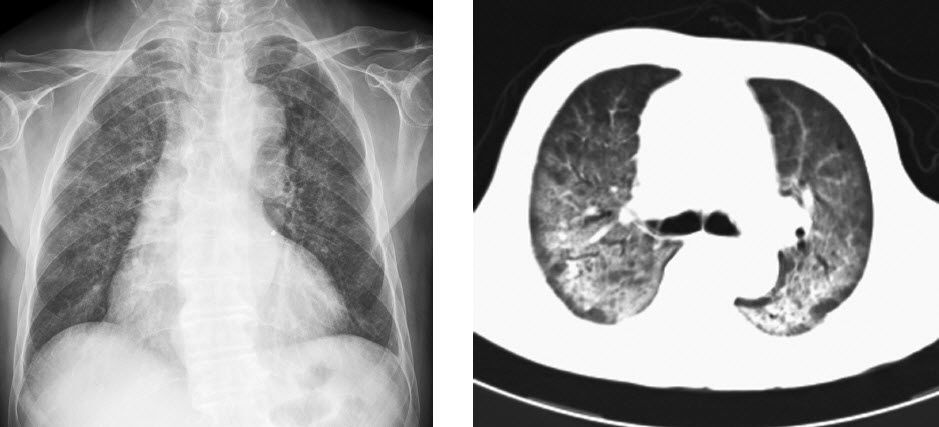
\includegraphics{./images/Image00177.jpg}
 \captionsetup{justification=centering}
 \caption{白血病肺部浸润X线正位和CT肺窗}
 \label{fig3-8-15}
  \end{figure} 

\textbf{【病史摘要】}
 男性,74岁。慢性淋巴细胞性白血病2年余,入院巩固化疗。

\textbf{【X线表现】}
 气管居中。双肺纹理稍增多、增粗,双肺广泛的、沿肺纹理分布的网织阴影,肺野呈磨砂玻璃状;心影呈主动脉型。同一患者CT肺窗示两肺小叶间隔不均匀增厚,呈细网格状,并见大片磨砂玻璃密度影。

\textbf{【X线诊断】}  X线所见,并结合临床,符合白血病肺部浸润。

\textbf{【评  述】}
 尸检发现白血病侵犯肺部者并不少见,但在生前的X线检查,多数的肺部改变是并发感染和心力衰竭所引起的,真正由白血病细胞所引起的浸润甚为少见。白血病直接引起的肺部X线表现最多见的是双侧纵隔肺门淋巴结肿大,约占25%,并较多见于淋巴细胞白血病。白血病肺内侵犯表现为双肺广泛的、沿肺纹理分布和肺野内网织阴影,有时可伴有粟粒状结节影,类似淋巴性转移。本例胸片上仅表现为肺纹理增多及双肺广泛的网织阴影和磨砂玻璃密度影。有时双肺出现多发的圆形结节病变,通常为白血病栓塞所引起,部分病灶融合成团块。25%病例有胸腔积液,可为单侧或双侧,胸腔积液于慢性白血病较多见。

\section{肺尘埃沉着病}

\subsection{硅沉着病(一)}

\begin{figure}[!htbp]
 \centering
 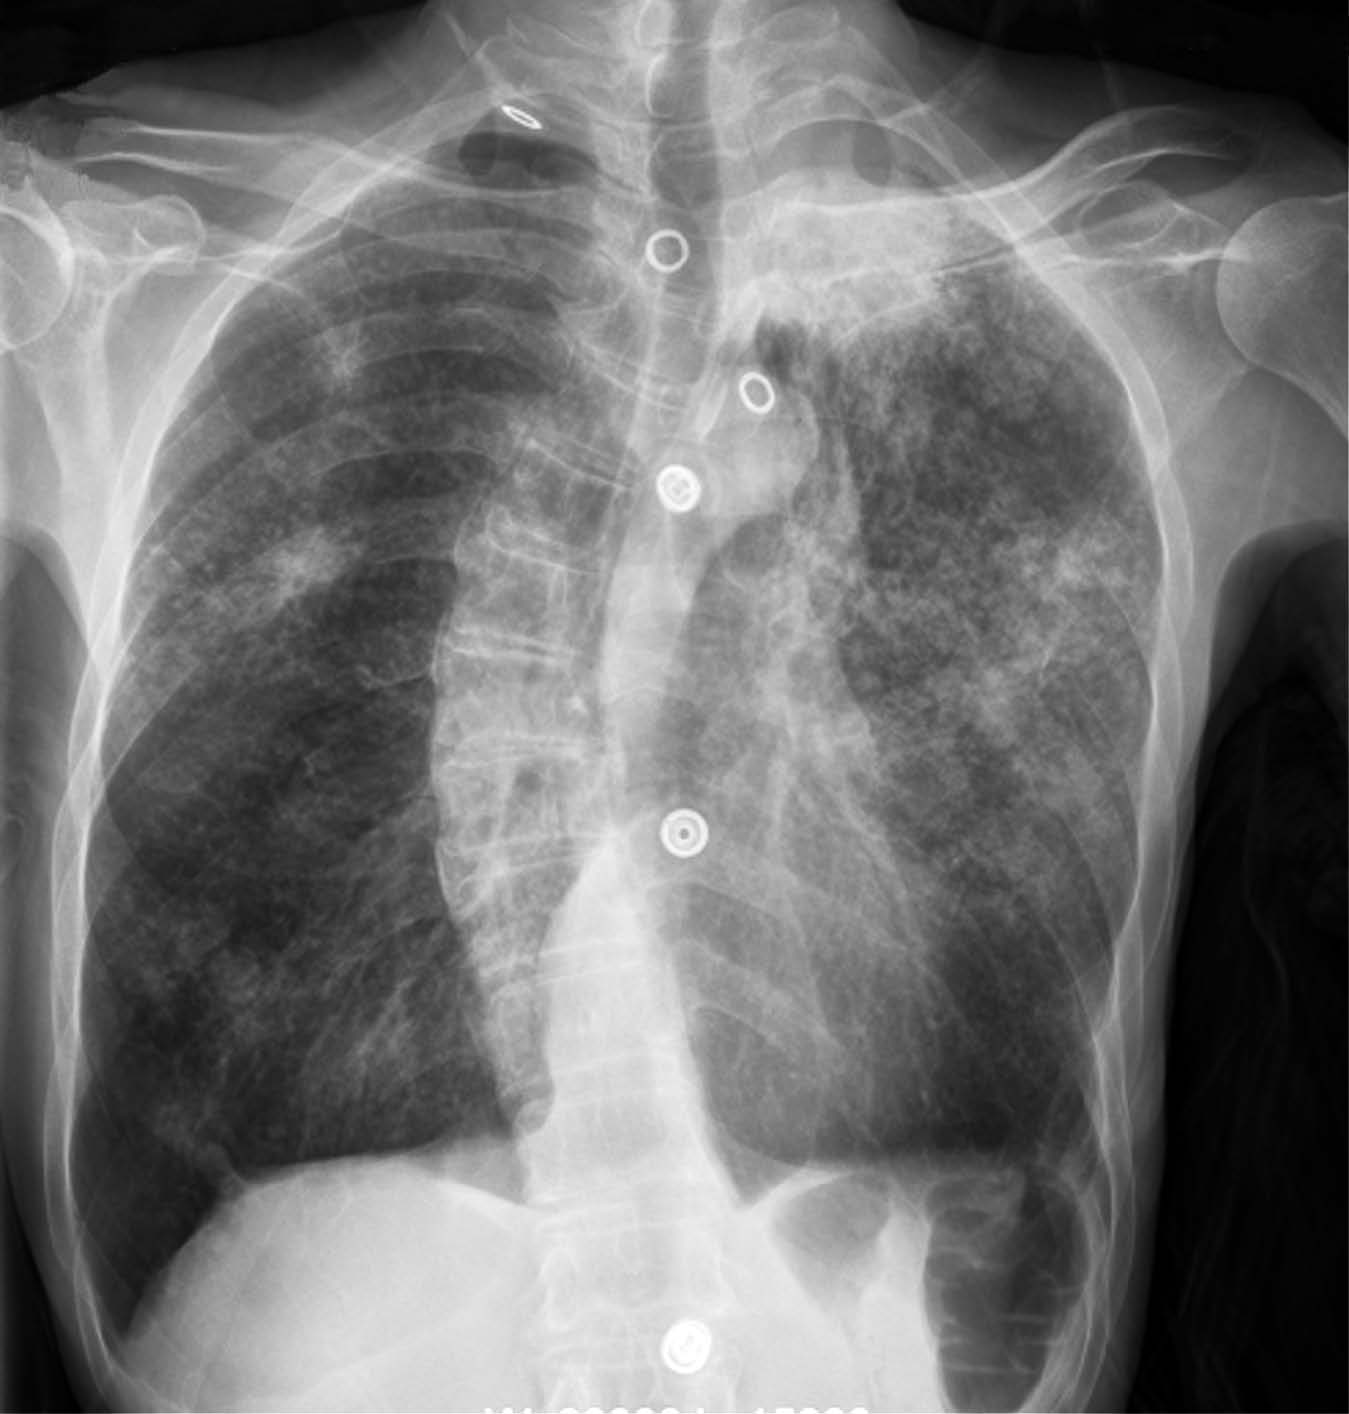
\includegraphics{./images/Image00178.jpg}
 \captionsetup{justification=centering}
 \caption{矽肺Ⅲ期伴肺气肿及双侧胸膜增厚}
 \label{fig3-9-1}
  \end{figure} 

\textbf{【病史摘要】}
 男性,58岁。接触石英粉尘史20年,近10年来感觉呼吸困难。

\textbf{【X线表现】}
 气管向左侧扭曲。脊柱侧弯畸形。两肺透亮度减低,肺纹理增多、增粗,紊乱。双肺内见弥漫性高密度小结节影,以双上中肺为主,部分融合成较大的结节及团块状。左肺尖见较大致密肿块影,边界不清,见伪足征。左侧肺门向上移位,左下肺纹理呈垂柳状。心脏向左侧移位。双侧膈面低平。双侧胸膜增厚粘连,双侧肋膈角锐利。

\textbf{【X线诊断】}
 结合病史,符合硅沉着病(矽肺Ⅲ期)伴肺气肿及双侧胸膜增厚。

\textbf{【评  述】}
 矽肺的矽结节晚期可发生融合,一般常在双侧锁骨下近外周开始,出现一个或几个直径近1cm、边缘往往不甚清楚的增密阴影。其后继续不断地增大、增密,形成宽条、圆形的大块阴影,往往呈纵行排列,其长轴与前肋垂直,范围可超过肺段以至肺叶。此为矽肺大块纤维形成的较为特殊的X线表现,且有一定的诊断价值。通常对称地见于两侧,亦可一侧比较明显,长期局限于一侧者很少见。本例除双肺弥漫性粟粒状高密度矽结节外,双肺中上肺野见多发直径1cm以上的融合性矽结节,甚至于左肺尖可见呈肿块状巨大阴影。

本病例结合患者长期粉尘接触史,肺内弥漫性高密度小结节、肿块、纤维化、肺气肿及胸膜增厚表现,故诊断为矽肺Ⅲ期。

附中华人民共和国卫生部2009年最新发布的《肺尘埃沉着病》诊断标准:

1.肺尘埃沉着病的分类:根据引起肺尘埃沉着病的矿物粉尘的性质,肺尘埃沉着病分为矽肺和尘肺二类。

矽肺------由含游离二氧化硅为主的粉尘引起的矽肺。

尘肺------由含硅酸盐为主的粉尘引起的硅酸盐尘肺,包括石棉肺、水泥尘肺、滑石尘肺、云母尘肺和陶工尘肺等;由煤尘及含碳为主的粉尘引起的尘肺,如煤工尘肺、石墨尘肺和炭黑尘肺;由金属粉尘引起的金属尘肺,如铝尘肺。

有些有机粉尘例如棉尘,虽然也能引起肺部及呼吸道的改变(棉尘肺),且属于职业病的范围,但其病变性质与一般尘肺不同,故不属于尘肺病。

2.最新肺尘埃沉着病的诊断标准:卫生部发布的最新《中华人民共和国肺尘埃沉着病诊断标准》规定,肺尘埃沉着病分为三期。

(1)一期肺尘埃沉着病:是指有总体密集度1级的小阴影,分布范围至少达到2个肺区。

(2)二期肺尘埃沉着病:是指有总体密集度2级的小阴影,分布范围超过4个肺区,或有总体密集度3级的小阴影,分布范围达到4个肺区。

(3)三期肺尘埃沉着病:是指有下列情形之一者:有大阴影出现,其长径不小于20mm,短径不小于10mm;有总体密集度3级的小阴影,分布范围超过4个肺区并有小阴影聚集;有总体密集度3级的小阴影,分布范围超过4个肺区并有大阴影。

所谓肺区是指将肺尖至膈顶的垂直距离等分为三,用等分点的水平线把每侧肺野各分为上、中、下三个肺区。

1、2、3级小阴影是指直径或宽径不超过10mm的阴影;大阴影是指肺野内直径或宽径大于10mm以上的阴影。

所谓密集度是指一定范围内小阴影的数量(应结合肺尘埃沉着病诊断标准片判断)。

\subsection{硅沉着病(二)}

\begin{figure}[!htbp]
 \centering
 \includegraphics{./images/Image00179.jpg}
 \captionsetup{justification=centering}
 \caption{矽肺Ⅲ期伴肺动脉高压}
 \label{fig3-9-2}
  \end{figure} 

\textbf{【病史摘要】}
 男性,58岁。粉尘接触史20余年,呼吸困难伴咯血半年来医院检查。

\textbf{【X线表现】}
 气管居中。双侧肺门影明显增大、增浓,伴钙化点。双肺纹理增多、增粗,紊乱。双侧中下肺野见数枚高密度小结节状致密影。右肺下叶动脉干增粗,右肺下叶远端纹理呈残根状,左肺下叶纹理呈垂柳状。双侧叶间裂明显增厚。心脏形态大小属正常。双侧肋膈角稍钝。

\textbf{【X线诊断】}
 结合病史,符合双侧硅沉着病(矽肺Ⅲ期)伴肺动脉高压表现。

\textbf{【评  述】}
 本病例后行肺动脉CT血管造影,发现肺门肿块非单纯肿大淋巴结,而是双侧肺门部矽结节合并肿大淋巴结、纤维化后形成肿块,包裹了双侧肺门大血管,形成肺动脉高压,虽然周围肺野内矽结节较少,故诊断硅沉着病(矽肺Ⅲ期)伴肺动脉高压。

\section{其他原因肺疾病}

\subsection{肺结节病}

\begin{figure}[!htbp]
 \centering
 \includegraphics{./images/Image00180.jpg}
 \captionsetup{justification=centering}
 \caption{肺结节病}
 \label{fig3-10-1}
  \end{figure} 

\textbf{【病史摘要】}
 女性,56岁。体检时发现双侧肺门增大,追问病史,偶有胸闷不适。

\textbf{【X线表现】}
 气管居中。双侧肺门增大、增浓。增大的肺门周围可见斑片条索影。心脏形态大小属正常。右侧中纵隔增宽。双侧肋膈角锐利。

\textbf{【X线诊断】}  双侧肺门及右侧气管旁淋巴结肿大-结节病可能性大。

\textbf{【评  述】}
 结节病属多器官受累的肉芽肿性疾病。发病年龄分布呈双高峰:第一高峰为青年期,第二高峰为50岁以上的中年期。女性发病略高于男性。该病病因目前尚不明确。全身以胸内浸润为主,86%~97%存在肺门淋巴结肿大,31%~48%有肺内浸润。结节病的病理学特征性表现是在淋巴管管内或淋巴管周围分布的非干酪样坏死肉芽肿。临床表现缺乏特异性,且部分患者无症状而为偶然体检发现。

目前临床诊断要点:①多系统临床表现。②非干酪样坏死肉芽肿病理改变。③除外其他肉芽肿性疾病。结节病的典型X线胸片表现为右侧气管旁、右肺门及左肺门淋巴结肿大,即1-2-3征;但仅有双侧肺门淋巴结肿大时,呈土豆征。结节病二期肺内弥漫性小结节呈网格影改变亦常见。针对缺乏临床表现的病例,胸片也起到提示作用。此外,胸片分期对了解疾病的严重程度、发展阶段和提示预后方面也都有重要意义。5%~15%X线胸片表现正常但在组织学上都发现肉芽肿。而CT的诊断信息高于胸片2倍,更重要的是在有把握的CT诊断中,93%和最后结果一致,而胸片中23%最终证明不准确。因此,相对而言,CT检查的意义高于X线胸片。

结节病需鉴别的疾病有多种,以淋巴结肿大为主的需与淋巴瘤、结核和转移鉴别。而肺内弥漫性小结节表现时需与癌性淋巴管炎、粟粒性结核、过敏性肺泡炎等相鉴别。如前所述,根据淋巴结、肺内小结节的分布、形态等可进行区分。

\subsection{特发性肺间质纤维化}

\begin{figure}[!htbp]
 \centering
 \includegraphics{./images/Image00181.jpg}
 \captionsetup{justification=centering}
 \caption{特发性肺间质纤维化}
 \label{fig3-10-2}
  \end{figure} 

\textbf{【病史摘要】}
 女性,53岁。自觉胸闷4个月,咳嗽、胸痛3天,活动后胸闷加重,咳少量白痰,无明确发热。体格检查:一般情况可,两肺听诊呼吸音急促粗糙,两侧下肺部闻及湿啰音,心音正常。

\textbf{【X线表现】}
 两侧中下肺野见弥漫性纤维条索状影,以下肺为著,两侧肋膈角处病变有融合趋势,两侧心缘及纵隔面毛糙。心影形态大小尚属正常范围。

\textbf{【X线诊断】}  两肺特发性肺间质纤维化。

\textbf{【评  述】}
 本病又称寻常型间质性肺炎(UIP),是特发性间质肺炎中最常见的类型。组织学上,特发性肺间质纤维化的特点是肺实质、间质性炎症,成纤维细胞增生,间质性纤维化和蜂窝状的斑片状不均匀分布,以沿胸膜下为主,且各时相不一。好发年龄为50~70岁,男性多见。临床表现为进行性呼吸困难、干咳和乏力。肺功能检查呈中重度限制性通气障碍,肺弥散功能下降。胸片表现与临床表现常不一致。20%~30%的患者伴有胶原血管性疾病,硬皮病和类风湿性关节炎也较为常见。激素治疗效果差,预后差,病死率高,中位生存期为3~6年。X线胸片最常见表现为肺容积下降,80%出现肺外周网格影,以背侧和肺基底部最显著。早期两下肺外周见不规则线样或网格状影;晚期两下肺外周见粗网格状密度影或网格结节混杂密度灶;终末期见蜂窝样改变和小囊样透亮影。HRCT的典型表现是由肺尖向肺基底逐渐加重和胸膜下区的间质纤维化,包括不规则线样影、网格状改变、牵拉性支气管扩张及大囊性蜂窝等;其他包括代表活动性肺泡炎症的磨砂玻璃密度影,但范围和程度有限。寻常型间质性肺炎/特发性肺间质纤维化最主要的HRCT特征是“肺尖-底分布呈梯度分布”的较严重肺间质纤维化表现。

美国胸部学会(ATS)和欧洲呼吸学会(ERS)提出,在无开胸活检证实时,诊断特发性肺间质纤维化需要符合4项主要标准和4项次要标准中的3项。4项主要标准包括:①排除诸如接触有害物质、药物和结缔组织等已知原因的浸润性肺部。②肺功能检查有限制性通气异常和气体交换障碍。③HRCT见两肺基底部有网状影及少量磨砂玻璃密度影。④经支气管活检或支气管灌洗未发现其他疾病证据。4项次要标准包括:①年龄>50岁。②起病隐匿的用力性呼吸困难。③病程3个月或更长。④两肺基底部有吸气时的爆裂音。

\subsection{肺泡微石症}

\begin{figure}[!htbp]
 \centering
 \includegraphics{./images/Image00182.jpg}
 \captionsetup{justification=centering}
 \caption{肺泡微石症}
 \label{fig3-10-3}
  \end{figure} 

\textbf{【病史摘要】}
 男性,30岁。呼吸困难10余年,进行性加重约5年,伴干咳。

\textbf{【X线表现】}
 气管居中。双肺野内见弥漫性分布的高密度粟粒状小结节影呈暴风沙样,伴肺纹理增多、增粗,紊乱,呈面纱征。右侧叶间裂,左侧心缘、双侧膈面呈致密高密度线状影。心脏形态、大小属正常。双侧肋膈角显示不清。

\textbf{【X线诊断】}
 结合临床,肺泡微石症可能,建议HRCT检查及肺穿刺活检。

\textbf{【评  述】}
 本病是一种罕见的、以肺泡内多发微小结石沉积及继发间质纤维化为特征的肺部慢性疾病。病因至今不明,50%~77%有家族发病倾向,均限于同胞之间,考虑为一种常染色体隐性遗传性疾病。另认为与先天性的代谢紊乱及异常刺激或感染导致渗出后钙盐钙化有关。可累及各年龄段,以30~50岁居多,性别分布无差异。病理改变主要为无数直径0.01~3mm、多为1mm左右的同心圆状钙化小体沉积于肺内,绝大多数存在于肺泡腔内,也可在肺泡壁、细支气管与肺间质内。大体标本切面呈细砂纸状纹理。主要侵犯两中下肺,使病肺变硬,重量明显增加,触之沙砾感。初期肺泡壁正常,进展期间质纤维化和巨细胞形成使肺泡壁增厚,出现肺气肿和肺大泡,最终导致肺动脉高压和肺源性心脏病,多死于呼吸衰竭。影像学改变明显而临床症状轻微是肺泡微石症的一大特点。疾病呈缓慢进行性发展,病程可达10~20年。早期可出现轻度干咳、胸闷,随疾病进展,部分病例可出现气促、咯血、杵状指甚至发绀。肺功能检查结果取决于微结石占据肺泡的多少而定,一般肺活量与弥散能力可以降低。血生化分析钙、磷均可在正常范围内,偶尔痰内可检出微结石。

X线胸片表现为:①病变较轻者,可仅表现两肺散在分布的微小结节,其表现类似含铁血黄素沉着症或尘肺等,易误诊。②鱼子样或暴风沙样改变,病变从上至下逐渐密集,尤以两肺底部呈一片致密,心缘及膈面被掩盖(即出现心缘消失征)。③白肺样表现,两肺中、下肺野甚至全肺呈一片白实,肺结构及纵隔缘甚至肋骨均被完全掩盖,见于病情较重者。④两肺(尤以中、下肺野为著)呈高密度网状影伴散在高密度点状阴影,使整个肺野呈“面纱样”改变,此型系微结石沉积于小叶间隔等肺间质内较多所致。需鉴别的疾病包括:尘肺、含铁血黄素沉着、粟粒性肺结核及热带嗜酸粒细胞增多症等弥漫分布间质结节病变。依据分布特点,结节密度较高、肺内影像学改变与临床症状不符,且病变进展缓慢,随访变化不大,以及缺乏粉尘接触史,血液钙、磷代谢无异常等方面有助于诊断。

\subsection{肺泡蛋白沉积症}

\begin{figure}[!htbp]
 \centering
 \includegraphics{./images/Image00183.jpg}
 \captionsetup{justification=centering}
 \caption{肺泡蛋白沉积症}
 \label{fig3-10-4}
  \end{figure} 

\textbf{【病史摘要】}
 男性,36岁。干咳,偶尔咯出胶状物约数月余,近感气急、乏力。经肺泡灌洗,灌洗液呈乳白色牛奶样,并有沉积物。过碘酸希夫反应(PAS反应)呈阳性。

\textbf{【X线表现】}
 气管居中。双肺野中下肺野见大片状边界尚清的致密影,密度不均,以肺野中内带分布为主。心脏形态大小属正常。双侧肋膈角锐利。

\textbf{【X线诊断】}
 双肺中下肺野大片实变,结合临床-肺泡蛋白沉积症,建议HRCT检查。

\textbf{【评  述】}
 肺泡蛋白沉积症是一种以肺泡腔内被过碘酸希夫(periodic acid
Schiff,PAS)染色阳性的脂蛋白样物质充盈为特征,伴有邻近间质炎性反应的浸润性肺病。发病机制不明,大多为特发性。发病年龄集中在30~50岁(2/3),男性多于女性(4∶1)。肺泡蛋白沉积症是一个肺表面活性物质稳态破坏和肺免疫功能损伤的病理生理过程,并与吸烟强烈相关。肺泡腔被过PAS染色阳性的脂蛋白样物质充盈取代,伴有邻近小叶内及小叶间间隔水肿、炎性反应或纤维化。临床症状常较轻或为隐袭性,包括干咳、活动时呼吸困难相对多见,胸痛、低热、不适感少见。当肺部出现弥漫性结节状病变或类似炎症或肺水肿时,应想到肺泡蛋白沉积症可能,特别是病变发展缓慢,抗生素、糖皮质激素治疗无效时将提示本病。HRCT对诊断有较大帮助。最特征性的HRCT表现是双侧肺内磨砂玻璃样密度影伴有光滑的小叶间隔增厚;磨砂玻璃样密度区域常与正常肺实质区域界线清晰,呈地图状分布。确诊主要通过纤维支气管镜肺活检或肺泡灌洗液PAS染色。

肺泡蛋白沉积症以结节样病变为主时,应与弥漫型肺泡细胞癌、肺结节病、肺特发性含铁血黄素沉着症及转移癌相鉴别,但鉴别较困难。然而,结节病常伴有肺门和周围淋巴结肿大,肺特发性含铁血黄素沉着症患者发病年龄较小,一般在15岁以下,有反复咯血史,肺部阴影变化较快,在2~3日内可明显吸收;肺泡细胞癌和转移癌的发病年龄偏大,经1~2个月病灶数量增多,病灶增大。这些有助于与肺泡蛋白沉积症相鉴别。当病灶类似于肺水肿,但无心脏增大及肺瘀血改变,均不易混淆。病灶类似于大叶型肺炎,但无发热,且变化缓慢,应想到该病。

\subsection{肺组织细胞增生症X}

\begin{figure}[!htbp]
 \centering
 \includegraphics{./images/Image00184.jpg}
 \captionsetup{justification=centering}
 \caption{肺组织细胞增生症X}
 \label{fig3-10-5}
  \end{figure} 

\textbf{【病史摘要】}  女性,2岁。间隙性发热8天,有咳嗽、流涕。

\textbf{【X线表现】}
 气管居中。双肺中下野纹理增多、增粗,两肺散在斑片状致密影。心影形态大小属正常。右侧第6后肋增粗,局部骨质破坏(同一患者头颅CT显示右侧颞骨局部骨质破坏)。

\textbf{【X线诊断】}  肺组织细胞增生症X可能性大。

\textbf{【评  述】}
 本病为组织细胞浸润网状内皮系统所致,包括勒雪病、韩-雪-柯病及嗜酸性肉芽肿三种病。可浸润骨、肝、脾、淋巴结及肺。勒雪病多累及肝、脾,其次为肺,骨受累较少见。韩-雪-柯病、嗜酸性肉芽肿主要累及骨骼。勒雪病发病急、病程短,多见于婴儿,以发热和肝脾肿大及皮疹为特征。韩-雪-柯病可发生于儿童及青年,呈慢性过程。临床三大症状是突眼、多饮多尿及膜样化骨破坏。嗜酸性肉芽肿多见于成人,骨质破坏可发生在骨骼的任何部位。常见症状为慢性咳嗽和轻度呼吸困难,如未并发感染,一般情况下无痰,可有胸痛,当肺囊泡破裂时发生自发性气胸,部分患者可有轻中度发热、咯血、夜汗、食欲减退、体重减轻,也有少数发生骨损害及尿崩症等。

肺部X线表现的病理基础是组织细胞浸润肺间质。X线胸片可表现为双肺下野或中下野肺纹理增粗,网状及粟粒状或小结节阴影多见。早期以细胞浸润为主,晚期可发展为肺间质纤维化,并可出现蜂窝肺。

本病的X线影像缺乏特征性,应与肺淋巴管平滑肌瘤、结节病、特发性肺间质纤维化、肺泡细胞癌等鉴别。肺淋巴管平滑肌瘤病好发于育龄期妇女,影像学上表现为全肺均匀分布大小不等的薄壁囊肿,较有特征性。肺结节病与肺组织细胞增多症的呼吸道症状与全身症状都十分轻微或无症状,两者早期均有自行缓解或痊愈的可能,两者虽为弥漫性阴影,但胸部结节病绝大多数有两侧对称性肺门淋巴结肿大,且其他脏器常同时受累,如有皮肤和浅表淋巴结受累,活检即可诊断。特发性肺间质纤维化(IPF)与肺组织细胞增多症两者都为局限于肺部的疾病,但临床症状和预后迥然不同,两者都有弥漫性阴影,但肺组织细胞增多症早期为小点、片状阴影混杂,分布比较均匀,纤维化程度较轻,肺体积无明显缩小;而IPF阴影首先出现在中下肺野外带,病变集中在中下肺,使下肺缩小,肺门下降并向纵隔靠拢,病变持续加重,晚期形成蜂窝肺,肺体积明显缩小,膈肌上抬。肺泡细胞癌早期临床症状亦很轻微,随病情发展可出现咳嗽、咳大量白色泡沫痰、呼吸困难,阴影早期可发生在一侧肺,然后逐渐向对侧发展,而肺组织细胞增多症开始即为对称性阴影,阴影虽多,但临床症状轻微,肺泡细胞癌痰中可找到癌细胞。

由于本病的肺部病变经过缓慢,可持续数年不见吸收,一般没有纵隔肺门淋巴结肿大征象,故患者也可无呼吸道症状或症状轻微而不能引起重视,肺部无阳性体征,而仅于胸部X线检查时发现,实验室检查无帮助,常为正常值,部分患者白细胞增高,中性粒细胞增多,嗜酸粒细胞很少能在血液中发现,免疫学检查可正常。当患者出现上述病史、实验室检查及胸部X线影像时,应想到本病的可能,及时行肺组织活检。

\subsection{急性呼吸窘迫综合征}

\begin{figure}[!htbp]
 \centering
 \includegraphics{./images/Image00185.jpg}
 \captionsetup{justification=centering}
 \caption{急性呼吸窘迫综合征}
 \label{fig3-10-6}
  \end{figure} 

\textbf{【病史摘要】}
 男性,45岁。发热3天后出现呼吸困难,并伴烦躁不安。体格检查:呼吸急促,35次/分,胸部可闻及满肺湿啰音。动脉血氧分压6.5kPa。

\textbf{【X线表现】}
 气管居中。双肺野内满布小斑片状密度增高影,中下肺野大片状融合。左心缘被遮挡,显示不清。双侧膈面及肋膈角模糊。

\textbf{【X线诊断】}  急性呼吸窘迫综合征。

\textbf{【评  述】}  急性呼吸窘迫综合征(acute respiratory distress
syndrome,ARDS),是指临床各科多种原发疾病在抢救或医治过程中发生的急性、进行性、缺氧性呼气困难。常见原因有:①休克:感染性、出血性和过敏性休克。②严重外伤:多发性骨折、内脏破裂、烧伤等。③严重感染:细菌性、病毒性感染。④其他原因:如脂肪栓塞、胃液吸入、毒气吸入、药物中毒、体外循环术后等。X线表现随发病时间不同而变化,可分为4期:①在发病12~24小时内,双肺纹理增多、增粗、模糊,可伴有小斑片状阴影。②中期:在发病后1~3天,肺内出现斑片状和大片状融合阴影,多数为双肺分布,少数发生在一侧,外带病变常比内带严重。③晚期:在发病3天以后,双肺广泛分布片状阴影,但肺组织晚期实变时,双肺普遍变白,心影轮廓消失,故这种改变称为白肺,是诊断该病的重要征象。④恢复期:在发病7天后,X线阴影逐渐消失,少数患者可出现肺纤维化,诊断本病必须与病史、临床表现及血气分析相结合,并需除外心源性和非心源性肺水肿。

\subsection{肺淋巴管肌瘤病}

\begin{figure}[!htbp]
 \centering
 \includegraphics{./images/Image00186.jpg}
 \captionsetup{justification=centering}
 \caption{肺淋巴管肌瘤病}
 \label{fig3-10-7}
  \end{figure} 

\textbf{【病史摘要】}
 女性,45岁。突发左侧胸痛、胸闷1天,近5年来多次气胸史。

\textbf{【X线表现】}
 气管居中。左上侧胸腔内可见压缩的肺边缘及弧形无肺纹理结构带(箭头1),左肺压缩10%左右;双肺野内纹理清晰,双下肺野内带见类圆形边界不清的透亮影(箭头2、3)。心影形态、大小属正常。左侧肋膈角稍钝,右侧锐利。同一患者胸部CT显示左侧少量气胸,两肺内见多发散在肺气囊影,以左肺明显。

\textbf{【X线诊断】}
 左侧气胸;双肺多发气囊影;结合临床,淋巴管肌瘤病不除外,建议CT检查。

\textbf{【评  述】}
 本病例经胸腔镜活检证实。淋巴管肌瘤病是一种罕见性原因不明的疾病,好发于女性,尤以17~50岁妇女最常见,累及肺内外。有研究认为肾脏的发病早于肺部4~9年,但多数患者以肺内改变为主。具体发病机制尚不明确,推测与性激素有关。另报道结节性硬化(TSC)女性伴发肺淋巴管肌瘤病比例可高达34%,且两者基因变异存在一定联系,故认为淋巴管肌瘤病是TSC的一种顿挫型,究竟两者关系如何仍有待研究。

淋巴管肌瘤病基本病理特征为淋巴管、小血管、小气道及其周围类平滑肌细胞的进行性增生,形成显微镜下结节,引起局部管腔结构的狭窄或阻塞。在肺内小气道因增生结节引起细支气管活瓣性阻塞,空气滞留,远端肺泡扩大融合而成,形成囊腔性病变。肺小静脉阻塞造成肺水肿、肺出血及含铁血黄素沉积。淋巴管或胸导管增厚阻塞引起淋巴回流障碍,淋巴管破裂而致乳糜胸、腹水;同时伴有肺门、纵隔及后腹膜淋巴结肿大,还可出现纵隔、腹腔、后腹膜淋巴管瘤。而腹、盆腔异常表现发生率据统计高达76%,表明该病属多部位受累疾病。大多数病例有呼吸困难、气胸和(或)咳嗽。从出现症状到确诊的间隔时间通常为3~5年。在病程中,80%的病例发生气胸,30%~40%出现血色痰或间歇性咯血。几乎全部病例都有肺功能异常。X线胸片往往难以显示肺的多发小囊状透亮影特征,表现为网状、网状结节状、粟粒和蜂窝等,50%的病例有气胸的X线证据。本病例双侧肺底部可见两个融合性大的类圆形透亮影。胸部HRCT是明确该病的主要方法。HRCT特征性表现为两肺广泛分布的小囊状低密度影。囊壁多<3mm,囊腔间组织相对正常。随病程进展,囊状影有增大、增多趋势,部分融合成类肺大疱状。当胸膜下囊腔破裂时,可导致气胸。当囊腔间肺组织出现磨砂玻璃样密度影时,可能代表出血区。由于腹部改变并非少见,建议对怀疑淋巴管肌瘤病的患者常规行腹部及盆腔增强CT检查。

影像学上需鉴别的疾病包括小叶中央型肺气肿、组织细胞病X、结节硬化症(TSC)等。当年轻、育龄期妇女肺内出现多发囊状空腔性病变时,伴有呼吸困难,应考虑到肺淋巴管肌瘤病可能。而肺气肿多发生于老年患者,且多伴有慢性支气管炎表现及牵引性支气管扩张,可资鉴别。其他需鉴别的两种疾病,较肺淋巴管肌瘤病更罕见,HRCT技术、结合其他系统特征性表现可资诊断。

\section{胸膜病变}

\subsection{胸腔积液(一)}

\begin{figure}[!htbp]
 \centering
 \includegraphics{./images/Image00187.jpg}
 \captionsetup{justification=centering}
 \caption{胸腔积液(一)}
 \label{fig3-11-1}
  \end{figure} 

\textbf{【病史摘要】}
 男性,30岁。持续性胸痛3个月,伴头昏、乏力,并时有盗汗。体格检查:左侧呼吸运动减弱,语颤减低,左下肺叩诊实音,听诊左下肺呼吸音消失,右下肺呼吸音减弱。

\textbf{【X线表现】}
 气管居中。左中下肺野见大片状致密影,上缘外高内低,余肺野清晰。纵隔无明显移位。心影形态、大小属正常。左侧膈面、左侧肋膈角消失;右侧膈面、肋膈角正常。

\textbf{【X线诊断】}  左侧胸腔积液(中等量)。

\textbf{【评  述】}
 胸腔积液是胸腔内液体溢出的积聚。产生的病因各异,可以是结核性、化脓性、肿瘤性、外伤性或心肾疾病所致。液体的性质不一,可以是渗出液、漏出液、脓液、血液、乳糜液或混合性液体。X线诊断只能确定积液的部位和程度,一般不能确定其性质。根据临床病史、超声检查可与肺不张、肺炎及胸腔内巨大肿瘤等鉴别。

\subsection{胸腔积液(二)}

\begin{figure}[!htbp]
 \centering
 \includegraphics{./images/Image00188.jpg}
 \captionsetup{justification=centering}
 \caption{胸腔积液(二)}
 \label{fig3-11-2}
  \end{figure} 

\textbf{【病史摘要】}
 男性,30岁。发热、胸痛1周,胸闷气促1天入院。体格检查:左侧胸廓饱满,呼吸运动减弱,语颤减低,叩诊实音,听诊呼吸音消失。

\textbf{【X线表现】}
 气管向右侧移位。左侧胸腔见大片密度均匀的致密影,充满整个左侧肺野。右侧肺野清晰。纵隔向右侧移位。心影形态、大小因左心缘被遮盖,无法判断。左侧膈面及肋膈角消失,右侧肋膈角变钝。

\textbf{【X线诊断】}  左侧大量胸腔积液。

\textbf{【评  述】}
 胸腔积液包括游离性和包裹性积液。游离性胸腔积液:少量积液(200~300ml)时因重力关系,液体常积于胸膜腔最低处的肋膈角。侧位片后肋膈角变钝,胸片肋膈角变钝,呈一楔状致密影。中等量积液正位胸片可见下半肺野大片密度均匀的致密影,正常膈肌弧线影消失。其上缘呈一抛物线状,其外侧高于内侧,弧线由外上方倾斜向内下方,侧位胸片可见积液致密影上缘呈前后胸壁高而中央凹下的弧线。如胸腔积液同时伴有下叶肺不张或肿瘤,则正位片的上缘弧线成为内高外低的相反形态。大量积液使一侧肺野呈广泛大片状致密影,肋间隙增宽,纵隔推向对侧,气管亦向健侧移位,患侧膈肌下降。如有一侧大量积液而纵隔无移位,需考虑同时有肺不张,或是由于纵隔固定之故。

\subsection{气胸}

\begin{figure}[!htbp]
 \centering
 \includegraphics{./images/Image00189.jpg}
 \captionsetup{justification=centering}
 \caption{气胸}
 \label{fig3-11-3}
  \end{figure} 

\textbf{【病史摘要】}
 男性,17岁。左侧胸痛6小时入院。体格检查:左肺呼吸音减低。

\textbf{【X线表现】}
 气管向右侧移位。左侧肺野可见肺外带胸壁间狭长透亮带及内缘萎陷肺线样致密边缘。余肺野清晰。心影形态、大小正常。左侧膈面下降,双侧肋膈角锐利。

\textbf{【X线诊断】}  左侧气胸,压缩<50%。

\textbf{【评  述】}
 气胸是因为壁层或脏层胸膜破裂后,空气进入胸膜腔而形成。前者常为胸壁创伤或人工穿刺所致;后者则是肺表面的破损,如接近脏层胸膜的肺大疱、肺气肿破裂以及肺结核或其他肺部感染引起肺组织坏死而使脏层胸膜溃破,有些是突然用力、喷嚏或剧烈咳嗽所致。自发性气胸多见于瘦长体形的年轻人。

\subsection{脓气胸}

\begin{figure}[!htbp]
 \centering
 \includegraphics{./images/Image00190.jpg}
 \captionsetup{justification=centering}
 \caption{脓气胸}
 \label{fig3-11-4}
  \end{figure} 

\textbf{【病史摘要】}  男性,63岁。左下肺癌切除术后6天,发热、胸痛3天。

\textbf{【X线表现】}
 左下肺癌切除术后改变。左侧胸廓缩小,左侧肋间隙略变窄,气管居中,左侧下胸腔见密度均匀致密影紧贴左侧膈肌上及左外侧胸壁,其上部见透亮的气液平。右侧肺纹理清晰。心影形态大小正常,主动脉迂曲。左膈肌升高,左侧肋膈角消失,左下胸膜增厚,右侧肋膈角锐利。

\textbf{【X线诊断】}  左下肺癌切除术后改变,左侧包裹性脓气胸。

\textbf{【评  述】}
 脓气胸可为肺部炎症,如肺脓肿、肺结核等并发症或胸壁创伤后感染所致。包裹性脓气胸多在肺野外侧,由于具有空腔及液气平,可类似肺内空洞,但包裹性脓气胸的X线特点是液平面比较长大,空腔壁则较不明显,缺乏一般肺内脓肿的炎性厚壁。且不受肺叶解剖的限制。又由于脓气胸的壁由增厚的胸膜所构成,故在切线位上空腔的壁总是与胸壁成钝角,而贴着胸壁的肺内脓肿则与胸壁成锐角。

\subsection{液气胸}

\begin{figure}[!htbp]
 \centering
 \includegraphics{./images/Image00191.jpg}
 \captionsetup{justification=centering}
 \caption{液气胸}
 \label{fig3-11-5}
  \end{figure} 

\textbf{【病史摘要】}
 男性,22岁。右侧胸痛、呼吸困难2天。体格检查:右侧呼吸音减弱,心率90次/分,律齐。

\textbf{【X线表现】}
 气管居中。右肺受压向肺门部萎陷,右侧胸腔透亮度增高,压缩的肺边缘与胸廓间可见带状无肺纹理结构区(箭头)。左侧肺野无特殊。心影形态、大小属正常。右侧膈面见液平面,右侧膈面及肋膈角消失,左侧肋膈角锐利。

\textbf{【X线诊断】}  右侧液气胸。

\textbf{【评  述】}
 胸膜腔内同时有积液和积气者称液气胸。液气胸可以是胸部外伤或术后引起,也可在胸腔抽液时漏进气体而成;气胸时间较久也可引起胸膜渗液。肺脓肿或肺结核灶破入胸膜腔或胸腔积液破向支气管,都可引起支气管胸膜瘘而产生液气胸。X线见水平状液面,液面上为透亮气体影,内侧为受压萎陷的肺组织,液气胸液面的宽、窄、高、低视空气量及液体量的多少而异。本病例为大量气胸伴中等量积液。

\subsection{胸膜钙化}

\begin{figure}[!htbp]
 \centering
 \includegraphics{./images/Image00192.jpg}
 \captionsetup{justification=centering}
 \caption{胸膜钙化}
 \label{fig3-11-6}
  \end{figure} 

\textbf{【病史摘要】}  男性,64岁。右侧胸膜炎病史,右下胸痛半个月。

\textbf{【X线表现】}
 双侧胸廓不对称,右侧缩小。右侧肋胸膜大片状钙化致密影,左侧肺野纹理略增多。心影略增大,呈主动脉型,心尖圆隆上翘。双侧肺门影增大。右侧膈肌上抬。右侧肋膈角变钝,左侧肋膈角锐利。

\textbf{【X线诊断】}
 ①右侧胸膜增厚钙化。②心影增大伴肺动脉高压可能,建议心脏超声检查。

\textbf{【评  述】}
 胸膜腔内有机化的血块或干酪坏死物质等存在时,可有钙盐沉积,形成胸膜钙化。多见于结核性胸膜炎、化脓性胸膜炎及损伤性血胸后。某些尘肺、石棉肺也可有胸膜钙化。X线可表现为点状、片状、条状或聚集成斑片状,或呈包壳状钙化。胸膜钙化常和胸膜增厚和粘连同时存在。胸膜钙化不受肺叶解剖的限制,有时与肺纹理垂直相交,透视下移动体位,钙化影能移出肺野外,并沿胸壁分布。

\subsection{胸膜间皮瘤}

\begin{figure}[!htbp]
 \centering
 \includegraphics{./images/Image00193.jpg}
 \captionsetup{justification=centering}
 \caption{胸膜间皮瘤}
 \label{fig3-11-7}
  \end{figure} 

\textbf{【病史摘要】}
 女性,43岁。右胸发现肿块半年余伴右侧胸痛、胸闷1个月余。体格检查:右肺呼吸音低,余无特殊。实验室检查:无特殊改变。

\textbf{【X线表现】}
 气管居中。右侧胸膜见多发结节、肿块状阴影,右侧右下肺野见大片状致密影,上缘外高内低,双侧上肺野内带见多发结节状钙化致密影。余肺野未见明显异常密度影。心影形态、大小属正常。右侧膈面及肋膈角消失,左侧肋膈角锐利。

\textbf{【X线诊断】}
 右侧胸膜多发结节肿块伴右侧胸腔中等量积液,胸膜间皮瘤可能性大。

\textbf{【评  述】}
 本病例经手术证实为右侧恶性胸膜间皮瘤。原发胸膜肿瘤少见,其中最常见的是间皮瘤。间皮瘤可发生于脏层胸膜,也可发生于壁层胸膜,以前者多见。胸膜间皮瘤可发生在胸膜腔的任何部位。间皮瘤可分局限型与弥漫型两种。前者为良性或恶性,后者为恶性。胸膜间皮瘤可发生于任何年龄,但以40~60岁最多。男性多于女性。弥漫型胸膜间皮瘤是恶性肿瘤,和石棉肺(接触石棉粉尘)有密切关系。病理上,整个胸膜明显增厚,呈灰白色,表面高低不平,有大小不一的结节肿块,常伴有血性渗液。临床上局限型多无明显症状,偶有胸痛。伴有大量胸腔积液时,还可胸闷、气短、杵状指。局限型胸膜间皮瘤X线表现为与胸壁邻接的、边缘光滑整齐的孤立性圆形或卵圆形软组织肿块。有时呈轻度分叶,但较少见。由于肿瘤来自于胸膜,故在检查时应详细地从各个不同位置进行观察,才能明确肿瘤和胸膜的关系。局限型胸膜间皮瘤也偶尔伴有胸水。弥漫型胸膜间皮瘤X线表现为一侧肺广泛的致密影,纵隔可向对侧移位或因肿瘤的侵入而粘连固定并无移位。肋间隙常增宽。纵隔边缘及胸廓外带胸膜极度增厚如阔带状,其表面高低不平,有多发性大小不一的圆形或半球状肿块影。晚期恶性间皮瘤可侵蚀胸壁肋骨,导致肋骨破坏及病理性骨折。

局限型胸膜间皮瘤需与周围型肺癌相鉴别,后者邻近胸膜者可示肿块和胸膜关系密切,但肿块边缘常不光整而有细小毛刺,且轮廓常呈分叶状改变,而局限型胸膜间皮瘤边缘光滑。

\section{纵隔疾病}

\subsection{胸骨后甲状腺肿}

\begin{figure}[!htbp]
 \centering
 \includegraphics{./images/Image00194.jpg}
 \captionsetup{justification=centering}
 \caption{胸骨后甲状腺肿}
 \label{fig3-12-1}
  \end{figure} 

\textbf{【病史摘要】}
 女性,70岁。腹胀2年入院常规检查。X线正位发现上纵隔增宽。体格检查:一般情况可,甲状腺肿大,心肺无明显异常。

\textbf{【X线表现】}
 气管居中。双肺野内未见明显异常密度影。上纵隔双侧增宽,见软组织肿块影,并偏向右侧,向上延伸至颈部(箭头)。其间见团块状高密度钙化影。心脏大小形态属正常。双侧肋膈角锐利。

\textbf{【X线诊断】}  胸骨后甲状腺肿。

\textbf{【评  述】}
 胸骨后甲状腺肿是前纵隔常见的肿瘤,位置偏高,多数偏向纵隔的一侧,上端与颈部软组织影相连,常常压迫气管并使之移位,甚至狭窄,出现呼吸困难。有时可见肿瘤内斑点状、片状钙化。

\subsection{恶性胸腺瘤}

\begin{figure}[!htbp]
 \centering
 \includegraphics{./images/Image00195.jpg}
 \captionsetup{justification=centering}
 \caption{恶性胸腺瘤}
 \label{fig3-12-2}
  \end{figure} 

\textbf{【病史摘要】}  男性,56岁。胸闷,咳嗽1个月余。

\textbf{【X线表现】}
 气管略向右侧移位。双肺野较清晰。上、中纵隔向双侧增宽,见一巨大团块影,左侧边缘见弧线钙化。心影形态、大小属正常。双侧肋膈角锐利。

\textbf{【X线诊断】}  中、上纵隔肿瘤,恶性胸腺瘤可能性大。

\textbf{【评  述】}
 本病例手术切除后证实为恶性胸腺瘤。胸腺肿瘤是最常见的纵隔肿瘤之一,是一组来源于不同胸腺上皮细胞、具有独特临床病理特点和伴有多种副肿瘤症状的疾病。起源于胸腺上皮细胞或淋巴细胞的胸腺肿瘤最为常见,占胸腺肿瘤的95%,重症肌无力多与其相关。病理学上胸腺瘤以占80%以上细胞成分为名称,分为上皮细胞型和上皮细胞淋巴细胞混合型。单纯从病理形态学上很难区分良性或恶性胸腺瘤,根据临床表现,手术时肉眼观察所见和病理形态特点,以侵袭性和非侵袭性胸腺瘤分类更为恰当。但习惯上常称为良性和恶性胸腺瘤。胸腺肿瘤呈圆形或椭圆形阴影,位于前上中纵隔大血管前方,可向下伸延。侧位胸片可见胸骨后方半球状肿块影,边缘光整或呈分叶状。5%~10%的胸腺瘤可含钙化点,部分胸腺瘤可发生囊性变。胸腺肿瘤常需与先天性皮样囊肿及畸胎瘤、淋巴瘤和胸骨后甲状腺肿鉴别。

\subsection{畸胎瘤}

\begin{figure}[!htbp]
 \centering
 \includegraphics{./images/Image00196.jpg}
 \captionsetup{justification=centering}
 \caption{畸胎瘤}
 \label{fig3-12-3}
  \end{figure} 

\textbf{【病史摘要】}  女性,27岁。体检时发现纵隔肿瘤7年。

\textbf{【X线表现】}
 正位胸片见中纵隔主动脉下方一软组织密度的三角形块影,其密度均匀,边界清晰,张力较低。

\textbf{【X线诊断】}  右侧纵隔肿瘤,以囊性畸胎瘤可能性大。建议CT检查。

\textbf{【评  述】}
 本例患者肿块阴影位于中纵隔。与纵隔关系密切,肿块大部分位于纵隔内,故肺内肿块可不考虑。肿块呈三角形,张力较低,故考虑囊性病变。患者年纪轻,故考虑囊性畸胎瘤可能性大。

畸胎瘤属前纵隔肿瘤,常见的还有胸内甲状腺肿和胸腺瘤。胸内甲状腺肿位置较高,通常位于前纵隔上部、胸廓入口处,部分患者颈部亦可摸到肿大的甲状腺。至于胸腺瘤,因其与畸胎瘤发生部位和形态都较相似,鉴别诊断有时很困难。看到肿瘤内有骨骼影或牙齿高密度影,可明确诊断为畸胎瘤。

\subsection{支气管囊肿}

\begin{figure}[!htbp]
 \centering
 \includegraphics{./images/Image00197.jpg}
 \captionsetup{justification=centering}
 \caption{支气管囊肿}
 \label{fig3-12-4}
  \end{figure} 

\textbf{【病史摘要】}
 男性,40岁。因发热3天摄正位胸片。体格检查:无特殊。

\textbf{【X线表现】}
 气管略向右侧移位,左侧主支气管受压,略向下移位。左肺上中野内带与纵隔交界处见密度均匀的类圆形致密影,边界清晰,无明显分叶,未见钙化。余双侧肺野清晰。心脏形态、大小属正常。双侧肋膈角锐利。

\textbf{【X线诊断】}  左侧肺野与中上纵隔交界处占位,支气管囊肿可能。

\textbf{【评  述】}
 支气管囊肿是中纵隔少见的先天性发育异常疾病,是前肠源性囊肿的一种。以10岁以下儿童最多见。支气管囊肿以发生于气管旁、隆突下及肺门处多见,发生于食管旁及前纵隔少见,位于后纵隔及叶间裂者罕见。多无症状,但一旦囊肿与支气管相通,则有继发感染的症状(发热、咳嗽、咯血)。支气管囊肿一般不与气管相通,内含粘液样液体,囊壁见与支气管壁结构相似的柱状上皮细胞及软骨组织是其组织学特征。

影像学上表现为单个或多个圆形囊肿影(直径3~6cm),密度均匀,边缘光滑,位于气管、主支气管或肺叶支气管旁,在中纵隔或稍靠后的区域。囊肿可随吞咽动作而上下移动,张力低时,贴附于气道部分变扁;张力高者,气道可受压变扁、移位。囊肿如和支气管相通,则囊肿内出现薄壁气泡及液平面。前纵隔支气管囊肿需与囊性畸胎瘤及胸腺瘤囊变鉴别。囊性畸胎瘤的X线特征是可见囊壁钙化,并在肿瘤影内见有致密的牙齿及小骨块高密度影。胸腺瘤囊变仅依靠X线难以与支气管囊肿鉴别。CT检查时,可发现囊变的胸腺瘤壁较支气管囊肿厚,且增强后有强化。发生于后纵隔支气管囊肿需与神经源性肿瘤鉴别。神经源性肿瘤以神经鞘瘤最多见,相对特征性X线表现是继发性邻近椎体或肋骨压迫下骨质缺损改变及椎间孔扩大,可资鉴别。CT检查还可发现囊变的神经鞘瘤壁稍厚及增强后强化。

\subsection{淋巴瘤}

\begin{figure}[!htbp]
 \centering
 \includegraphics{./images/Image00198.jpg}
 \captionsetup{justification=centering}
 \caption{淋巴瘤}
 \label{fig3-12-5}
  \end{figure} 

\textbf{【病史摘要】}  男性,58岁。胸闷气急伴发热、消瘦3个月余。

\textbf{【X线表现】}
 气管下段受压变扁。左肺下野内带见结节状高密度致密影。余肺野内未见明显异常密度影。中上纵隔明显向双侧增宽,中上纵隔及双侧肺门见软组织密度影。双侧肋膈角锐利。

\textbf{【X线诊断】}  中上纵隔肿瘤,淋巴瘤可能性大。

\textbf{【评  述】}
 本病例经穿刺活检证实为淋巴瘤。淋巴瘤按其病理可分为:霍奇金病及非霍奇金病。胸内淋巴瘤以霍奇金病多见,约占2/3。霍奇金病的发病年龄有两个高峰期,第1个出现在20~30岁,第2个出现在60~80岁。非霍奇金病主要发生在青少年,其次是老年人。纵隔淋巴瘤是全身性淋巴瘤的一部分,差别是病变的出现先后不同而已。胸内淋巴结肿大多位于中纵隔及肺门区域,前纵隔及隆突下淋巴结也可累及。病变以双侧性为主,少数为单侧性。肿大的淋巴结群多融合成团块。临床上有发热、消瘦、贫血,肝、脾可肿大,并有明显纵隔压迫症状。两上纵隔(右侧多于左侧)及两肺门区有巨大的肿大淋巴结影向两侧纵隔突出,边缘呈分叶状或波浪状。心包、胸腔可出现积液。肿大的淋巴结常相互融合成块,边界清楚,如侵及邻近胸膜肺组织,边缘可模糊。淋巴瘤对放射治疗极为敏感,治疗后纵隔肿块影可明显缩小,甚至完全消失,临床症状亦迅速缓解。淋巴瘤需和纵隔淋巴结结核或结节病鉴别,后者的淋巴结肿大一般较小,堆集的各个淋巴结可以辨认,不像淋巴瘤融合成巨大团块。

\subsection{心包囊肿}

\begin{figure}[!htbp]
 \centering
 \includegraphics{./images/Image00199.jpg}
 \captionsetup{justification=centering}
 \caption{心包囊肿}
 \label{fig3-12-6}
  \end{figure} 

\textbf{【病史摘要】}
 女性,64岁。体检时发现右侧心膈角占位。自觉无明显不适。体格检查:无特殊。超声心电图检查:心包囊肿。

\textbf{【X线表现】}
 气管居中。双侧肺野清晰。心脏形态、大小属正常。右侧心膈角区见类椭圆形致密影,密度均匀。侧位片示病灶偏前,与心影重叠。双侧肋膈角锐利。

\textbf{【X线诊断】}  右侧心膈角区占位,心包囊肿可能性大。

\textbf{【评  述】}
 本病例经手术证实为心包囊肿。间皮囊肿也称为胸膜心包囊肿,可能为先天性畸形,在体腔发育过程中所形成。发生于心包膜部分者,通常称为心包囊肿,离开心包膜者即纵隔胸膜囊肿。心包囊肿较多见,常无症状,多为X线检查时偶然发现。多发生于心膈角区,右侧较左侧多见,亦可发生于心包其他部分。圆形或椭圆形阴影,大小多为3~6cm,密度均匀,边缘光滑,与心脏影不能分开,在深呼、吸气情况下,囊肿可出现大小与形态上的动态变化,有伸长或变圆的改变,透视下观察更为清晰。如囊内液体稠厚,或囊包膜增厚,周围有粘连,囊肿不易出现动态变化。CT检查发现为囊性,增强后囊壁无强化,可确诊。

\subsection{神经源性肿瘤}

\begin{figure}[!htbp]
 \centering
 \includegraphics{./images/Image00200.jpg}
 \captionsetup{justification=centering}
 \caption{神经源性肿瘤}
 \label{fig3-12-7}
  \end{figure} 

\textbf{【病史摘要】}
 女性,48岁。常规X线体检时发现右侧胸腔巨大占位。体格检查:无明显特殊。

\textbf{【X线表现】}
 气管居中。右侧胸腔内偏内侧见一巨大椭圆形致密阴影,大小约8cm,密度均匀,长轴呈纵向,内侧紧贴脊柱,阴影后方可见正常分布的肺血管影。余肺野内未见明显异常密度影。心影大小、形态正常。双侧肋膈角锐利。

\textbf{【X线诊断】}
 右侧胸腔偏内侧占位,来源于纵隔的肿瘤(后纵隔神经源性肿瘤)较右肺来源的肿瘤可能性大。建议胸部CT(平扫+增强)检查。

\textbf{【评  述】}
 本病例手术确诊为来源于右侧后纵隔的神经鞘瘤。神经源性肿瘤在纵隔肿瘤中最常见。纵隔神经源性肿瘤90%发生于后纵隔。病理上良性神经源性肿瘤分神经鞘瘤、神经纤维瘤和节细胞神经瘤。其中来源于脊神经及肋间神经近椎间孔段的神经鞘瘤或神经纤维瘤较多见,其次有来自交感神经的神经节细胞瘤。良性神经源性肿瘤生长缓慢,多无自觉症状。恶性神经源性肿瘤包括恶性神经鞘瘤、节神经母细胞瘤和交感神经母细胞瘤。神经源性肿瘤可发生于任何年龄段,但以青年人发病率最高。在成年人中,以神经鞘瘤和神经纤维瘤多见。儿童多见节神经母细胞瘤及神经母细胞瘤。

纵隔神经源性肿瘤多表现为单侧后纵隔脊柱旁沟内圆形或椭圆形致密影(直径小的3~4cm,大的可达10cm),分叶征少见。也可呈较长而扁的椭圆形,紧贴于脊柱旁,或近似长扁而角钝的三角形,长的一边紧贴于脊柱旁,这类肿瘤多数为节细胞神经瘤。密度均匀,边缘光滑,侧位胸片上肿瘤阴影的后缘多重叠于脊柱的椎间孔,上中纵隔较下纵隔多见。肿瘤通常为单个,少数可于同侧纵隔多发或双侧纵隔多发。绝大多数无钙化表现,少数可见斑点状钙化。哑铃状肿瘤常使邻近椎间孔及肋间隙扩大。肋骨后端或椎体椎弓根有受压骨缺损改变是其相对特异性征象,因此,需重视胸椎摄片。但如果邻近无骨质改变,对排除神经源性肿瘤也没有意义。起源于迷走神经、喉返神经及肋间神经的神经鞘瘤可位于中纵隔或前纵隔。良性和恶性神经源性肿瘤都可并发胸腔积液。CT检查,并行矢状位或冠状位多平面图像重组(MPR)可更好显示肿瘤的位置和起源。

总之,如果在胸片上看到一个后纵隔的边界锐利的圆形肿块,同时有脊柱骨质改变,则神经源性肿瘤的诊断基本上可以确定。中纵隔及前纵隔偶尔也发生神经源性肿瘤,如起源于神经纤维瘤,可位于上纵隔气管旁。另一方面,少数其他肿瘤及肿瘤样变如纤维瘤、食管囊肿、血管源性肿瘤等也可见于后纵隔。

\subsection{后纵隔海绵状血管瘤}

\begin{figure}[!htbp]
 \centering
 \includegraphics{./images/Image00201.jpg}
 \captionsetup{justification=centering}
 \caption{胸部X线和CT增强扫描}
 \label{fig3-12-8}
  \end{figure} 

\textbf{【病史摘要】}  女性,65岁。体检发现纵隔肿瘤1周。

\textbf{【X线表现】}
 双侧胸廓对称。气管居中。左肺尖区见类椭圆形致密影,境界清晰,大小约3.3cm(箭头)。余肺野内未见明显异常密度影。心脏大小属正常。双侧肋膈角锐利。

\textbf{【X线诊断】}
 左肺尖区肿瘤,来源于肺、纵隔、胸膜及左侧锁骨上软组织均可能,建议侧位胸片及胸部增强CT检查。

\textbf{【评  述】}
 本病例经手术切除后病理学检查证实是纵隔海绵状血管瘤。纵隔血管瘤是一种血管发育异常的少见纵隔疾病,占纵隔肿瘤的0.5%以下。通常发生于年轻人,约75%见于35岁以下,无明显性别差异。好发于前纵隔、后纵隔次之,中纵隔罕见。患者通常无临床症状,为体检或偶然发现,但亦可出现咳嗽、胸痛、呼吸困难、声音嘶哑、吞咽困难等,为肿瘤压迫、侵犯邻近组织、器官所致。组织学上,血管瘤瘤体内血管间隙扩大,被覆扁平化的立方上皮细胞,间质内可伴有脂肪、粘液及纤维组织。根据镜下血管间隙的大小,可分为毛细血管型血管瘤、海绵状血管瘤及静脉型血管瘤。>90%的纵隔血管瘤为毛细血管型或海绵状血管瘤。纵隔血管瘤术前诊断困难,多为类圆形或分叶状肿块,边界常较清晰,与周围结构分界清晰。静脉石是其相对特征性影像学表现,>10%的患者可见于X线检查。CT平扫多为不均匀性低密度,其内见钙化或静脉石。钙化以点状更常见,但需与畸胎瘤或软骨肿瘤内钙化相鉴别。本病例X线及CT检查瘤内均未见静脉石或钙化。CT增强扫描表现依赖于瘤内间质组成及血管腔内血栓形成情况,多强化明显,且以中央区为主。本病例CT增强后即见此典型表现。动态增强可见延迟及持续性强化。静脉型血管瘤瘤体内还可见引流静脉。部分纵隔海绵状血管瘤亦可强化不明显。MRI特征性表现是T\textsubscript{2}
WI明显高信号,T\textsubscript{1}WI多为不均匀等低信号。本病例HASTE-T\textsubscript{2}
WI呈典型高信号,肿瘤边缘尚可见弧线状低信号,CT增强后对应区域强化低于中央区,推测系引流小静脉。血管瘤非纵隔常见肿瘤,尚需排除淋巴瘤、畸胎瘤及神经源性肿瘤等后再考虑诊断。

\section{膈疝}

\subsection{创伤性膈疝}

\begin{figure}[!htbp]
 \centering
 \includegraphics{./images/Image00202.jpg}
 \captionsetup{justification=centering}
 \caption{创伤性膈疝}
 \label{fig3-13-1}
  \end{figure} 

\textbf{【病史摘要】}
 男性,76岁。有跌伤病史。现感腹痛、腹胀、恶心、呕吐。

\textbf{【X线表现】}
 双侧胸廓对称。气管向右侧扭曲。左侧胸腔、原纵隔位置及部分右侧胸腔见大量充气消化道影,心脏、纵隔影向右侧移位。右侧肺尖见小斑片状致密影。心影大小形态无法判断。右上侧胸膜增厚,右侧肋膈角变钝,右侧膈肌变平。左侧膈面及肋膈角消失,膈下未见明显胃泡影。

\textbf{【X线诊断】}  左侧创伤性膈疝。右肺尖陈旧性结核伴右上胸膜增厚。

\textbf{【评  述】}
 本病系胸部穿刺伤或严重挤压伤引起膈肌撕裂性缺损所致。常见于左侧,腹腔内脏包括胃小肠网膜等,均可经膈肌破裂口突入胸腔内,一般无真正的疝囊存在,疝入物多为肠管。胸片正侧位可见膈上胸腔(中、下肺野)有大小不一、密度不均的致密阴影,内含有气泡及液平面。进一步检查用口服钡餐造影,采用仰卧或俯卧头低位观察,上腹部可加压或让患者咳嗽,多轴观察摄片可获确诊。若合并血胸,X线检查易漏诊。

\subsection{食管裂孔疝}

\begin{figure}[!htbp]
 \centering
 \includegraphics{./images/Image00203.jpg}
 \captionsetup{justification=centering}
 \caption{食管裂孔疝}
 \label{fig3-13-2}
  \end{figure} 

\textbf{【病史摘要】}
 男性,86岁。因“慢支伴感染急性发作”1周入院。体格检查:双肺呼吸音略降低,可闻及干、湿啰音。

\textbf{【X线表现】}
 气管居中。双肺纹理增多、增粗,紊乱,双侧肺门影增大,右下肺动脉干增粗。心影增大,呈主动脉型,心尖向左下移位。主动脉迂曲增宽。心影后方见长条状致密影,约平腰1椎体水平见气液平。右侧部分膈面抬高。右侧肋膈角稍变钝,左侧肋膈角锐利。

\textbf{【X线诊断】}
 ①心影后致密影伴气液平,食管裂孔疝可能性大。②结合病史,符合双肺慢性支气管炎、肺气肿、肺动脉高压。③心影增大,高血压性心脏病可能性大。④右侧膈肌局部膨升。

\textbf{【评  述】}
 先天性膈疝见于横膈的天然裂孔处(如食管裂孔),由于裂孔松弛薄弱、闭合不良,导致腹内脏器穿过裂孔进入胸腔所致。食管裂孔疝内容物多为部分胃,少数可见大网膜,可出现胸骨后疼痛、进食后反流、呕吐等症状,系反流性食管炎所致。本病例经胃镜检查,确诊为食管裂孔疝。食管裂孔疝胸腔胃的顶端与食管下端直接相连,称为短食管型,如胸胃位于膈上食管旁侧,称为食管旁型。钡餐诊断检查是常用影像学方法。有时胸片发现心影后条带状致密影伴液平也可提示诊断。钡餐显示的膈上胃囊影呈圆形或漏斗形,宽度大小不一,直径3~6cm。还往往看到膈上胃囊影内有粗大迂曲的胃粘膜皱襞,向下越过横膈与膈下胃底粘膜相连,并呈扇形向上移行,经纠集后,又与食管下段的细皱襞相接,相接处即为上升的贲门括约肌所在,该处亦称为食管胃环(B环)。检查小的裂孔疝时,患者需头低仰卧或俯卧位,并在上腹部用棉垫加压,方能检出。

\protect\hypertarget{text00009.html}{}{}

